% O projeto é construído a partir do modelo padrão de livro do LaTeX. As 
% diretrizes da UFMG requerem que o tamanho da fonte seja 12 pontos, a folha 
% seja do tamanho A4 e que tenha só uma coluna de texto.
\documentclass[12pt,a4paper,oneside]{book}

% Suporte a caracteres da língua portuguesa. Se você estiver escrevendo em 
% inglês, remova essa linha.
\usepackage[brazil]{babel} 

% Inclui a lista de pacotes utilizados. Você pode adicionar novos pacotes aqui 
% ou dentro do arquivo pacotes.tex.
\usepackage[utf8]{inputenc} % Suporte a caracteres UTF-8
\usepackage{mathptmx} % Fonte Times New Roman (aproximada)
\usepackage{setspace} % Controle de espaçamento entre linhas
\usepackage{parskip} % Configuração de parágrafos (sem indentação e com espaço entre parágrafos)
\usepackage{indentfirst} % Indenta o primeiro parágrafo de cada seção
\usepackage{geometry} % Configuração das margens
\usepackage{titling} % Configurações de título e autor
\usepackage{emptypage} % Remove números e cabeçalhos de páginas vazias
\usepackage{ragged2e} % Alinhamento justificado à esquerda e à direita
\usepackage[table,xcdraw]{xcolor} % Suporte a cores em tabelas e desenhos
\usepackage{graphicx} % Inclusão de gráficos e imagens
\usepackage[algoruled, portuguese, linesnumbered]{algorithm2e} % Algoritmos com numeração de linhas e estilo específico
\usepackage[hidelinks]{hyperref} % Hiperlinks sem molduras coloridas
\usepackage[round,colon,sort]{natbib} % Citações bibliográficas com estilo específico
\usepackage[nottoc,notlot,notlof]{tocbibind} % Inclui "Referências" no índice
\usepackage{amsmath, amssymb, amsfonts, amsthm, mathtools} % Pacotes AMS para matemática avançada
\usepackage{enumitem} % Personalização de listas enumeradas
\usepackage{bm} % Fonte negrito para símbolos matemáticos
\usepackage{subfig} % Subfiguras dentro de figuras
\usepackage{float} % Controle preciso de posicionamento de figuras e tabelas
\usepackage{mathrsfs} % Fonte para matemática
\usepackage{lscape} % Páginas em modo paisagem
\usepackage{booktabs} % Linhas de qualidade superior para tabelas
\usepackage{csvsimple} % Importação de dados CSV
\usepackage{pdfpages} % Inclusão de páginas PDF
\usepackage{multirow} % Células de múltiplas linhas em tabelas
\usepackage{icomma} % Uso de vírgulas em expressões matemáticas
\usepackage{listings} % Inclusão de códigos fonte
\usepackage[font=itshape]{quoting} % Citações com formatação específica
\usepackage{makecell} % Personalização de células em tabelas
\usepackage{fancyhdr} % Configurações avançadas de cabeçalhos e rodapés
\usepackage{blindtext} % Texto de exemplo


% Inclui as configurações do documento. Você pode adicionar novas configurações
% aqui ou dentro do arquivo configuracoes.tex.
% Este é um arquivo para ajuste de configurações do documento. Aqui você pode definir as configurações de pacotes, comandos personalizados, estilos de página, etc.

% Configuração de cabeçalhos e rodapés
\pagestyle{fancy}
\fancyhf{} % Limpa todos os cabeçalhos e rodapés predefinidos
\fancyhead[R]{\thepage} % Número da página no cabeçalho direito
\fancypagestyle{plain}{%
    \fancyhf{}%
    \fancyhead[R]{\thepage}%
}
\renewcommand{\headrulewidth}{0pt} % Remove a linha horizontal do cabeçalho em todos os estilos

\onehalfspacing % Define o espaçamento entre linhas para 1,5
\geometry{left=3cm, top=3cm, bottom=2cm, right=2cm} % Define as margens do documento: esquerda 3 cm, topo 3 cm, inferior 2 cm, direita 2 cm
\setlength{\parindent}{1.25cm} % Define a indentação do parágrafo para 1,25 cm
\setlength{\parskip}{0cm} % Define o espaçamento entre parágrafos para 0 cm
\renewcommand\contentsname{Sumário} % Renomeia o título do sumário para "Sumário"

% Define novos ambientes para teoremas, lemas, proposições, corolários, resultados e definições. Você deve traduzir para o inglês se estiver escrevendo em inglês.
\newtheorem{theorem}{Teorema} % Define o ambiente "theorem" com a numeração independente
\newtheorem{lemma}[theorem]{Lema} % Define o ambiente "lemma" com a mesma numeração do ambiente "theorem"
\newtheorem{proposition}[theorem]{Proposição} % Define o ambiente "proposition" com a mesma numeração do ambiente "theorem"
\newtheorem{corollary}[theorem]{Corolário} % Define o ambiente "corollary" com a mesma numeração do ambiente "theorem"
\newtheorem{result}[theorem]{Resultado} % Define o ambiente "result" com a mesma numeração do ambiente "theorem"
\newtheorem{definition}[theorem]{Definição} % Define o ambiente "definition" com a mesma numeração do ambiente "theorem"

% Definir o comando para armazenar o subtítulo
\newcommand{\thesubtitle}{}
\newcommand{\subtitle}[1]{\renewcommand{\thesubtitle}{#1}}

% Exemplo de comando personalizado
\newcommand{\brho}{\boldsymbol{\rho}}
\newcommand{\brhop}{\boldsymbol{\rho^\prime}}

% Define o título e autor do trabalho. Você pode alterar esses valores aqui.
\title{Título do Trabalho}

% Caso houver, você DEVE descomentar as correspondentes linhas de código nos 
% arquivos folhaderosto.tex e capa.tex.
% \subtitle{Subtítulo do Trabalho} 

% Define o nome da pessoa autora. Você pode alterar esse valor aqui.
\author{Nome da pessoa autora}

\begin{document}

    % Desativa numeração de páginas nos primeiros elementos do documento.
    \pagenumbering{gobble}

    % Capa
    % Cria a capa do trabalho. Para trabalhos em inglês, é só reescrever a unidade (ex: School of Engineering) e o programa (ex: Graduate Program in Electrical Engineering).

\begin{titlepage}

    \begin{center}
        \begin{spacing}{1}
            UNIVERSIDADE FEDERAL DE MINAS GERAIS \\
            Escola de Engenharia \\
            Colegiado do Curso de Graduação em Engenharia ... \\ % Ou Programada de Pós-Graduação em Engenharia ...
        \end{spacing}
        \vspace{5cm}
        \theauthor \\
        \vspace{5cm}
        \textbf{\MakeUppercase\thetitle}\\ % Caso não tenha subtítulo.
        % \textbf{\MakeUppercase\thetitle: \MakeLowercase\thesubtitle}\\
        \vspace*{\fill}
        Belo Horizonte\\2023
    \end{center}

\end{titlepage}

    % Folha de rosto
    % Folha de Rosto

\newpage
\thispagestyle{empty}
\begin{center}
    \theauthor\\
    \vspace{5cm}
    \textbf{\MakeUppercase\thetitle} % Caso não tenha subtítulo.
    % \textbf{\MakeUppercase\thetitle: \MakeLowercase\thesubtitle}
\end{center}
\vspace{5cm}
\hfill
\begin{minipage}{8cm}
    Trabalho de Conclusão de Curso apresentado ao Curso de Engenharia de Sistemas da Universidade Federal Minas Gerais, como requisito parcial para o grau de bacharel (a) em Engenharia de Sistemas.\\[3mm]
    % Dissertação apresentada ao Programa de Pós-Graduação em Engenharia Elétrica da Universidade Federal de Minas Gerais como requisito parcial para obtenção do título de Mestre em Engenharia Elétrica.\\[3mm]
    % Tese apresentada ao Programa de Pós-Graduação em Engenharia Elétrica da Universidade Federal de Minas Gerais como requisito parcial para obtenção do título de Doutor em Engenharia Elétrica.\\[3mm]
    % Thesis presented to the Graduate Program in Electrical Engineering at the Federal University of Minas Gerais as a partial requirement to obtain the title of Doctor in Electrical Engineering.\\[3mm]
    Orientadora: Profa. Dra. Fulana Beltrano \\[3mm] % Inglês: Supervisor
    Coorientador: Prof. Dr. Ciclano da Silva % Inglês: Co-supervisor	
\end{minipage}\\
\begin{center}
    \vspace*{\fill}
    Belo Horizonte\\2024
\end{center}

    % Ficha catalográfica: só para trabalhos de mestrado e doutorado.
    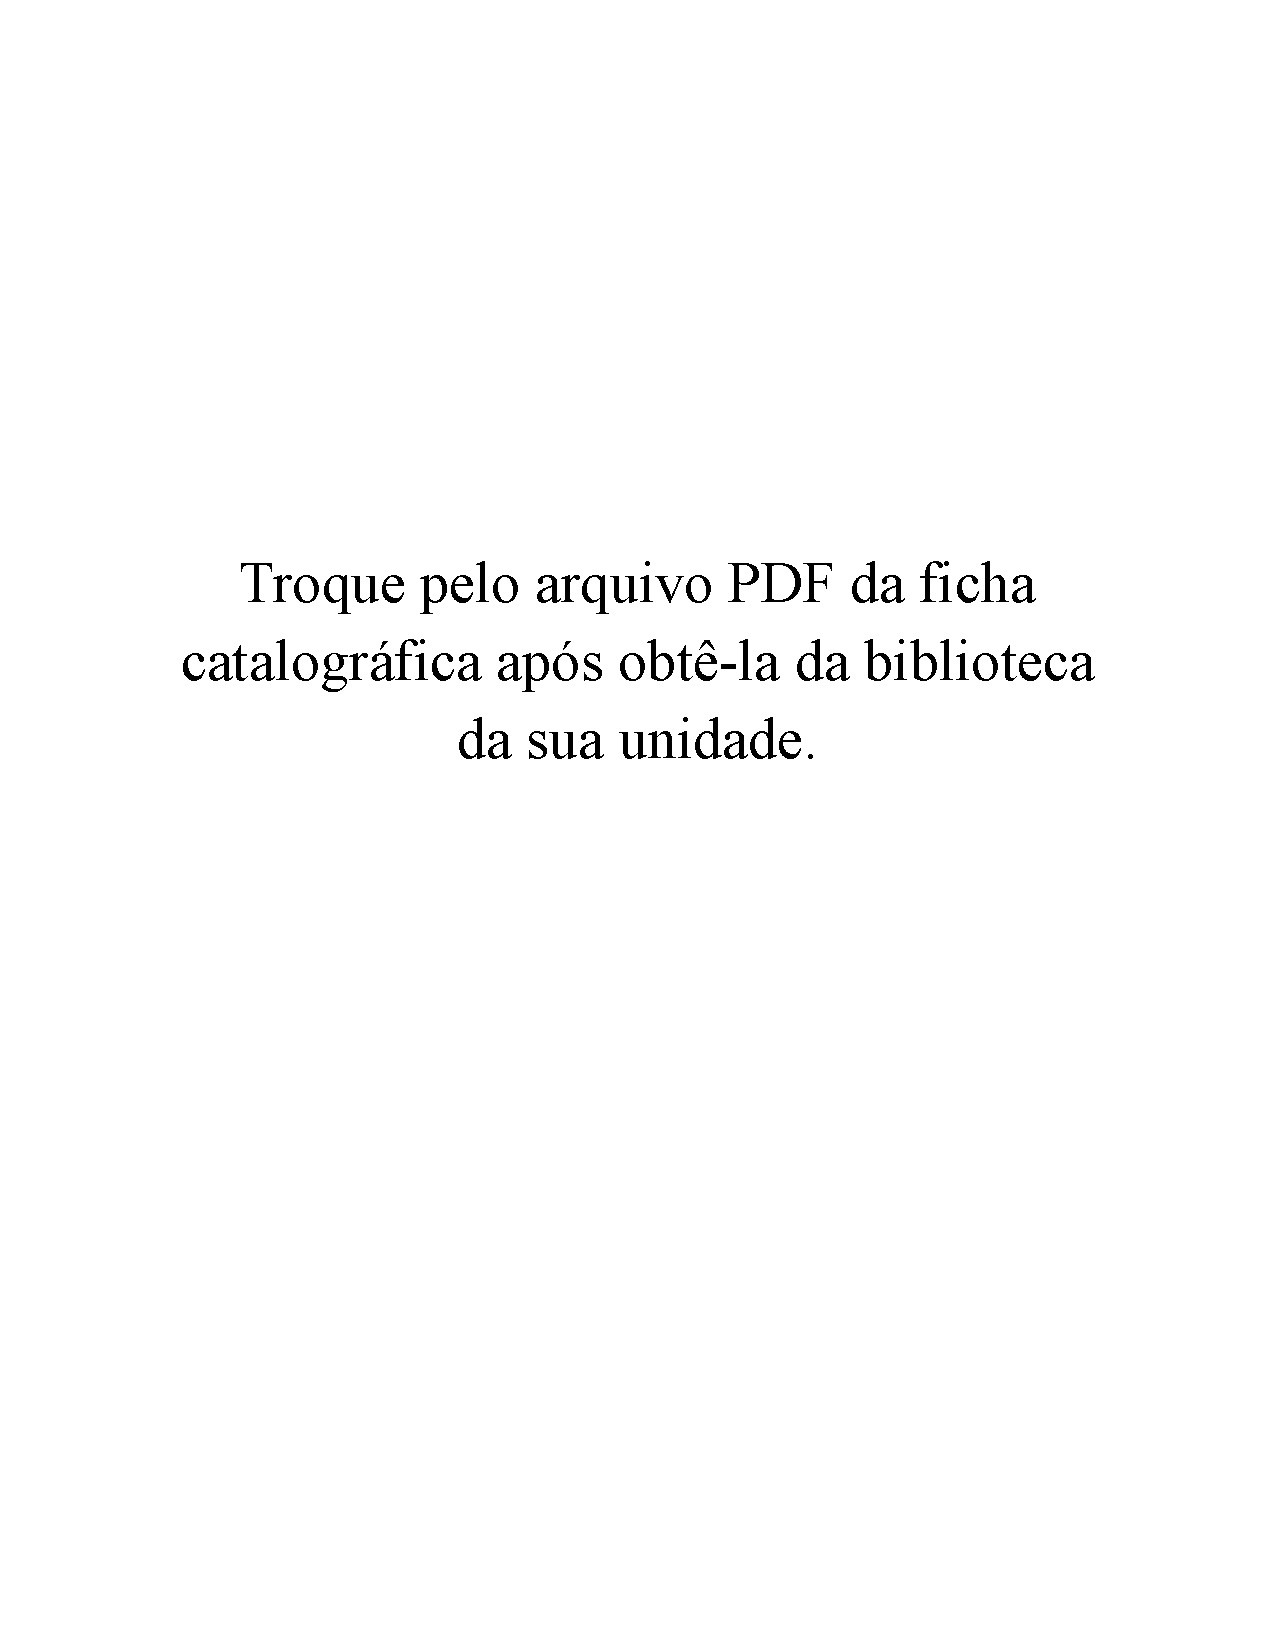
\includepdf{./pretextuais/fichacatalografica}

    % Folha de Aprovação/Ata de defesa: só para trabalhos de mestrado e 
    % doutorado. Caso a ata tenha 2 páginas, você alterar o parâmetro pages={1}
    % para pages={1-2}.	
    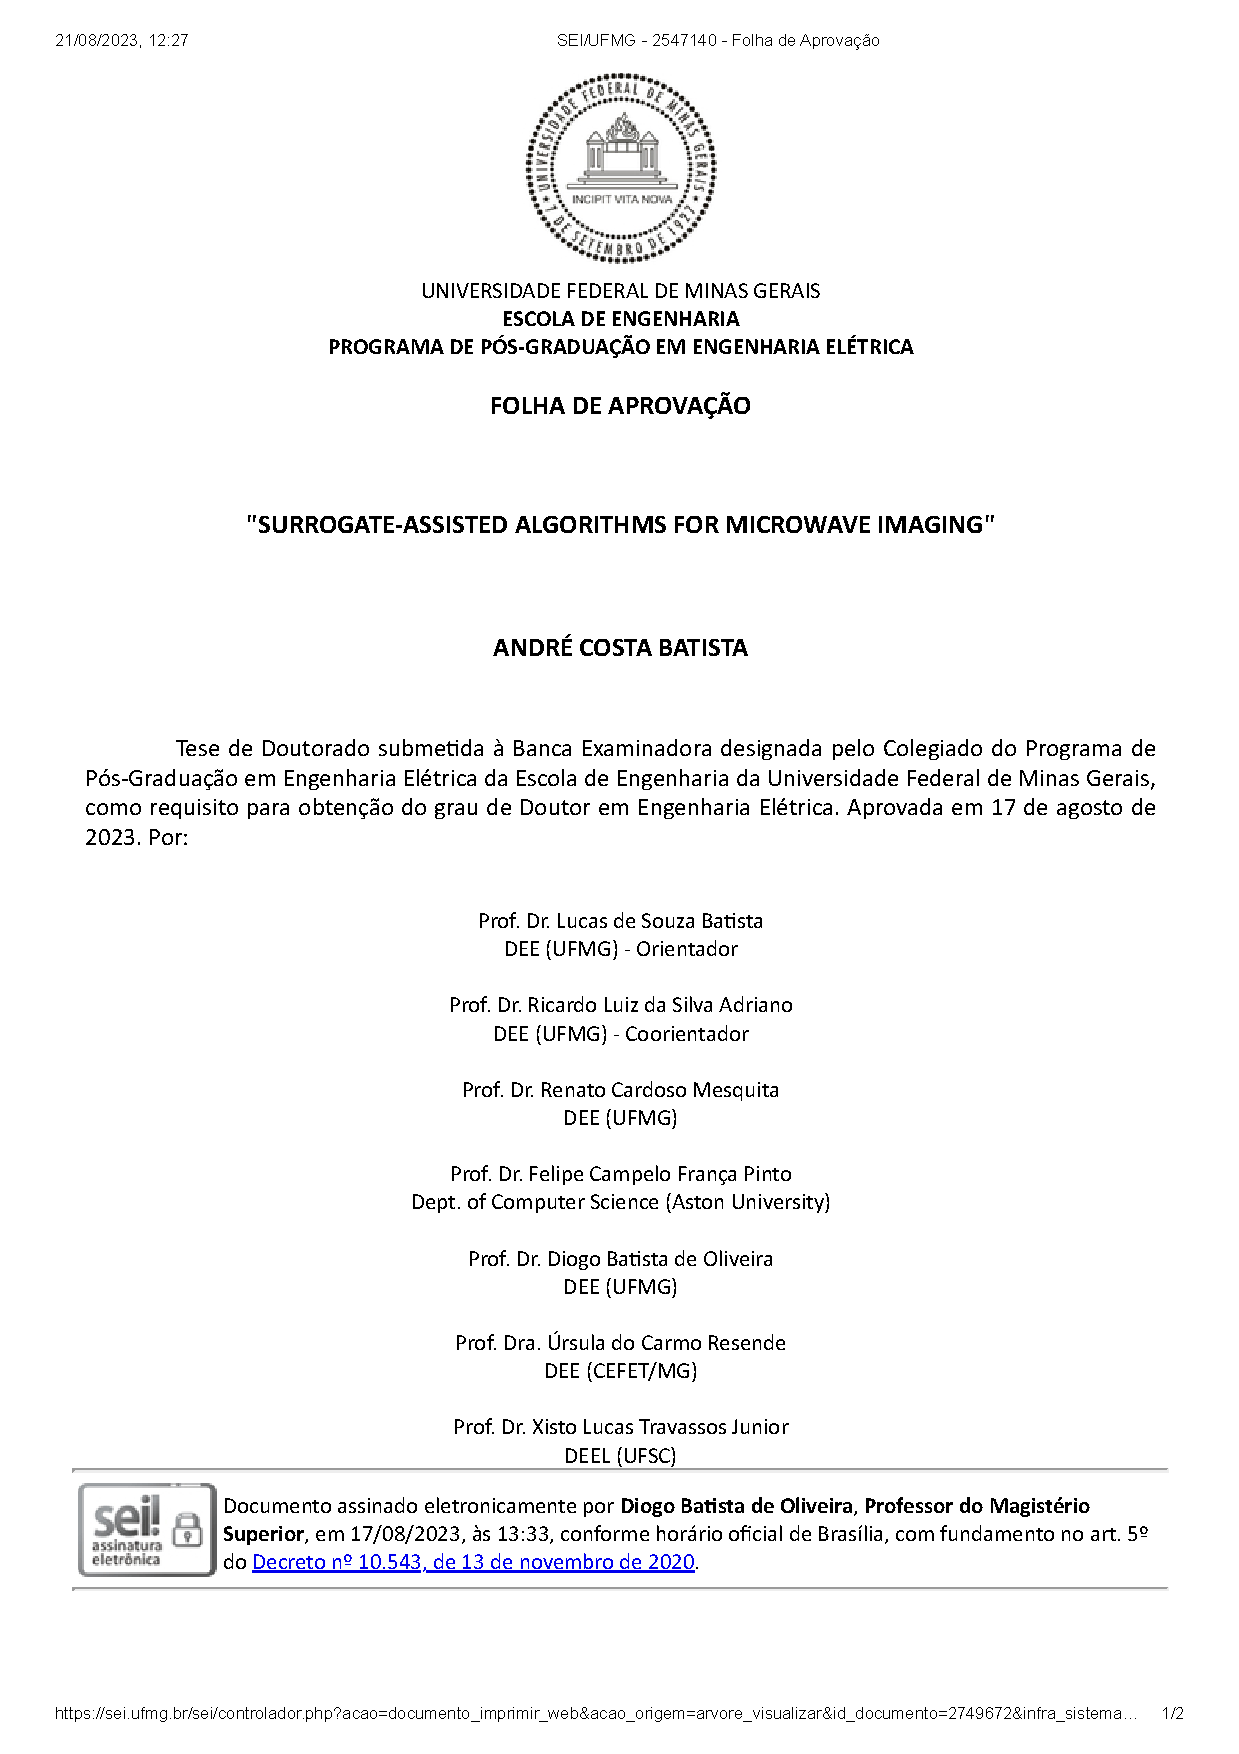
\includepdf[pages={1}]{./pretextuais/folhaaprovacao}

    % Dedicatória
    % A dedicatória, elemento opcional, é utilizada pelo autor para homenagear
% pessoa(s) a quem se dedica o trabalho. O texto é breve, apresentado ao final 
% da página com recuo de 8 cm à esquerda e a página não apresenta título.

\newpage
\thispagestyle{empty}
\vspace*{\fill}
\begin{flushright}
	\hspace{8cm}\textit{Esse trabalho é dedicado à aquela pessoa.}
\end{flushright}

    % Agradecimentos
	% s agradecimentos são destinados à menção de pessoas e instituições que 
% tenham contribuído para o desenvolvimento do trabalho.

\newpage

\chapter*{Agradecimentos} % Inglês: Acknowledgements

	Você pode escrever aqui os agradecimentos a pessoas que contribuíram para a realização do trabalho.
	
	\thispagestyle{empty}

    % Epígrafe
    % As epígrafes são empregadas quando o autor deseja apresentar uma citação 
% direta que estabelece relação com o trabalho apresentado. A página em que 
% consta, não apresenta título “Epígrafe”. Este recurso pode ser utilizado, 
% também, na abertura de cada uma das seções primárias do texto. 

\newpage
\thispagestyle{empty}
\vspace*{\fill}
\begin{flushright}
	``Aqui vai uma bela e inspiradora frase.''
\end{flushright}

    % Resumo e Abstract
	\chapter*{Resumo}

	\noindent O Imageamento em Microondas é uma importante técnica de teste e avaliação não-destrutiva e não-invasiva com muitas aplicações em diversas áreas, como em exames médicos, triagem de segurança, sensoriamento remoto, entre outras. A técnica é baseada em um Problema Inverso de Espalhamento Eletromagnético onde as propriedades elétricas de um meio são recuperadas através de medições de campo espalhado. Além de ser um problema mal-posto, também é não-linear e multimodal. Existem vários métodos numéricos para resolver o problema e eles podem ser classificados em qualitativos ou quantitativos. Estes últimos também são classificados em métodos determinísticos ou estocásticos. Esta tese apresenta uma nova abordagem quantitativa determinística para imageamento em microondas usando algoritmos assistidos por modelos substitutos. O objetivo é abordar os desafios do problema inverso considerando a imagem qualitativa recuperada pelo Método de Amostragem de Ortogonalidade e transformando a imagem em um problema de otimização bidimensional. O método proposto se concentra em otimizar a estimativa de contraste e a operação de limiarização para minimizar o erro da equação de dados. A tese apresenta três formulações baseadas em Algoritmos Evolutivos e duas baseadas em Métodos de Direções de Busca, fornecendo um leque de opções para a resolução do problema de otimização. Além disso, uma nova estrutura é proposta para o desenvolvimento e teste de algoritmos para o problema. A estrutura inclui um pacote abrangente chamado \textit{eispy2d}, que oferece funcionalidades como geração de conjuntos de teste com controle de parâmetros, uma coleção de indicadores de desempenho (incluindo dois novos indicadores) e suporte para comparação estatística de diferentes algoritmos. Os resultados dos experimentos demonstram a eficácia dos métodos propostos. Em cenários com espalhadores fracos, os métodos propostos foram capazes de reconstruir imagens comparáveis àquelas obtidas por métodos tradicionais, enquanto alcançavam tempos de execução próximos. Além disso, em cenários mais desafiadores onde os métodos tradicionais falharam, os algoritmos propostos mostraram resultados consistentes em termos de recuperação de imagens.

	\vspace{5mm}
	
	\noindent\textbf{Palavras-chaves}: imageamento em microondas; problemas inversos; algoritmos assistidos por modelos substitutos; algoritmos evolutivos; métodos de direção de busca; biblioteca de código aberto.
	
	\thispagestyle{empty}
    \chapter*{Abstract}

	\noindent Microwave Imaging is an important nondestructive and noninvasive testing and evaluating technique with many applications in diverse areas, such as medical imaging, security screening, remote sensing, among others. The technique is based on an Electromagnetic Inverse Scattering Problem where the electric properties of a medium are recovered through scattered field measurements. Besides being an ill-posed problem, it is also nonlinear and multimodal. There are several numerical methods for solving the problem and they can be classified into qualitative and quantitative ones. The latter is also classified into deterministic and stochastic methods. This thesis presents a novel quantitative deterministic approach for microwave imaging using surrogate model-assisted algorithms. The objective is to address the challenges of the inverse problem by considering the qualitative image recovered by the Orthogonality Sampling Method and transforming it into a two-dimensional optimization problem. The proposed method focuses on optimizing the contrast estimation and the threshold operation to minimize the data equation error. The thesis introduces three formulations based on Evolutionary Algorithms and two ones based on Descent Methods, providing a range of options for solving the optimization problem. In addition, a new framework is proposed for the development and testing of algorithms in microwave imaging. The framework includes a comprehensive package called \textit{eispy2d}, which offers functionalities such as test set generation with parameter control, a collection of performance indicators (including two novel indicators), and support for statistical comparison of different algorithms. The results of the experiments demonstrate the effectiveness of the proposed methods. In weak scatterer scenarios, the surrogate model-assisted algorithms were able to recover images that were comparable to those obtained by traditional methods, while achieving similar runtimes. Moreover, in more challenging scenarios where traditional methods failed, the proposed algorithms showed consistent results in terms of image recovery.
	
	\vspace{5mm}
	
	\noindent\textbf{Keywords}: microwave imaging; inverse problems; surrogate model-assisted algorithms; evolutionary algorithm; descent methods; open-source package.
	
	\thispagestyle{empty}
	

	% Listas
    \begingroup
    \pagestyle{empty}
    \listoffigures
    \pagestyle{empty}
    \listoftables
    \pagestyle{empty}
    \listofalgorithms
\endgroup
	
    % Abreviações e símbolos
	% Siglas e abreviaturas utilizadas no texto devem ser apresentadas em uma lista 
% alfabética seguida de sua grafia por extenso. A primeira vez que a sigla 
% aparece no texto deve-se pontuar a expressão por extenso, seguida da sigla 
% entre parênteses; nas demais vezes, utiliza-se somente a sigla, inserida
% diretamente no texto.

\newpage
\chapter*{Lista de Siglas e Símbolos} % Inglês: List of Abbreviations and Symbols

	\section*{Siglas}
	
		\begin{itemize}[labelwidth=5em,leftmargin=\dimexpr\labelwidth+\labelsep\relax,align=left]
			\item[ACO] Ant Colony Optimization
			\item[BIM] Born Iterative Method
			\item[CNN] Convolutional Neural Networks
			\item[DE] Differential Evolution
			\item[EA] Evolutionary Algorithm
			\item[GA] Genetic Algorithm
			\item[GAN] Generative Adversarial Network
			\item[PSO] Particle Swarm Optimization
			\item[TMz] Modo Magnético Transversal em $z$
		\end{itemize}
	
		\thispagestyle{empty}

	\section*{Símbolos}
	
		\thispagestyle{empty}
	
		\begin{itemize}[labelwidth=4em,leftmargin=\dimexpr\labelwidth+\labelsep\relax,align=left]
			\item[$\epsilon$] Permissividade complexa [F/m + $j\Omega$/m]
			\item[$\epsilon_r$] Permissividade relativa
			\item[$\theta$] Ângulo da coordenada polar [rad]
			\item[$\lambda_b $] Comprimento de onda de fundo [m]
			\item[$\sigma$] Condutividade [$\Omega$/m]
			\item[$\phi$] Ângulo de incidência [rad]
			\item[$\mathbf{E}$] Vetor de intensidade elétrica [V/m]
			\item[$E_z$] Componente $z$ do vetor de intensidade elétrica [V/m]
			\item[$k$] Número de onda [1/m]
			\item[$\mathbb{R}$] Conjunto dos números reais
			\item[$\mathbf{r}$] Vetor posição no espaço 3D [m]
			\item[$x, y, z$] Coordenadas cartesianas [m]
			\item[$V$] Espaço tridimensional
		\end{itemize}
	
		\thispagestyle{empty}
	
	
    
    % Sumário
    \thispagestyle{empty}
    \tableofcontents

    % Ativa numeração de páginas
    % ATENÇÃO: depois que você terminar de escrever o trabalho, você DEVE
    % voltar aqui acertar o número
    \pagenumbering{arabic}
    \setcounter{page}{12}

    % Introdução
    % ------------------------------------------------------------------------------
% Introdução
% ------------------------------------------------------------------------------

\chapter{Introdução}\label{chap:introducao} % Inglês: Introduction

	Parte inicial do texto na qual se apresenta a delimitação do assunto tratado, os 
	objetivos da pesquisa e outros elementos necessários para apresentar o tema 
	do trabalho. O texto tem o objetivo de introduzir o leitor ao trabalho e 
	apresentar as informações para uma compreensão geral da proposta
	desenvolvida.

	\section{Objetivos Geral e Específicos}\label{sec:introducao:objetivos}

		Descrever os objetivos geral e específicos do trabalho. O objetivo
		geral devem ser claro e conciso, indicando o propósito do trabalho.
		Os objetivos específicos devem ser apresentados de forma a indicar
		os passos necessários para atingir o objetivo geral. Geralmente, em formato de tópicos.

	\section{Contribuições e Originalidade}\label{sec:introducao:contribuicoes}

		Descrever as contribuições do trabalho, indicando o que o trabalho
		propõe de novo ou diferente em relação ao estado da arte. As contribuições
		devem ser claras e objetivas, indicando o que o trabalho agrega ao conhecimento
		existente.
	
	\section{Organização do Trabalho}\label{sec:introducao:organizacao}

		Descrever a organização do trabalho, indicando o conteúdo de cada capítulo
		e a relação entre eles. A organização do trabalho deve ser clara e
		coerente, de forma a facilitar a compreensão do leitor.


    % Revisão Bibliográfica
    % ------------------------------------------------------------------------------
% Revisão Bibliográfica
% ------------------------------------------------------------------------------

\chapter{Revisão Bibliográfica}\label{chap:revisao}

	Ao redigir uma revisão bibliográfica em trabalhos acadêmicos, é crucial adotar uma abordagem sistemática e crítica. Inicie identificando e selecionando fontes relevantes que abordem diretamente o tema de pesquisa, priorizando publicações acadêmicas revisadas por pares, como artigos de periódicos, livros e conferências. Uma boa prática é organizar a literatura em temas ou escolas de pensamento, facilitando a compreensão do leitor sobre o estado da arte e as lacunas existentes. É importante também avaliar criticamente cada obra, discutindo sua contribuição para o campo, metodologias, resultados e limitações. A revisão deve ser escrita de forma coesa, com transições suaves entre os trabalhos discutidos, e deve terminar destacando como a pesquisa atual se insere e contribui para o conhecimento existente. Citando adequadamente todas as fontes, evita-se o plágio e reconhece-se o trabalho dos pesquisadores originais, além de fornecer ao leitor caminhos para aprofundamento.

    % Metodologia
    % ------------------------------------------------------------------------------
% Metodologia
% ------------------------------------------------------------------------------

\chapter{Metodologia}\label{chap:metodologia}

	Redigir um capítulo sobre metodologia em um trabalho acadêmico é fundamental para demonstrar a validade e a confiabilidade da pesquisa. Este capítulo deve detalhar os procedimentos e técnicas utilizados para coletar e analisar dados, permitindo que outros pesquisadores reproduzam o estudo. Aqui estão os passos essenciais para escrever um capítulo de metodologia eficaz:

	\begin{itemize}
		\item Introdução à Metodologia: Comece com uma breve introdução que esclareça o propósito do capítulo e como ele contribui para os objetivos gerais da pesquisa.
		\item Descrição da Pesquisa: Especifique o tipo de pesquisa realizada (qualitativa, quantitativa, mista) e justifique a escolha. Explique como essa abordagem é adequada para responder às perguntas de pesquisa ou hipóteses.
		\item Participantes ou Dados: Descreva a população-alvo, critérios de inclusão e exclusão, e como os participantes ou dados foram selecionados. Para pesquisas experimentais, explique como os grupos de controle e experimentais foram formados.
		\item Instrumentos e Materiais: Liste os instrumentos, ferramentas, ou materiais utilizados na coleta de dados, incluindo questionários, entrevistas, software, etc. Descreva como e por que cada instrumento foi escolhido.
		\item Procedimento: Detalhe todos os passos seguidos durante a coleta de dados. Para experimentos, descreva as condições sob as quais foram realizados, incluindo variáveis controladas e não controladas.
		\item Análise de Dados: Explique as técnicas estatísticas, métodos de análise qualitativa, ou modelos utilizados para analisar os dados coletados. Justifique a escolha desses métodos e discuta sua adequação para o tipo de dados coletados.
		\item Validade e Confiabilidade: Discuta as medidas tomadas para garantir a validade e confiabilidade dos resultados. Isso pode incluir a validação de instrumentos, triangulação de dados, ou testes piloto.
		\item Limitações: Reconheça quaisquer limitações metodológicas que possam afetar os resultados ou a interpretação da pesquisa.
		\item Ética: Se aplicável, descreva as considerações éticas relacionadas à pesquisa, incluindo aprovações de comitês de ética, consentimento informado dos participantes, e como a privacidade e a confidencialidade foram mantidas.
		\item Resumo: Conclua o capítulo com um resumo dos pontos-chave, reforçando como a metodologia adotada permite abordar as perguntas de pesquisa ou testar as hipóteses.
	\end{itemize}

	Lembre-se de que a clareza e a precisão são cruciais neste capítulo. O objetivo é fornecer informações suficientes para que outros pesquisadores possam entender como o estudo foi conduzido e, se desejado, replicar a pesquisa.
    
    % ------------------------------------------------------------------------------
% Proposed Methodology
% ------------------------------------------------------------------------------

\chapter{Proposed Methodology}\label{chap:proposed-methodology}

	This thesis aims to enhance the current state-of-the-art algorithms for microwave imaging by proposing novel approaches based on surrogate models. Additionally, a comprehensive framework for the development and testing of algorithms specific to this problem is presented. In Section \ref{chap:proposed-methodology:criticism}, a critical review of the literature is presented, highlighting the gaps and areas for improvement in the current state of the art. Building on this analysis, Section \ref{chap:proposed-methodology:proposal} proposes a novel approach to address some of the limitations, specifically, the use of surrogate models and the framework for development and comparison of algorithms designed for EISPs. Section \ref{chap:proposed-methodology:surrogate} provides a detailed discussion of surrogate-model assisted algorithms for microwave imaging, including a description of the transformation of the inversion problem into a bidimensional optimization one, the Kriging model, and the proposed algorithms. Section \ref{chap:proposed-methodology:library} outlines a framework for developing and testing algorithms for microwave imaging, including the proposed metrics to assess their performance. Finally, Section \ref{chap:proposed-methodology:conclusion} presents the concluding remarks.

	\section{Literature Criticism and Opportunities}\label{chap:proposed-methodology:criticism}
	
		In the early stages of developing algorithms for microwave imaging, several challenges were encountered \citep{kirsch2011introduction,pastorino2000microwave,bertero2020introduction}. In the early context, the available data was significantly limited and noisy, which represented a serious challenge for a problem with non-unique solution. When more data was available, the limited computing power was other challenge. The understanding of the physics involved in microwave imaging also evolved throughout the years, which was also important for the development of the subject.
	
		Currently, two significant challenges are faced by researchers in the literature: real-time imaging and the retrievement of strong scatterers. Real-time imaging requires fast and efficient algorithms that can produce accurate images in real-time or nearly, which is essential for many applications such as medical imaging \citep{li2021machine} and security screening \citep{asok2022concealed}. To address this challenge, researchers have turned to deep-learning techniques that can efficiently process large amounts of data and provide accurate results in real-time \citep{salucci2022artificial}.
		
		The other challenge is the imaging of strong scatterers, which refers to objects with high contrast levels or large dimensions when comparing to the wavelength. Such objects result in high nonlinearity and can create significant artifacts in the resulting image, making it difficult to accurately reconstruct the underlying structure. This is particularly challenging when imaging complex structures, such as biological tissues or composite materials \citep{lazebnik2007large}. This type of scenario has been addressed in three main ways:
		\begin{enumerate}
			\item The first approach is to reduce the degree of non-linearity by changing the integrals solved by the algorithms (Section \ref{chap:problemstatement:eisp});
			\item The second approach is based on domain decomposition \citep{zhang2022iterative}. This approach divides the scatterer region into dominant and subordinate subdomains based on the information of the induced current. The dominant subdomain is then reconstructed iteratively, narrowing the inversion domain and reducing the nonlinearity of the problem.
			\item The third approach is the use of surrogate models \citep{koziel2008engineering}. \cite{salucci2022learned} proposed a surrogate model to predict the data equation error considering curve-based representations of scatterers. By using this approach, the computational cost of stochastic algorithms that do not solve the contrast and the total field simultaneously can be significantly reduced. This is because such algorithms rely on forward problem simulations to estimate the error. The authors demonstrated the effectiveness of their approach in high-contrast scenarios, showing promising results.
		\end{enumerate}
		
		Some ideas in the field have yet to receive the attention they deserve, and one of them is the use of qualitative methods to define initial solutions for quantitative algorithms. Even though this approach has been explored in some papers \citep{zhang2020learning,han2022hybrid,bevacqua2015algebraic}, it has yet to be fully utilized to improve the performance of stochastic algorithms for the problem. The use of qualitative methods can help to improve the robustness of images reconstructed by these algorithms to noise and high contrasts, as well as guide the convergence of population-based algorithms towards more promising regions of the search space.
		
		%Outro aspecto que chama a atenção na literatura é o design dos experimentos e a avaliação da qualidade dos algoritmos. É necessário destacar que um aspecto extremamente relevante para a experimentação é a utilização de modelos de espalhadores mais realísticos ou dados obtidos de medições reais. Isto tem ficado popular na literatura através laboratórios que disponibilização os dados. Dois exemplos muito comuns são o \textit{UWCEM Numerical Breast Phantom Repository} \citep{burfeindt2012mri} e as medições realizadas pelo \textit{Institut Fresnel} \citep{geffrin2005free}. 
		Another aspect that draws attention in the literature is experiment design and quality evaluation of algorithms. A highly relevant aspect of experimentation is using more realistic scatterer models or data obtained from real measurements. This has become popular in the literature through laboratories that make the data available. Two widespread examples are the \textit{UWCEM Numerical Breast Phantom Repository} \citep{burfeindt2012mri}  and the measurements made by the \textit{Institut Fresnel} \citep{geffrin2005free}.
		
		In addition, \cite{kurrant2021evaluating} have recently proposed a methodology to evaluate the performance of the algorithms applied to breast cancer detection. Given a reference image and the recovered one, the authors proposed to segment the tissues in the images by an unsupervised machine learning approach. After decomposing the images and mapping the tissues, five metrics were proposed to evaluate shape fidelity, malignant tissue reconstruction in tumor regions, among others. Therefore, the novelty is a technique to measure the quality of breast reconstruction with suitable tools. Their methodology is also available as a MATLAB toolbox \citep{kurrant2021mwsegeval}.
		
		%No entanto, os autores das publicações tradicionalmente escolhem instâncias com características particulares com o objetivo de demonstrar a capacidade de reconstrução do método proposto na correspondente situação. A partir disso, a performance é medida através de algum indicador de qualidade e o resultado é comparado a outros algoritmos e formulações \citep{zhong2020multiresolution,zhang2020wavelet,zhou2021improved}. Embora essa abordagem seja interessante para ilustrar a capacidade do algoritmo, ela tem pouco rigor metodológico para oferecer respostas robustas à perguntas como: (i) qual impacto da escolha da instância no valor do quantificador da performance? (ii) Como o indicador varia se a geometria do objeto mudar? (iii) Como a diferença na performance observada entre os dois métodos varia se as geometrias variarem? (iv) Qual a performance média ou pior caso do método para uma dada configuração? (v) Etc.
		However, in many publications addressing general applications, traditional instances have been chosen with particular characteristics to demonstrate the reconstruction ability of the proposed method in the corresponding situation. Performance is measured through some quality indicator, and the result is compared to other algorithms and formulations \citep{zhong2020multiresolution,zhang2020wavelet,zhou2021improved}. Although this approach is interesting to illustrate the algorithm's suitableness, it has little methodological rigor to offer robust answers to questions such as: (i) what is the impact of the choice of the instance on the performance quantifier's value? (ii) How does the indicator vary if the object's geometry changes? (iii) How does the difference in performance observed between the two methods vary if the geometries vary? (iv) What is the average or worst-case performance of the method for a given configuration? Among others.
		
		%Mesmo que essas perguntas possam fugir do escopo de propostas baseadas em um estudos de caso (e.g., experimentos reais), conclusões gerais sobre a capacidade e performance podem ser muito fracas sem uma metodologia experimental adequada que leve em consideração diferentes fatores de efeito na configuração do problema. Embora o fator de nível de ruído costume ser o mais explorado nesse sentido \citep{chew1990reconstruction,chen2010subspace,shah2018fast,batista2021quadratic}, uma experimentação com instâncias aleatórias para uma medição mais robusta da performance não foi levada em consideração nem quando a publicação tinha como objetivo principal a comparação entre algoritmos \citep{moghaddam1991comparison,gilmore2009comparison,pan2010comparison}. Este tipo de prática é essencial para eliminar o viés do observador em análises de algoritmos \citep{montgomery2010applied}. Um outro exemplo sobre isso é a existência de vários trabalhos na literatura que propõem metodologias estocásticas e nem ao menos informam quantas vezes o algoritmo foi repetido quando exibem o resultado para uma dada instância. Não há informação se o resultado mostrado representa o pior, médio ou melhor caso, como se fosse o resultado único de um tipo de metodologia que não tem garantia nenhuma de retornar a mesma solução em toda execução \citep{massa2005parallel,ashtari2010using,salucci2017multifrequency}.
		Even though these questions may fall outside the scope of proposals based on case studies (e.g., physical experiments), general conclusions about suitability and performance can be very weak without an adequate experimental methodology that considers different effect factors in the configuration of the problem. Although the noise level factor is usually the most explored in this sense \citep{chew1990reconstruction,chen2010subspace,shah2018fast,batista2021quadratic}, experiments with random instances for a more robust measurement performance are not usually performed. Even when the publication had the main objective of comparing algorithms \citep{moghaddam1991comparison,gilmore2009comparison,pan2010comparison}. This practice is essential to eliminate the observer's bias in algorithms analysis \citep{montgomery2010applied}. Other examples are several works in the literature that propose stochastic methodologies and do not even inform how many times the algorithm was repeated when showing the result for a given instance. There is no information if the result shown represents the worst, average, or best case. This is problematic since these methodologies have no guarantee of returning the same solution in every execution \citep{massa2005parallel,ashtari2010using,salucci2017multifrequency}.
		
		%Por isso, uma oportunidade na literatura é introduzir comparações mais robustas entre algoritmos. Uma referência sobre boas práticas de comparação de algoritmos de otimização é o artigo escrito por \cite{beiranvand2017best}. Entre muitos apontamentos relevantes feitos pelos os autores, destacamos os seguintes:
		Therefore, another opportunity in the literature is to introduce more robust comparisons between algorithms, i.e., benchmarking. A reference on best practices for comparing optimization algorithms is the article written by \cite{beiranvand2017best}. Among the many relevant notes made by the authors, we highlight the following:
		
		\begin{itemize}
			%\item Um conjunto de teste com poucos problemas deve ser referido como um estudo de caso ou prova de conceito, mas não benchmarking.
			%\item Um conjunto de teste deve evitar as seguintes deficiências: (i) poucos problemas; (ii) pouca ou excessiva variação na complexidade das instâncias inviabilizando a extração de informações úteis; (iii) problemas sem soluções conhecidas (o qual pode ser inevitável em situações reais); (iv) viés no ponto de partida dos algoritmos; (v) estruturas escondidas (e.g., arredondamento de números). 
			%\item Todos algoritmos devem receber a mesma quantidade de informação de entrada e garantir que não há um pressuposto que é respeitado somente por um dos algoritmos.
			\item A test suite with few problems should be referred to as a case study or proof of concept, but not benchmarking.
			\item A test suite should avoid the following deficiencies: (i) few problems; (ii) slight or excessive variation in the complexity of the instances, making it impossible to extract helpful information; (iii) problems with no known solutions (which can be inevitable in real situations); (iv) bias at the starting point of the algorithms; (v) hidden structures.
			\item All algorithms must receive the same amount of input information and ensure that there is an assumption that is only respected by one of the algorithms in order to verify the influence of that assumption.
		\end{itemize}
		
		%Esses tópicos não representam necessariamente falhas nas experimentações descritas na literatura. No entanto, esses conceitos já estabelecidos na literatura sobre otimização podem trazer amadurecimento na de algoritmos para EISP.
		These topics do not necessarily represent failures in the experiments described in the literature. However, these concepts already established in the optimization literature can bring maturity to the algorithms for EISP.
		
		%Por fim, destacamos também as métricas utilizadas para avaliar a qualidade das reconstruções. Na vasta maioria dos trabalhos, a qualidade das imagens reconstruídas da função contraste é quantificada por uma das seguintes formas \citep{wang1989iterative,chew1990reconstruction,shah20193d,oliveri2019compressive,oliveri2011multiresolution,salucci2017multifrequency,zhang2020learning}:
		Finally, we also highlight the metrics used to assess the quality of the reconstructions. In the vast majority of works, the quality of the reconstructed images of the contrast function is quantified in one of the following ways \citep{wang1989iterative,chew1990reconstruction,shah20193d,oliveri2019compressive,oliveri2011multiresolution,salucci2017multifrequency,zhang2020learning}:
		\begin{align}
			\zeta_{\epsilon} &= \sqrt{\frac{1}{N_IN_J}\sum\limits_{i=1}^{I}\sum\limits_{j=1}^J\left|\frac{\epsilon^*_{r,ij}-\epsilon_{r,ij}}{\epsilon^*_{r,ij}}\right|^2} \label{eq:4:error0:epsilon} \\
			\zeta_{\chi} &= \sqrt{\frac{1}{N_IN_J}\sum\limits_{i=1}^{I}\sum\limits_{j=1}^J\left|\frac{\chi^*_{ij}-\chi_{ij}}{\chi^*_{ij}+1}\right|^2} \label{eq:4:error0:chi}
		\end{align}
		
		%\noindent onde $\epsilon^*_{r,ij}$ e $\chi^*_{ij}$ são os valores verdadeiros de permissividade relativa e contraste, respectivamente. Ou seja, de um modo geral, \eqref{eq:4:error0:epsilon} e \eqref{eq:4:error0:chi} são fórmulas baseadas na raiz da média do erro percentual. Pequenas variações nelas também podem ser adotadas, como a substituição de $N_IN_J$ pela área da imagem ou pela remoção da raiz e do quadrado do erro.
		\noindent where $\epsilon^*_{r,ij}$ and $\chi^*_{ij}$ are the actual values of relative permittivity and contrast, respectively. In general, \eqref{eq:4:error0:epsilon} and \eqref{eq:4:error0:chi} are formulas based on the root of the average percentage error. Slight variations can also be adopted, such as replacing $N_IN_J$ with the image area or removing the root and square of the error.
		
		%De um modo geral, quando se trata de identificar objetos na imagem, uma boa reconstrução é caracterizada pela identificação correta da posição, da forma e do contraste do espalhador. \eqref{eq:4:error0:epsilon} e \eqref{eq:4:error0:chi} são métricas que abordam essas três características ao mesmo. Uma reconstrução igual à verdadeira vai minimizar esses indicadores. No entanto, existem situações nas quais esses indicadores não são tão eficientes. Quando a área de um espalhador é muito menor que a da figura, o erro vai ser bem pequeno mesmo que haja muitos desvios na estimativa do contraste na área do espalhador (e.g., $\chi=0$). Isto pode também disfarçar erros significativos na posição e forma dos espalhadores reconstruídos. Vale à pena notar que os resíduos das equações não são tomados necessariamente como medidores de qualidade tendo em vista que, por causa da má-posição do problema, podem haver soluções com baixo resíduos e imagens diferentes das esperadas.
		In general, when it comes to identifying objects in the image, a good reconstruction is characterized by the correct identification of the scatterer's position, shape, and contrast. \eqref{eq:4:error0:epsilon} and \eqref{eq:4:error0:chi} are metrics that address these three characteristics at the same time. A reconstruction equal to the actual one will minimize these indicators. However, there are situations in which these indicators are not as efficient. When the area of a scatterer is much smaller than the figure, the error will be minimal. This might happen even if there are many deviations in the estimate of the contrast in the scatterer area (e.g., $\chi=0$). This can also disguise significant errors in the position and shape of the rebuilt scatterers. It is worth noting that the residuals of the equations are not necessarily taken as quality meters, given that, due to ill-posedness, there may be solutions with low residues and images that are different from those expected.
		
		%Conforme sugerido por \cite{beiranvand2017best}, outros indicadores também podem avaliar aspectos interessantes do desempenho dos algoritmos: (i) taxa de sucesso, i.e., quantidade de vezes que um algoritmo atinge uma determinada tolerância em um determinado tempo-limite; (ii) percentual de soluções encontradas em uma dada situação; (iii) perfil de precisão, i.e., porcentagem de problemas que um algoritmo consegue resolver para um dado percentual de precisão; (iii) perfil de performance, i.e., probabilidade que um algoritmo resolva um problema dado um limite de tempo; entre outros. Estes indicadores poderiam fornecer informações enriqueceriam muito a comparação dos algoritmos.
		As suggested by \cite{beiranvand2017best}, other indicators can also evaluate interesting aspects of algorithms performance: (i) success rate, i.e., the number of times that an algorithm reaches a certain tolerance in a specific time limit; (ii) percentage of a class of solutions found in a given situation; (iii) accuracy profile, i.e., percentage of problems that an algorithm can solve for a given percentage of accuracy; (iii) performance profile, i.e., the probability that an algorithm will solve a problem given a time limit; among others. These indicators could provide information that would greatly enrich the comparison of the algorithms.
	
	\section{Proposal}\label{chap:proposed-methodology:proposal}
	
		%Levando em consideração a discussão na seção anterior sobre o estado-da-arte e das oportunidades das lacunas presentes na literatura, esta pesquisa tem duas propostas de contribuição: (i) o projeto de algoritmos assistidos por modelos substitutos que se baseiam nas imagens geradas por métodos qualitivativos e (ii) o projeto de um software especializado para o desenvolvimento e testagem de algoritmos para o problema, com suporte a testagem randomizada e medição de performance média através de um conjunto de indicadores. Portanto, o objetivo é explorar uma nova possibilidade de aplicação de modelos substitutos que aproveite das vantagens do uso de métodos qualitativos para obtenção de soluções iniciais para o problema quantitativo. Ao mesmo tempo, o trabalho visa trazer mais robustez às análises de algoritmos para o problema.
		
		In the previous section, the state-of-the-art and the gaps in the literature on the inverse electromagnetic scattering problem were discussed. Based on this discussion, two contributions are proposed by our research. First, algorithms assisted by surrogate models that use images generated by qualitative methods are aimed to be designed. Second, the design of specialized software for the development and testing of algorithms for this problem is proposed, with support for randomized testing and measurement of average performance through a set of indicators. These contributions aim to explore new possibilities of applying surrogate models and bring more robustness to the analysis of algorithms for the problem.
		
		%A busca por novas aplicações de modelos substitutos no problema é encorajada tendo em vista que a introdução desta técnica é recente e explorada apenas por \cite{salucci2022learned}. Se por um lado a representação de espalhadores por curvas que definem seus contornos permitem uma reconstrução compatível com geometrias complexas, por outro lado ela exige um número de váriaveis que, embora seja muito menor do que representações baseadas em pixels, ainda pode ser muito alta para os modelos substitutos. Além disso, é necessário saber de antemão quantos espalhadores existem na imagem para que sejam definidos o número de contornos compatível. Se a imagem obtida pelos métodos qualitativos for aproveitada, o problema se torna em estimar o contraste o contraste dos objetos e ajustar o limiar que separa o meio de fundo dos objetos. Em outras palavras, isto tornaria a inversão em um problema de otimização bidimensional, no qual a performance de modelos substitutos é mais elevada. Além disso, tendo em vista que o OSM é capaz de captar diferentes níveis de contraste nas imagens, a aplicação em casos de múltiplos objetos de diferentes níveis de contraste seria viável. No entanto, a aplicação fica restrita aos casos onde os métodos qualitativos funcionam adequadamente, i.e., objetos cujo o contraste e as dimensões não fossem capazes de ser reconstruídos pelos métodos qualitativos tampouco seriam obtidos pelo processo de otimização assistido pelo modelo substituto. De uma maneira geral, esta abordagem pode ser vista como a transformação de uma metodologia qualitativa em uma quantitativa a partir de sua redefinição como um problema de otimização bidimensional e redução do custo computacional através da assistência de modelos substitutos.
		
		New applications of surrogate models in this problem are encouraged since their introduction is recent and has only been explored by \cite{salucci2022learned}. Using curves to represent scatterers that define their contours allows a reconstruction compatible with complex geometries, but it requires several variables, which can still be very high for surrogate models \citep{wu2019developed}. Furthermore, it is necessary to know beforehand how many scatterers exist in the image so that the compatible number of contours can be defined. If the image obtained by qualitative methods is used, the problem becomes one of estimating the contrast of the objects and adjusting the threshold that separates the background from the objects. In other words, this would turn the inversion process into a two-dimensional optimization problem, in which the performance of surrogate models is higher. The OSM can capture different levels of contrast in the images, making the application feasible in cases of multiple objects with different levels of contrast. However, the application is restricted to cases where the qualitative methods work properly.
		
		%Já a proposição de uma estrutura para algoritmos para o problema de espalhamento eletromagnético inverso é encorajada pela facilitação da implementação e testagem dos mesmos.
		
		As a second contribution, a framework for algorithms for the inverse electromagnetic scattering problem is proposed to facilitate their implementation and testing. Suitable experiments need to be designed to assess the impact of modifications on the performance of algorithms. Arbitrary situations can illustrate the ability of methods to make good reconstructions, and experiments with real data are relevant to attest to the application in practical situations. However, measuring the performance of methods and making comparisons need to follow principles such as control of effect factors and random instances, which are well-established in the specialized literature on Evolutionary Algorithms but little widespread in the literature on methods for Electromagnetic Inverse Scattering. A framework that addresses the insulation of effects factors and new indicators can better qualify the algorithm’s reconstruction performance. This applies not only to stochastic methods but also to deterministic ones.
	
	\section{Surrogate model-Assisted Algorithms for EISPs}\label{chap:proposed-methodology:surrogate}

		This section focuses on the proposed application of surrogate models to solve the electromagnetic inverse scattering problem. To address it, a bi-dimensional optimization approach is employed, where the objective function represents the discrepancy between the estimation of the scattered field and the measured data. Surrogate models have proven to be effective tools in approximating complex objective functions in optimization problems. Therefore, the section also introduces the concept of surrogate models and their application in solving electromagnetic inverse scattering problems. The Kriging model, a popular surrogate modeling technique, is briefly explained, followed by a description of the proposed algorithms that employ the Kriging model to solve the inverse scattering problem.

		\subsection{The Optimization Model}\label{chap:proposed-methodology:surrogate:optimization}
		
			%Os métodos qualitativos de inversão são baseados em cálculos que atribuem um valor a um ponto da imagem através de uma função indicadora. Dependendo do nível desse valor, o ponto é classificado como pertencente a um espalhador ou não. Logo, uma forma simples de transformar o problema qualitativo em um quantitativo seria, dada a imagem obtida pela função indicadora normalizada, determinar o melhor limiar de classificação e a estimativa do contraste na região do objeto. No entanto, o método OSM, além de classificar, é capaz de indentificar diferentes níveis de contraste na imagem, o que possibilita a aplicação em cenário com múltiplos espalhadores de diferentes contrastes.
			
			Qualitative inversion methods are commonly employed when only the shape of objects needs to be retrieved. The method operates by classifying image points as either part of a scatterer or not, based on an indicator function that assigns a value to each point. However, these methods do not offer a quantitative estimate of the scatterer's contrast, meaning they do not estimate the dielectric properties of the objects. One possible solution is to transform the qualitative problem into a quantitative one by identifying the best classification threshold and estimating the contrast in the object region, based on the image obtained from the normalized indicator function. Furthermore, the Orthogonality Sampling Method (OSM), discussed in subsection \ref{chap:methods:qualitative:osm}, not only classifies the points but also identifies different levels of contrast in the image. This ability makes it possible to apply a qualitative method in scenarios with multiple scatterers of different contrasts, which is particularly useful in the field of electromagnetic scattering.
			
			Mathematically, let $\boldsymbol{\chi}^{norm}$ be the $N_I\times N_J$ image obtained by OSM in which the pixel values are normalized between 0 and 1. Then, a quantitative inversion result could be obtained if (i) a threshold level $T$ is applied to separate background and scatterers, i.e., set $\chi^{norm}_{ij} = 0$ for pixels where $\chi^{norm}_{ij} < T$; and (ii) multiply the remaining non-zero pixels by a factor $\chi^F$. In other words, a new quantitative image $\boldsymbol{\chi}$ is obtained by:
			\begin{equation}
				\chi_{ij} = \begin{cases}
					\chi^F\chi^{norm}_{ij},& \text{if }\chi^{norm}_{ij} \ge T, \\
					0, & \text{otherwise.}
				\end{cases} \label{eq:proposed-methodology:surrogate:optimization:transformation}
			\end{equation}
			
			% Each step of the proposed process is illustrated in Figure \ref{fig:proposed-methodology:surrogate:optimization:transformation}. The transformation does not prevent contrast variations within the contrast area, since homogeneity is not assumed \textit{a priori}. If homogeneity is assumed, then the truncation by the average value might be performed.
			Figure \ref{fig:proposed-methodology:surrogate:optimization:transformation} illustrates each step of the proposed process. Note that the transformation does not assume homogeneity within the contrast area, which means that contrast variations are allowed. However, if homogeneity is assumed, the truncation by the average value can be performed.
			
			\begin{figure}[!h]
				\centering
				\subfloat[]{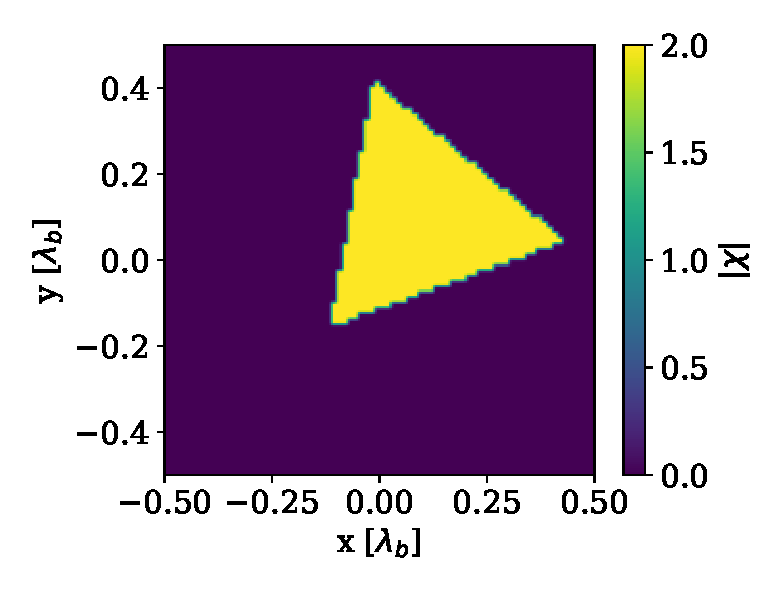
\includegraphics[width=.4\textwidth]{./figuras/transformation_original}} \hspace{.05\textwidth}
				\subfloat[]{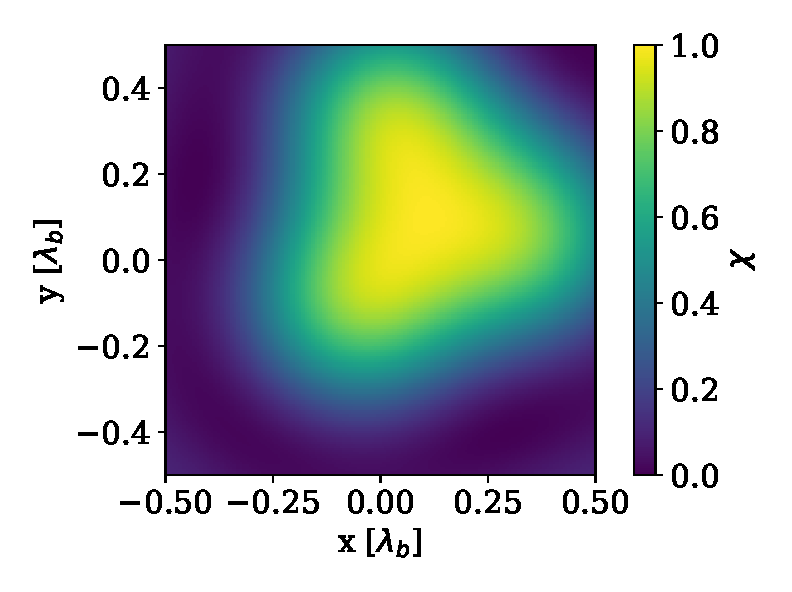
\includegraphics[width=.4\textwidth]{./figuras/transformation_thresholding}} \\
				\subfloat[]{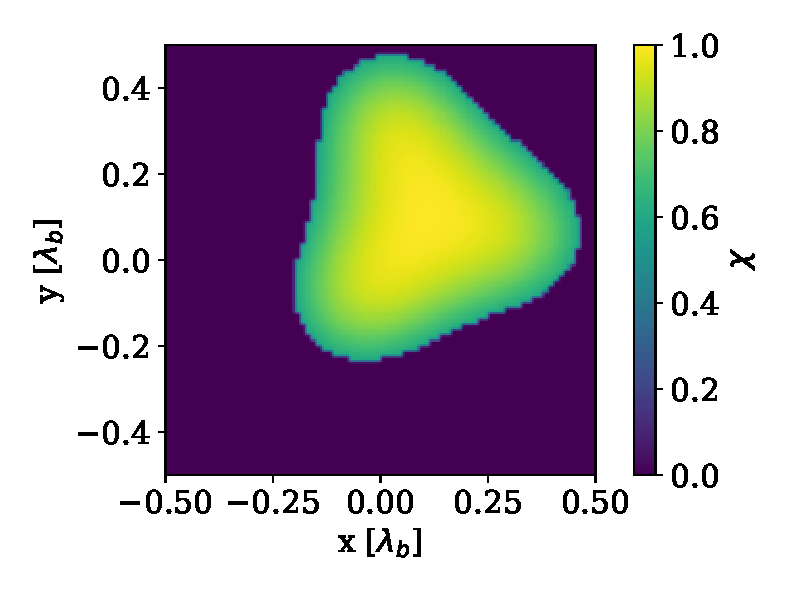
\includegraphics[width=.4\textwidth]{./figuras/transformation_multiplication}} \hspace{.05\textwidth}
				\subfloat[]{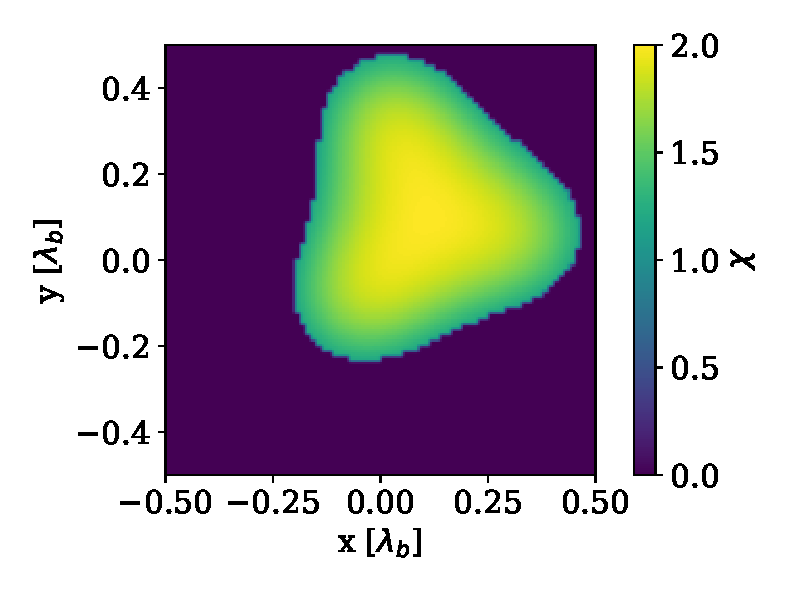
\includegraphics[width=.4\textwidth]{./figuras/transformation_final}}
				\caption[Example of the process of transforming a qualitative image into a quantitative one.]{Example of the process of transforming a qualitative image into a quantitative one: (a) ground-truth image; (b) image obtained by OSM ($\boldsymbol{\chi}^{norm}$); (c) image obtained after the thresholding process; and (d) final image obtained after the multiplication step.}
				\label{fig:proposed-methodology:surrogate:optimization:transformation}
			\end{figure}
			
			%The image $\boldsymbol{\chi}$ is also the diagonal elements of the contrast matrix $\boldsymbol{\bar{\chi}}$ in \eqref{eq:3:discretization:collocation:18}. Thus, the data equation error \eqref{eq:3:discretization:collocation:10} might be computed if the total electric field was also evaluated. Therefore, for a given scattered field data and the corresponding Green function matrix, the following bidimensional optimization problem might be defined:'
			The image $\boldsymbol{\chi}$ represents the diagonal elements of the contrast matrix $\boldsymbol{\bar{\chi}}$ mentioned in \eqref{eq:3:discretization:collocation:18}. Consequently, the data equation error \eqref{eq:3:discretization:collocation:10} can be calculated only if the total electric field is evaluated. Hence, a two-dimensional optimization problem can be defined based on a given scattered field data and its corresponding Green function matrix.
			\begin{align}
				T^*, \chi^{F*} =&~\arg\min f(T, \chi^F) \label{eq:proposed-methodology:surrogate:optimization:definition:objfun} \\
				& T\in[0, 1],~ \chi^{F} \in [\chi^F_{min}, \chi^F_{max}] \label{eq:proposed-methodology:surrogate:optimization:definition:bounds} 
			\end{align}
			
			\noindent where $ f(T, \chi^F)$ is the function that determines the data equation error based on the process of solving qualitatively the inverse problem through OSM and applying the transformation according \eqref{eq:proposed-methodology:surrogate:optimization:transformation}. Evidently, the total field must be computed for each pair $(T, \chi^F)$.
			
			%1. Um aspecto importante para qualquer problema de otimização são as características da função objetivo.			
			%2. No problema abordado, enquanto a variação da fator de multiplicação produz variações contínuas no erro da equação de dados, a variação do limiar não produz em pequena escala.
			%3. Uma vez que a imagem é uma representação discreta da função contraste, variações muito pequenas no operador de limiarização podem não causar mudança nenhuma na imagem resultante. Ou seja, se eu variar a variável T de modo que ela não alcance o menor valor de X dentro do objeto, a imagem não muda. Logo, o valor da função objetivo é constante nesse pequeno intervalo.
			Understanding the characteristics of the objective function is crucial for solving any optimization problem effectively. This is because the choice of the most appropriate algorithm depends on this information. Therefore, having knowledge of the objective function's properties is essential for selecting the best optimization method and achieving the desired outcome.
			
			In the optimization problem defined by \eqref{eq:proposed-methodology:surrogate:optimization:definition:objfun}-\eqref{eq:proposed-methodology:surrogate:optimization:definition:bounds}, varying the multiplication factor $\chi^F$ leads to continuous variations in the error of the data equation. However, varying the threshold $T$ does not produce a significant change on a small scale. This is due to the fact that the image is a discrete representation of the contrast function, and small variations in the thresholding operator may not cause any change in the resulting image. Hence, the value of the objective function remains constant in this small interval.
			
			%4. Este efeito ocorre em pequena escala. Ou seja, numa perspectiva macro da função objetivo, ela vai parecer suave e possivelmente até convexa. No entanto, quando se visualizarmos a superfície da função numa escala bem reduzida, notaremos discontinuidades na função. O que permite dizer que a função é multi-escala.
			%5. Isto pode trazer problemas para aplicação de métodos de otimização que se baseiam na informação da derivada. Isto porque a estimativa da derivada se dá pela avaliação da função num local vizinho da solução atual a qual está distante por um valor discreto de uma das variáveis. Logo, o ajuste desse valor discreto para perturbação da solução pode se tornar complicado pois, se o método estiver perto de uma discontinuidade, então o gradiente pode apontar para uma direção errada. Nesses casos, métodos sem-derivadas ou métodos baseados em população podem ser mais eficientes.
			Although this effect occurs on a small scale and the objective function appears smooth and convex from a macro perspective, when we visualize the surface of the function on a smaller scale, we will notice non-smoothness. This makes the function multi-scale and can create problems for optimization methods that depend on derivative information. When close to a roughness, the adjustment of the discrete value for perturbation of the solution might be complicated, making the gradient point in the wrong direction. Derivative-free methods or population-based methods may be more efficient in such cases.
			
			\begin{figure}[!h]
				\centering
				\subfloat[]{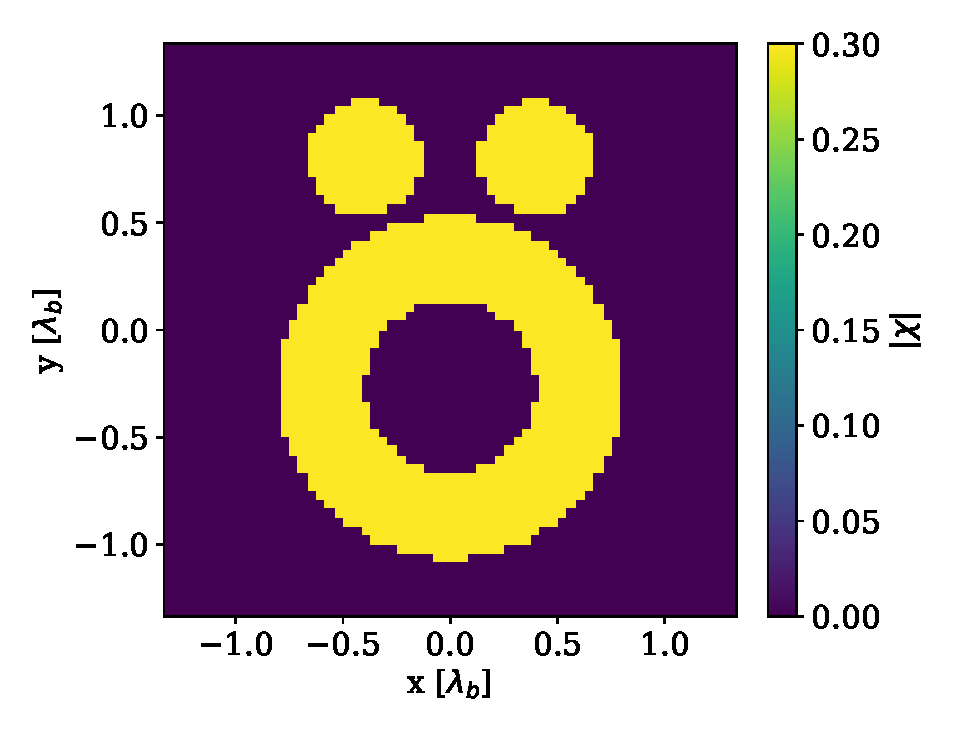
\includegraphics[width=.4\textwidth]{./figuras/objfun_groundtruth}\label{fig:proposed-methodology:surrogate:optimization:objfun:groundtruth}} \hspace{.05\textwidth}
				\subfloat[]{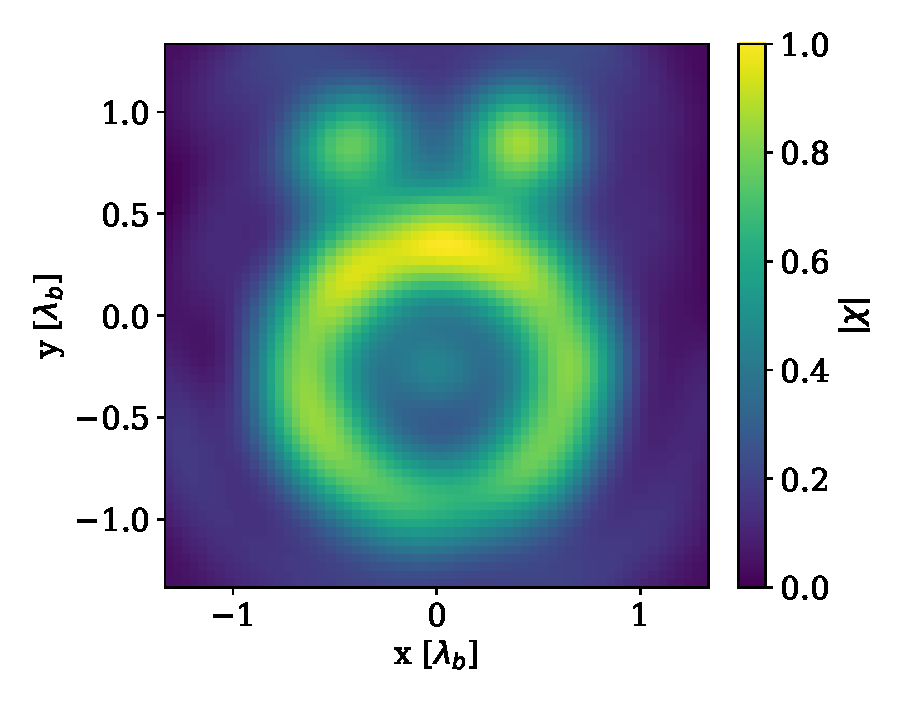
\includegraphics[width=.4\textwidth]{./figuras/objfun_qualitative}\label{fig:proposed-methodology:surrogate:optimization:objfun:qualitative}} \\
				\subfloat[]{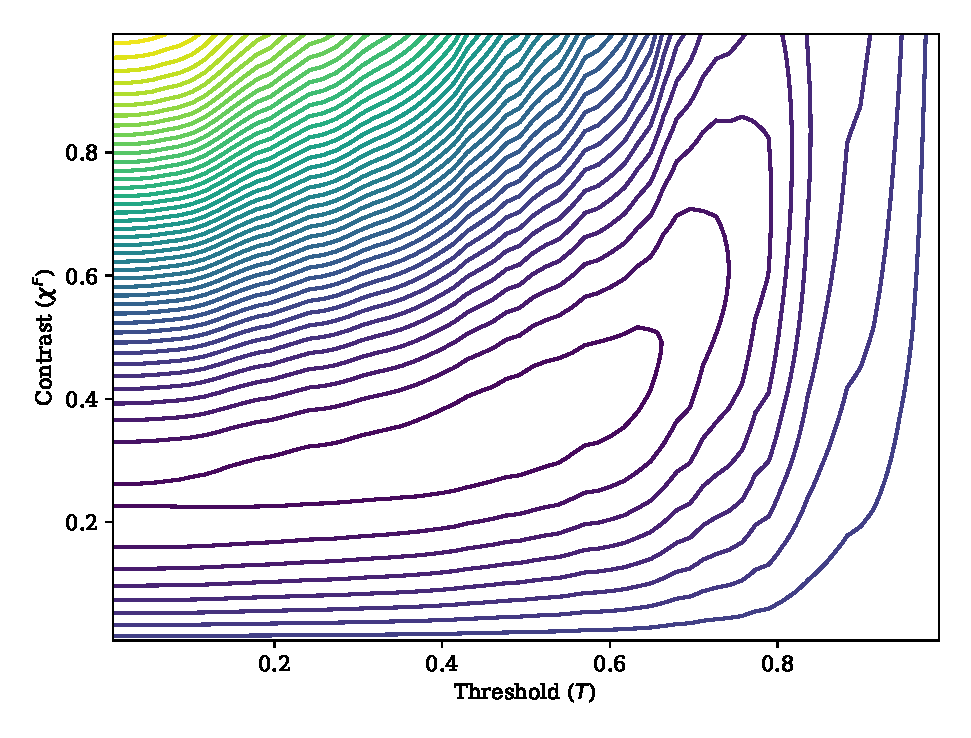
\includegraphics[width=.4\textwidth]{./figuras/objfun_surface}\label{fig:proposed-methodology:surrogate:optimization:objfun:surface}} \hspace{.05\textwidth}
				\subfloat[]{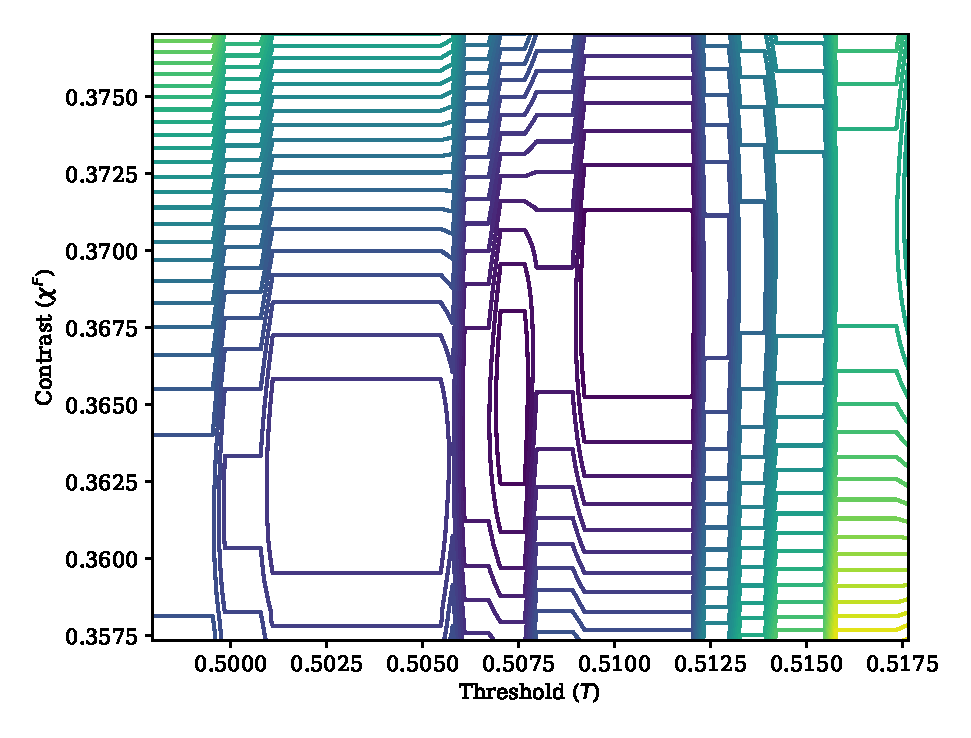
\includegraphics[width=.4\textwidth]{./figuras/objfun_nearoptimum}\label{fig:proposed-methodology:surrogate:optimization:objfun:nearoptimum}}
				\caption[Example of an objective function resulting from the transformation of the inversion problem into a two-dimensional optimization one.]{Example of an objective function resulting from the transformation of the inversion problem into a two-dimensional optimization one: (a) the ground-truth image; (b) the image obtained by OSM; (c) the surface obtained by the transformation of the inversion problem into a two-dimensional optimization one; and (d) a zoom over the region close to the optimum.}
				\label{fig:proposed-methodology:surrogate:optimization:objfun}
			\end{figure}
			
			%6. A figura 4 ilustra este problema. A figura 4(b) mostra a reconstrução a partir do método qualitativo para um teste representado pela figura 4(a). Na figura 4(c) vemos a superfície da função objetivo resultante da transformação do problema de inversão em um problema de otimização bidimensional. Como é possível notar, a superfície, numa perspectiva macro, parece bem suave. No entanto, quando ampliamos a imagem para perto do ótimo (figura 4(d)), vemos as discontinuidades no eixo da variável T.
			Figure \ref{fig:proposed-methodology:surrogate:optimization:objfun} illustrates this problem. Figure \ref{fig:proposed-methodology:surrogate:optimization:objfun:qualitative} shows the reconstruction from the qualitative method for a test represented by Figure \ref{fig:proposed-methodology:surrogate:optimization:objfun:groundtruth}. In Figure \ref{fig:proposed-methodology:surrogate:optimization:objfun:surface}, we see the surface of the objective function resulting from the transformation of the inversion problem into a two-dimensional optimization problem. The surface appears smooth from a macro perspective, but when we zoom in on the image close to the optimum (Figure \ref{fig:proposed-methodology:surrogate:optimization:objfun:nearoptimum}), we see the roughness on the $T$ variable axis.
			
			%7. Outra questão é que o valor ótimo do fator de multiplicação pode não coincidir com o valor exato do contraste da imagem, principalmente em casos de espalhadores homogêneos. Isto porque as variações de contraste dentro da região do objeto impossibilitam reconstruir com exatidão a imagem. Isto é possível obser pela figura 4(d). Uma alternativa para mitigar este efeito é assumir que o objeto é todo homogêneo e truncar os valores dentro da região do objeto pelo seu valor médio ou máximo.
			Another issue is that the optimal value of the multiplication factor may not coincide with the exact value of the image contrast, mainly in cases of homogeneous scatterers. This is because contrast variations within the object region make it difficult to accurately reconstruct the image. An alternative to mitigate this effect is to assume that the object is all homogeneous and truncate the values within the object's region by their average or maximum value.
			
			%8. Por fim, vale à pena frisar que a avaliação da função objetivo não é barata, uma vez que esta depende da execução do resolvedor direto para estimar o campo total correspondente. Logo, pode ser proibitivo a aplicação de um algoritmo de otimização que dependa de muitas avaliações.
			Finally, it is worth emphasizing that the evaluation of the objective function is not cheap since it depends on the execution of the direct resolver to estimate the corresponding total field. Therefore, applying an optimization algorithm that depends on many evaluations can be prohibitive.

		\subsection{Surrogate Models}\label{chap:proposed-methodology:surrogate:explanation}
			
			In many optimization problems, the objective function can be computationally expensive to evaluate, meaning that it takes a long time to compute the value of the function for a given set of input parameters. This can make it difficult to find good quality solutions, as it may take many iterations of the optimization algorithm to explore the search space thoroughly.
			
			Surrogate Models are approximations of the expensive objective function that are designed to reduce the computational cost of evaluating the objective function \citep{schonlau1997computer,mendes2013surrogate,sacks1989design}. A surrogate model is typically trained on a set of input-output pairs, where the inputs are the parameters of the optimization problem and the outputs are the value of the objective function for those parameters. The surrogate model learns to approximate the objective function using this training data, allowing it to make predictions about the value of the objective function for new sets of input parameters without actually evaluating the expensive objective function.
			
			Surrogate models can be used to speed up the convergence of optimization algorithms, as the surrogate model can be evaluated much more quickly than the expensive objective function. This means that the optimization algorithm can explore the search space more quickly, potentially finding good quality solutions in fewer iterations. Additionally, the use of surrogate models can reduce the number of evaluations of the expensive objective function, which can be a significant computational cost in some problems \citep{sobester2008engineering}.
			
			There are many different types of surrogate models, including regression models, neural networks, and Gaussian processes, among others. In this thesis, the Kriging model is considered since it is widely used in optimization problems \citep{emmerich2006single,zhao2011metamodeling,yang2019two} and it has shown slightly better performance in single-objective optimization problems \citep{valadao2020comparative}. 
			
			% The choice of surrogate model will depend on the specific problem and the available data. In some cases, it may be necessary to use multiple surrogate models or to combine surrogate models with other optimization techniques in order to achieve the best results.
		
		\subsection{Kriging Model}\label{chap:proposed-methodology:surrogate:kriging}
		
			Let $y : \mathbb{X} \subset \mathbb{R}^n \Rightarrow \mathbb{R}$ be an objective function for a given problem. A sample with $N$ solutions and their respective evaluations are $\mathbf{X} =  [\mathbf{x}^1, \cdots, \mathbf{x}^N]^T$ and $\mathbf{y} = [y(\mathbf{x}^1), \cdots, y(\mathbf{x}^N)]^T$, respectively. The Kriging model is a regression model where each observation of the objective function is treated as \citep{sacks1989design,schonlau1997computer,jones1998efficient}:
			\begin{equation}
				y(\mathbf{x}^i) = f(\mathbf{x}^i) + e(\mathbf{x}^i),~ i = 1, \cdots, N \label{eq:kriging:responsemodel}
			\end{equation}
		
			\noindent where $f(\mathbf{x}^i) = \mathbf{f}^T\boldsymbol{\alpha} = \sum\limits_{k=0}^d \alpha_kf_k(\mathbf{x}^i)$, $d\le N-1$, is a linear combination of the regression functions $f_k(\cdot)$ and $\alpha_k$, $k=0,\cdots,d$, are the corresponding coefficients; $e(\cdot)$ is a random normal variable with zero mean and variance $\Sigma^2$. Regression functions are similar to the trial functions presented in Section \ref{chap:methods:discretization}. In the scope of present subsection:
			\begin{equation}
				f_k(\mathbf{x}) = \prod\limits_{r=1}^n x_r^{q_r},~ q_r \in [0, Q],~ \sum\limits_{r=1}^n q_r \le Q \label{eq:kriging:trialfunctions}
			\end{equation}

			\noindent where $Q$ is the highest integer that satisfies $\frac{(n+Q)!}{Q!n!} < N-1$ \citep{zhao2011metamodeling}. The covariance of $e(\cdot)$ is assumed as:
			\begin{equation}
				Cov(e(\mathbf{x}^i), e(\mathbf{x}^j)) = \Sigma^2R(\boldsymbol{\theta},\mathbf{x}^i,\mathbf{x}^j) \label{eq:kriging:covariance}
			\end{equation}
		
			\noindent where $R(\cdot, \cdot, \cdot)$ is a Gaussian correlation function whose form is:
			\begin{equation}
				R(\boldsymbol{\theta},\mathbf{x}^i,\mathbf{x}^j) = \prod\limits_{r=1}^n e^{-\theta_r|x_r^i-x_r^j|^2} \label{eq:kriging:gaussiancorrelation}
			\end{equation}
		
			\noindent with $\boldsymbol{\theta} \in \mathbb{H}$, $\mathbb{H} = \left\{[\theta_1,\cdots,\theta_n]|\theta_r>0\forall r=1,\cdots,n\right\}$. Other correlation functions are also possible \citep{sacks1989design,mackay1998introduction}. However, \eqref{eq:kriging:gaussiancorrelation} is often used when the Kriging model is considered \citep{jin2005comprehensive,zhao2011metamodeling}. The parameters $\boldsymbol{\theta}$ are estimated based on the available sample and they mean the importance of each variable and how correlated they are.
			
			The optimal choice of $\boldsymbol{\theta}$, based on the sample data, is defined as the maximum likelihood estimator (MLE), where the likelihood funnction has the following form:
			\begin{equation}
				L(\boldsymbol{\theta}) = \frac{1}{\sqrt{(2\pi\Sigma^2)^N|\mathbf{R}|}}\mathrm{exp}\left(-\frac{1}{2\Sigma^2}(\mathbf{y}-\mathbf{F}\boldsymbol{\alpha})^T\mathbf{R}^{-1}(\mathbf{y}-\mathbf{F}\boldsymbol{\alpha})\right) \label{eq:kriging:mle}
			\end{equation}
		
			\noindent where $\mathbf{F}=[f_k(\mathbf{x}^i)]_{N\times(d+1)}$ and $\mathbf{R} = [R(\boldsymbol{\theta},\mathbf{x}^i,\mathbf{x}^j)]_{N\times N}$ are the regression and correlation matrices, respectively, with $i,j\in {1,\cdots, N}$ and $k\in {0,\cdots,d}$. For a given $\boldsymbol{\theta}$, the expressions:
			\begin{eqnarray}
				\boldsymbol{\hat{\alpha}} &=& \left(\mathbf{F}^T\mathbf{R}^{-1}\mathbf{F}\right)^{-1}\mathbf{F}^T\mathbf{R}^{-1}\mathbf{y} \label{eq:kriging:alphamle} \\
				\hat{\Sigma}^2 = \frac{1}{N} \left(\mathbf{y}-\mathbf{F}\boldsymbol{\hat{\alpha}}\right)^T\mathbf{R}^{-1}(\mathbf{y}-\mathbf{F}\boldsymbol{\hat{\alpha}}) \label{eq:kriging:sigma2mle}
			\end{eqnarray}
		
			\noindent provide the respective MLEs of $\boldsymbol{\alpha}$ and $\Sigma^2$. If \eqref{eq:kriging:alphamle} and \eqref{eq:kriging:sigma2mle} are used in \eqref{eq:kriging:mle}, then the optimal $\boldsymbol{\theta}$ is obtained through:
			\begin{equation}
				\arg\max\limits_{\boldsymbol{\theta}\in \mathbb{H}} \ln~L(\boldsymbol{\theta}) \label{eq:kriging:optimization}
			\end{equation}
		
			\noindent where:
			\begin{equation}
				\ln~L(\boldsymbol{\theta}) = -\frac{N}{2}\ln(2\pi) - N\ln(\hat{\Sigma}) - \ln(|\mathbf{R}|) - \frac{1}{2}
			\end{equation}
		
			By determining the optimal $\boldsymbol{\theta}$ through \eqref{eq:kriging:optimization}, the correlation matrix $\mathbf{R}$ is obtained and $\boldsymbol{\hat{\alpha}}$ and $\hat{\Sigma}^2$ are computed according to \eqref{eq:kriging:alphamle} and \eqref{eq:kriging:sigma2mle}, respectively. Then, for an untried input $\mathbf{x}$, the predicted evaluation and its mean squared error are, respectively:
			\begin{eqnarray}
				\hat{y}(\mathbf{x}) &=& \mathbf{f}^T\boldsymbol{\hat{\alpha}} + \mathbf{r}^T\mathbf{R}^{-1}(y-\mathbf{F}\boldsymbol{\hat{\alpha}}) \label{eq:kriging:prediction} \\
				\hat{s}^2(\mathbf{x}) &=& \hat{\Sigma}^2\left[1-\left(\mathbf{f}^T(\mathbf{x})+\mathbf{r}^T(\mathbf{x})\right) \begin{pmatrix} \mathbf{0} & \mathbf{F}^T \\ \mathbf{F} & \mathbf{R} \end{pmatrix}^{-1} \begin{pmatrix} \mathbf{f}(\mathbf{x}) \\ \mathbf{r}(\mathbf{x}) \end{pmatrix} \right]
			\end{eqnarray}
		
			\noindent where $\mathbf{r}^T(\mathbf{x}) = \left[R(\boldsymbol{\theta}, \mathbf{x}^1, \mathbf{x}), \cdots, R(\boldsymbol{\theta}, \mathbf{x}^N, \mathbf{x})\right]$ is the vector of correlation; $R(\boldsymbol{\theta}, \mathbf{x}^i, \mathbf{x})$ represents the correlation between $e(\cdot)$ at the sampled point $\mathbf{x}^i$ and $e(\cdot)$ at an untried $\mathbf{x}$, for $i=1,\cdots,N$. 
			
			Finally, such Kriging model is an interpolation model. Interestingly, when \eqref{eq:kriging:prediction} is evaluated at a point that belongs to the sample, then the prediction is the actual evaluation. This is due to the matching of $\mathbf{r}^T$ for the considered point with a line of the matrix $\mathbf{R}$.

		\subsection{Surrogate model-Assisted Algorithms}\label{chap:proposed-methodology:surrogate:algorithms}
		
			% 1. Na subseção 3.1, foi visto que a função-objetivo resultante da transformação do problema inversão em um de otimização bidimensional, além de ser multi-escala, é também cara computacionalmente. Estas características decorrem da não-suavidade do operador de limiarização e da necessidade de solução do problema direto para estimativa do erro.
			% 2. Uma alternativa para esses dois problemas é a substituição da função objetivo por um modelo substituto. Tendo em vista que o modelo substituto é um operador de interpolação, ele pode contornar o problema da micro-escala. Ou seja, reconstruir a função-objetivo pelas suas características macroscópicas através de um conjunto de pontos na superfície que não são muito próximos. O modelo substituto será uma função suave desde que use funções de base suaves. Além disso, a predição da avaliação da função objetivo é um processo muito mais barato do que a avaliação em si. Portanto, fica mais viável a aplicação de algoritmos de direção de busca e de população também.
			
			The chapter presented various aspects related to the proposed optimization problem and the use of surrogate models. Subsection \ref{chap:proposed-methodology:surrogate:optimization} showed how the inversion problem was transformed into a two-dimensional optimization problem. However, the obtained objective function is non-smooth and computationally expensive due to the non-smoothness of the thresholding operator and the need to solve the problem directly to estimate the data equation error. To address these challenges, one alternative is to use a surrogate model, which can reconstruct the objective function by considering its macroscopic characteristics through a set of surface points that are not too close together. The surrogate model works as an interpolation operator and can overcome the microscale problem, resulting in a smooth function when smooth basis functions are used. Additionally, predicting the objective function evaluation is less costly than evaluating it, making it feasible to apply search direction and population-based algorithms.
			
			% 3. De uma maneira geral, um algoritmo assistido por modelos substitutos dependem de, em primeiro lugar, obter uma amostra de pontos no espaço de busca com suas respectivas avaliações. Com essa amostra, o modelo substituto da função objetivo é construído. A partir daí, o processo de busca pode ser iniciado e, simulateamente, o modelo substituto é atualizado a partir de novas soluções encontradas e escolhidas para serem avaliadas pela função objetivo. Portanto, além das diferentes formas de obter o conjunto inicial, é possível explorar diferentes metodologias de busca e de atualização do modelo.
			In order to implement an algorithm assisted by surrogate models, the first step is to obtain a sample of points in the search space along with their respective evaluations. Based on this sample, the surrogate model of the objective function can be constructed. Once the surrogate model is obtained, the search process can begin, and the model can be updated with new solutions that are chosen to be evaluated by the objective function. Thus, in addition to the various methods for obtaining the initial set of points, it is also possible to explore different methodologies for searching and updating the surrogate model.
			
			% 4. Com relação às metodologias de obtenção da amostra inicial de soluções para o modelo substituto, uma forma trivial é a amostragem uniforme do espaço de busca. Ou seja, dados os intervalos das variáveis de decisão, são amostrados pontos equidistantes em cada eixo. No entanto, a abordagem mais tradicional é a Latin Hypercube Sampling (LHS) \cite{iman1981apporach}. It is a statistical method that generates quasi-random sampling distributions. It is widely used in computer experiments due to its simplicity and its projection properties in high-dimensional problems. To construct the LHS design, each variable dimension space is divided into n sections, where n represents the number of sampling points. Then, only one point is placed in each of the sections.
			One way to obtain the initial sample of solutions is through uniform sampling of the search space. This involves sampling equidistant points on each axis within the range of decision variables. However, the more traditional approach is Latin Hypercube Sampling (LHS) \cite{iman1981apporach}, which is a statistical method that generates quasi-random sampling distributions. LHS is widely used in computer experiments due to its simplicity and projection properties in high-dimensional problems. To construct the LHS design, the space of each variable dimension is divided into n sections, where n is the number of sampling points. Only one point is then placed in each section.

			
			% 5. Para ilustrar possíveis diferenças entre esses dois métodos de amostragem, foi simulado um problema de um espalhador de alto contraste (Figura 5a). Note que a função objetivo (Figura 5b)  é multimodal. A amostragem pelo método LHS resulta na superfície da Figura 5c, enquanto a obtida pela amostragem uniforme é apresentada na Figura 5d. Note que, na superfície obtida pelo LHS, existe uma barreira separando a região original do mínimo em duas. Nessa separação, não existe nenhuma amostra. Uma vez que o método LHS é estocástico, então cada amostragem pode resultar numa superfície diferente e regiões importantes podem ficar sem nenhuma amostra. Na amostragem uniforme, também não é garantido que uma região fique sem amostras. Principalmente se o número de amostras for baixo. Mas, com um número razoável de amostras, pode-se chegar a uma superfície com características mais parecidas principalmente quando o problema é bidimensional, como é o caso do exemplo da Figura 5. Portanto, para evitar os aspecto estocástico na amostragem, a metodologia uniforme será adotada sendo necessário escolher sempre um número adequado de amostras.
			To illustrate the differences between these two sampling methods, a high-contrast scatterer problem was simulated (Figure \ref{fig:proposed-methodology:surrogate:algorithms:samplings:groundtruth}), resulting in a multimodal objective function (Figure \ref{fig:proposed-methodology:surrogate:algorithms:samplings:objfun}. Sampling by the LHS method resulted in a surface with a barrier separating the original minimum region in two, in which there was no sample (Figure \ref{fig:proposed-methodology:surrogate:algorithms:samplings:objfun}). Since the LHS method is stochastic, each sampling can result in a different surface, and important regions can be left without any samples. Uniform sampling can also result in regions running out of samples, especially if the number of samples is low. However, with a reasonable number of samples, a surface with similar characteristics can be obtained, especially in two-dimensional problems, as it is shown in Figure \ref{fig:proposed-methodology:surrogate:algorithms:samplings:uniform}. Therefore, to avoid the stochastic aspect of sampling, a uniform methodology is adopted, and it is always necessary to choose an adequate number of samples.

			\begin{figure}[!h]
				\centering
				\subfloat[]{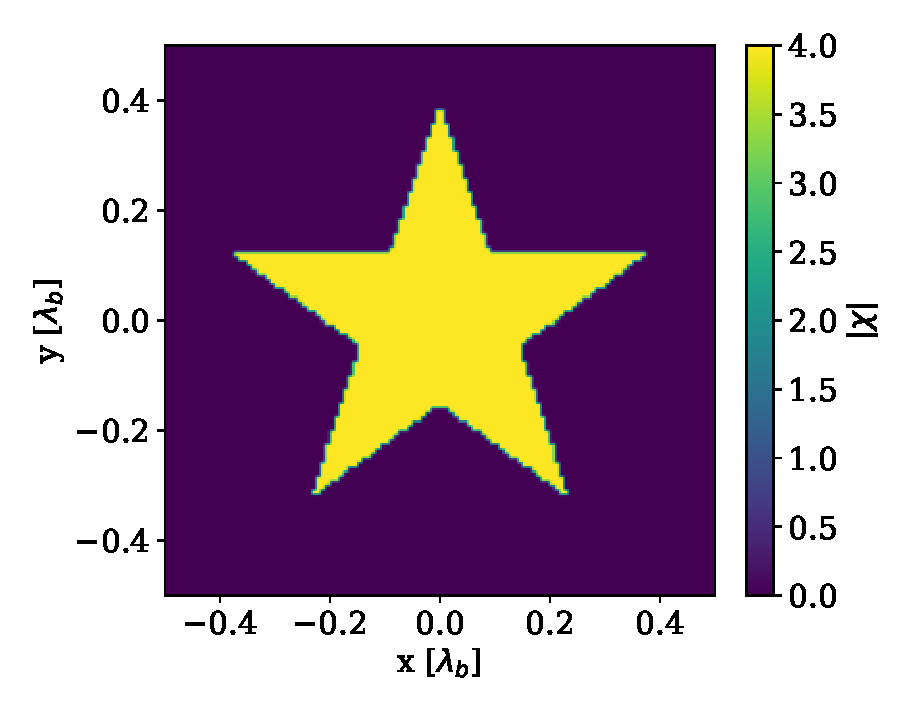
\includegraphics[width=.4\textwidth]{./figuras/samplings_groundtruth}\label{fig:proposed-methodology:surrogate:algorithms:samplings:groundtruth}} \hspace{.1\textwidth}
				\subfloat[]{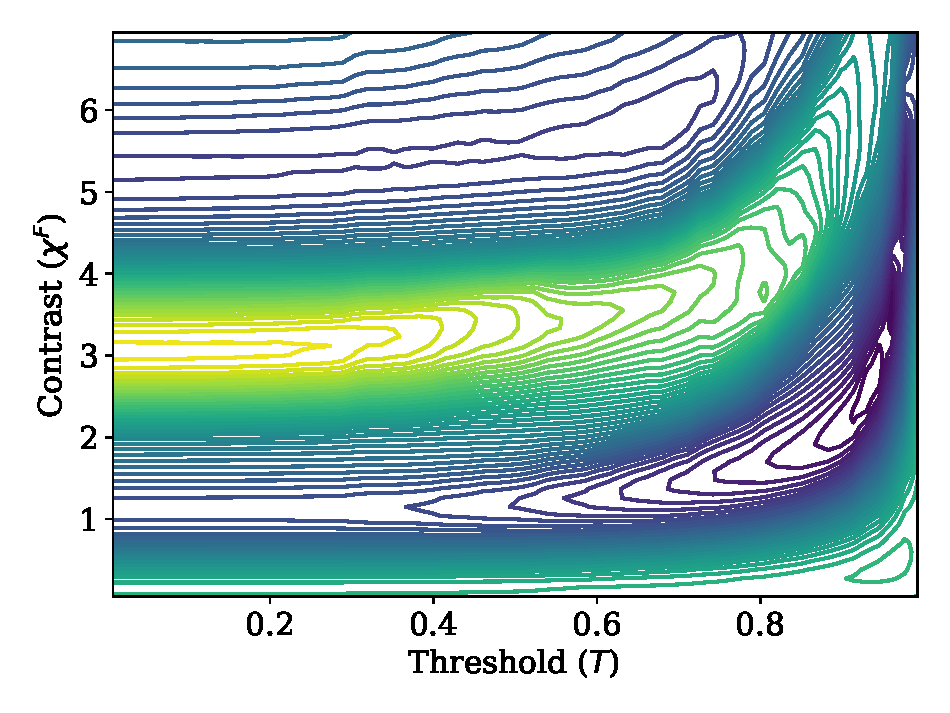
\includegraphics[width=.4\textwidth]{./figuras/samplings_objfun}\label{fig:proposed-methodology:surrogate:algorithms:samplings:objfun}} \\
				\subfloat[]{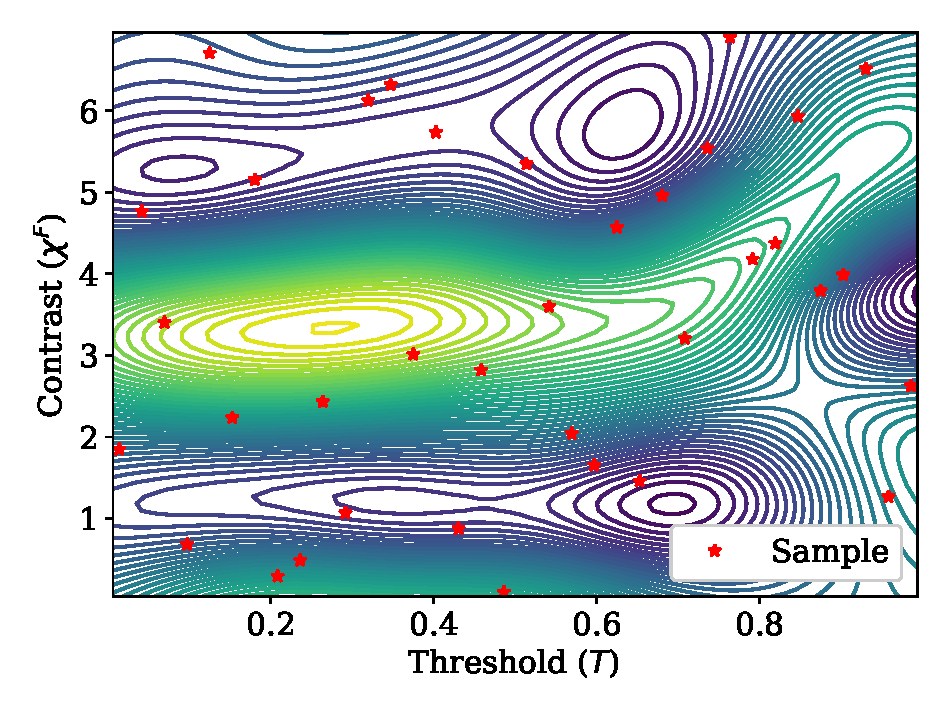
\includegraphics[width=.4\textwidth]{./figuras/samplings_lhs}\label{fig:proposed-methodology:surrogate:algorithms:samplings:lhs}} \hspace{.1\textwidth}
				\subfloat[]{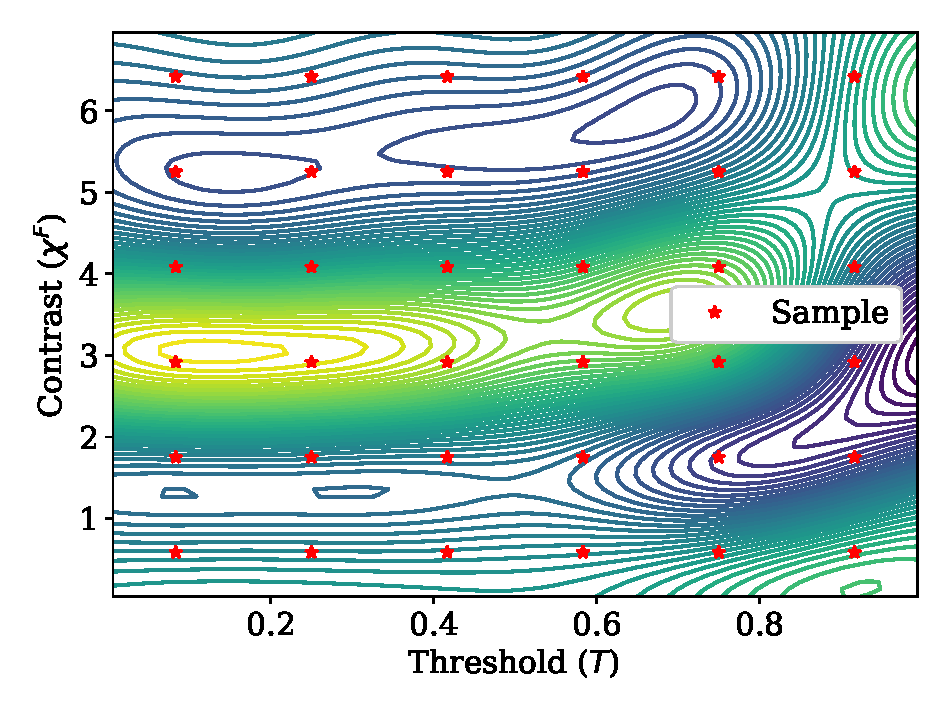
\includegraphics[width=.4\textwidth]{./figuras/samplings_uniform}\label{fig:proposed-methodology:surrogate:algorithms:samplings:uniform}}
				\caption[Comparison of Latin Hypercube Sampling and Uniform Sampling methods for strong scatterer instance.]{Comparison of Latin Hypercube Sampling and Uniform Sampling methods for strong scatterer instance: (a) the ground-truth image; (b) the surface of the corresponding objective-function; (c) the predicted surface obtained by LHS; (d) the predicted surface obtained by uniform sampling.}
				\label{fig:proposed-methodology:surrogate:algorithms:samplings}
			\end{figure}
			
			Surrogate Model-Assisted Evolutionary Algorithms (SAEAs) are a popular approach  \citep{emmerich2006single,liu2014gaussian}. Despite the various possible formulations of SAEAs \citep{buche2005accelerating}, they all share the same general structure \citep{he2023review}. In Figure \ref{fig:proposed-methodology:surrogate:algorithms:saeaflowchart}, the general flowchart is illustrated. The main cycle of the algorithm is initiated after the initial set of solutions is obtained and the surrogate model is built. In each generation of the cycle, the current surrogate-model is utilized to evaluate the fitness values of individuals instead of the real objective-function. An evolutionary algorithm is then employed to continually search for the optimal solution of the problem. Meanwhile, high-quality individuals are selected to update the sample and, therefore, are evaluated according the true objective function to update the surrogate-model \citep{zhou2007combining,liu2014gaussian,sun2017surrogate}. These operations are repeated until the termination condition is met \citep{jin2005comprehensive}.
			
			\begin{figure}[!h]
				\centering
				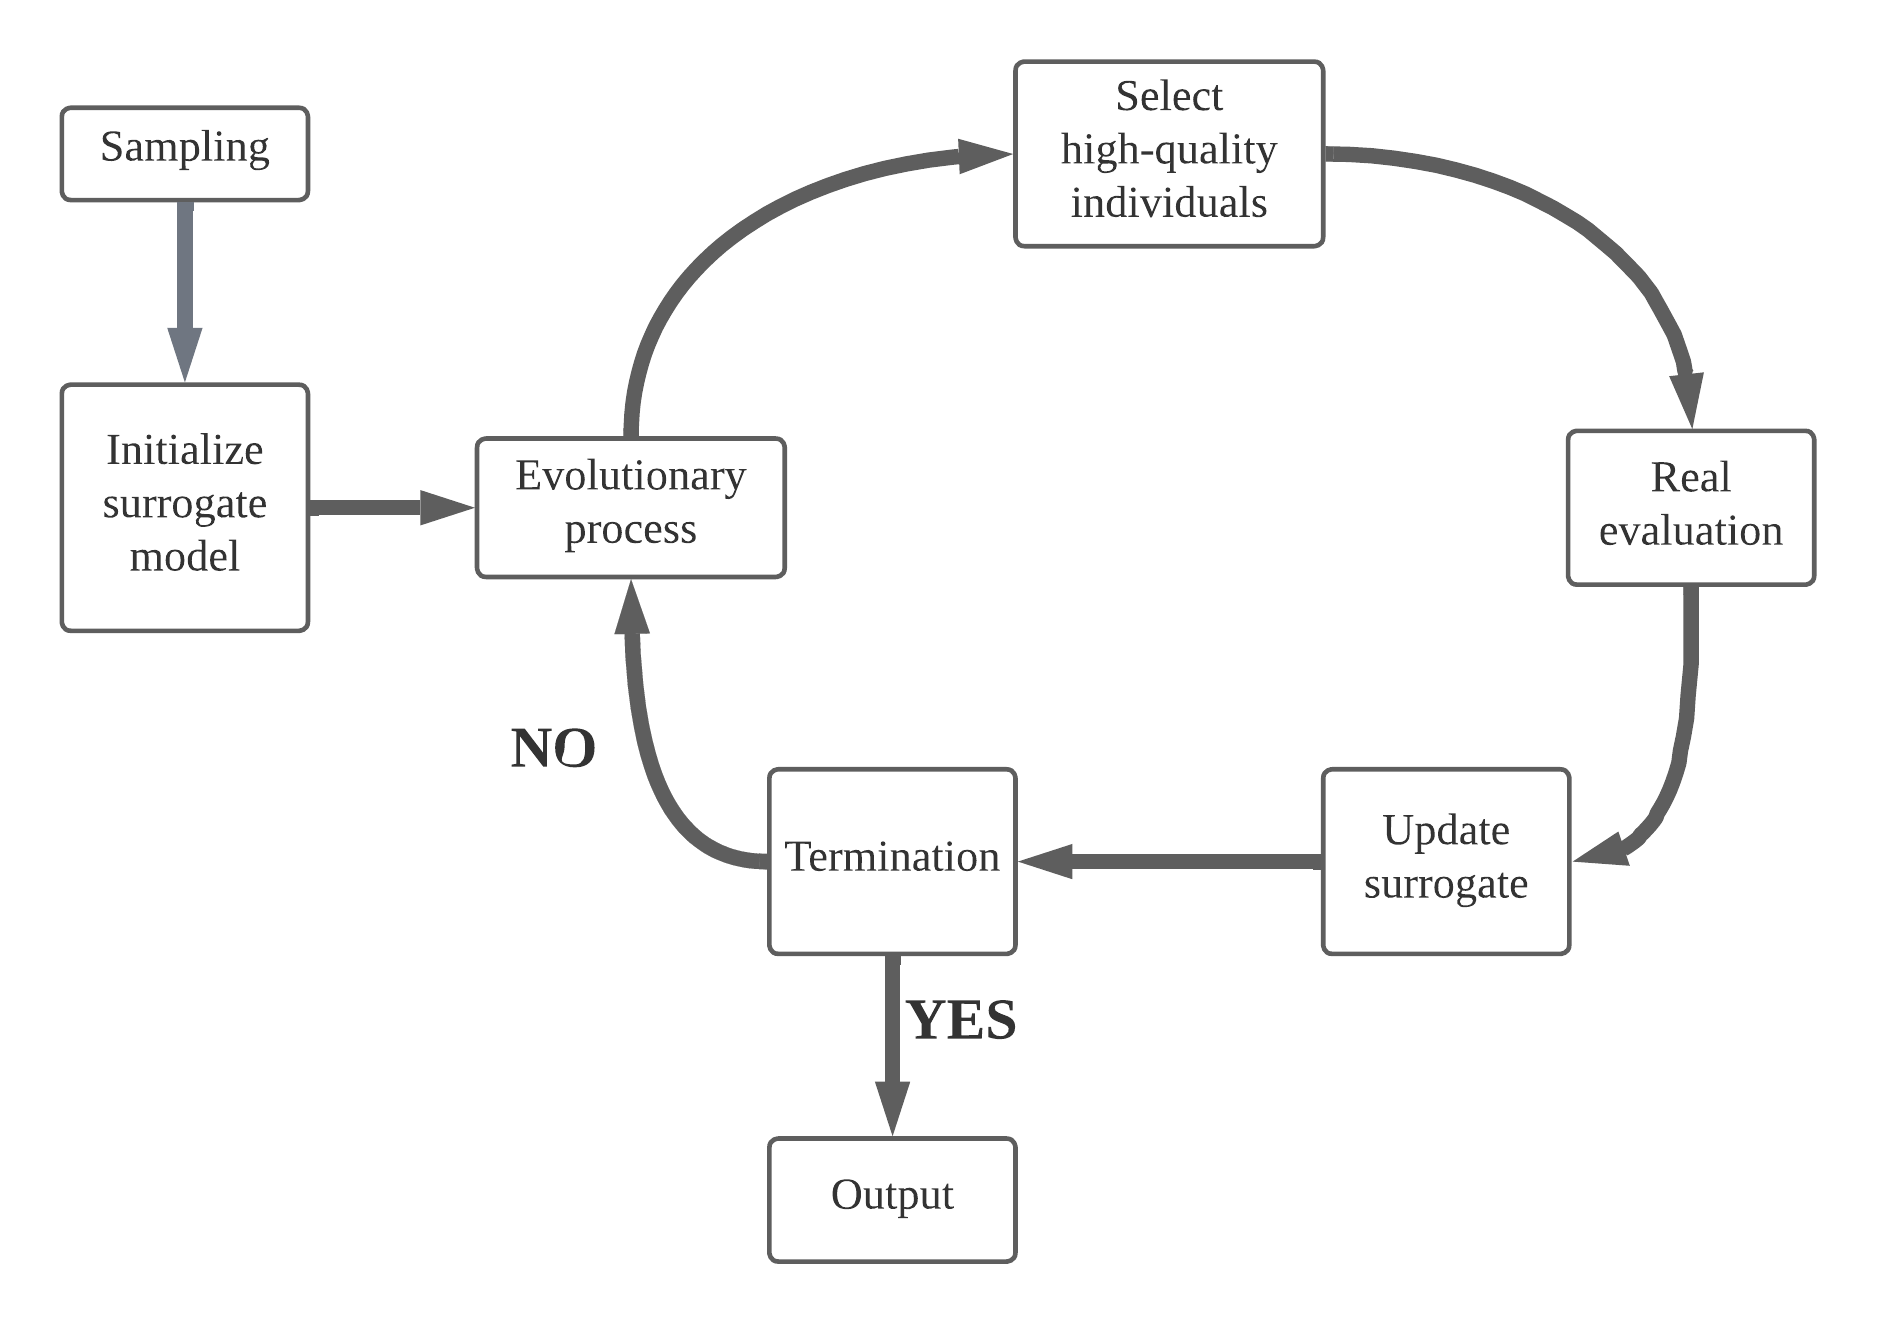
\includegraphics[width=.8\textwidth]{./figuras/saeaflowchart}
				\caption[The basic flowchart of SAEAs.]{The basic flowchart of SAEAs.}
				\label{fig:proposed-methodology:surrogate:algorithms:saeaflowchart}
			\end{figure}
			
			In surrogate model-assisted optimization algorithms, it is not only population-based algorithms that can be used. Since the surrogate model is constructed from smooth basis functions, it is also possible to use search direction methods based on derivatives. Once the surrogate model is built, a local optimum of the predicted surface can be obtained by applying such methods to a given starting point. This local optimum is then evaluated based on the true objective function, and the surrogate model is updated with this new sample. This process is then repeated with the final solution from the previous iteration as the new starting point. Given that the objective function is reasonably sampled early on, such a method could converge to the optimum solution. A stopping criterion for this method could be consecutive iterations in which the optimal solution does not change. Different formulations can be explored for choosing the first starting point of the search direction method. This can be especially important in multimodal problems, such as the one addressed in this thesis.
		
			In this thesis, three SAEAs approaches are considered. Their differences are the way in which the population is initialized and the way in which the high-quality individuals are selected for updating the model. In addition, two Surrogate model-Assisted Descent Methods (SADMs) are also proposed. Their main difference is the approach for obtaining an initial solution. The next subsubsections describe all of them.
		
			\subsubsection{SAEA1}\label{chap:proposed-methodology:surrogate:algorithms:saea1}
			
				The first SAEA approach is inspired in \citep{salucci2022learned}. After initializing the surrogate model, the population is initialized by simply sampling random points in the search space following the uniform distribution. Their fitness are computed by the surrogate model prediction. Then, the algorithm executes a single iteration of the chosen evolutionary process. After the new population is selected\footnote{The elitism strategy is considered, i.e., the best solution among the parent and offspring populations is preserved for the next generation.}, the current best solution is compared against the sample. If it differs from all available solutions in the sample, its fitness is updated according to the real objective function and it is added to the sample. The model is trained again and all the individuals in the current population are re-evaluated according the updated surrogate model. The cycle repeats and this process continues until the stop criterion is met, at which point the algorithm returns the best solution in the sample. The pseudo-code presented in Algorithm \ref{alg:saea1} outlines this process.
				
				Overall, the following observations are drawn for the considered algorithm:
				\begin{itemize}
					\item The sample contains the initial solution and the best individuals discovered throughout the generations.
					\item The total number of evaluations of the true objective function is not greater than the sum of the number of initial samples and the number of generations.
					\item The offspring population is created using the DE/best/1 operator, and the F factor is randomly selected from a predetermined range.
					\item In addition, a local search step based on a Descent Method is added and performed after a fixed number of generations, which distinguishes this process from the one proposed by \cite{salucci2022learned}.
				\end{itemize}
				
				\begin{algorithm}[!h]
					\caption[Explanation of the functioning of the SAEA1 algorithm.]{The SAEA1 algorithm.}
					\label{alg:saea1}
					\KwIn{Scattered field data, discretization configuration, lower and upper bounds for $\chi^F$ and $T$, number of initial sampled solutions, population size}
					\KwOut{Contrast image.}
					Solve qualitatively the problem and obtain the normalized contrast image.\\
					Sample solutions within the search space uniformly in the defined interval of $\chi^F$ and $T$.
					Evaluate the sampled solutions.\\
					Evaluations $\leftarrow$ number of initial sampled solutions.\\
					Build and train the surrogate model based on the sample.\\
					Initialize a population of individuals by randomizing $\chi^F$ and $T$ values following the uniform distribution.\\
					Set their fitness according to their corresponding prediction obtained by the surrogate model.\\
					\While{stopping criteria is not met}{
						Generate a offspring population based on the DE/best/1 operator.\\
						Evaluate the offspring based on the surrogate model.\\
						Selected the new population considering the union of parents and offspring individuals by Binary Tournament and preserving the best solution among them (elitism).\\
						\If{the local search has not been executed in the last $N_{LS}$ generations}{
							Perform a local search using a Steepest Descent algorithm considering the current best solution as initial guess and the surrogate model as objective function.\\
							\If{the returned solution by the local search is better}{
								Update the current best solution.\\
							}	
						}
						\If{the current best solution is not equal to any other in the sample}{
							Evaluate the current best solution according the objective function.\\
							Evaluations $\leftarrow$ evaluations + 1\\
							Add the current best solution to the sample.\\
							Train the surrogate model.\\
							Re-evaluate the population using the updated surrogate model.\\
						}
					}
				\end{algorithm}
			
			\subsubsection{SAEA2}\label{chap:proposed-methodology:surrogate:algorithms:saea2}
				
				The second approach is inspired in the one proposed by \cite{valadao2020comparative}. The approach for selection and mutation in this algorithm differs from the typical prediction model-based population evaluation implemented in SAEA1. Instead, individual evaluation using the real function serves as the criterion for selection. The mutation strategy is also distinct, with mutation vectors calculated based on solutions stored in an archive. The archive is initially populated with the best solutions from the samples and is updated in each generation with the best $N_A$ solutions from the updated sample. Each offspring-individual is generated from a sub-selection of solutions, generated and evaluated by the surrogate model. The sub-selection generates a set of solutions, and the one with the best value for the prediction of the objective function is selected as the offspring. Then, its fitness is updated according the real objective function. The pseudo-code presented in Algorithm \ref{alg:saea2} outlines this process.
				
				In practice, the described algorithm leads to the following observations:
				\begin{itemize}
					% \item A amostra de soluções é sempre atualizada com as melhores soluções encontradas até geração atual. Logo, soluções com avaliaçõs ruins são retiradas de modo que o modelo prioriza mais a reconstrução da região mais promissora.
					\item The sample solutions are continuously updated with the best solutions found up to the current generation. This means that sampled solutions with the worst evaluations are removed to prioritize the reconstruction of the most promising region.
					% \item A cada geração, o número de avaliações aumenta com o tamanho da população. Portanto, este algoritmo tende a gastar mais avaliações para convergir.
					\item The number of evaluations increases with each generation in proportion to the population size, causing this algorithm to require more evaluations to converge.
					% \item Os mesmos operadores de mutação e de busca local foram aplicados nesta versão do algoritmo.
					\item The current version of the algorithm applies the same mutation and local search operators in each iteration.
				\end{itemize}
    
				\begin{algorithm}[!h]
					\caption[Explanation of the functioning of the SAEA2 algorithm.]{The SAEA2 algorithm.}
					\label{alg:saea2}
					\KwIn{Scattered field data, discretization configuration, lower and upper bounds for $\chi^F$ and $T$, number of initial sampled solutions, population size}
					\KwOut{Contrast image.}
					Solve qualitatively the problem and obtain the normalized contrast image.\\
					Sample solutions within the search space uniformly in the defined interval of $\chi^F$ and $T$.
					Evaluate the sampled solutions.\\
					Evaluations $\leftarrow$ number of initial sampled solutions.\\
					Build and train the surrogate model based on the sample.\\
					Initialize a population of individuals by selecting the $p$ best solutions from the sample.\\
					Store in the archive the best $N_A$ solutions.\\
					\While{stopping criteria is not met}{
						Generate $k$ solutions for each one in the population based on the DE/best/1 operator and evaluate them according to the surrogate model.\\
						For each group of $k$ solutions, selects the best, evaluate it according to the real function and set it as offspring individual.\\
						Evaluations $\leftarrow$ evaluations $+$ population size.\\
						Selected the new population considering the union of parents and offspring individuals by Binary Tournament and preserving the best solution among them (elitism).\\
						\If{the local search has not been executed in the last $N_{LS}$ generations}{
							Perform a local search using a Steepest Descent algorithm considering the current best solution as initial guess and the surrogate model as objective function.\\
							\If{the returned solution by the local search is better}{
								Update the current best solution.\\
							}	
						}
						\If{the current best solution is not equal to any other in the sample}{
							Add the current best solution to the sample.\\
							Train the surrogate model.\\
						}
						Update the archive with the $N_A$ best solutions in the sample.\\
					}
				\end{algorithm}
	
			\subsubsection{SAEA3}\label{chap:proposed-methodology:surrogate:algorithms:saea3}
			
				% A principal vantagem do SAEA1 é gastar somente uma avaliação por geração. Já a principal do SAEA2 é considerar um arquivo de melhores soluções como indivíduos-pais no momento da mutação. Estas duas características podem ser combinadas numa formulação híbrida, a SAEA3, na qual a população de indivíduos pais e filhos continua sendo avaliada pelo modelo substituto, ao passo que os vetores de mutação são gerados considerando um arquivo com as melhores soluções da amostra. Dessa forma, apenas a melhor solução da geração é avaliada pela função real. Desta forma, um número alto de gerações que o SAEA2 pode ser considerado e os indivíduos filhos tendem a herdar mais características das melhores soluções.
				SAEA1 has the main advantage of spending only one evaluation per generation, while SAEA2 has the advantage of considering an archive of best solutions as parents during mutation. The features of these two algorithms can be combined in a hybrid formulation, called SAEA3, where the population of parent and offspring individuals is evaluated by the surrogate model, and mutation vectors are generated based on a file with the best sample solutions. As a result, only the best solution of the generation is evaluated by the actual function. This approach enables SAEA3 to have a high number of generations, similar to SAEA1, while the offspring individuals tend to inherit more characteristics of the best solutions (exploitation), similar to SAEA2. The same mutation and local search operators in each iteration. The pseudo-code presented in Algorithm \ref{alg:saea3} outlines this process.
				
				\begin{algorithm}[!h]
					\caption[The SAEA3 algorithm.]{Explanation of the functioning of the SAEA3 algorithm.}
					\label{alg:saea3}
					\KwIn{Scattered field data, discretization configuration, lower and upper bounds for $\chi^F$ and $T$, number of initial sampled solutions, population size}
					\KwOut{Contrast image.}
					Solve qualitatively the problem and obtain the normalized contrast image.\\
					Sample solutions within the search space uniformly in the defined interval of $\chi^F$ and $T$.
					Evaluate the sampled solutions.\\
					Evaluations $\leftarrow$ number of initial sampled solutions.\\
					Build and train the surrogate model based on the sample.\\
					Initialize a population of individuals by selecting the $p$ best solutions from the sample.\\
					Store in the archive the best $N_A$ solutions.\\
					\While{stopping criteria is not met}{
						Generate $k$ solutions for each one in the population based on the DE/best/1 operator and evaluate them according to the surrogate model.\\
						For each group of $k$ solutions, selects the best and set it as offspring individual.\\
						Selected the new population considering the union of parents and offspring individuals by Binary Tournament and preserving the best solution among them (elitism).\\						
						\If{the local search has not been executed in the last $N_{LS}$ generations}{
							Perform a local search using a Steepest Descent algorithm considering the current best solution as initial guess and the surrogate model as objective function.\\
							\If{the returned solution by the local search is better}{
								Update the current best solution.\\
							}	
						}
						\If{the current best solution is not equal to any other in the sample}{
							Evaluate the current best solution according the objective function.\\
							Evaluations $\leftarrow$ evaluations + 1\\
							Add the current best solution to the sample.\\
							Train the surrogate model.\\
							Re-evaluate the population using the updated surrogate model.\\
						}
						Update the archive with the $N_A$ best solutions in the sample.\\
					}
				\end{algorithm}
			
			\subsubsection{SADM1}\label{chap:proposed-methodology:surrogate:algorithms:sadm1}
			
				% 1. Os algoritmos evolutivos podem explorar todo o espaço de busca, uma vez que são baseados em uma população de soluções.
				% 2. Quando um operador de busca local é aplicado sobre a atual melhor solução, o desempenho pode melhorar uma vez que se realiza uma busca mais intensa sobre uma solução potencial.
				% 3. O processo de amostragem do espaço de busca feito para construir o modelo substituto inicial pode ser pensado como uma população de soluções. Desta forma, se essa amostragem for razoavelmente ampla, a bacia de atração com maior potencial tem boas chances de ser amostrada. Nessas condições, podemos aplicar diferentes estratégias para escolher um ponto inicial e aplicar um algoritmo de direção de busca sobre o modelo substituto.
				% 4. Obviamente, a melhor solução encontrada pode não estar tão próxima do ótimo global. No entanto, esta pode ser avaliada de acordo com a função real e adicionada ao conjunto de amostras para atualizar o modelo.
				% 5. Logo, se esse processo for repetido iterativamente, o algoritmo tenderá a convergir para um local quando a soluções ótimas encontradas em um conjunto de iterações forem idênticas ou muito próximas.
				% 6. A grande questão é então como escolher a solução inicial que vai dar início ao processo iterativo de otimização.
				% 7. Uma possível estratégia é executar um algoritmo evolutivo considerando o modelo substituto inicial e tomar como solução inicial do processo iterativo a melhor solução encontrada pelo algoritmo evolutivo. Assim, uma busca global é feita e o processo iterativo tende a se concentrar na região da melhor bacia de atração disponível na primeira construção do modelo.
				
				Evolutionary algorithms are powerful optimization techniques based on a population of solutions. They are capable of exploring the entire search space (exploration), and when combined with local search operators, performance can improve significantly due to the exploitation of a potential solution. The initial surrogate model construction can be seen as a population of solutions, which, if sampled broadly, can cover the most promising region of the search space. Different strategies can be applied to choose a starting point and apply a steepest descent algorithm on the surrogate model.
				
				The best solution found may not necessarily be close to the global optimum, but it can be evaluated against the actual function and added to the sample set to update the model. By repeating this process iteratively, the algorithm will tend to converge to a location when the optimal solutions found in a set of iterations are identical or very close. However, the question of how to choose the initial solution that will start the iterative optimization process remains.
				
				One possible strategy is to run an evolutionary algorithm considering the initial surrogate model and take the best solution found as the initial solution of the iterative process. This way, a global search is performed, and the iterative process tends to focus on the region of the best basin of attraction available in the first construction of the model. Such an approach will be denoted as SADM1 where the initials stand for Surrogate-model Assisted Descent Method. The pseudo-code presented in Algorithm \ref{alg:sadm1} outlines this process.
				
				Overall, the following observations are drawn for the considered algorithm:
				\begin{itemize}
					\item The evolutionary algorithm employed to determine an initial guess is the Differential Evolution with the following formulation: DE/best/1/bin \citep{rocca2011differential}.
					\item The employed descent method is the L-BFGS-B algorithm which is a limited-memory version of Broyden-Fletcher-Goldfarb-Shanno (BFGS) algorithm for boundary constrained optimization \citep{byrd1995limited,zhu1997algorithm}.
				\end{itemize}
				
				\begin{algorithm}[!h]
					\caption[Explanation of the functioning of the SADM1 algorithm.]{The SADM1 algorithm.}
					\label{alg:sadm1}
					\KwIn{Scattered field data, discretization configuration, lower and upper bounds for $\chi^F$ and $T$, number of initial sampled solutions, population size}
					\KwOut{Contrast image.}
					Solve qualitatively the problem and obtain the normalized contrast image.\\
					Sample solutions within the search space uniformly in the defined interval of $\chi^F$ and $T$.
					Evaluate the sampled solutions.\\
					Evaluations $\leftarrow$ number of initial sampled solutions.\\
					Build and train the surrogate model based on the sample.\\
					Run an evolutionary algorithm considering the surrogate model as objective function and take the best solution as current solution.\\
					Evaluate the current solution according the true objective function, add it to the sample and retrain the model.\\
					\While{stopping criteria is not met}{
						Run the descent method considering the current solution as initial guess and optimizing the predicted surface.\\
						Evaluate the returned solution according the true objective function.\\
						Evaluations $\leftarrow$ evaluations + 1\\
						\If{the returned solution is not equal to any other in the sample}{
							Add the current best solution to the sample.\\
							Train the surrogate model.\\
						}
						\If{the returned solution is better than the current one}{
							Set the current solution as the returned by the last call of the descent optimization.\\
						}
					}
				\end{algorithm}
	
			\subsubsection{SADM2}\label{chap:proposed-methodology:surrogate:algorithms:sadm2}
			
				% 1. Ao invés de determinar o ponto inicial para o processo iterativo do SADM através da utilização de um algoritmo evolucionário, uma alternativa mais simples é escolher a melhor amostra como ponto de partida. Ou seja, após amostrar o espaço de busca, o processo iterativo começa assumindo como solução atual a melhor amostra do modelo.
				% 2. Além de mais simples, uma vantagem é evitar a possibilidade de convergir para uma outra bacia de atração diferente da de mínimo global quando esta estiver perto da melhor amostra. Em outras palavras, considerando a superfície gerada pelo modelo substituto, o algoritmo evolutivo não garante a convergência para o mínimo globa, uma vez que é estocástico. No entanto, se por um acaso o mínimo global estiver próximo da melhor amostra, o que é bem possível, então a primeira iteração do SADM convergirá para esse local.
				% 3. É claro que, se a superfície não for bem amostrada no começo, então poder ser o processo convirja para uma região diferente da do ótimo global da função real. E isso pode ser mais complicado em casos de espalhadores fortes, onde a função objetivo tende a ser multi-modal. Mas quando a função objetivo é menos complexa, então essa estratégia pode ser bem eficiente.
				
				Rather than determining the starting point for the SADM iterative process using an evolutionary algorithm, a simpler alternative is to choose the best sample as the starting point. That is, after sampling the search space, the iterative process starts assuming the best sample of the model as the current solution. In addition to being simpler, an advantage is to avoid the possibility of converging to another basin of attraction different from the global minimum when this is close to the best sample. In other words, considering the surface generated by the surrogate model, the evolutionary algorithm does not guarantee convergence to the global minimum, since it is stochastic. However, if by chance the global minimum is close to the best sample, which is quite possible, then the first iteration of SADM will certainly converge to that location. Of course, if the surface is not sampled well at the beginning, then the process may converge to a region other than the global optimum of the real function. And this can be more complicated in cases of strong scatterers, where the objective function tends to be multi-modal. But when the objective function is less complex then this strategy can be quite efficient. This approach will be denoted as SADM2 and its pseudo-code is shown in Algorithm \ref{alg:sadm2}. The L-BFGS-B algorithm will be used in a similar manner to SADM1.
				
				\begin{algorithm}[!h]
					\caption[Explanation of the functioning of the SADM2 algorithm.]{The SADM2 algorithm.}
					\label{alg:sadm2}
					\KwIn{Scattered field data, discretization configuration, lower and upper bounds for $\chi^F$ and $T$, number of initial sampled solutions, population size}
					\KwOut{Contrast image.}
					Solve qualitatively the problem and obtain the normalized contrast image.\\
					Sample solutions within the search space uniformly in the defined interval of $\chi^F$ and $T$.
					Evaluate the sampled solutions.\\
					Evaluations $\leftarrow$ number of initial sampled solutions.\\
					Build and train the surrogate model based on the sample.\\
					Set the best sample as the current solution.\\
					\While{stopping criteria is not met}{
						Run the descent method considering the current solution as initial guess and optimizing the predicted surface.\\
						Evaluate the returned solution according the true objective function.\\
						Evaluations $\leftarrow$ evaluations + 1\\
						\If{the returned solution is not equal to any other in the sample}{
							Add the current best solution to the sample.\\
							Train the surrogate model.\\
						}
						\If{the returned solution is better than the current one}{
							Set the current solution as the returned by the last call of the descent optimization.\\
						}
					}
				\end{algorithm}
	
	\section{EISPY2D: A Platform for Developing and Testing Algorithms for EISPs}\label{chap:proposed-methodology:library}
		
		This section presents the proposed framework for the development and testing of algorithms for the electromagnetic inverse scattering problem. The framework is a Python package with implemented classes that provide a structured environment for algorithm development and testing. The novelty of the proposed framework lies in three key aspects. Firstly, it includes the collection of indicators with the proposal of two specific metrics that allow for a comprehensive evaluation of the algorithms' performance. Secondly, the framework proposes an approach to test randomization, which ensures a fairer and more reliable comparison between algorithms. Finally, a statistical routine based on traditional statistical tests is proposed to compare the algorithms' performance. This section provides a brief description of the proposed framework and its features, highlighting the significance and contribution of each aspect.
		
		\subsection{Structure Description}\label{chap:proposed-methodology:library:performance}

			%Para poder comparar algoritmos, foi necessário desenvolver uma plataforma comum para as implementações. Esta plataforma foi desenvolvida em forma de uma biblioteca programada na linguagem Python3  \citep{python3}. Com uma estrutura baseada em orientação a objeto, a biblioteca implementa o problema bidimensional com as configurações de domínio definidas da Seção \ref{chap:methods:definition}. Por isso, ela foi batizada como \textit{eispy2d}. O diagrama de classes UML pode ser visualizado na \autoref{fig:4:eispy2d}.
			In order to be able to compare algorithms, it was necessary to develop a common platform for the implementations. This platform was developed as a library programmed in the Python3 language \citep{vanrossum2010python}. With a structure based on object orientation, the library implements the two-dimensional problem with the domain configurations defined in Section \ref{chap:methods:definition}. Therefore, it was named \textit{eispy2d}. The UML class diagram can be seen in \autoref{fig:4:eispy2d}.
			%\begin{figure}[p]
			%	\centering
			%	\hspace*{-1in}
			%	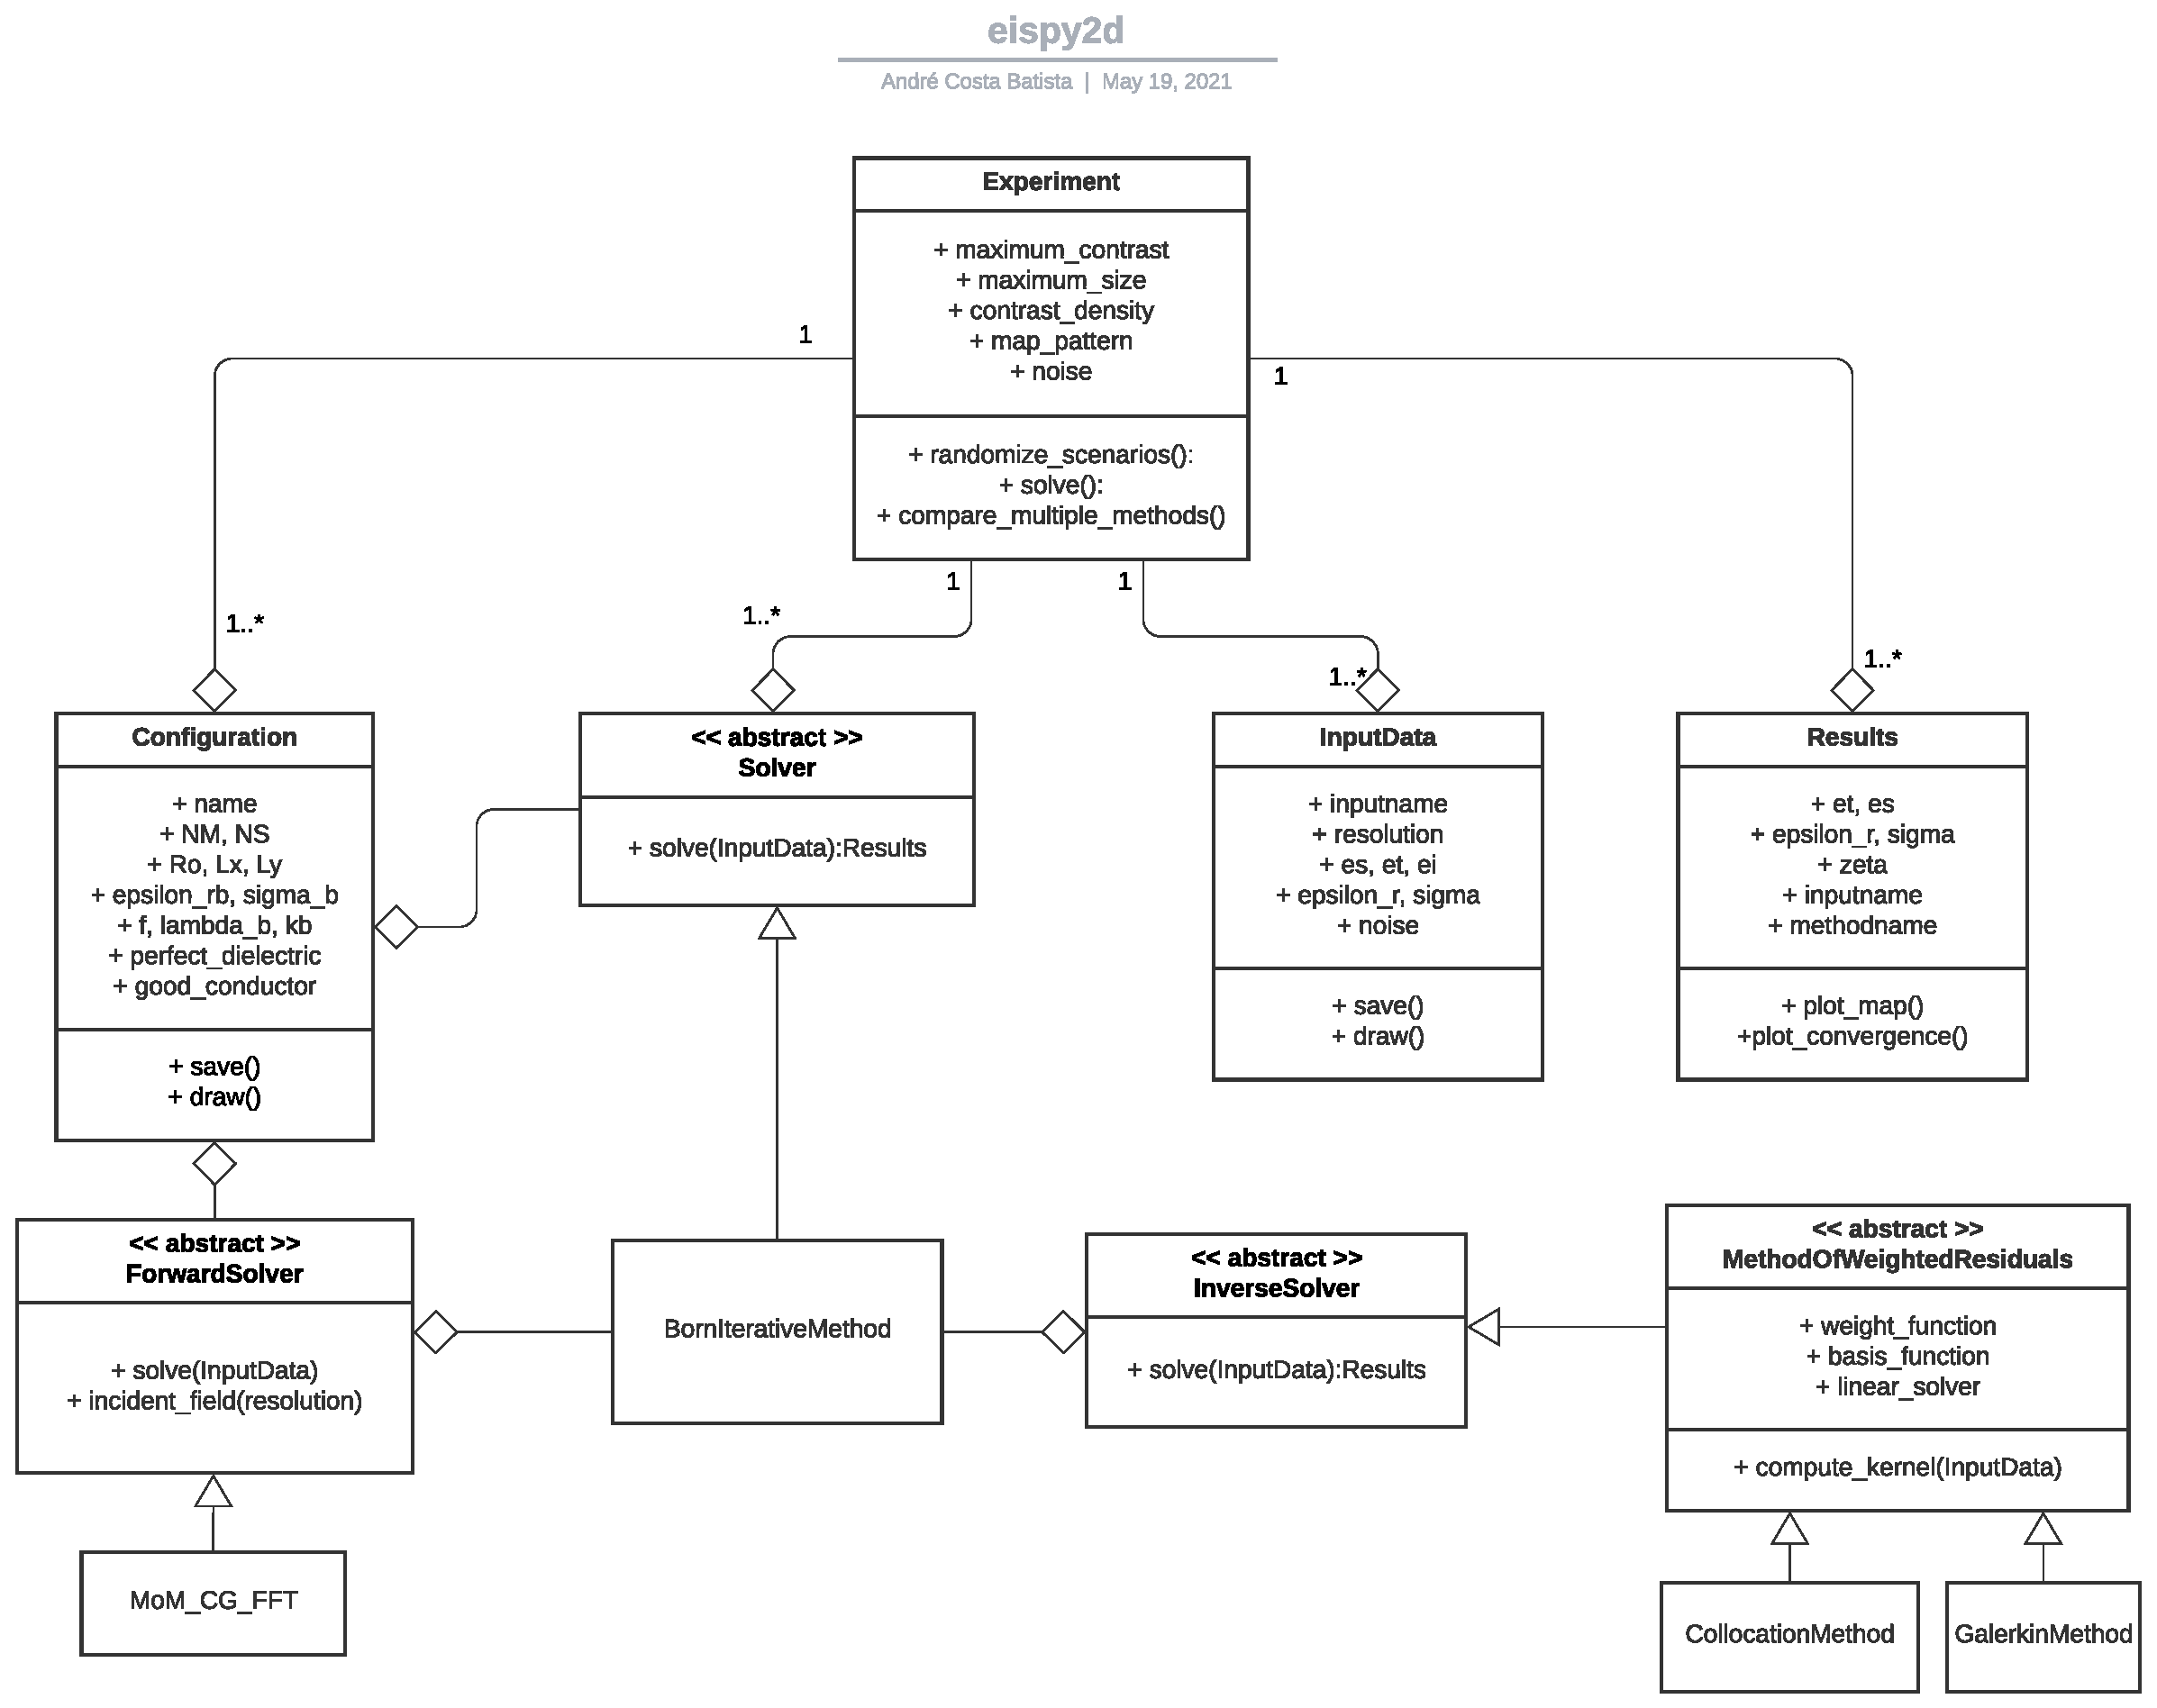
\includegraphics[width=.95\paperwidth, angle=90]{./figuras/eispy2d.eps}
			%	\vspace*{0.2in}
			%	\caption{UML Class Diagram of \textit{eispy2d} library.}
			%	\label{fig:4:eispy2d}
			%\end{figure}
			\begin{figure}[!h]
				\centering
				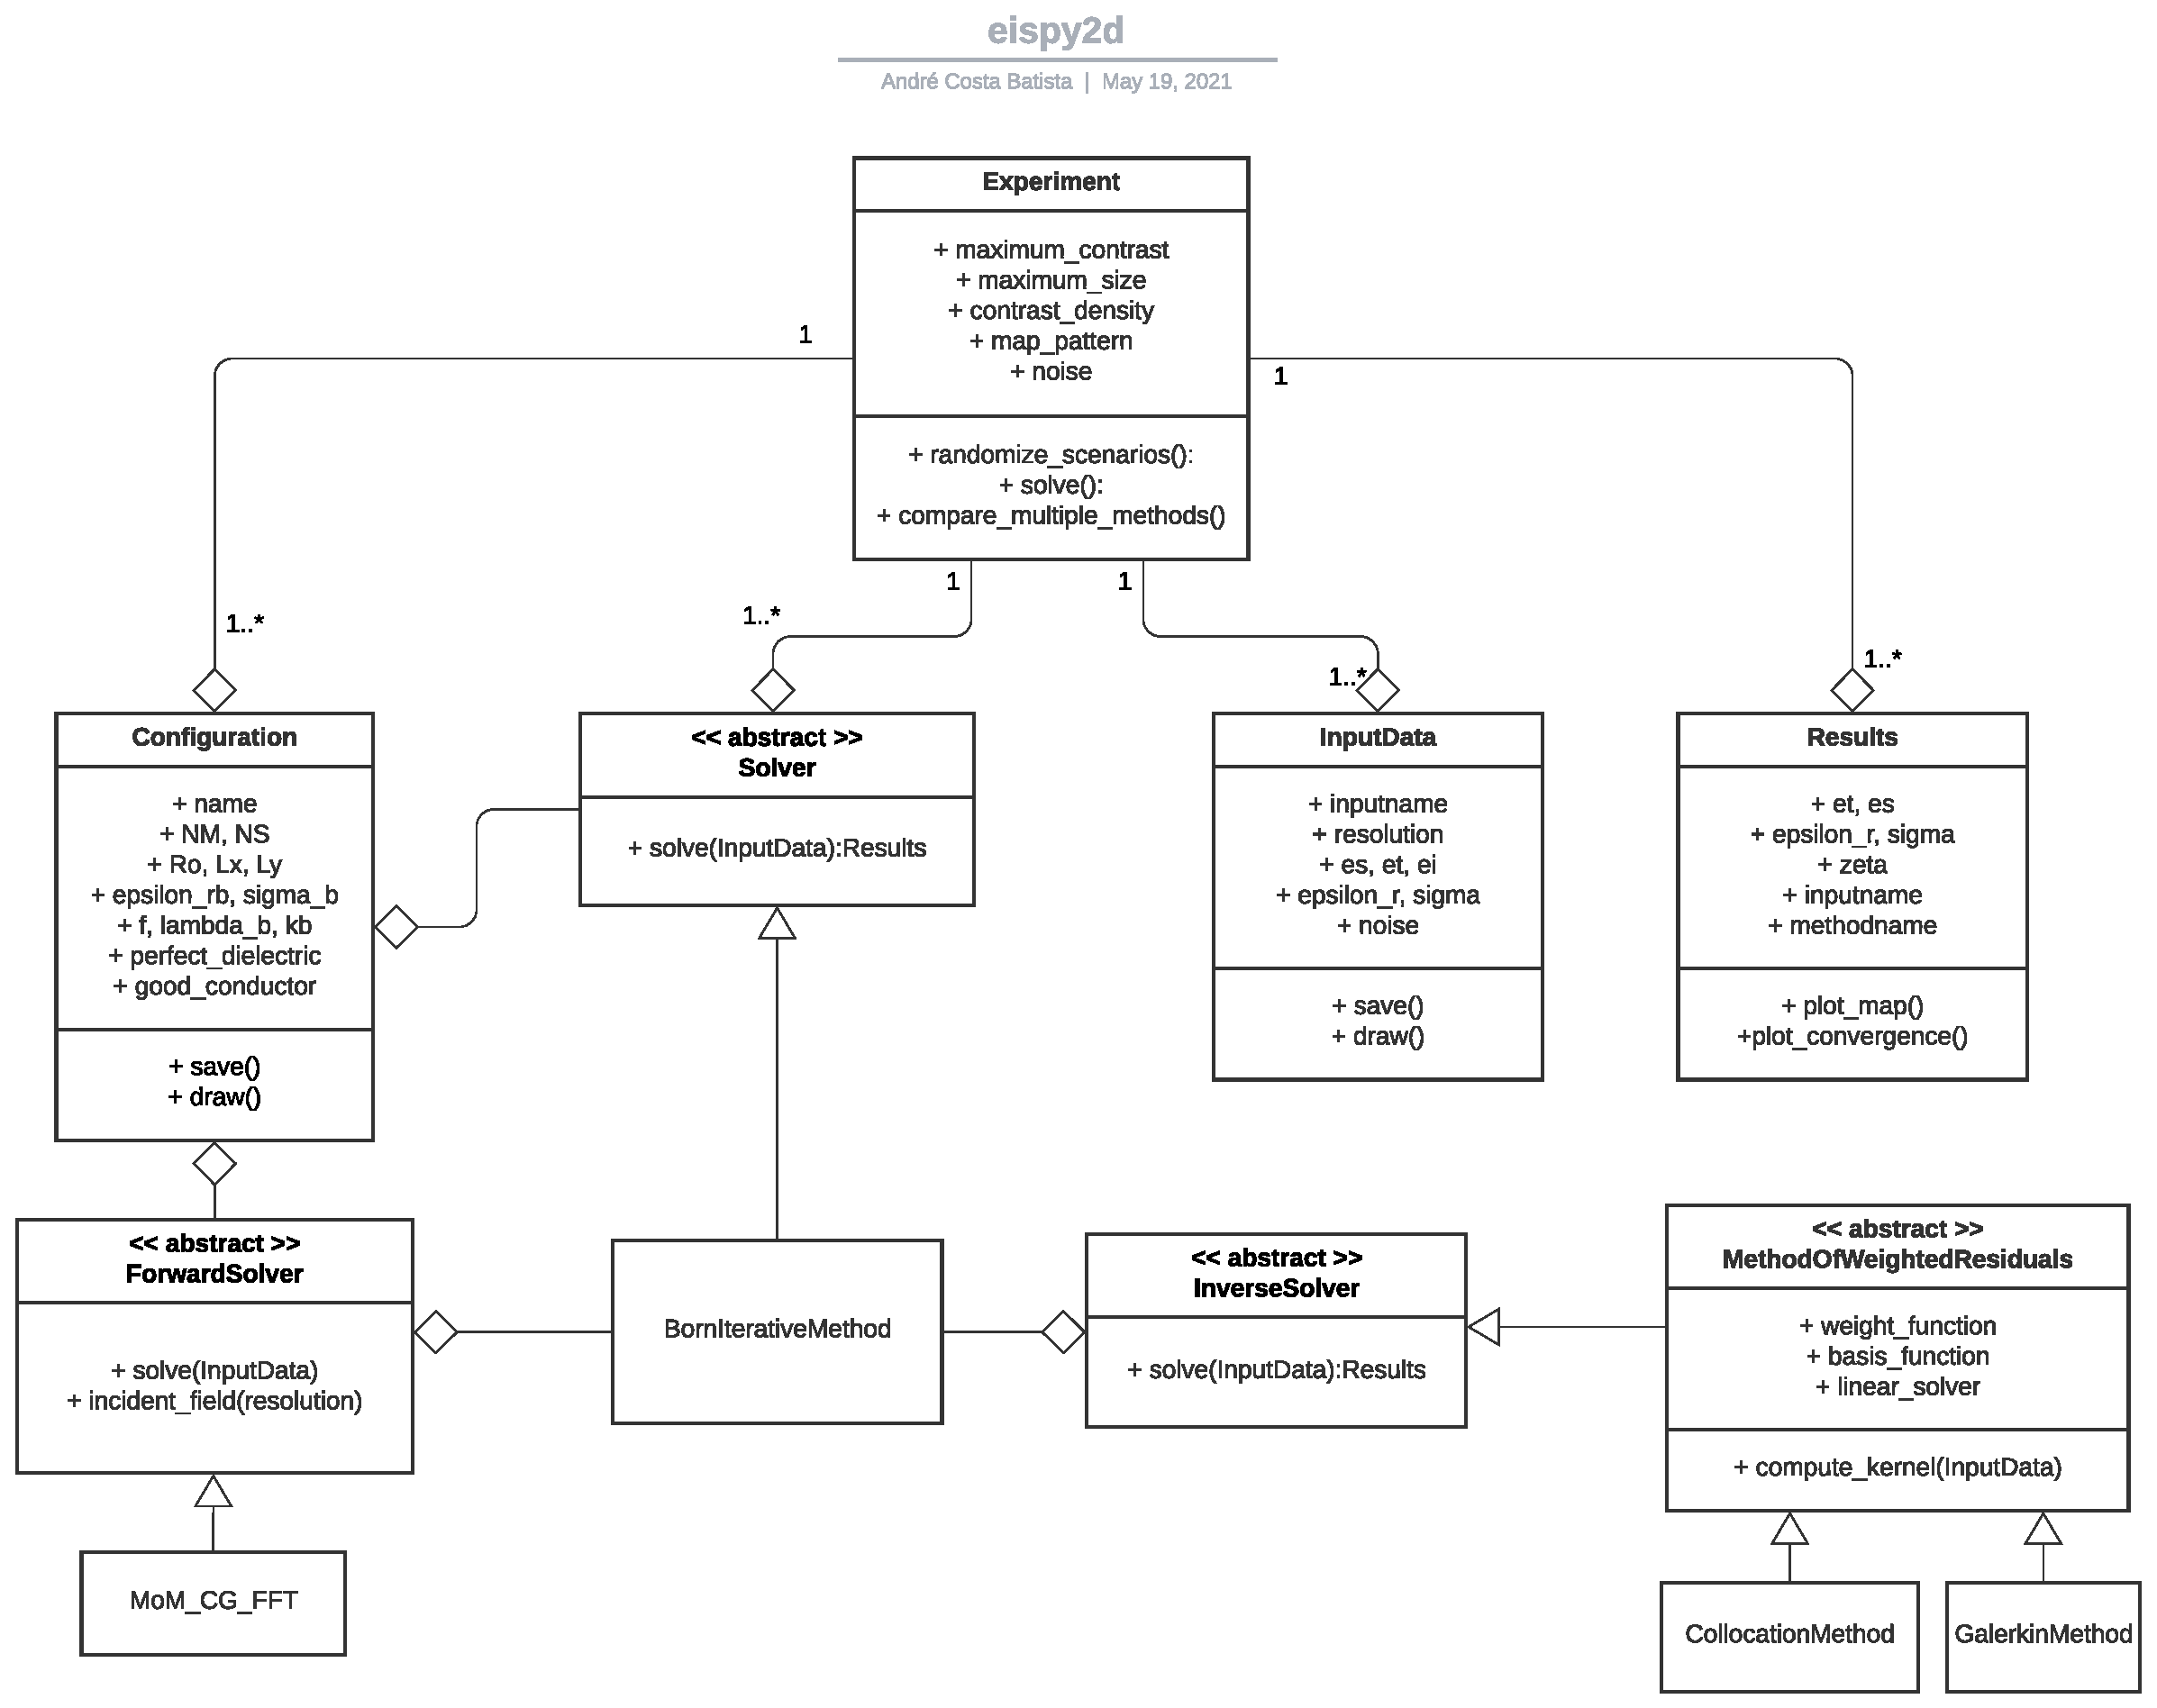
\includegraphics[width=\textwidth]{./figuras/eispy2d.eps}
				\caption[UML Class Diagram of \textit{eispy2d} library.]{UML Class Diagram of \textit{eispy2d} library.}
				\label{fig:4:eispy2d}
			\end{figure}
			
			%A seguir, uma breve explicação das classes principais:
			The following is a brief explanation of the main classes:
			\begin{enumerate}
				%\item\textbf{Configuration}: classe que guarda as informações principais do problema, como tamanho da imagem ($L_X$, $L_Y$), raio de observação ($R_O$), número de medições e de incidências ($N_M$, $N_S$);
				\item\textbf{Configuration}: a class that stores the primary information of the problem, such as image size ($L_X$, $L_Y$), observation radius ($R_O$), number of measurements and incidences ($N_M$, $N_S$);
				%\item\textbf{InputData}: classe que caracteriza uma instância de problema. Sua informação principal são os dados do campo espalhado. No entanto pode agregar outras informações como o campo total (para o problema linear) ou as imagens de contraste (para medição do erro);
				\item\textbf{InputData}: a class that characterizes a problem instance. Its primary information is the data of the scattered field. However, other information can be added, such as the total field (for the linear problem) or the contrast images (for error measurement);
				%\item\textbf{Results}: classe que guarda e exibe os resultados de uma execução do problema inverso não-linear. Além disso, também implementa os indicadores de qualidade;
				\item\textbf{Results}: a class that stores and displays the results of an execution of the nonlinear inverse problem. In addition, it also implements quality indicators;
				%\item\textbf{Solver}: uma classe abstrata para implementação de resolvedores do problema não-linear. Uma derivação, por exemplo, é a classe \textit{BornIterativeMethod} que implementa o correspondente método;
				\item\textbf{InverseSolver}: a abstract class for nonlinear inverse solvers implementation. For instance, inversion approaches such as the Born Iterative Method and the Subspace Optimization methods are derived classes which implement the corresponding methods.
				%\item\textbf{ForwardSolver}: classe abstrata para implementação de resolvedores diretos. Uma derivação, por exemplo, é o Método dos Momentos (\textit{MoM\_CG\_FFT});
				\item\textbf{ForwardSolver}: abstract class for implementing forward solvers. One derivation, for example, is the Method of Moments Conjugated Gradient-Fast Fourier Transform \citep{su1987calculation};
				%\item\textbf{InverseSolver}: classe abstrata para resolver o problema inverso linear. A classe \textit{MethodOfWeightedResiduals} é uma derivação ainda abstrata que serve para representar as discretizações \textit{CollocationMethod} e \textit{GalerkinMethod} e executar regularizadores como o de Tikhonov, Landweber e CG;
				\item\textbf{Discretization}: abstract class for discretization schemes. Each discretization strategy is a derived class, such as the Collocation Method (Subsection \ref{chap:methods:discretization:collocation}).
				%The \textit{MethodOfWeightedResiduals} class is a still abstract derivation that serves to represent the \textit{CollocationMethod} and \textit{GalerkinMethod} discretizations and execute regularizers such as Tikhonov, Landweber, and CG;
				%\item\textbf{Experiment}: classe que representa um experimento. É responsável por criar um conjunto de testes sintéticos aleatórios, executar os algoritmos e comparar resultados. Seus atributos principais são os parâmetros que configuram o conjunto de teste, i.e., o padrão de espalhado (geometrias tradicionais, aleatórias ou superfícies), o contraste máximo permitido, o tamanho máximo dos objetos, a densidade de contraste na imagem (quantidade de objetos na figura), entre outros.
				\item\textbf{Experiment}: an abstract class that represents an experiment. Two schemes are possible: case study and benchmark. For each corresponding class, there are appropriate methods for visualizing and comparing the results.
				\item\textbf{TestSet}: it is a class that contains a set of problem instances. There are appropriate methods for generating synthetic tests controlling multiple scatterer characteristics.
				% It is responsible for creating a set of random synthetic tests, executing the algorithms, plotting results, and comparing results. Its main attributes are the parameters that configure the test set, i.e., the scatter pattern (traditional, random, or surface geometries), the maximum allowed contrast, the maximum size of the objects, the density of contrast in the image (number of objects in the image), among others.
			\end{enumerate}

			%Para avaliar ou comparar a performance entre os algoritmos, três aspectos são fundamentais: os indicadores de qualidade, os princípios para criação de conjuntos de teste aleatórios e a metodologia de comparação. As próximas subsubseções trarão maiores explicações destes três aspectos. Cada um deles incluem tanto técnicas já conhecidas quanto novas propostas implementadas neste trabalho que a contribuição desta investigação é uma estrutura mais robusta de experimentação sintética.
			Three aspects are fundamental to evaluate or compare the performance among the algorithms: the quality indicators, the principles for creating random test sets, and the comparison methodology. The following subsections will provide further explanations of these three aspects. Each of them includes both techniques already known and newly proposed ones; therefore, this investigation's contribution is a more robust structure of synthetic experimentation.
			
		\subsection{Performance Metrics Proposal}\label{chap:proposed-methodology:library:metrics}
		
			%Um conjunto de indicadores foram implementados para a avaliar a qualidade da reconstrução feita pelos algoritmos. De maneira similar a \eqref{eq:4:error0:epsilon}, o erro percentual médio de estimação da permissividade relativa e o erro médio de estimação da condutividade serão calculados por:
			A set of indicators were implemented to assess the quality of the reconstruction done by the algorithms. The indicator were chosen according to their popularity throughout the references in the literature. The intention is also to aggregate indicators with different to enable multiple ways to analyze the performance of a method. Similar to \eqref{eq:4:error0:epsilon}, the average percentage error of estimation of relative permittivity and the average error of estimation of conductivity will be calculated by:
			\begin{align}
				\zeta_{\epsilon PAD} &= \frac{1}{N_IN_J}\sum\limits_{i=1}^{N_I}\sum\limits_{j=1}^{N_J}\left|\frac{\epsilon^*_{r,ij}-\epsilon_{r,ij}}{\epsilon^*_{r,ij}}\right|\times100~[\%/\mathrm{pixel}] \label{eq:4:zeta:epad} \\
				\zeta_{\sigma AD} &= \frac{1}{N_IN_J}\sum\limits_{i=1}^{N_I}\sum\limits_{j=1}^{N_J}\left|\sigma^*_{ij}-\sigma_{ij}\right|~[\mathrm{S}/\mathrm{pixel}] \label{eq:4:zeta:sad}
			\end{align}
			
			%Além disso, foram implementados métricas similares a \eqref{eq:4:zeta:epad} e \eqref{eq:4:zeta:sad} mas que atuam particularmente sobre as regiões de fundo e de objeto. São eles:
			In addition, metrics similar to \eqref{eq:4:zeta:epad} and \eqref{eq:4:zeta:sad} were implemented, considering background and object regions only. They are:
			\begin{align}
				\zeta_{\epsilon BE} &= \frac{1}{N_B}\sum\limits_{\epsilon^*_{r,ij}=\epsilon_{rb}}^{N_I,NJ}\left|\frac{\epsilon^*_{r,ij}-\epsilon_{r,ij}}{\epsilon^*_{r,ij}}\right|\times100~[\%/\mathrm{pixel}] \label{eq:4:zeta:ebe} \\
				\zeta_{\sigma BE} &= \frac{1}{N_B}\sum\limits_{\sigma^*_{ij}=\sigma_{b}}^{N_I,NJ}\left|\sigma^*_{ij}-\sigma_{ij}\right|~[\mathrm{S}/\mathrm{pixel}] \label{eq:4:zeta:sbe} \\
				\zeta_{\epsilon OE} &= \frac{1}{N_O}\sum\limits_{\epsilon^*_{r,ij}\neq\epsilon_{rb}}^{N_I,NJ}\left|\frac{\epsilon^*_{r,ij}-\epsilon_{r,ij}}{\epsilon^*_{r,ij}}\right|\times100~[\%/\mathrm{pixel}] \label{eq:4:zeta:eoe} \\
				\zeta_{\sigma OE} &= \frac{1}{N_O}\sum\limits_{\sigma^*_{ij}\neq\sigma_{b}}^{N_I,NJ}\left|\sigma^*_{ij}-\sigma_{ij}\right|~[\mathrm{S}/\mathrm{pixel}] \label{eq:4:zeta:soe}
			\end{align}
			
			%\noindent onde $N_B$ e $N_O$ são o número elementos de fundo e de objeto, respectivamente. O objetivo dessas métricas é medir especificamente a capacidade de estimar o contraste de um objeto e de evitar perturbações nas regiões de fundo.
			\noindent where $N_B$ e $N_O$ are the numbers of background and object elements, respectively. The purpose of these metrics is to precisely measure the ability to estimate the contrast of an object and avoid perturbations in the background regions.
			
			%Em relação a EAs que otimizam simultâneamente contraste e campo, pode ser muito interessante medir a capacidade de estimar o campo total na região da imagem. Por isso, foram implementados os seguintes indicadores:
			Concerning EAs that simultaneously optimize contrast and field, measuring the ability to estimate the total field in the image region is a potential tool. For this reason, the following indicators were implemented:
			\begin{align}
				\zeta_{TFMPAD} &= \frac{1}{N_PN_QN_R}\sum\limits_{p=1}^{N_P}\sum\limits_{q=1}^{N_Q}\sum\limits_{r=1}^{N_R}\left|\frac{|E^*_{pqs}|-|E_{pqs}|}{|E^*_{pqs}|}\right|\times100~[\%/\mathrm{pixel}] \label{eq:4:zeta:tfmpad} \\
				\zeta_{TFPAD} &= \frac{1}{N_PN_QN_R}\sum\limits_{p=1}^{N_P}\sum\limits_{q=1}^{N_Q}\sum\limits_{r=1}^{N_R}\left|\measuredangle E^*_{pqs} - \measuredangle E_{pqs}\right| ~[\mathrm{rad}/\mathrm{pixel}] \label{eq:4:zeta:tfpad}
			\end{align}
			
			%\noindent onde o operador ``$\measuredangle$'' representa a fase do número complexo. Portanto, esses dois indicam medem o erro médio de magnitude e fase da estimativa do campo elétrico.
			\noindent where the operator ``$\measuredangle$'' represents the phase of the complex number. Therefore, these two indicators measure the average magnitude and phase error of the electric field estimate.
			
			%Quando um algoritmo erra na localização e na detecção da forma dos objetos, as métricas \eqref{eq:4:zeta:epad}-\eqref{eq:4:zeta:soe} serão afetadas. No entanto, pode ser que um algoritmo estime bem a forma e o contraste de um objeto mas, por erros na posição, a avaliação dessa solução pelas métricas seja baixa. Para levar em conta especificamente a capacidade de detectar posição e forma, são propostas duas métricas.
			When an algorithm fails to locate and detect the shape of objects, metrics \eqref{eq:4:zeta:epad}-\eqref{eq:4:zeta:soe} will be affected. However, it may be that an algorithm estimates the shape and contrast of an object well, but due to errors in position, the evaluation of this solution by the metrics is low. Two metrics are proposed to take specific account of the ability to detect position and shape.
			
			%Para avaliar a capacidade de estimar a posição de objetos, é proposto um indicador baseado na distância entre os ``centros de massa'' dos objetos nas imagens:
			An indicator based on the distance between the ``centers of mass'' of the objects in the images is proposed to assess the ability to estimate the position of objects:
			\begin{equation}
				\zeta_P  = \sqrt{(x^*_c-x_c)^2 + (y^*_c-y_c)^2}\times 100~[\%] \label{eq:4:zeta:p}
			\end{equation}
			
			%\noindent onde ($x^*_c$, $y^*_c$) é centro da figura original e ($x_c$, $y_c$) é o centro da imagem reconstruída. Os centros são calculados conforme \autoref{alg:zetap}. Após a limiarização da imagem reconstruída, os valores de contraste são descartados. Isto é feito para evitar que erros na estimativa do contraste influenciem na ponderação do centro. Desta forma, esse indicador pode ser utilizado tanto para imagens com objetos únicos como múltiplos.
			\noindent where ($x^*_c$, $y^*_c$) is the center of the original figure and ($x_c$, $y_c$) is the center of the reconstructed image. The centers are calculated according to Algorithm \ref{alg:zetap}. After the threshold of the reconstructed image, the contrast values are discarded. This is done to prevent errors in the contrast estimation from influencing the center weighting. In this way, this indicator can be used for images with single or multiple objects.
			\begin{algorithm}[!htb]
				\caption{$\zeta_P$ measure.}
				\label{alg:zetap}
				\KwIn{$\boldsymbol{\chi^{*}}$, $\boldsymbol{\chi}$}
				\KwOut{$\zeta_P$}
				$\chi_{thres} \leftarrow \min\{|\boldsymbol{\chi}|\} + \frac{1}{2}\left(\max\{|\boldsymbol{\chi}|\}-\min\{|\boldsymbol{\chi}|\}\right)$\\
				$\chi^{*}_{ij}\leftarrow1~\forall\chi^{*}_{ij}\neq0$\\
				$\chi_{ij}\leftarrow\begin{cases} 0, &\forall\chi_{ij}<\chi_{thres} \\ 1, &\forall\chi_{ij}\ge\chi_{thres}\end{cases}$ \\
				$x_i \leftarrow (i-1)/(N_I-1) \forall i = 1, \cdots, N_I$\\
				$y_j \leftarrow (j-1)/(N_J-1) \forall j = 1, \cdots, N_J$\\
				$x^*_c\leftarrow \frac{\sum_{i=1}^{N_I}\sum_{j=1}^{N_J} x_i\chi^*_{ij}}{\sum_{i=1}^{N_I}\sum_{j=1}^{N_J}\chi^*_{ij}}$ \\
				$y^*_c\leftarrow \frac{\sum_{i=1}^{N_I}\sum_{j=1}^{N_J} y_j\chi^*_{ij}}{\sum_{i=1}^{N_I}\sum_{j=1}^{N_J}\chi^*_{ij}}$ \\
				$x_c\leftarrow \frac{\sum_{i=1}^{N_I}\sum_{j=1}^{N_J} x_i\chi_{ij}}{\sum_{i=1}^{N_I}\sum_{j=1}^{N_J}\chi_{ij}}$ \\
				$y_c\leftarrow \frac{\sum_{i=1}^{N_I}\sum_{j=1}^{N_J} y_j\chi_{ij}}{\sum_{i=1}^{N_I}\sum_{j=1}^{N_J}\chi_{ij}}$ \\
				$\zeta_P  = \sqrt{(x^*_c-x_c)^2 + (y^*_c-y_c)^2}\times 100~[\%]$
			\end{algorithm}
			
			%Para avaliar a capacidade de reconstruir a forma dos objetos, foi necessário utilizar um algoritmo de detecção de contornos nas imagens. O algoritmo Marching Cubes \citep{lorensen1987marching} é uma técnica clássica de identificação de contornos em imagens tridimensionais. A biblioteca \textit{scikit-image} possui uma implementação eficiente do caso dimensional que será utilizada nesse trabalho \citep{walt2014scikit}. A partir disso, a métrica de forma $\zeta_S$ é definida em termos da razão entre a área da diferença entre os contornos das duas imagens e a área da imagem original. A implementação e um exemplo para o cálculo desta métrica pode ser visualizada no Anexo \ref{annex:zetas}. Tanto $\zeta_S$ quanto $\zeta_P$ são indicadores que não existem ainda na literatura e estão sendo propostas nesse trabalho. Também não foi visto na literatura indicadores como $\zeta_{TFMPAD}$ e $\zeta_{TFPAD}$. Embora eles não tenham tanta relevância por não ser o objetivo principal reconstruir o campo, eles podem auxiliar no entendimento do desempenho dos métodos, principalmente dos estocásticos que otimizam simultâneamente contraste e campo.
			It was necessary to use an algorithm for detecting contours in the images to assess the ability to reconstruct the shape of the objects. The Marching Cubes algorithm \citep{lorensen1987marching} is a classic technique for identifying contours in three-dimensional images. The \textit{scikit-image} library efficiently implements the two-dimensional case, which is considered in this work \citep{walt2014scikit}. Then, the shape metric $\zeta_S$ is defined in terms of the ratio between two areas: (i) the area of the difference between the contours of the two images; and (ii) the area of the original image. The implementation and an example for calculating this metric can be seen in Appendix \ref{annex:zetas}. This approach is not as sophisticated as the one proposed by \cite{kurrant2021evaluating}, since the former is based on a threshold technique while the latter is based on image segmentation through a machine learning technique, which is more robust. In addition, their diverse set of metrics for breast reconstruction can also be adapted to our general scheme and it will be consider in the future. However, up to the date of this thesis, both $\zeta_S$ and $\zeta_{P}$ are indicators that have not been addressed in the literature. Also, indicators such as $\zeta_{TFMPAD}$ and $\zeta_{TFPAD}$ were not seen in the literature. Although they are not so relevant since it is not the primary objective to reconstruct the field, they can help understand the performance of some methods, especially the stochastic ones that simultaneously optimize contrast and field.
		
		\subsection{Randomization of the Test Set}\label{chap:proposed-methodology:library:randomization}
		
			%Em muitos trabalhos, os experimentos sintéticos são planejados para demonstrar a capacidade de reconstrução dos algoritmos em cenários variados. Tradicionalmente, geometrias comuns são utilizadas para explorar situações como presença de espalhadores fortes, diferentes níveis de ruído, separação de objetos, heterogeneidades, entre outros. Normalmente, as imagens utilizadas nos testes são definidas arbitrariamente e a performance em tipo de situação é estudada com apenas um ou poucos exemplos de imagens.
			In many studies, synthetic experiments are designed to demonstrate the ability to reconstruct the algorithms in different scenarios. Traditionally, common geometries are used to explore situations such as strong scatterers, different noise levels, separation of objects, heterogeneities, among others. Usually, the images used in the tests are defined arbitrarily, and the performance in the corresponding situation is studied with only one or a few examples of images.
			
			%Para dar alguns exemplos, citaremos alguns trabalhos recentes e relevantes na literatura: (i) \cite{zhong2020multiresolution} utilizaram um tipo de imagem pra fazer comparações entre quatro níveis de ruído e um tipo de imagem para compara situação de alto contraste; (ii) \cite{wei2019deep} usam quatro imagens para cada um dos dois níveis de contraste e três imagens para estudar a reconstrução de objetos condutivos; e (iii) \cite{salucci2017multifrequency} usou uma imagem para testes sem ruído, uma imagem para dois níveis de ruído, uma imagem para não-homogeneidade e uma imagem para alto contraste. Nestes trabalhos, vale destacar que as imagens ou são compostas por somente círculos ou único quadrado ou o tradicional perfil Austria (composto por um anel e dois círculos). No entanto, vale destacar também que, em \citep{wei2019deep}, os autores utilizaram seis imagens de uma base formada por handwritng digits comumente usada em Machine Learning; em \citep{shah2018fast} e \citep{batista2021quadratic}, os autores usam quatro imagens com geometrias diferentes para experimentos com objetos únicos e três para não-homogeneidades com diferentes geometrias.
			To give some examples, some recent and relevant works in the literature are mentioned: (i) \cite{zhong2020multiresolution} used an image type to make comparisons between four noise levels and an image type to compare high contrast situations; (ii) \cite{wei2019deep} use four images for each of the two levels of contrast and three images to study the reconstruction of conductive objects; and (iii) \cite{salucci2017multifrequency} used an image for tests without noise, an image for two levels of noise, an image for inhomogeneity and an image for high contrast. In these works, it is worth mentioning that the images are either composed of only circles or a single square or the traditional Austria profile (composed of a ring and two circles). However, it is also worth noting that, in \citep{wei2019deep}, the authors used six images of a base formed by handwritng digits commonly used in Machine Learning; in \citep{shah2018fast} and \citep{batista2021quadratic}, the authors use four images with different geometries for experiments with single objects and three for inhomogeneities with different geometries.
			
			%De fato, o estilo de experimentação que é tradicionalmente usado exemplifica a capacidade do algoritmo de lidar com diferentes situações e isso é relevante para a testagem do método. No entanto, não seria mais robusto avaliar a performance com experimentos sintéticos através um conjunto suficientemente grande de imagens com geometrias aleatórias? Não seria esse um procedimento mais robusto para estudar a performance média dos algoritmos? A performance média em conjuntos de teste aleatórios não seria melhor do que o estudo com imagens arbitrárias para fazer uma comparação mais eficiente? Esse tipo de estudo não seria relevante para a literatura tal como já é na área de comparação de algoritmos de otimização \citep{beiranvand2017best}?
			In fact, the form of experimentation traditionally used exemplifies the algorithm's ability to deal with different situations, which is relevant for testing the method. A more robust approach to evaluating algorithmic performance would be to utilize synthetic experiments on a sufficiently large dataset of images with randomized geometries. Such a methodology can provide a more comprehensive understanding of the average performance of the algorithms. The utilization of random test sets to assess average performance is more effective than using arbitrary images to make a more efficient comparison. Conducting such studies may be of significant value to the existing literature on optimization algorithms \citep{beiranvand2017best}. % However, would it not be more robust to evaluate performance with synthetic experiments through a sufficiently large set of images with random geometries? Would this not be a more robust procedure to study the average performance of the algorithms? Would the average performance in random test sets not be better than the study with arbitrary images to make a more efficient comparison? Would this type of study not be relevant to the literature as it is already in the comparison of optimization algorithms \citep{beiranvand2017best}?
			
			%Para explorar esse tipo de experimentação, foi desenvolvido um processo de geração de conjunto de testes aleatórios dentro da classe \textit{Experiment} na biblioteca \textit{eispy2d}. Um conjunto de testes é gerado conforme os seguintes parâmetros de configuração:
			A process of generating a set of random tests was developed to explore this experimentation design. It is embedded within the \textit{TestSet} class in the \textit{eispy2d} library. A set of tests is generated according to the following configuration parameters:
			\begin{itemize}
				%\item Padrão de geometrias: esse parâmetro significa que tipo de geometrias serão consideradas. Três padrões foram implementados: geometrias regulares\footnote{Quadrado, retângulo, triângulo equilátero, cruz, círculo, anel, elipse, losângulo, trapézio, paralelograma, polígonos de mais 5 lados (pentágono, hexágono etc) e estrelas de 4, 5 e 6 pontas.}, polígonos aleatórios\footnote{Polígonos de 3 lados ou mais com raio entre centro e vérticos aleatórios.} e superfícies aleatórias\footnote{Somatório de senos ou exponenciais}.
				\item Geometry pattern: this parameter means what type of geometries will be considered. Three patterns were implemented: regular geometries\footnote{Square, rectangle, equilateral triangle, cross, circle, ring, ellipse, rhombus, trapezoid, parallelogram, polygons of more than five sides (pentagon, hexagon, etc.) and stars of 4, 5, and 6 points.}, random polygons\footnote{Polygons of 3 sides or more with random radius between the center and vertices.}, and random surfaces\footnote{Sum of sines or exponentials.}.
				%\item Máximo contraste: esse parâmetro controla o intervalo de contraste permitido para os objetos inseridos na imagem. Também é possível configurar esse parâmetro para que todos os objetos sejam definidos com esse contraste. Ou seja, o conjunto de testes pode ser criado tanto para estudar o desempenho com diferentes contrastes quanto únicos.
				\item Maximum contrast: this parameter controls the allowed contrast range for the objects inserted in the image. It is also possible to configure this parameter so that all objects are defined with this contrast. In other words, the set of tests can be created both to study performance with different and unique contrasts.
				%\item Máximo tamanho: esse parâmetro regula o tamanho dos objetos. Também pode ser definido como valor máximo ou configurado para valor fixo. No caso de geometrias regulares, todas elas são configuradas para que o raio entre o centro e o vértice mais afastado seja definido por esse parâmetro. Em outras palavras, é o maior desenho da geometria que cabe dentro de um círculo definido por esse parâmetro. No caso de polígonos aleatórios, esse parâmetro regula o raio máximo que cada vértice pode ter. No caso de exponenciais, esse parâmetro regula o raio máximo do centro da exponencial até três vezes o desvio padrão.
				\item Maximum size: this parameter regulates the size of objects. It can also be set to a maximum value or assigned to a fixed value. In regular geometries, all of them are configured so that this parameter defines the radius between the center and the furthest vertex. In other words, it is the largest geometry drawing that fits within a circle defined by this parameter. In the case of random polygons, this parameter regulates the maximum radius that each vertex can have. In exponentials, this parameter controls the maximum radius of the exponential up to three times the standard deviation. % (see Appendix \ref{annex:geometries} for more information)
				%\item Máxima densidade de contraste: regula o valor máximo da média de contraste por píxel da imagem. Esse parâmetro regula a quantidade de objetos na imagem.
				\item Maximum contrast density: regulates the maximum value of the average contrast per pixel of the image. This parameter regulates the number of objects in the image.
				%\item Ruído: nível de ruído no qual os dados do campo espalhado vão ser corrompidos.
				\item Noise: noise level at which the data in the scattered field will be corrupted.
				%\item Tamanho amostral: quantidade de imagens de teste no conjunto.
				\item Sample size: number of test images in the set.
			\end{itemize}
			%É importante destacar que cada geometria inserida em uma imagem tem rotação e posição definidas aleatoriamente. Portanto, o objetivo deste processo é criar benchmarks que possibilitem o estudo da performance do métodos sejam em configurações isoladas mas também na evolução de efeitos (e.g., a evolução da performance no crescimento do contraste). Não somente isso, esse processo permite estudar fatores de efeito na performance dos algoritmos para o problema isolando o viés presente na escolha arbitrária das geometrias. Essa implementação considera apenas experimentos sintéticos. No entanto, esses princípios poderiam ser utilizados para um projeto de um benchmark real, i.e., medições reais de espalhamentos os quais são definidos seguindo esses princípios de aleatorização de geometrias e isolamente de fatores de efeito.
			It is important to highlight that each geometry inserted in an image has a randomly defined rotation and position. Therefore, this process aims to create benchmarks that make it possible to study the performance of the methods in isolated configurations and the evolution of effects (e.g., the progression of performance in the growth of the contrast). Moreover, this process allows the study of effect factors on the performance of the algorithms for the problem, isolating the bias present in the arbitrary choice of geometries. This implementation considers only synthetic experiments. However, these principles could be used for a project of a real benchmark, i.e., physical measurements, which are defined following these principles of randomization of geometries and in isolation of effect factors.
		
		\subsection{Comparison Structure}\label{chap:proposed-methodology:library:comparison}
		
			%Quando um método é executado para um conjunto de testes, o indicador de performance é calculado para solução final de cada instância do conjunto. A informação dos resultados pode ser visualizada de diferentes formas. Duas das formais mais tradicionais para visualizar os dados de uma amostra é o \textit{boxplot} e o \textit{violinplot} \citep{chen2008handbook}. A primeira é importante para visualizar os quantis de uma amostra e a última é importante para ter uma noção da distribuição dos dados. Rotinas para visualização dos dados dos experimentos através desses dois gráficos foram implementadas a partir da biblioteca \textit{matplotlib} \citep{hunter2007matplotlib}. Além disso, as rotinas também implementam a visualização de mais de um conjunto de teste em um mesmo gráfico o qual é relevante para visualizar a evolução da performance de um método quando se varia algum parâmetro na configuração dos testes (e.g., contraste máximo). Também foi utilizado o gráfico Quantile-Quantile para verificação de premissas de normalidade de distribuição implementados pela rotina \textit{qqplot} da biblioteca \textit{pingouin} \citep{vallat2018pingouin}.
			When a method runs a set of tests, the performance indicator is calculated for the final solution of each instance. The results information can be viewed in different ways. Two of the most traditional ways to visualize the data of a sample are the \textit{boxplot} and the \textit{violinplot} \citep{chen2008handbook}. The first is essential to visualize the quartiles of a sample, and the last is important to get a sense of the distribution of the data. Routines for visualizing the data of the experiments through these two graphs were implemented from the \textit{matplotlib} library \citep{hunter2007matplotlib}. In addition, the routines also implement the visualization of more than one test set in the same graph, which is relevant to visualize the evolution of the performance of a method when a parameter in the test configuration varies (e.g., maximum contrast). The Quantile-Quantile graph was also used to verify assumptions of normality distribution implemented by the \textit{qqplot} routine of the \textit{pingouin} library \citep{vallat2018pingouin}.
			
			%Os conjuntos de teste representam uma amostra de um universo de casos possíveis. A informação da performance média de método em um universo particular pode ser relevante tanto para cumprir especificações numa dada aplicação quanto para comparação com outras metodologias. Como esse universo de casos é muito grando, se não infinito, é muito comum estimar o intervalo de confiança dessa média, i.e., uma faixa de valores que têm uma alta probabilidade de conter a média verdadeira. Este tipo de estudo é feito utilizando ferramentas estatísticas que possibilitam não somente estimar a média como também comparar outras, ou seja, fazer comparações entre performances médias de algoritmos ou conjuntos de teste. Não está no escopo desta dissertação uma explicação sobre os métodos estatísticos que foram utilizados. Para uma melhor compreensão, recomendamos a leitura de \citep{montgomery2010applied} e as implementações da biblioteca \textit{statsmodels} \citep{seabold2010statsmodels}. Neste texto será somente apresentado o processo de comparação entre duas e múltiplas amostras as quais representam os resultados de um indicador para diferentes métodos em um mesmo conjunto de testes.
			The test sets represent a sample of a universe of possible cases. The information on the average performance of the method in a particular universe can be relevant to comply with specifications in a given application and for comparison with other methodologies. As this universe of cases is very large, if not infinite, it is common to estimate the confidence interval of this average. The confidence interval can be understood as the range in which, if we repeat the experiment many times, the sampled average will be within that range in a specified percentage of the number of times. This type of study is done using statistical tools that make it possible to estimate the average and compare others, that is, to make comparisons between average performances of algorithms or test sets. It is not in the scope of this dissertation to explain the statistical methods that were used. Reading \citep{montgomery2010applied} and the implementations of the \textit{statsmodels} library \citep{seabold2010statsmodels} are recommend for a better understanding. In this text, only the comparison process between two and multiple samples will be presented, representing the results of an indicator for different methods in the same set of tests.
			
			%Para comparações entre dois métodos estocásticos em um mesmo teste, o seguinte processo foi implementado:
			For a comparison between two stochastic methods in a same test instance, the following process was implemented:
			\begin{enumerate}
				\item If the Shapiro-Wilk test does not show a deviation from normality for both samples, then the Two Sample T-Test with a significance of 5\% is performed. The effect size\footnote{The effect size, in this case, means the minimum difference for which it is possible to identify a false-negative error for the desired power and sample size, i.e., when the hypothesis of equality is not rejected when it is false.} is calculated for a power of 80\%. If a difference is detected, then there is evidence for the superiority of one of the methods.
				\item If the Shapiro-Wilk test shows a deviation from the normal distribution for any of the samples, then the test is repeated using logarithmic and square-root transformations on the data. If a transformation is successful, the same transformation is applied for the other sample, the same procedure as the previous step is repeated, and the same conclusions can be drawn.
				\item If none of the transformations are successful, then the Mann–Whitney U test is performed, which allows detecting whether, when randomly selecting an element from each sample, the probability that one element is greater than the other is not the same as otherwise. If the difference is detected at a significance level of 5\%, then there is evidence for the superiority of one of the methods.
			\end{enumerate}
		
			When considering the a stochastic method and a deterministic one, then a similar procedure is employed. When the distribution of the results from the stochastic method is approximately normal, then an One-Sample T-Test is performed. When data transformation is necessary, then the transformation is also applied to the result of the deterministic method. When the distribution of the results obtained by the stochastic method is not normal, approximately, then the Wilcoxon Signed-Rank Test is performed. The test is able to detect whether stochastic data comes from a symmetric population with a specified median which, in this case, is the result obtained by the deterministic method.
			
			%O processo de comparação da perfomance de um indicador entre dois métodos em para um mesmo conjunto de teste foi implementado segundo uma lógica pareada. Uma vez que se trata dos resultados dos métodos para um mesmo conjunto de teste, a média estimada é definida em termos da diferença entre indicadores dos dois métodos em cada instância. O processo pode ser resumido da seguinte forma:
			The process of comparing the performance of an indicator between two methods in the same test set was implemented according to a paired fashion. Through the results of the methods for the same test set, the estimated average is defined in terms of the difference between indicators of the two methods in each instance.  The process can be summarized as follows:
			\begin{enumerate}
				%\item Se o teste de Shapiro-Wilk não acusar um desvio da normalidade sobre a diferença pareada, então o Teste T-Pareado com significância de 5\% é realizado e o tamanho de efeito\footnote{O tamanho de efeito neste caso significa a diferença mínima pareada para o qual é possível indentificar um erro de falso-negativo para a potência desejada e tamanho amostral, i.e., quando a hipótese de iguadade não é reijeitada quando é falsa.} é calculado para uma potência de 80\%. Se for detectada uma diferença, então haverá evidência para a superioridade de um dos métodos.
				\item If the Shapiro-Wilk test does not show a deviation from normality over the paired difference, then the Paired T-Test with a significance of 5\% is performed. The effect size is calculated for a power of 80\%. If a difference is detected, then there is evidence for the superiority of one of the methods. % \footnote{The effect size, in this case, means the minimum paired difference for which it is possible to identify a false-negative error for the desired power and sample size, i.e., when the hypothesis of equality is not rejected when it is false.}
				%\item Se o teste de Shapiro-Wilk acusar um desvio da normalidada sobre a diferença pareada, então o teste é repetido utilizando transformações logarítmicas e de raiz quadrada sobre os dados. Se uma transformação tiver sucesso, então o mesmo procedimento do passo anterior é repetido e as mesmas conclusões podem ser obtidas.
				\item If the Shapiro-Wilk test shows a deviation from the normal distribution over the paired difference, then the test is repeated using logarithmic and square-root transformations on the data. If a transformation is successful, then the same procedure as the previous step is repeated, and the same conclusions can be drawn.
				%\item Se nenhuma das transformações tiver sucesso, então é realizado o Teste de Wilcoxon que permite detectar as diferenças seguem uma distribuição simétrica ao redor de zero. Se a diferença for detectada a um nível de significância de 5\%, então haverá evidência para a superioridade de um dos métodos.
				\item If none of the transformations are successful, then the Wilcoxon Test is performed, which allows the detection of differences following a symmetrical distribution around zero. If the difference is detected at a significance level of 5\%, then there is evidence for the superiority of one of the methods.
			\end{enumerate}
			%As premissas de independência entre os dados são garantidas pelo fato da independência das execuções dos algoritmos. As rotinas utilizadas para o teste normal são as da biblioteca \textit{statsmodels} e a rotina do teste não-normal provém da biblioteca \textit{scipy} \citep{scipy}.
			The independence assumption between the data is guaranteed because the algorithms’ execution is independent. In other words, the pseudo-random variables used in each algorithm are generated with sufficient independence, establishing the independence of samples. When the normality assumption is valid, the routines used are those in the \textit{statsmodels} library, and the non-normal test routine comes from the \textit{scipy} library \citep{scipy}.
			
			%O processo de comparação entre múltiplos métodos se dá pela técnica de Análise de Variâncias (ANOVA) \citep{montgomery2010applied}. O processo de comparação se dá através da seguinte forma:
			The comparison process between multiple stochastic methods in the same test takes place using the analysis of variances (ANOVA) \citep{montgomery2010applied}. The comparison process is described as follows:
			\begin{enumerate}
				%\item Os resíduos de cada amostra em relação às suas médias amostrais são calculadas.
				\item The residues of observations and their corresponding sample means are evaluated.
				%\item Se o Teste de Shapiro-Wilk não acusar um desvio da distribuição dos resíduos, seja sem ou com transformações:
				\item If the Shapiro-Wilk test does not indicate a deviation between residuals and normal distributions, either with or without transformations:
				\begin{enumerate}
					%\item Se o Teste de Fligner não acusar invalidade da condição de homocedasticidade\footnote{A condição de homocedasticidade significa igualdade de variâncias das amostras.}, então o One Way ANOVA é executado sob o nível de significância de 5\%. O resultado indicará se existe evidência para pelo menos uma performance diferente das demais ou não. Também é calculado o tamanho de efeito para uma potência de 80\%.
					\item If the Fligner Test does not indicate invalidity of the homoscedasticity assumption\footnote{The homoscedasticity assumption means equal sample variances.}, then the One Way ANOVA is performed under the 5\% significance level. The result will indicate whether there is evidence for at least one performance different from the others or not. The effect size is also calculated for a power of 80\%.
					%\item Se o Teste de Fligner acusar invalidade da premissa de homocedasticidade, então é executado o teste Welch ANOVA o qual poderá indicar evidência para pelo menos uma performance diferente das demais sob um nível de significância de 5\%.
					\item If the Fligner test reveals invalidity of the homoscedasticity premise, then the Welch ANOVA test is performed, which may indicate evidence for at least one performance different from the others under a 5\% significance level.
					%\item Se for detectada alguma diferença e for necessário tentar identificar todas as possíveis superioridades de performance:
					\item If any differences are detected and it is necessary to try to identify all possible performance superiorities:
					\begin{enumerate}
						%\item Se a condição de homocedasticidade for válida, será realizado o Teste Tukey HSD de Comparações Múltiplas e serão detectadas todas as diferenças com a correção de significância necessária.
						\item If the homoscedasticity assumption is valid, the Tukey HSD Multiple Comparison Test will be performed and all differences will be detected with the necessary significance correction.
						%\item Se a condição de homocedasticidade não for válida, então as múltiplas comparações serão feitas a partir de múltiplos teste de Welch para amostras independentes com a significância determinada pela correção de Bon-Ferroni.
						\item If the homoscedasticity condition is not valid, multiple comparisons will be made from multiple Welch T tests for independent samples with the significance determined by the Bonferroni correction.
					\end{enumerate}
					%\item Se for detectada alguma diferença e for necessário identificar somente se um dos métodos é superior ou inferior aos outros:
					\item If a difference is detected and it is necessary to identify if all methods are superior or inferior to a single one (all versus one):
					\begin{enumerate}
						%\item Se a condição de homocedasticidade for válida, será realizado o Teste de Dunnet com a correção de significância necessária.
						\item If the homoscedasticity condition is valid, the Dunnet Test will be performed with the necessary significance correction.
						%\item Se a condição de homocedasticidade não for válida, então as comparações serão feitas a partir de teste de Welch para amostras independentes com a significância determinada pela correção de Bon-Ferroni.
						\item If the homoscedasticity premise is not valid, then the comparisons will be made using the Welch test for independent samples with the significance determined by the Bonferroni correction.
					\end{enumerate}
				\end{enumerate}
				%\item Se não for possível assumir a normalidade dos resíduos, então será realizado o Teste de Kruskal-Wallis com um nível de significância de 5\% que permite identificar se pelo menos uma das amostras veio de uma distribuição diferente de qualquer outra.
				\item If it is not possible to assume the normality of the residues, then the Kruskal-Wallis test will be performed with a significance level of 5\%. The test allows identifying whether at least one of the samples came from a different distribution from any other.
				\begin{enumerate}
					%\item Se for detectada qualquer diferença e for necessária identificar todas possíveis, então são realizados múltiplos testes U de Mann-Whitney. Este teste permite identificar se existe evidência para uma probabilidade maior que 50\% para superioridade de algum dos dois métodos.
					\item If any difference is detected and it is necessary to identify all possible ones, then multiple Mann-Whitney U tests are performed. This test makes it possible to identify whether there is evidence for a probability greater than 50\% for the superiority of either method.
					%\item Se for detectada qualquer diferença e for necessária identificar apenas se um método é superior a outro, então são realizados testes U de Mann-Whitney para fazer as comparações necessárias.
					\item If any difference is detected and it is necessary to identify only if one method is superior to another, then Mann-Whitney U tests are performed to make the necessary comparisons.
				\end{enumerate}
			\end{enumerate}
			%Assim como no processo anterior, a hipótese de independência de observações é garantida pelo processo de execução dos algoritmos. As implementações do testes para dados normais são os disponíveis na biblioteca \textit{statsmodels} e, os não-normais, na \textit{scipy}.
			As in the previous process, the hypothesis of independence of observations is guaranteed by the process of executing the algorithms. Test implementations for normal data are those available in the \textit{statsmodels} library and non-normal ones in \textit{scipy}.
			
			% É importante frisar que, se for necessário comparar múltiplos algoritmos em um mesmo conjunto de testes, então é necessário uma abordagem de comparações pareadas. Nas comparações pareadas, são calculadas as diferenças de cada par de algoritmos em cada teste. Assim, as amostras são as diferenças relativas a cada teste. Esta abordagens pode ser mais eficiente para detectar diferenças quando o conjunto de teste é igual. O processo é semelhante ao descrito para comparações de múltiplos algoritmos para o mesmo teste. A diferença é que, ao invés do ANOVA ou do teste de Kruskall-Wallis, são utilizados o Randomized Complete Block Design ou Friedman Rank Sum Test, respectivamente. Para análises post hoc, ao invés do Teste T e do teste de Mann-Whitney U, são utilizados o Teste-T Pareado e o Wilcoxon Signed-Rank test.
			
			When comparing multiple algorithms within the same set of tests, it becomes crucial to employ a pairwise comparison approach. This method involves calculating the differences between each pair of algorithms for each test, thereby generating samples of differences specific to each test. By focusing on the same test set, this approach proves to be more efficient in detecting significant differences. The process for pairwise comparisons bears similarities to comparing multiple algorithms for a single test, but with a few key distinctions. Instead of using ANOVA or the Kruskall-Wallis test, the Randomized Complete Block Design or the Friedman Rank Sum Test is utilized, respectively, to analyze the data. These tests are specifically tailored for paired comparisons within the same test set. For post hoc analyses following the initial tests, the Paired T-Test and the Wilcoxon Signed-Rank test are employed in place of the standard T Test and Mann-Whitney U test, respectively. These post hoc tests allow for a deeper examination of pairwise differences and help draw more nuanced conclusions regarding algorithm performance.
		
			%Por fim, também foi implementada a técnica Análise Fatorial para dois e três fatores, conforme descrita no capítulo 14 de \citep{montgomery2010applied}. Esta técnica é utilizada para identificar tanto se um fator de efeito tem impacto na performance de um algoritmo como a interação desse fator com outros dois. Por exemplo, através desse tipo de análise é possível identificar se o aumento do tamanho e da quantidade de objetos na imagem influencia em sua performance assim como identificar se a variação desses dois fatores ao mesmo tempo tem algum impacto. A análise foi padronizada para um nível de significância de 5\% e a premissas de normalidade e homocedasticidade são verificadas pelos teste de Shapiro-Wilk e Fligner.
			Finally, the Factor Analysis technique for two and three factors was also implemented, as described in chapter 14 of \citep{montgomery2010applied}. This technique is used to identify both if an effect factor impacts the performance of an algorithm and the interaction of that factor with more others. For example, through this type of analysis, it is possible to identify whether the increase in the size and number of objects in the image influences its performance as well as to identify whether the variation of these two factors at the same time has any impact. The analysis was standardized to a significance level of 5\% and the normality and homoscedasticity assumptions are verified by the Shapiro-Wilk and Fligner tests.
	
	\section{Conclusion}\label{chap:proposed-methodology:conclusion}
	
		In conclusion, this chapter has presented the proposal of this thesis, which aims to contribute to the advancement of algorithms for the electromagnetic inverse scattering problem. The state-of-the-art in the field has been discussed and the potential gaps in the literature were identified. The chapter also explore the role of surrogate models as a potential technique to address the challenges that have been considered in the literature. The transformation of the inversion problem into a bidimensional optimization one, which enables the use of surrogate models, has been described, and five formulations of surrogate model-assisted algorithms have been proposed, leveraging the Kriging model. Three formulation are based on Evolutionary Algorithms and two are based on Steepest Descent methods.
		
		Furthermore, this chapter has identified a gap in the literature regarding a systematic approach for testing algorithms, which motivated the proposal of a framework for the development and testing of algorithms for the problem. The structure of the framework and the implemented classes have been briefly introduced, and the three key points of contribution, namely the collection of performance metrics and the proposal of two specific metrics, the approach to test set randomization, and the statistical approach for algorithm comparison based on traditional statistical tests, have been highlighted. This framework provides a more robust and systematic approach for testing algorithms for the problem, which is an important step towards the practical application of the proposed algorithms.
    % ------------------------------------------------------------------------------
% Results
% ------------------------------------------------------------------------------

\renewcommand{\arraystretch}{1.3}
\definecolor{gray1}{RGB}{248, 249, 250}
\definecolor{gray2}{RGB}{233, 236, 239}

\chapter{Results}\label{chap:results}
	
	Chapter 5 presents the results of the computational experiments conducted in this thesis, evaluating the proposed methodologies through both case studies and benchmarking. The case studies are detailed in Section \ref{chap:results:casestudy}, which encompasses various problem scenarios, including single scatterers (subsection \ref{chap:results:casestudy:austria}), multiple scatterers (subsection \ref{chap:results:casestudy:multiple}), non-homogeneous scatterers (subsection \ref{chap:results:casestudy:nonhomogeneous}), and strong scatterers (subsection \ref{chap:results:casestudy:strong}). In each case study, a comparison is made between the proposed algorithms and traditional deterministic methods.
	
	Following the case studies, Section \ref{chap:results:benchmark} focuses on the benchmarking study, which aims to assess the performance of the proposed methods and identify any potential differences among them. The subsection \ref{chap:results:benchmark:considerations} introduces the settings of the benchmarking study, providing essential context for the subsequent analysis. Subsequently, the results are presented and discussed, offering insights into the performance of the algorithms.
	
	Some general comments apply to both the case studies and benchmarking stages. Firstly, all designs utilized lossless materials. Additionally, the amplitude of the incident wave was consistently set at 1 [V/m]. To incorporate a level of realism, the scattered field data was subjected to random noise. This noise is a random complex number, with its modulus representing a percentage of the original value and its phase uniformly distributed between $0$ and $2\pi$.
	
	Regarding runtime results, they were obtained using a specific machine configuration: Ubuntu 20.04.5 LTS, Intel Xeon(R) CPU E5-2640 0 @ 2.50GHz with 8 cores, and 11.7 GB memory. It is important to note that the method implementations may not have been optimized to their fullest extent, potentially impacting runtime analysis fairness. Consequently, a completely fair runtime analysis cannot be guaranteed due to potential variations in implementation optimizations.

	\section{Case Studies}\label{chap:results:casestudy}
		
		
		Case studies involve a comprehensive analysis of either a single or a set of specific instances of a problem. The aim is to deeply analyze these instances, carefully examining their unique attributes. These instances are deliberately chosen to explore specific characteristics that hold relevance for the proposal. By examining these selected cases, valuable insights and understanding can be gained.
		
		This section covers four case studies, each focusing on a different scenario. The first case study examines the behavior of the proposed algorithms in situations that can be easily solved using traditional methods. The second case study investigates the performance of the proposed algorithms in a scenario with multiple scatterers and a significant level of contrast. In the third case study, the objective is to analyze the behavior of the proposed algorithms when dealing with a non-homogeneous scatterer that exhibits different levels of contrast. Additionally, this case explores the capability of the qualitative method to provide suitable initial solutions in such scenarios. The fourth and final case study aims to observe the performance of the proposed algorithms in a scenario where traditional methods typically struggle to produce satisfactory solutions.
		
		Throughout all the tests, a noise level of 20 [\%/sample] is considered for the scattered field data. Such noise level might affect significantly the performance of some methods and, therefore, the goal is to analyze the performance under a challenging scenario. In addition to the five proposed algorithms discussed in Chapter \ref{chap:proposed-methodology}, an evolutionary algorithm that transforms the inverse problem into a two-dimensional optimization problem will also be included. However, this algorithm does not employ surrogate models. Furthermore, four deterministic methods, namely ECSI (Subsection \ref{chap:methods:deterministic:csi}), SOM (Subsection \ref{chap:methods:deterministic:som}), BIM (Subsection \ref{chap:methods:deterministic:bim}), and DBIM (Subsection \ref{chap:methods:deterministic:dbim}), will be employed. The ECSI version \cite{berg1999extended} of the CSI family of algorithms is chosen due to its slightly better performance and fewer control parameters.
		
		For the algorithms assisted by surrogate models, the threshold variable ranges from 0 to 1. The Method of Moments CG-FFT (MoM-CG-FFT) used in the simulations employs a stopping criterion of a maximum of 20 iterations or an error tolerance level below $10^{-3}$. This choice allows for a rougher approximation and helps to save computational time.
		
		The performance of the algorithms will be primarily analyzed based on the error in estimating the object contrast and recovering its shape. Hence, the $\zeta_{\epsilon OE}$ and $\zeta_S$ indicators will be measured, respectively. The decision not to use the $\zeta_{\epsilon PAD}$ indicator is motivated by the fact that the thresholding operator employed in the proposed approach ensures a noise-free background. This could heavily favor the proposed approach and make the comparison with traditional methods less meaningful. Lastly, the maximum number of iterations for each algorithm is determined based on the convergence of their objective function or the point just before a divergence behavior is observed.
	
		\subsection{Austria Profile}\label{chap:results:casestudy:austria}
		
			% 1. A instância utilizada neste estudo de caso é o perfil Austria, muito utilizado na literatura \citep{chen2010subspace,chen2017}.
			% 2. O objetivo do estudo de caso é testar os algoritmos num cenário de um espalhador fraco (DNL = 0.694).
			% 3. Outras características desse perfil é que são múltiplos espalhadores, sendo um deles vazado. Mais informações sobre a parametrização do problema podem ser encontrados em \citep{chen2010subspace}. A configuração do problema pode ser visualizado na Tabela \ref{tab:results:casestudy:austria:configuration}. O comprimento de onda de fundo ($\lambda_b$) para a configuração vale 0.749 [m].
			% 4. O perfil pode ser visualizado atráves da Fig. \ref{fig:results:casestudy:austria:reconstruction:groundtruth}.
			% 5. Os dados foram sintetizados através do Método dos Momentos CG-FFT (MoM-CG-FFT) cujo critério de parada foi 15000 iterações ou nível de tolerância do erro menor que $10^{-5}$. A resolução da imagem original foi de 64x64. A resolução da reconstrução será 30x30.
			
			The present case study considers the Austria profile, which is a widely used instance in the literature \citep{chen2010subspace,chen2017}, to test the algorithms in a weak scattering scenario (DNL $= 0.694$). The profile has multiple and homogeneous scatterers, one of which is hollow. The Fig. \ref{fig:results:casestudy:austria:reconstruction:groundtruth} shows the ground-truth image and further information regarding the parameters of the scatterers can be found in \citep{chen2010subspace}. The Table \ref{tab:results:casestudy:austria:configuration} shows the parameters regarding the measurement and imaging domains and the incident field configuration. The resulting background wavelength is 0.749 [m]. Scattered field data was synthesized using MoM-CG-FFT, with a stopping criterion of 15,000 iterations or error tolerance level less than $10^{-5}$, and the resolution of the original image was 64$\times$64, while the reconstruction resolution was 30$\times$30.
		
			\begin{table}[!h]
				\centering
				\caption[Parameters for Austria profile case study.]{Parameters for problem specification of Austria profile case study.}
				\rowcolors{1}{gray2}{gray1}
				\begin{tabular}{cccccc}
					$N_M$ & $N_S$ & $R_O$ & $f$ & $L_X$, $L_Y$ & $\epsilon_{rb}$ \\
					32 & 16 & 6 [m] & 400 [MHz] & 2 [m] & 1
				\end{tabular}
				\label{tab:results:casestudy:austria:configuration}
			\end{table}

			%1. O intervalo da variável de contraste foi definido como 0 a 1.
			%2. O critério de parada será definido pelo número máximo de avaliações, o qual será de 26 avaliações.
			%3. Cada algoritmo assistido por modelo substituto será executado 30 devido às características estocásticas neles presentes.
			%4. A quantidade de soluções amostradas no começo será 16.
			%5. A operação de busca local nos algoritmos SAEA's irão acontecer de 5 em 5 gerações.
			%6. O fator de mutação $F$ presente nos processos de mutação dos algoritmos SAEA's vão ser escolhidos aleatoriamente no intervalo de 0.6 a 1.5 seguindo uma distribuição normal.
			%7. Em relação aos algoritmos SAEA1 e SAEA3, o tamanho da população foi ajustada para 20 indivíduos. Já para o algoritmo SAEA2, a população foi definida em 5 indivíduos e 20 filhos gerados por pai. O número mais baixo de indivíduos foi escolhido para permitir um número maior de gerações. O tamanho do arquivo de soluções usadas para gerar vetores mutantes foi definido como o tamanho da população mais a metade do número de soluções na amostra.
			%8. Para avaliar as soluções nos algoritmos baseados em transformação, o resolvedor direto MoM-CG-FFT foi utilizado e seu número de iterações foi limitado em 20 ou até atingir um nível de tolerência de erro de 0.001. Em problemas de espalhadores fracos, bem poucas iterações podem ser necessárias para se fazer uma estimativa razoável.
			%8. Em relação ao SADM1, o tamanho da população no processo de busca por solução inicial foi definido em 100 indivíduos.
			%9. Em relação ao algoritmo evolutivo sem auxílio do modelo substituto, foi-se utilizado o algoritmo DE/rand/1/bin no qual o parâmetro $F$ foi ajustado em 0.5 e a taxa de cruzamento em 0.5.
			%10. Em relação ao SOM, o critério de parada estabelecido foi o número máximo de iterações igual 50 e o parâmetro de corte de autovalores foi 15.
			%11. Em relação ao CGM, o chute inicial foi definido como a solução do algoritmo do Backpropagation e o critério de parada foi definido como 40 iterações.
			%12. Em relação ao ECSI, o critério de parada foi definido como 50 iterações.
			%13. Em relação ao DBIM, o critério de parada foi 3 iterações e o método de regularização foi o de Tikhonov com parâmetro igual a 0.01. O número de iterações precisou ser mais baixo porque o algoritmo divergia com mais iterações.
			%14. Em relação ao BIM, foi a mesma coisa do DBIM mas o critério de parada foi ajustado em 10 iterações.

			The surrogate model-assisted algorithms proposed in this study have many parameters. The parameters for this case study were chosen based on a \textit{prior} analysis. The contrast variable range was set to 0 to 1, and the stopping criterion for each surrogate model-assisted algorithm was defined as the maximum number of evaluations, which was 26 evaluations, with 30 runs due to the stochastic characteristics present in them. Despite being based on deterministic choices, the SADM2 algorithm will be executed multiple times, and the rationale behind this decision will be elucidated in the upcoming case studies. The number of solutions sampled at the beginning was 16, and the local search operation in SAEAs algorithms happened every 5 generations. The mutation factor $F$ present in the mutation processes of SAEAs algorithms was randomly chosen in the range of 0.6 to 1.5 following a uniform distribution. The population size in the initial solution search process for SADM1 was set at 100 individuals. For the transformation-based algorithms, MoM-CG-FFT forward solver was used to evaluate solutions, with a limited number of iterations of 20 or until reaching an error tolerance level of 0.001. In addition to the surrogate model-assisted evolutionary algorithms, a traditional evolutionary algorithm formulation was also considered in this case study for comparison purposes. The DE/rand/1/bin formulation was chosen, with F adjusted to 0.5 and the crossing rate to 0.5.
			
			The parameter configuration of the deterministic algorithms is mostly related to the stop criteria, which includes the maximum number of iterations and the error tolerance level. The established stopping criterion for SOM was the maximum number of iterations equal to 50, with a cut-off parameter of eigenvalues set at 15. The initial guess for SOM, ECSI and CGM was defined as the solution of the Backpropagation algorithm (Subsection \ref{chap:methods:linear:backpropagation}). The stopping criterion for CGM and ECSI was set to 40 and 50 iterations, respectively. The stopping criterion for DBIM was 3 iterations, with the regularization method as Tikhonov's with a parameter equal to 0.01. Finally, BIM used the same parameters as DBIM, except for the stopping criterion, which was adjusted to 10 iterations. Both algorithms are considered the Born Approximation (Subsection \ref{chap:methods:linear:weak}) as initial guess strategy.
			
			\begin{figure}[!h]
				\centering
				\subfloat[Ground-Truth]{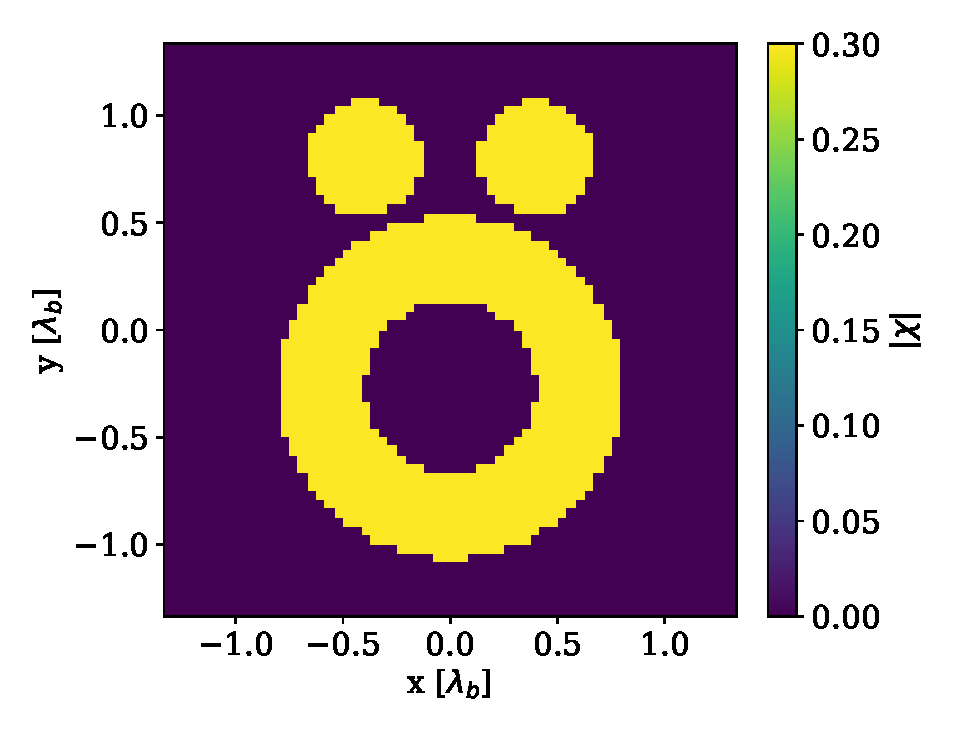
\includegraphics[width=.25\textwidth]{./figuras/casestudy/austria/groundtruth}\label{fig:results:casestudy:austria:reconstruction:groundtruth}}
				\subfloat[SAEA1]{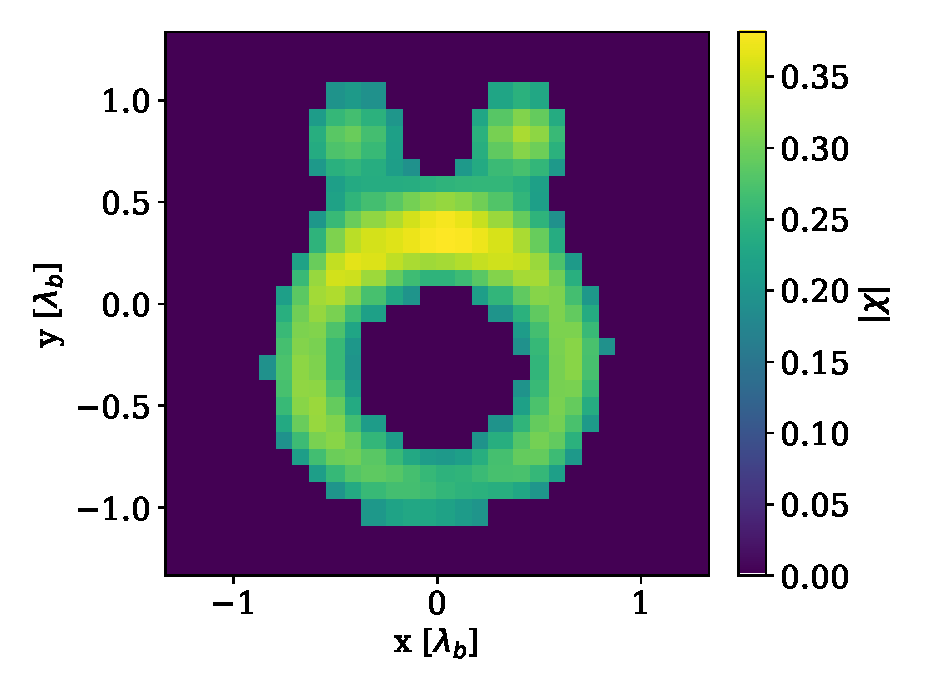
\includegraphics[width=.25\textwidth]{./figuras/casestudy/austria/reconstruction_saea1}\label{fig:results:casestudy:austria:reconstruction:saea1}}
				\subfloat[SAEA2]{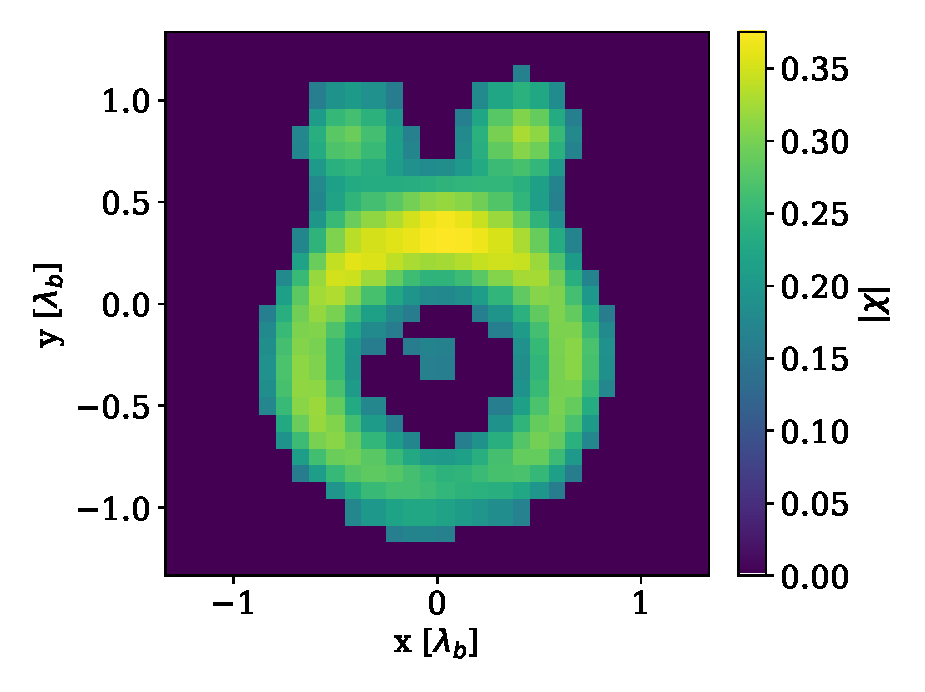
\includegraphics[width=.25\textwidth]{./figuras/casestudy/austria/reconstruction_saea2}\label{fig:results:casestudy:austria:reconstruction:saea2}}
				\subfloat[SAEA3]{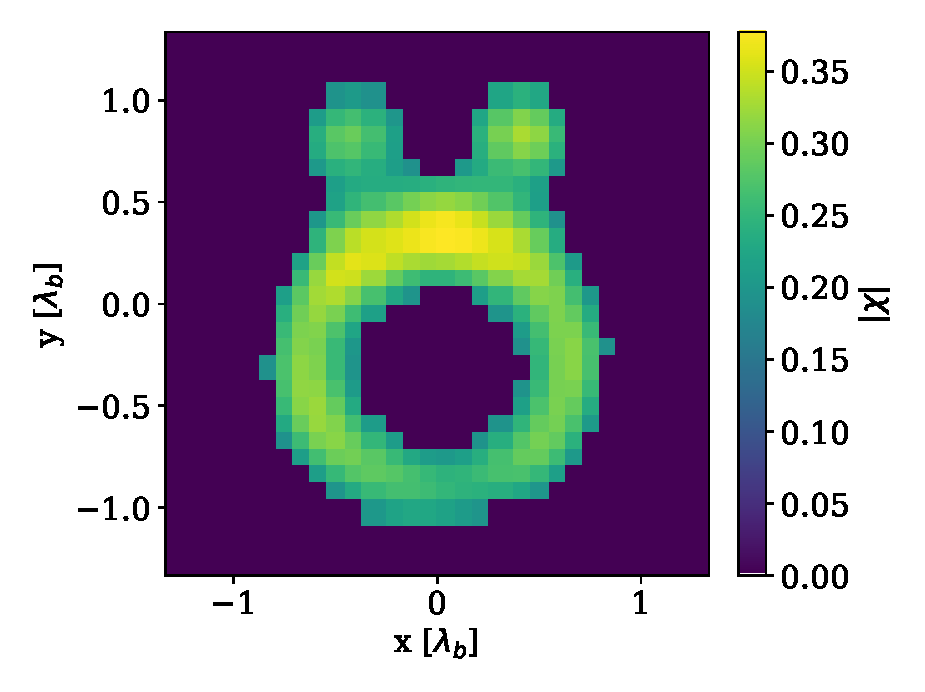
\includegraphics[width=.25\textwidth]{./figuras/casestudy/austria/reconstruction_saea3}\label{fig:results:casestudy:austria:reconstruction:saea3}} \\
				\subfloat[SADM1]{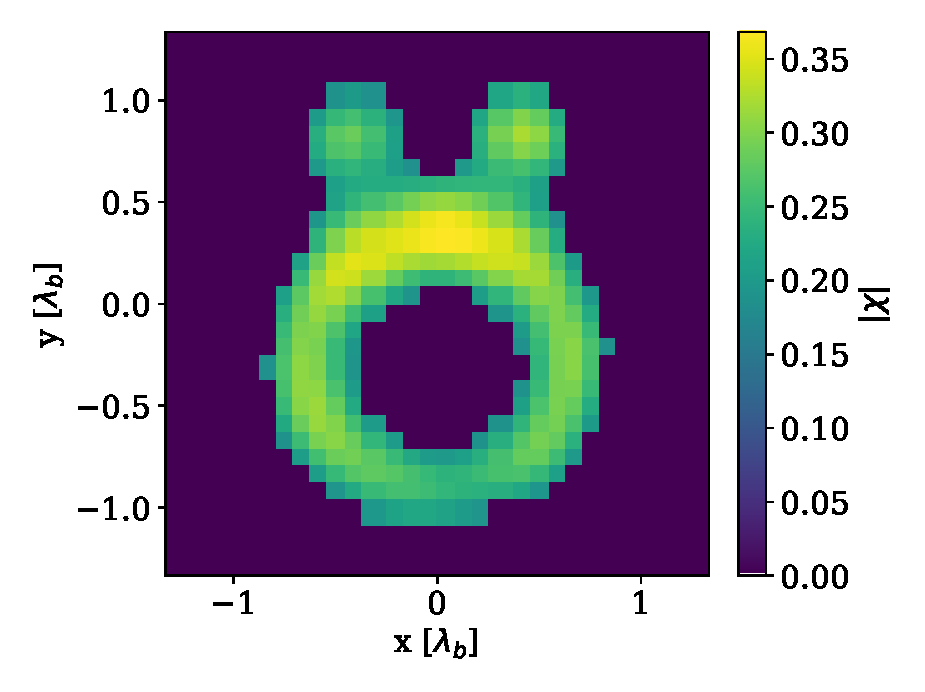
\includegraphics[width=.25\textwidth]{./figuras/casestudy/austria/reconstruction_sadm1}\label{fig:results:casestudy:austria:reconstruction:sadm1}}
				\subfloat[SADM2]{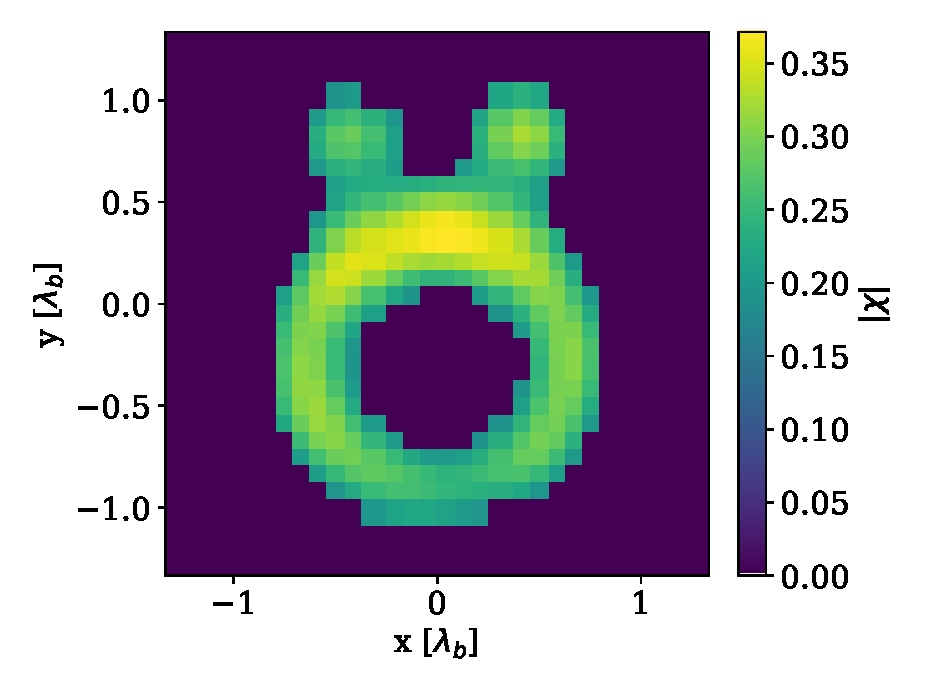
\includegraphics[width=.25\textwidth]{./figuras/casestudy/austria/reconstruction_sadm2}\label{fig:results:casestudy:austria:reconstruction:sadm2}}
				\subfloat[EA]{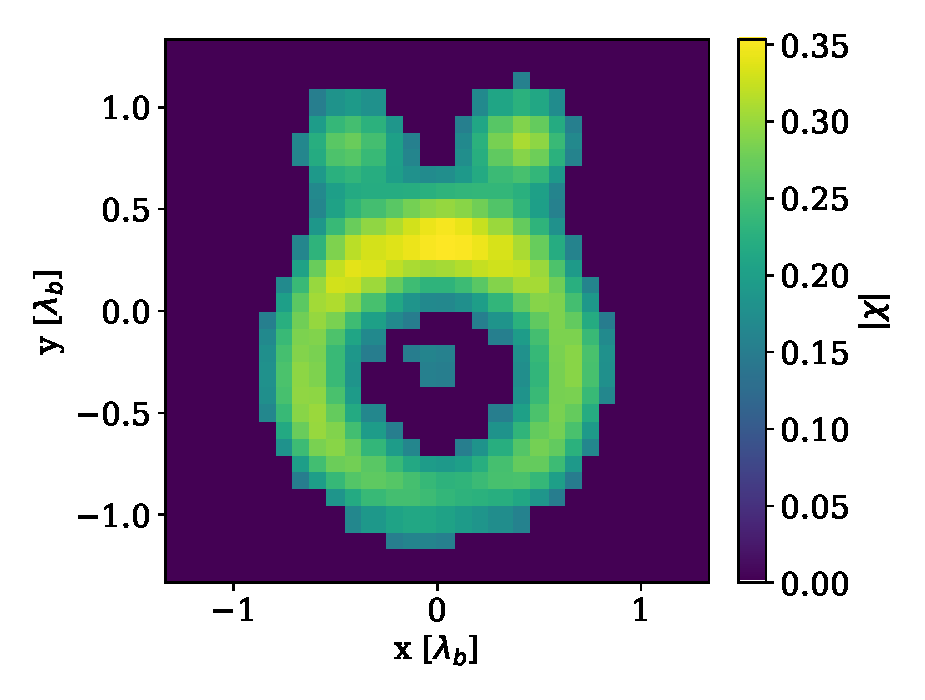
\includegraphics[width=.25\textwidth]{./figuras/casestudy/austria/reconstruction_ea}\label{fig:results:casestudy:austria:reconstruction:ea}}
				\subfloat[BIM]{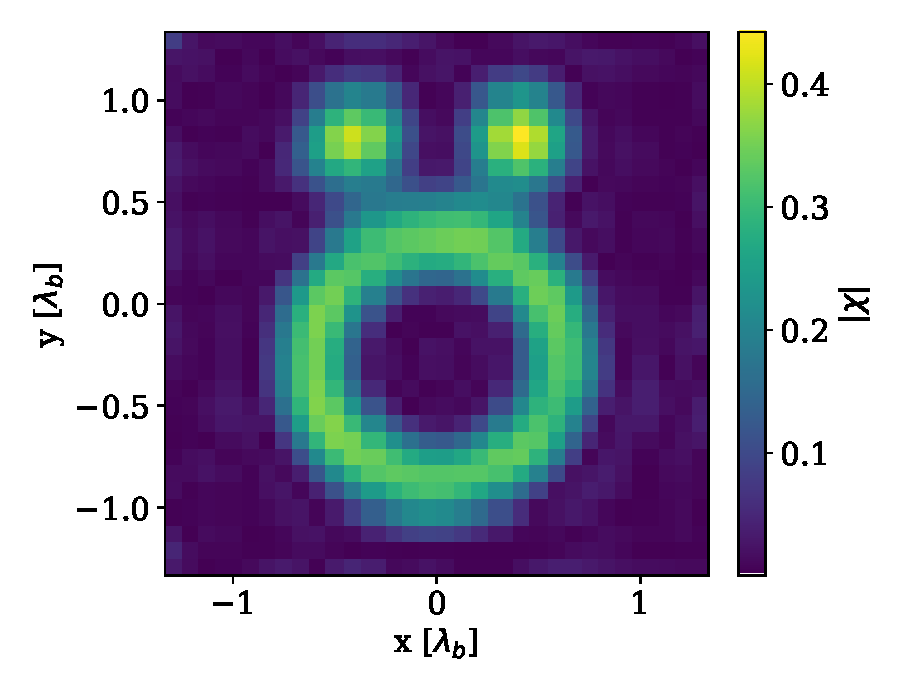
\includegraphics[width=.25\textwidth]{./figuras/casestudy/austria/reconstruction_bim}\label{fig:results:casestudy:austria:reconstruction:bim}} \\
				\subfloat[DBIM]{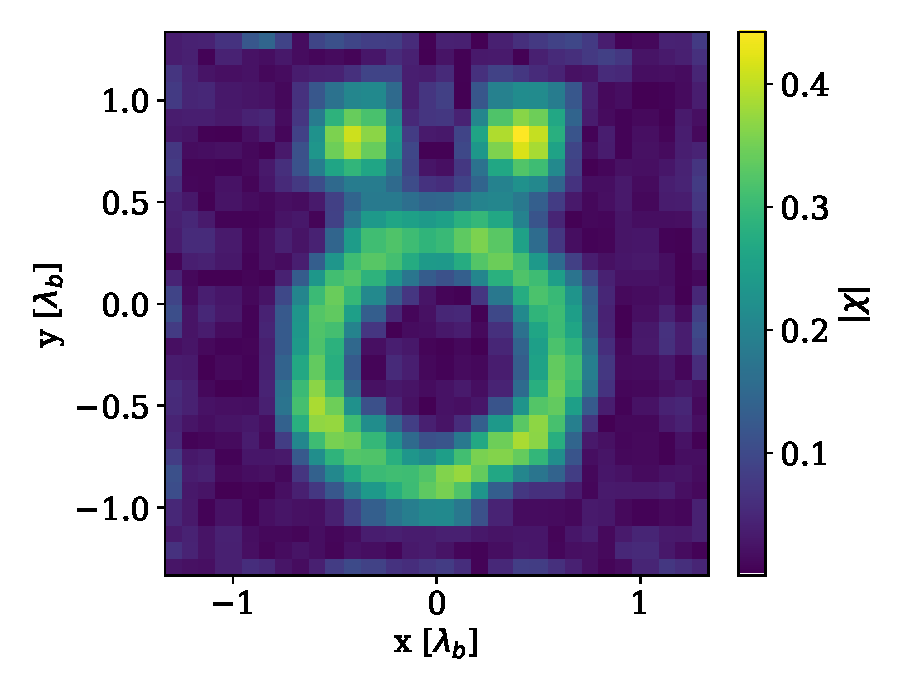
\includegraphics[width=.25\textwidth]{./figuras/casestudy/austria/reconstruction_dbim}\label{fig:results:casestudy:austria:reconstruction:dbim}}
				\subfloat[CGM]{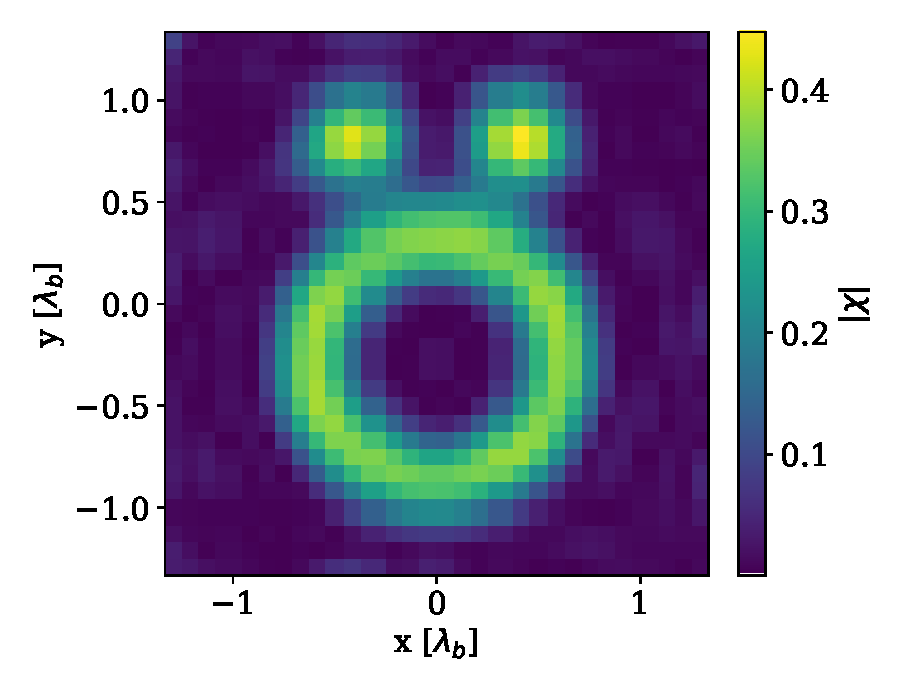
\includegraphics[width=.25\textwidth]{./figuras/casestudy/austria/reconstruction_cgm}\label{fig:results:casestudy:austria:reconstruction:cgm}}
				\subfloat[ECSI]{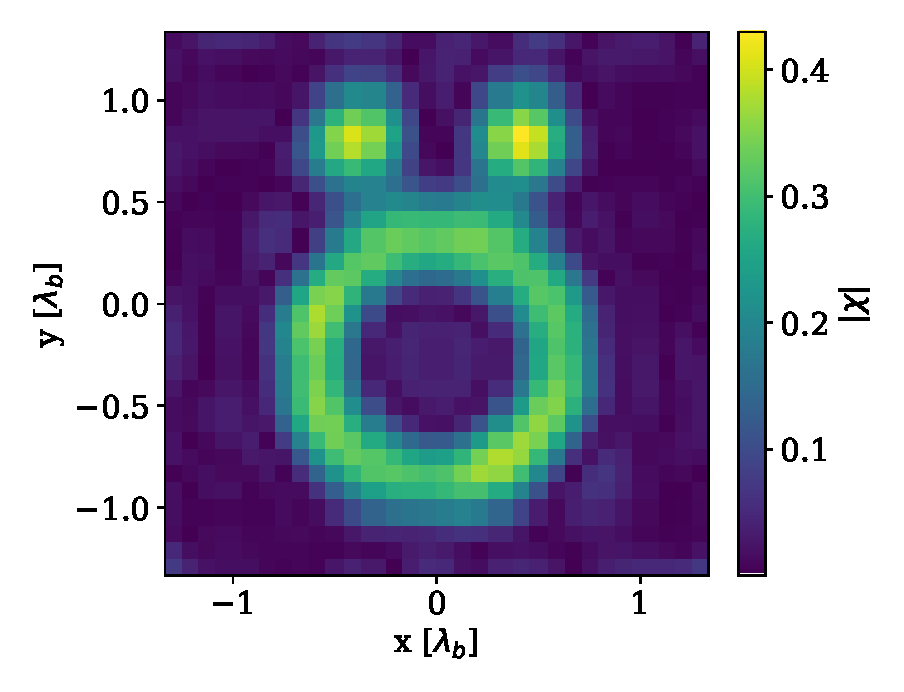
\includegraphics[width=.25\textwidth]{./figuras/casestudy/austria/reconstruction_ecsi}\label{fig:results:casestudy:austria:reconstruction:ecsi}}
				\subfloat[SOM]{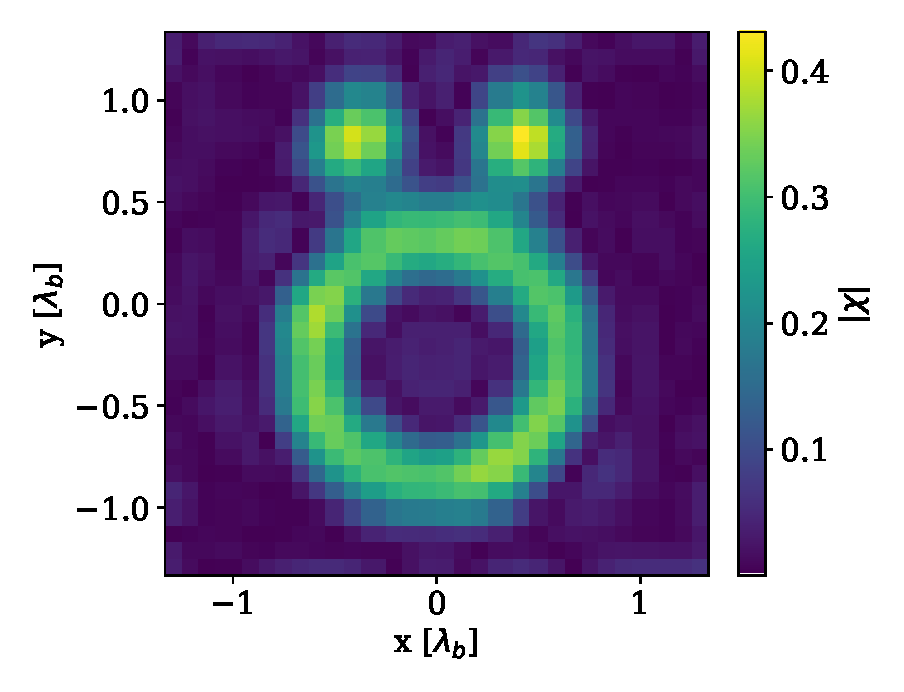
\includegraphics[width=.25\textwidth]{./figuras/casestudy/austria/reconstruction_som}\label{fig:results:casestudy:austria:reconstruction:som}} 
				\caption[Austria profile case study: Comparison of image reconstructions using surrogate model-assisted algorithms and deterministic methods.]{Comparison of image reconstructions using surrogate model-assisted algorithms and deterministic methods considering the Austria profile case study: (a) shows the ground-truth image; (b), (c), and (d) depict the best image recovered by SAEA1, SAEA2, and SAEA3, respectively, in 30 execution according to $\zeta_{\epsilon OE}$ indicator; (e), (f) and (g) show the best image recovered by SADM1, SADM2, and EA, respectively, in 30 execution according to $\zeta_{\epsilon OE}$ indicator; (g) shows the image recovered by BIM, and (h) shows the image recovered by DBIM; finally, (i), (k), and (l) show the image recovered by CGM, ECSI, and SOM, respectively.}
				\label{fig:results:casestudy:austria:reconstruction}
			\end{figure}
		
			% 1. A Fig. \ref{fig:results:casestudy:austria:reconstruction} mostra a melhor das reconstruções dentre as 30 execuções de cada algoritmo estocástico, de acordo com o indicador $\zeta_{\epsilon OE}$ (Figs. \ref{fig:results:casestudy:austria:reconstruction:saea1}-\ref{fig:results:casestudy:austria:reconstruction:ea}).
			% 2. A figura também mostra as reconstruções dos algoritmos determinísticos (Figs. \ref{fig:results:casestudy:austria:reconstruction:bim}-\ref{fig:results:casestudy:austria:reconstruction:som}).
			% 3. Todos os algoritmos fizeram uma ligeira superestimativa do contraste, conforme indica o valor máximo de contraste em cada figura. Essa suppdferestimativa tende a ser ligeiramente menor nos algoritmos baseados na proposta de transformação do problema. Este efeito tende a ser uma compensação pela subestimativa nas bordas do espalhador.
			% 4. Eles mostram também uma certa dificuldade em detectar bem a separação entre o anel e os dois círculos. Essa dificuldade está relacionada com a proximidade entre esses objetos.
			% 4. As melhores imagens reconstruídas pelo SAEA2 e pelo EA mostram um pequeno objeto fantasma dentro do anel da imagem. Isso é um problema do ajuste do valor do limiar. Como o indicador $\zeta_{\epsilon OE}$ só leva em consideração a estimativa dentro da região original do espalhador, então erros na região de fundo original do problema não são levados em conta.
			% 5. Como era de se esperar, os algoritmos baseados na transformação do problema em um de otimização bidimensional mostram uma região de fundo mais limpa. Isto é devido ao operador de limiarização. O BIM (Fig. \ref{fig:results:casestudy:austria:convergence:bim}) também apresenta uma região de fundo um pouco mais limpa que o DBIM (Fig. \ref{fig:results:casestudy:austria:convergence:dbim}) e isso está associado à dificuldade do DBIM com níveis de ruído significativos.
			
			In the results of the case study, Fig. \ref{fig:results:casestudy:austria:reconstruction} displays the best of the reconstructions among the 30 runs of each stochastic algorithm, based on indicator $\zeta_{\epsilon OE}$ (Figs. \ref{fig:results:casestudy:austria:reconstruction:saea1}-\ref{fig:results:casestudy:austria:reconstruction:ea}), and also includes the reconstructions of the deterministic algorithms (Figs. \ref{fig:results:casestudy:austria:reconstruction:bim}-\ref{fig:results:casestudy:austria:reconstruction:som}). The figures show that all algorithms overestimated the contrast slightly, which can be seen in the maximum contrast value in each figure. However, algorithms based on the problem transformation proposal tended to have slightly lower overestimation, which compensates for underestimation at the edges of the scatterer. The reconstructions also had some difficulty in detecting the separation between the ring and the two circles, which was related to the proximity between these objects. Additionally, the best SAEA2 and EA reconstructed images showed a small ghost object inside the image ring due to a threshold value adjustment issue. As the $\zeta_{\epsilon OE}$ indicator only takes into account the estimate within the original region of the scatterer, then errors in the original background region of the problem do not influence the indicator. Furthermore, algorithms based on transforming the problem into a two-dimensional optimization problem showed a cleaner background region, which was attributed to the thresholding operator. BIM (Fig. \ref{fig:results:casestudy:austria:convergence:bim}) presented a slightly cleaner background region than DBIM (Fig. \ref{fig:results:casestudy:austria:convergence:dbim}), which was associated with the difficulty of DBIM in dealing with significant noise levels.
		
			\begin{figure}[!h]
				\centering
				\subfloat[SAEA1]{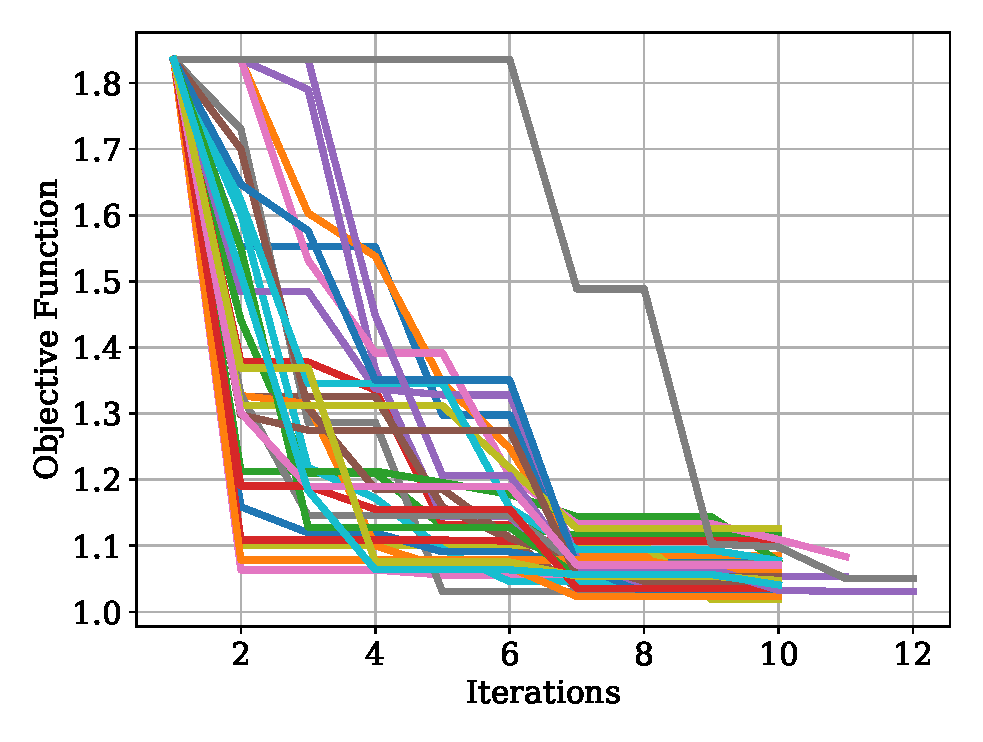
\includegraphics[width=.25\textwidth]{./figuras/casestudy/austria/convergence_saea1}\label{fig:results:casestudy:austria:convergence:saea1}}
				\subfloat[SAEA2]{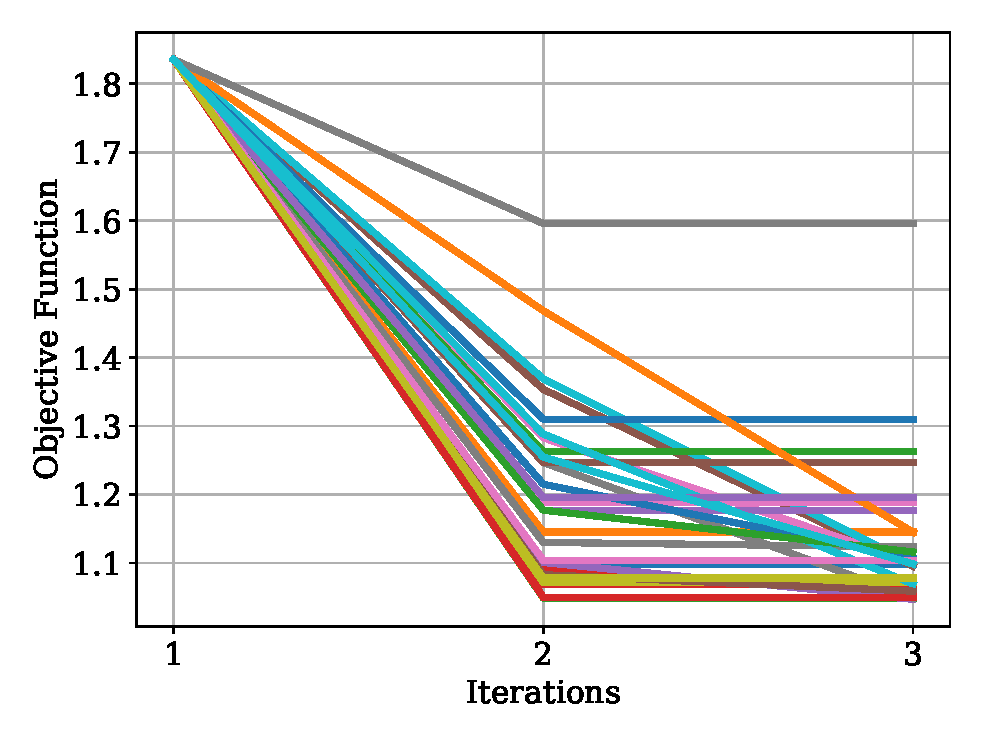
\includegraphics[width=.25\textwidth]{./figuras/casestudy/austria/convergence_saea2}\label{fig:results:casestudy:austria:convergence:saea2}}
				\subfloat[SAEA3]{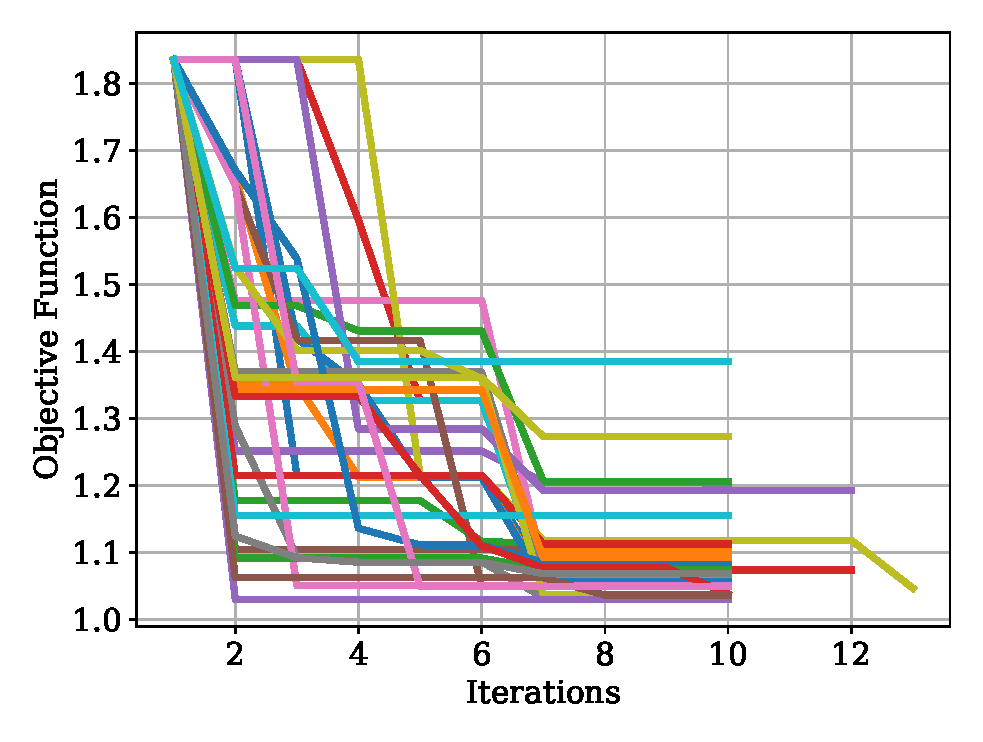
\includegraphics[width=.25\textwidth]{./figuras/casestudy/austria/convergence_saea3}\label{fig:results:casestudy:austria:convergence:saea3}}
				\subfloat[SADM1]{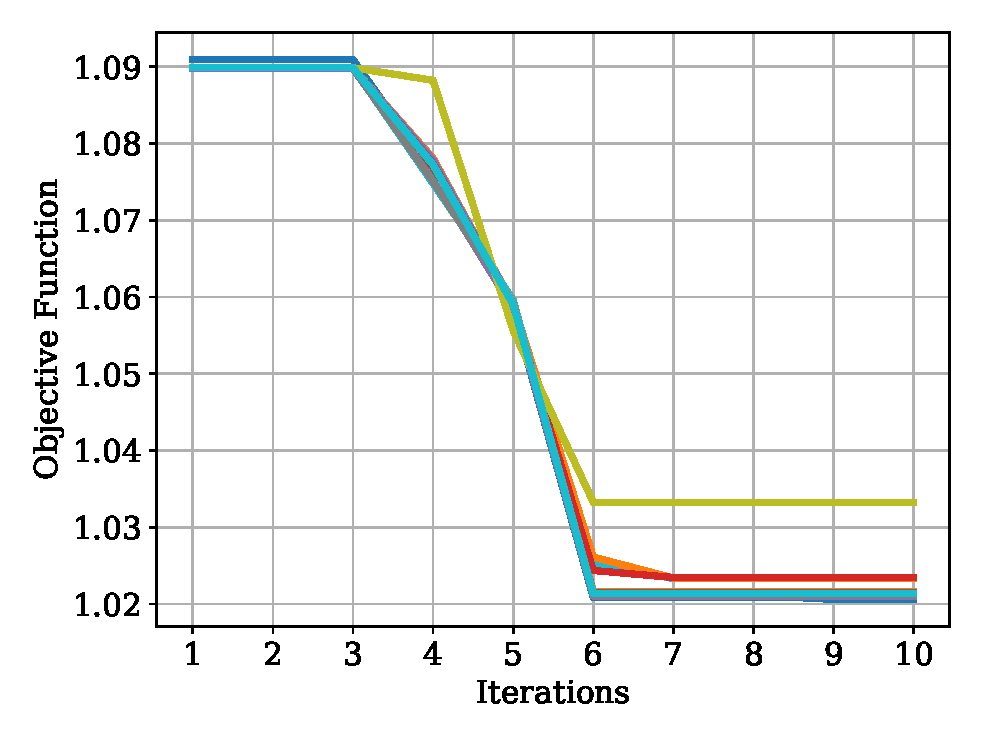
\includegraphics[width=.25\textwidth]{./figuras/casestudy/austria/convergence_sadm1}\label{fig:results:casestudy:austria:convergence:sadm1}} \\
				\subfloat[SADM2]{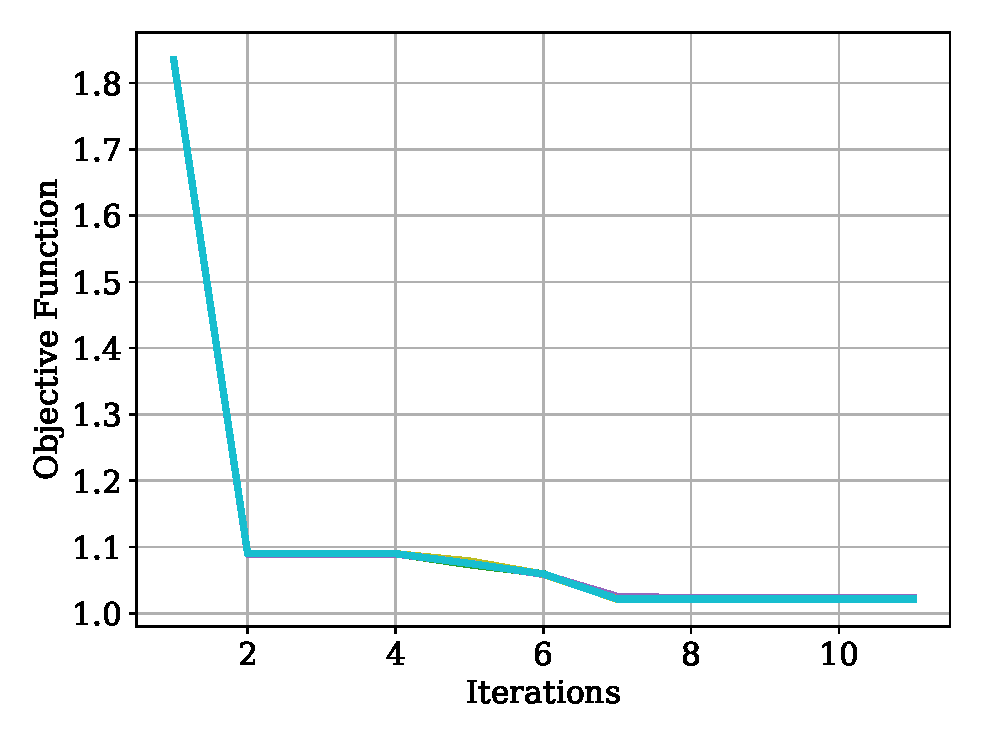
\includegraphics[width=.25\textwidth]{./figuras/casestudy/austria/convergence_sadm2}\label{fig:results:casestudy:austria:convergence:sadm2}}
				\subfloat[EA]{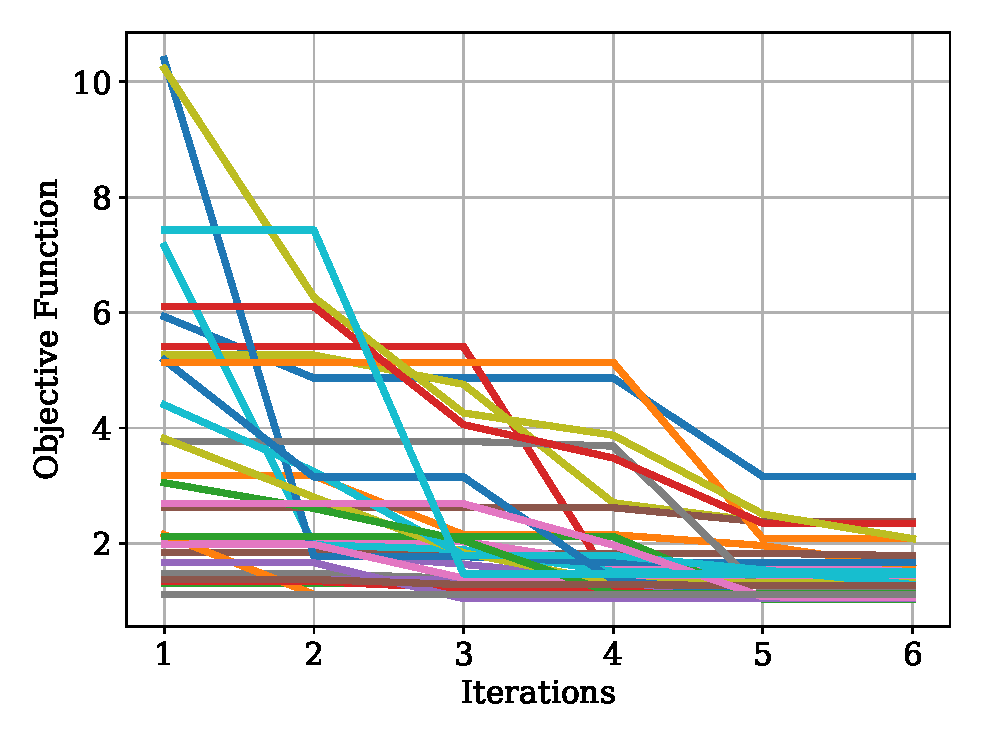
\includegraphics[width=.25\textwidth]{./figuras/casestudy/austria/convergence_ea}\label{fig:results:casestudy:austria:convergence:ea}}
				\subfloat[BIM]{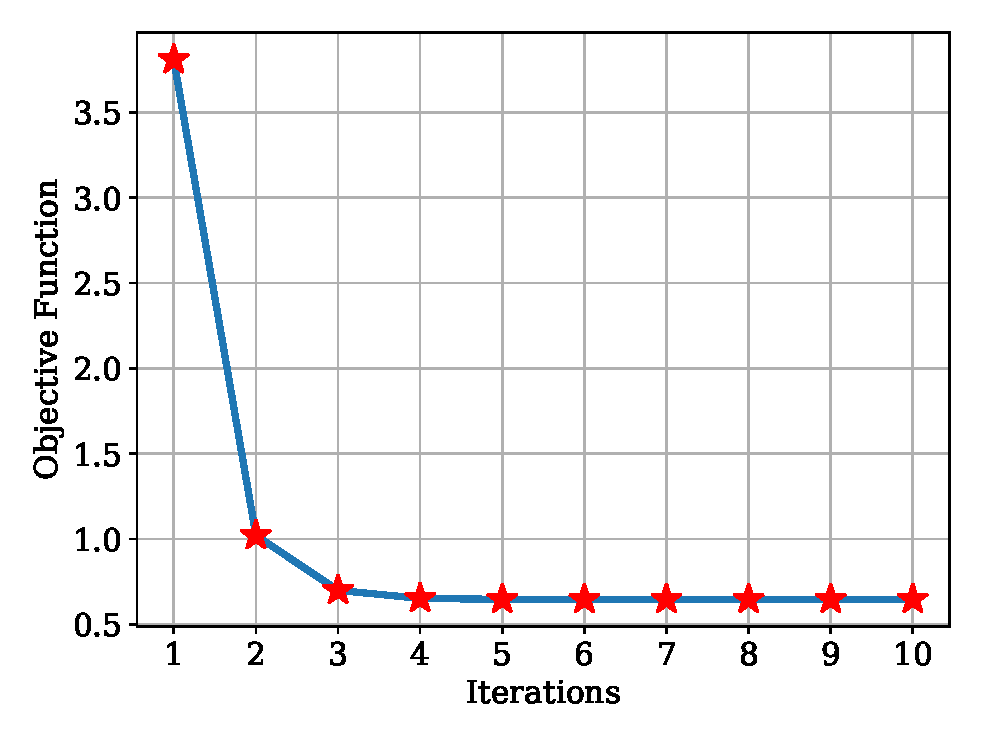
\includegraphics[width=.25\textwidth]{./figuras/casestudy/austria/convergence_bim}\label{fig:results:casestudy:austria:convergence:bim}}
				\subfloat[DBIM]{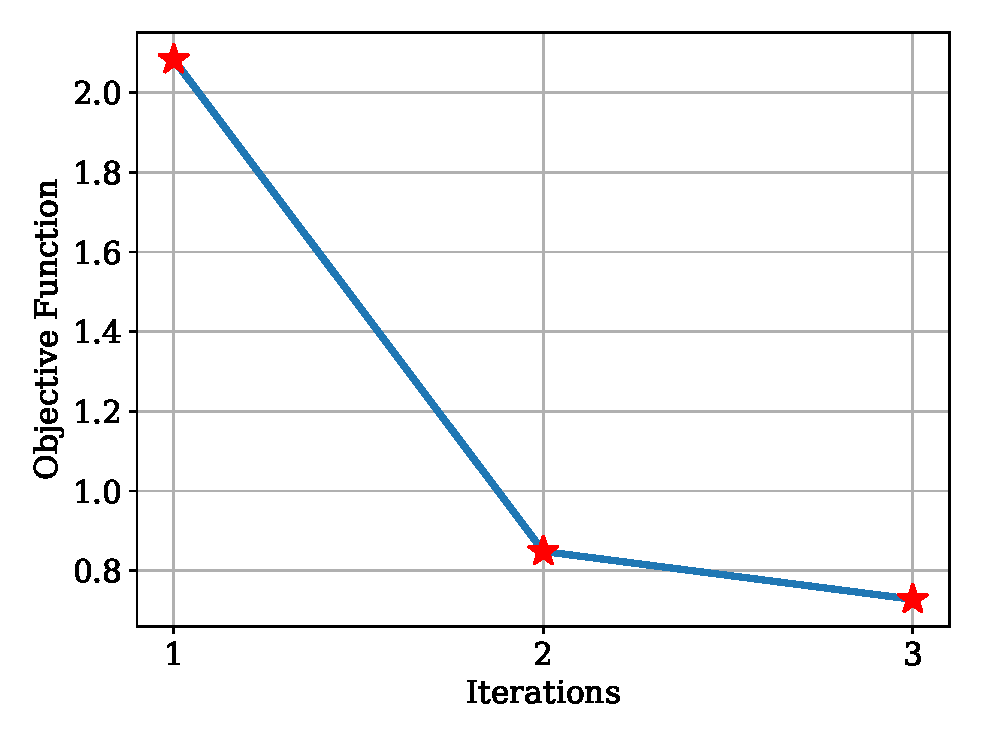
\includegraphics[width=.25\textwidth]{./figuras/casestudy/austria/convergence_dbim}\label{fig:results:casestudy:austria:convergence:dbim}} \\
				\subfloat[CGM]{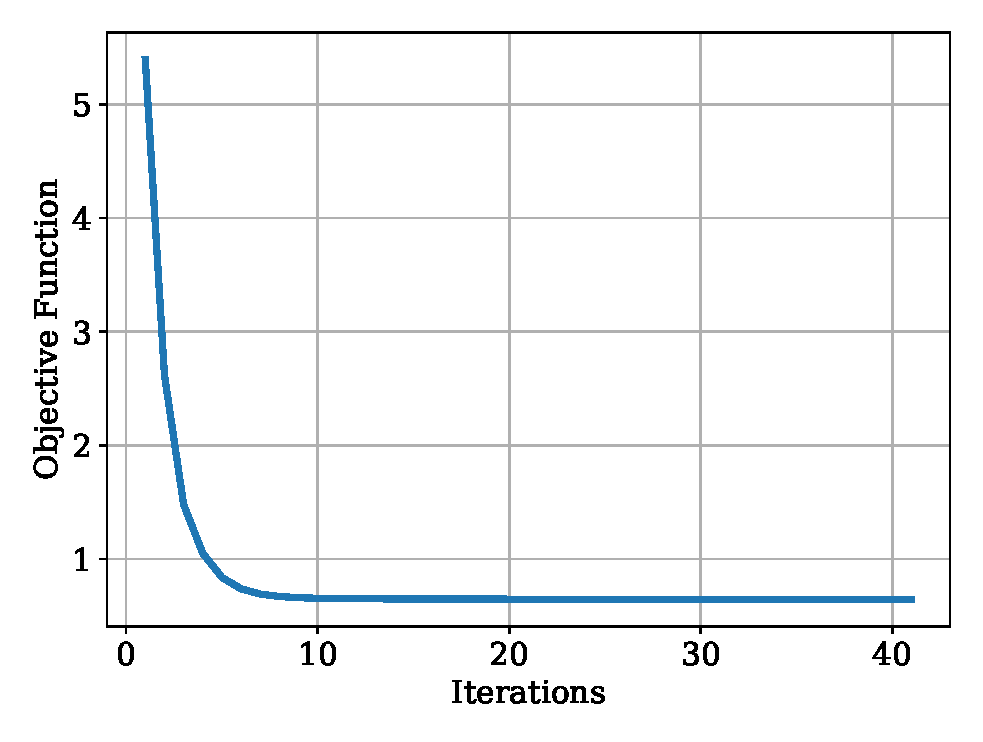
\includegraphics[width=.25\textwidth]{./figuras/casestudy/austria/convergence_cgm}\label{fig:results:casestudy:austria:convergence:cgm}}
				\subfloat[ECSI]{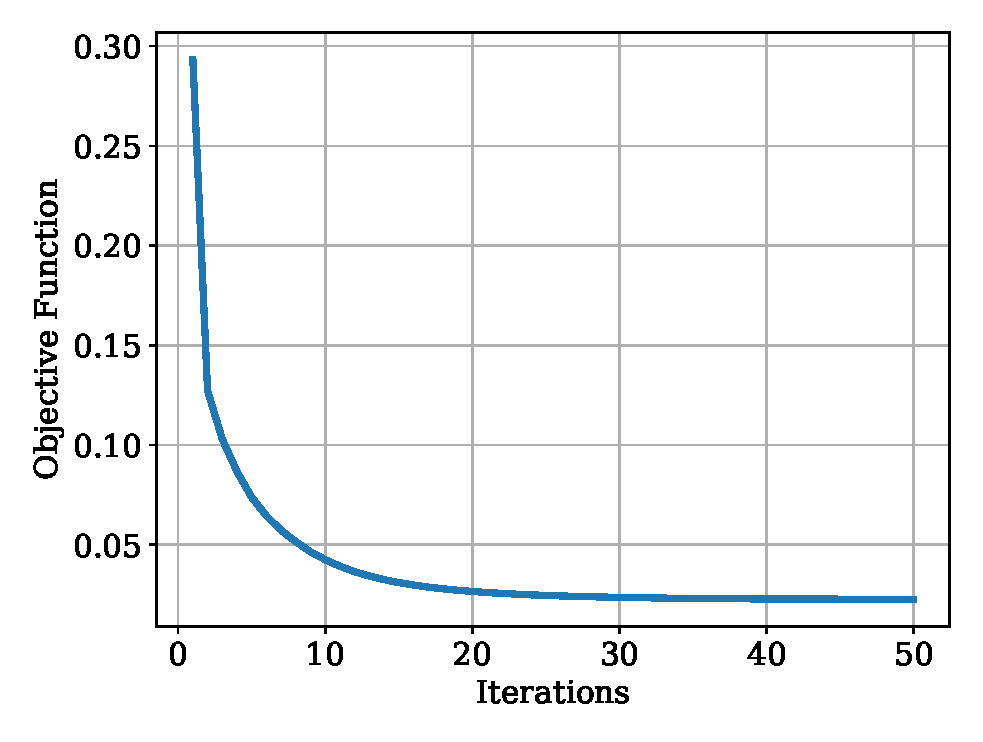
\includegraphics[width=.25\textwidth]{./figuras/casestudy/austria/convergence_ecsi}\label{fig:results:casestudy:austria:convergence:ecsi}}
				\subfloat[SOM]{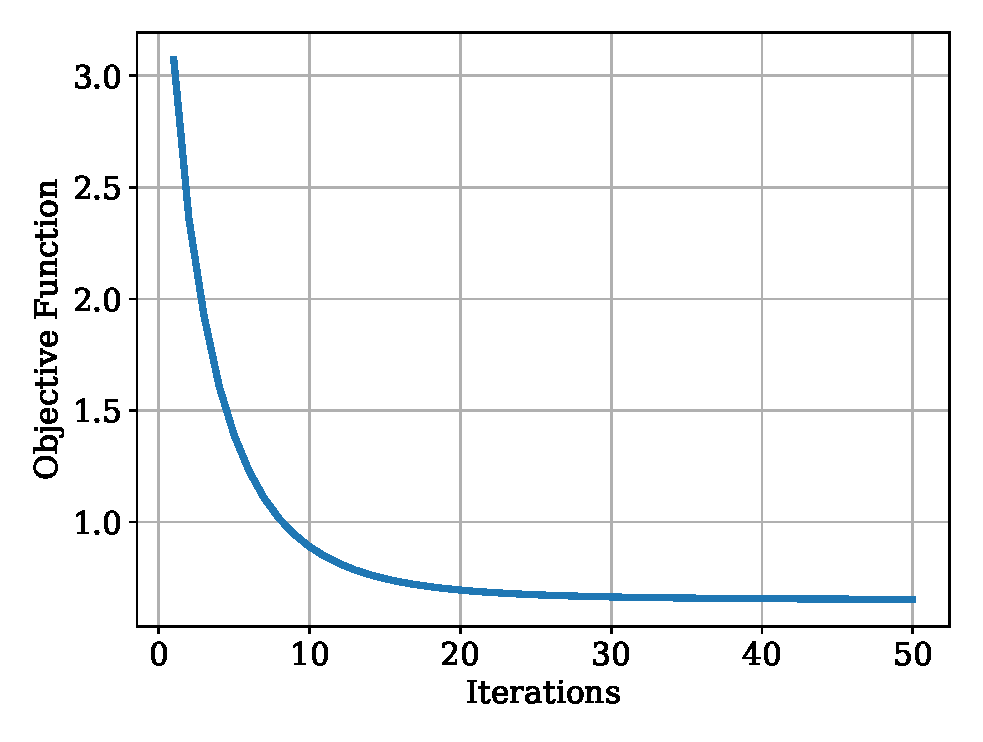
\includegraphics[width=.25\textwidth]{./figuras/casestudy/austria/convergence_som}\label{fig:results:casestudy:austria:convergence:som}} 
				\caption[Convergence of the objective function for the Austria profile case obtained by the stochastic and deterministic algorithms.]{Convergence of the objective function for the Austria profile case obtained by the stochastic and deterministic algorithms. (a) to (k) show the curves obtained by SAEA1, SAEA2, SAEA3, SADM1, SADM2, EA, BIM, DBIM, CGM, ECSI, and SOM algorithms, respectively. The x-axis represents the number of iterations, and the y-axis represents the value of the objective function of the correspondent algorithm.}
				\label{fig:results:casestudy:austria:convergence}
			\end{figure}
		
			% 1. A Fig. \ref{fig:results:casestudy:austria:convergence} mostra a curva de convergência da função-objetivo para cada algoritmo.
			% 2. Como cada algoritmo determinístico tem sua própria função-objetivo que pauta a sua estrutura, o eixo y só pode ser comparado entre os algoritmos baseados na otimização bidimensional (Figs. \ref{fig:results:casestudy:austria:convergence:saea1}-\ref{fig:results:casestudy:austria:convergence:ea}).
			% 3. O SAEA3 teve somente 3 gerações. O número baixo é explicado pelo fato de que cada iteração o número de avaliações da função-objetivo verdadeira é igual ao tamanho da população. Isto é diferente do SAEA1 e do SAEA3 que gastam somente uma avaliação por geração.
			% 4. Mesmo com poucas gerações, o SAEA2 ainda assim termina as execuções com valores próximos dos alcançados pelo SAEA1 e pelo SAEA3. Isso tem a ver com o bom mapeamento do espaço de busca feito pela população inicial.
			% 5. Os valores finais alcançados pelo SAEA1 nas 30 execuções foram mais semelhantes que os do SAEA3. Isto pode sugerir que a convergência do SAEA1 é melhor.
			% 6. Algumas execuções do SADM1 não convergiram para o mesmo local que a maioria. Isto pode ser um efeito do processo estocástico de busca por solução inicial. O mesmo não acontece para o SADM2. Todas as execuções desse algoritmo convergiram igualmente, indicando um comportamento determinístico.
			% 7. O EA tem mais gerações que o SAEA2 porque o EA não tem a necessidade de gerar uma amostra inicial de soluções. No entanto, o número maior de gerações não contribuiu para alcançar mais rapidamente a região perto do mínimo. Isso é mais factível para o SAEA2 por causa da estratégia de amostragem de soluções.
			
			The convergence curve for each algorithm is shown in Fig. \ref{fig:results:casestudy:austria:convergence}. The y-axis can only be compared between algorithms based on two-dimensional optimization (Figs. \ref{fig:results:casestudy:austria:convergence:saea1}-\ref{fig:results:casestudy:austria:convergence:ea}), as each deterministic algorithm has its own objective function that guides its structure. SAEA2 had a few generations but still achieved values close to those achieved by SAEA1 and SAEA3, thanks to the good mapping of the search space done by the initial population. The final values reached by SAEA1 in the 30 runs were more similar than those by SAEA3, which may suggest that SAEA1 convergence is better.
			
			Some SADM1 runs did not converge to the same location as most, which may be an effect of the stochastic search process for the initial solution. The same does not happen for SADM2, as all executions of this algorithm converged equally, indicating a deterministic behavior. The EA has more generations than the SAEA2, but the greater number of generations did not contribute to reaching the region closer to the minimum more quickly. This is straightforward for SAEA2 because of the solution sampling strategy.			
		
			\begin{figure}
				\centering
				\subfloat[]{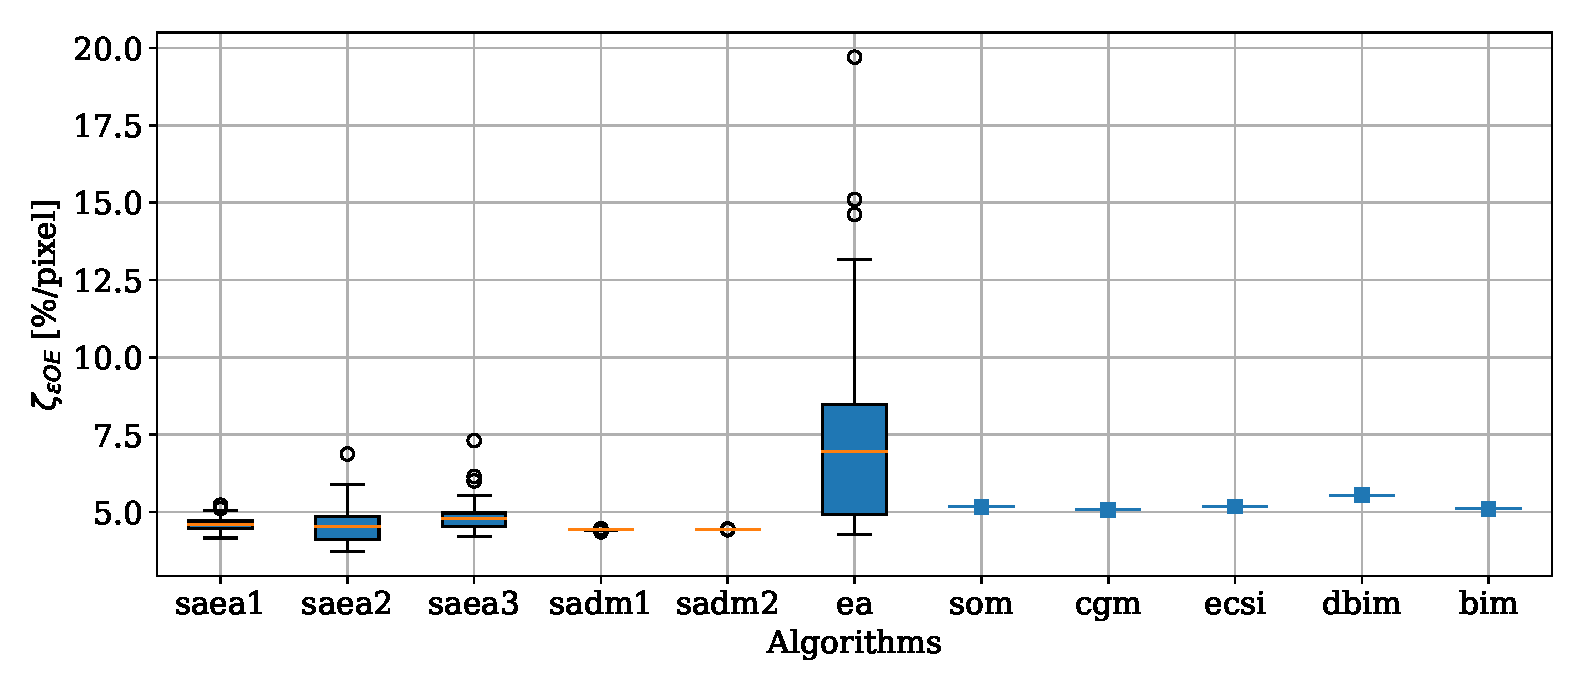
\includegraphics[width=.9\textwidth]{./figuras/casestudy/austria/boxplot_zeta_eoe_ea}\label{fig:results:casestudy:austria:boxplot:zeta_eoe:withea}} \\
				\subfloat[]{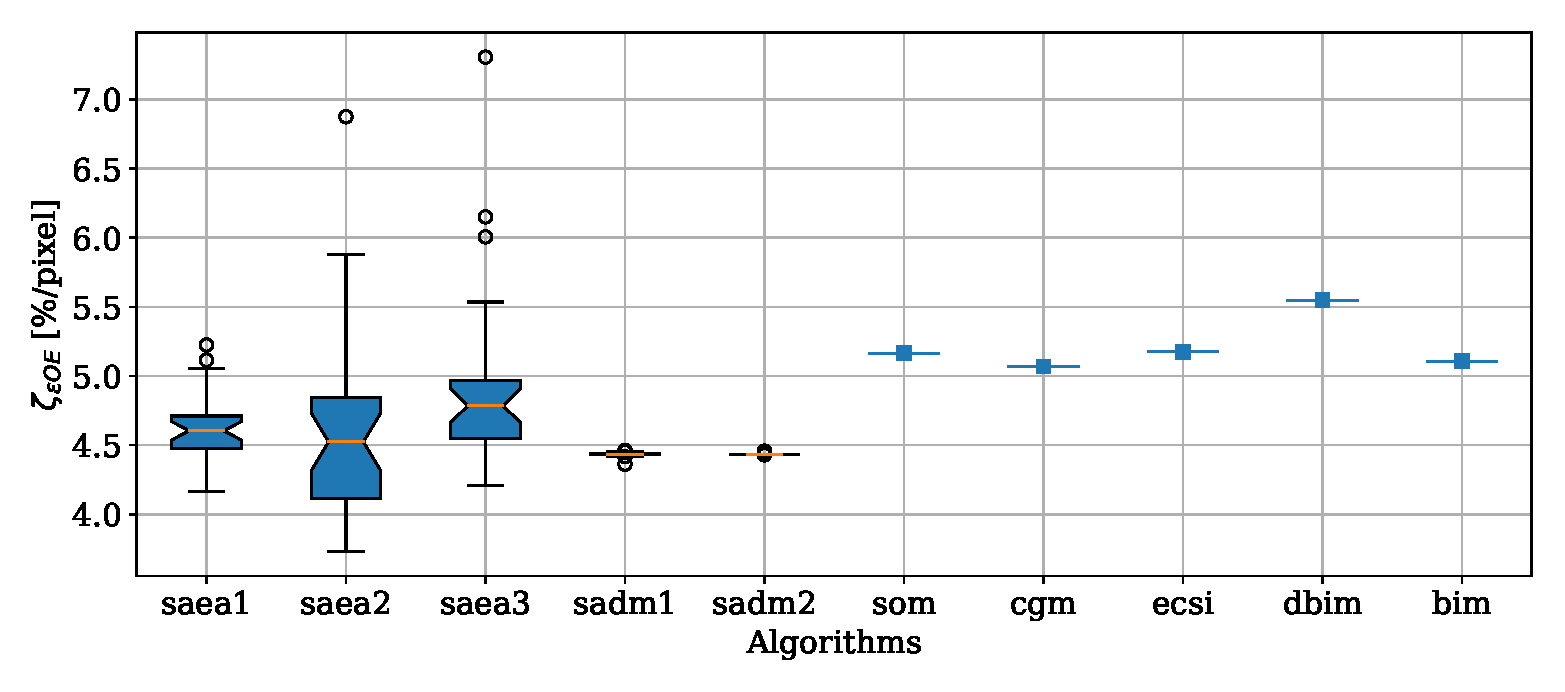
\includegraphics[width=.9\textwidth]{./figuras/casestudy/austria/boxplot_zeta_eoe}\label{fig:results:casestudy:austria:boxplot:zeta_eoe:noea}}
				\caption[Performance of $\zeta_{\epsilon OE}$ indicator for various algorithms in the Austria profile.]{Performance of $\zeta_{\epsilon OE}$ indicator for various algorithms in the Austria profile. (a) Boxplots show quartiles of 30 executions for stochastic algorithms, and the solid line represents the deterministic algorithms. (b) Exclusion of the EA algorithm for better visualization of differences among algorithms.}
				\label{fig:results:casestudy:austria:boxplot:zeta_eoe}
			\end{figure}
		
			% 1. A Fig. \ref{fig:results:casestudy:austria:boxplot:zeta_eoe:withea} mostra os quartis do indicador $\zeta_{\epsilon OE}$ para os algoritmos nos quais foram executadas 30 execuções e o valor alcançados pelos determinísticos.
			% 2. Os quartis do EA se destacam negativamente. Tal dificuldade por encontrar uma boa estimativa final do contraste do espalhador tem a ver com a necessidade que o algoritmo tem de mais gerações para poder convergir para mais perto do ótimo, como nos outros algoritmos assistidos por modelos substitutos.
			% 3. Removendo os dados do EA (Fig. \ref{fig:results:casestudy:austria:boxplot:zeta_eoe:noea}), é possível visualizar melhor as diferenças entre os algoritmos assistidos por modelos substitutos e os determinísticos. A mediana dos algoritmos assistidos por modelos substitutos ficaram abaixo de todos os determinísticos. Em especial, todas as execuções do SADM1 e do SADM2 ficaram abaixo do erro de estimativa de contraste dos determinísticos. No entanto, houveram execuções dos SAEA's que terminaram com um erro menor.
			% 4. Todas as execuções do SADM2 terminaram com o mesmo erro, uma vez que todas as execuções convergiram de igual modo (conforme visto na Fig. \ref{fig:results:casestudy:austria:convergence:sadm2}). Embora a convergência do SADM1 não tenha sido tão igual entre as execuções, eles alcançaram o mesmo erro. Isso indica que a solução final de cada execução foi muito próxima.
			% 5. O erro da estimativa de contraste dos algoritmos assistidos por modelos substitutos tem a ver com o local da superfície de otimização no qual eles terminam.
			% 6. De uma maneira geral, o resultado indica que a abordagem de transformação do problema pode ser bem sucedida de forma a fazer uma estimativa de contraste melhor na mediana dos casos, comparando com as abordagens tradicionais. No entanto, em cenários de espalhadores fracos, essa diferença não é tão significativa conforme mostra os gráficos (até 1.5 [\%/pixel]).
			
			Fig. \ref{fig:results:casestudy:austria:boxplot:zeta_eoe:withea} shows the $\zeta_{\epsilon OE}$ indicator quartiles for the algorithms in which 30 executions were performed and the value reached by the deterministic ones. The EA quartiles stand out negatively, as the algorithm has difficulty finding a good final estimate of the scatterer contrast. This is attributed to the algorithm's need for more generations to converge closer to the optimum, as in other algorithms assisted by surrogate models.
			
			By removing the EA data (Fig. \ref{fig:results:casestudy:austria:boxplot:zeta_eoe:noea}), it is possible to better visualize the differences between the algorithms assisted by surrogate models and the deterministic ones. The median of algorithms assisted by surrogate models was below all deterministic ones. In particular, all SADM1 and SADM2 runs were below the deterministic contrast estimation error. However, there have been executions of SAEA's that ended with a minor error. All runs of SADM2 ended with the same error since all runs converged equally (as seen in Fig. \ref{fig:results:casestudy:austria:convergence:sadm2}). Although SADM1 convergence was not as equal between runs, they achieved the same error, indicating that the final solution for each run was very close. The Kruskal-Wallis H-Test confirmed difference among SAEA1, SAEA2, and SAEA3 (p-value $=0.0219$), and all-to-all comparison by Mann-Whitney U test confirmed that SAEA1 and SAEA2 overperformed SAEA3 (p-values 0.0199 and 0.0191, respectively). The Multiple Mann-Whitney U test did not detected difference between SADM1 and SADM2 (p-value $=0.0505$).
			
			The contrast estimation error of surrogate model-assisted algorithms has to do with where on the optimization surface they end up. In general, the result indicates that the problem transformation approach can be successful in making a better contrast estimate in the median of cases compared to the traditional approaches. However, in weak scattering scenarios, this difference is not as significant as the graphs show (up to 1.5 [\%/pixel]).
		
			\begin{figure}
				\centering
				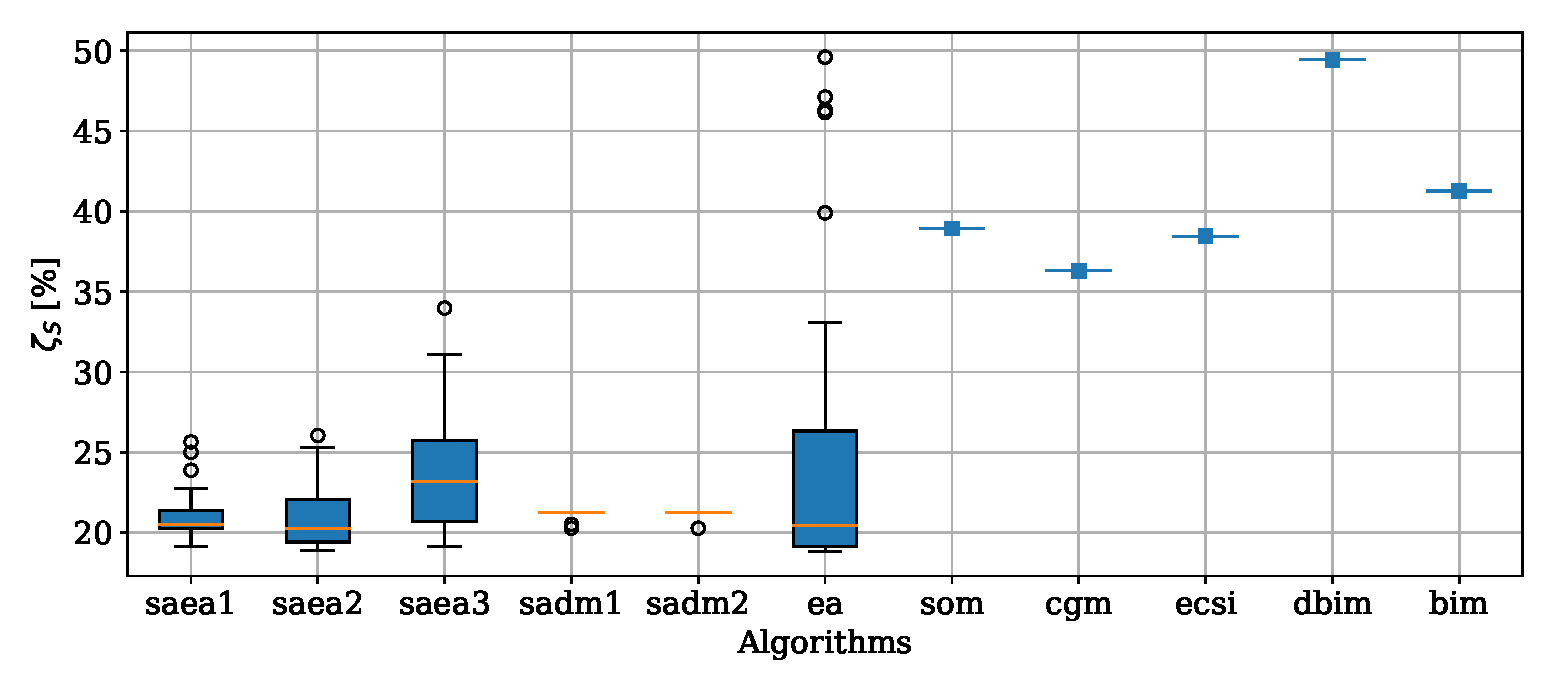
\includegraphics[width=.9\textwidth]{./figuras/casestudy/austria/boxplot_zeta_s}
				\caption[Performance of shape error estimation quantified by the $\zeta_S$ indicator obtained by the set of algorithms considering the Austria profile.]{Performance of shape error estimation quantified by the $\zeta_S$ indicator obtained by the set of algorithms considering the Austria profile. The boxes represent the quartiles of the 30 executions of the stochastic algorithms, while the other points indicate the obtained values by the deterministic ones. The shape error is calculated based on the ground-truth image and the reconstructed image obtained by each algorithm.}
				\label{fig:results:casestudy:austria:boxplot:zeta_s}
			\end{figure}
		
			% 1. Em relação ao erro de recuperação de forma $\zeta_S$ (Fig. \ref{fig:results:casestudy:austria:boxplot:zeta_s}), a diferença de desempenho é mais significativa entre os algoritmos determinísticos e aqueles baseados na transformação do problema. A diferença pode ser de até 20\%, aproximadamente, da área do espalhador original.
			% 2. O sucesso da abordagem de transformação proposta nos resultados de recuperação de forma está associado tanto à qualidade dos métodos qualitativos em fazer essa estimativa quanto na eficiência da operação de limiarização intrínseca à formulação.
			
			The performance of different algorithms for shape recovery error ($\zeta_S$) is shown in Fig. \ref{fig:results:casestudy:austria:boxplot:zeta_s}. The difference in performance between deterministic algorithms and those based on the transformation of the problem is more significant, up to approximately 20\% of the area of the original scatterer. The success of the proposed transformation approach in shape recovery results is associated with the quality of the qualitative methods used and the efficiency of the thresholding operation intrinsic to the formulation. The Kruskal-Wallis H-Test confirmed difference among SAEA1, SAEA2, and SAEA3 (p-value $<0.0002$), and all-to-all comparison by Multiple Mann-Whitney U test confirmed that SAEA1 and SAEA2 overperformed SAEA3 (p-values $<0.001$ for both cases). The Mann-Whitney U test detected difference suggesting that SADM1 outperform SADM2 (p-value $=0.013$).
		
			\begin{figure}
				\centering
				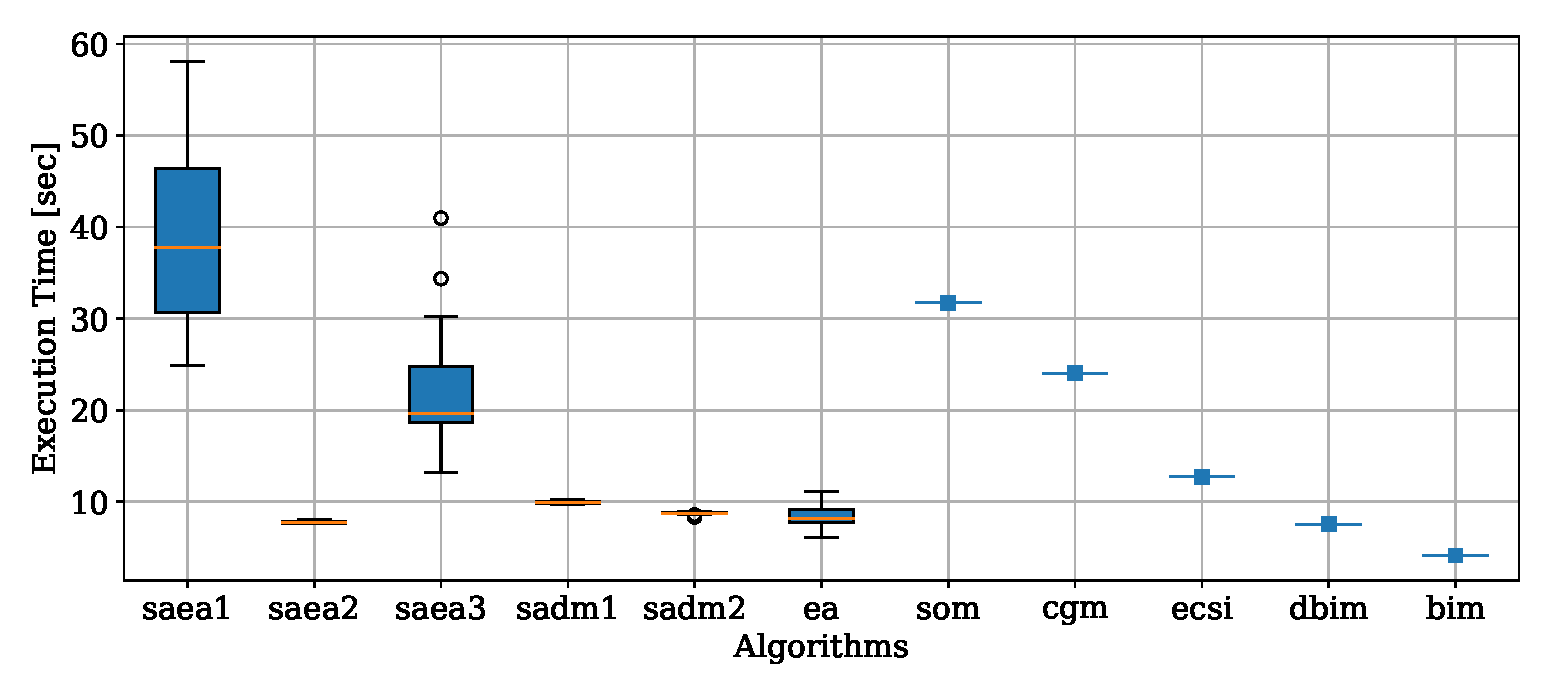
\includegraphics[width=.9\textwidth]{./figuras/casestudy/austria/boxplot_time}
				\caption[Box plot showing the execution time distribution of the set of algorithms considered for the Austria profile case.]{Box plot showing the execution time distribution of the set of algorithms considered for the Austria profile case. The boxes represent the quartiles of the 30 executions of the stochastic algorithms, and the whiskers represent the minimum and maximum values. The deterministic algorithms are represented by individual points. The execution time results are presented in seconds.}
				\label{fig:results:casestudy:austria:boxplot:time}
			\end{figure}
		
			% 1. A Fig. \ref{fig:results:casestudy:austria:boxplot:time} mostra o tempo de execução dos algoritmos.
			% 2. A mediana do SAEA1 foi a mais alta. Levando em conta somente as formulações do SAEA's, o SAEA2 foi o mais rápido, mesmo tendo o mesmo número de avaliações. Este resultado sugere o impacto de operações dentro do processo iterativo desses algoritmos, como o processo de busca local e o número de chamadas de treinamento do modelo que são menos acionados no SAEA2 para o mesmo número de avaliações.
			% 3. No entanto, vale à pena observar que os SADM's também precisam retreinar o modelo uma vez por iteração, também gastam uma avaliação por iteração e também fazem um uso do mesmo algoritmo que é aplicado para o processo de busca local no SAEA's. Logo, outros processos que fazem parte da implementação desses algoritmos também podem estar impactando o tempo de execução.
			% 4. É importante destacar também que, embora o BIM leve muito menos tempo que o SADM2, este último ainda consegue entregar bons resultados de estimativa de contraste e de forma por um tempo que é satisfatório (menor que 10 segundos) e menor que outros algoritmos como SOM, CGM e ECSI. Por isso, com um pouco mais de tempo, o SADM2 consegue entregar um resultado melhor nesta instância que é bem tratada por algoritmos tradicionais.
			
			The running time of the algorithms is shown in Fig. \ref{fig:results:casestudy:austria:boxplot:time}. The median of SAEA1 was found to be the highest, while SAEA2 was the fastest among SAEA's formulations, even with the same number of evaluations. This suggests the impact of operations within the iterative process of these algorithms, such as the local search process and the number of model training calls that are less triggered in SAEA2 for the same number of evaluations. However, it is important to note that SADMs also need to retrain the model once per iteration, spend one evaluation per iteration, and use the same algorithm applied for the local search process in SAEAs. Other processes that are part of the implementation of these algorithms may also be impacting the runtime. It is also worth highlighting that although BIM takes much less time than SADM2, the latter still manages to deliver good contrast and shape estimation results for a satisfactory time (less than 10 seconds), which is shorter than other algorithms such as SOM, CGM, and ECSI. Therefore, with a little more time, SADM2 can deliver a better result in this instance that is well-treated by traditional algorithms.
		
			\begin{figure}
				\centering
				\subfloat[]{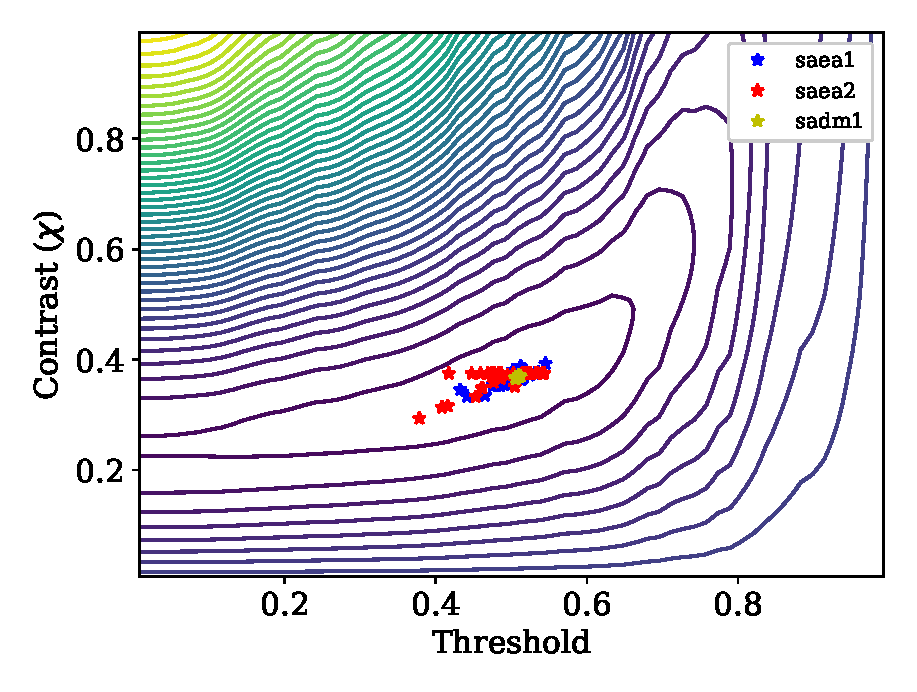
\includegraphics[width=.45\textwidth]{./figuras/casestudy/austria/surface1}\label{fig:results:casestudy:austria:boxplot:surface:1}} \hspace{.05\textwidth}
				\subfloat[]{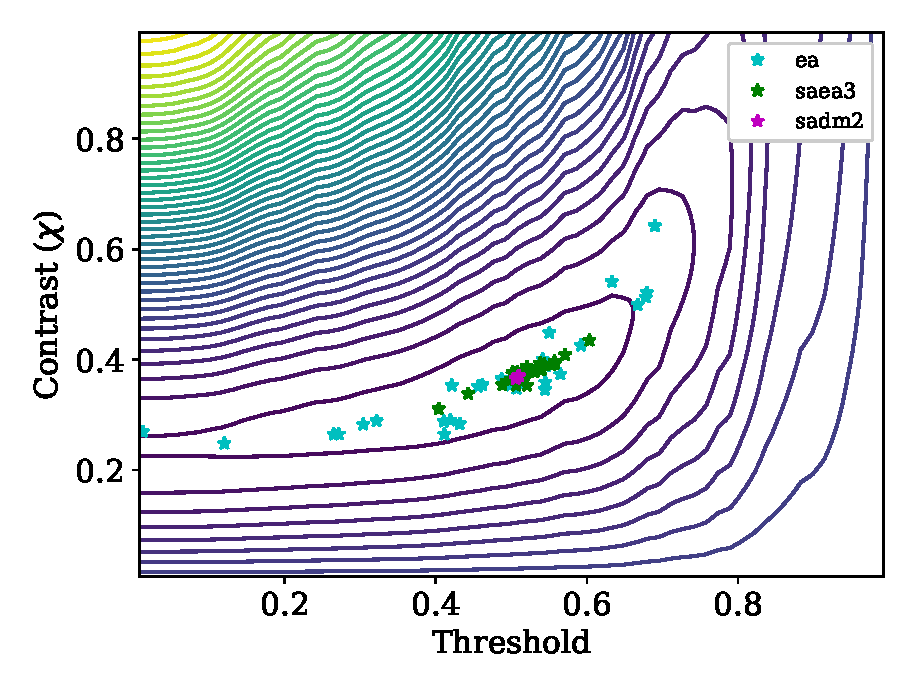
\includegraphics[width=.45\textwidth]{./figuras/casestudy/austria/surface2}\label{fig:results:casestudy:austria:boxplot:surface:2}}
				\caption[Surface of the two-dimensional optimization problem obtained from the transformation of the Austria profile and the final solutions obtained by different algorithms.]{Surface of the two-dimensional optimization problem obtained from the transformation of the Austria profile and the final solutions obtained by different algorithms. Subfigure (a) shows the final solutions obtained by SAEA1, SAEA2, and SADM1 algorithms, while subfigure (b) shows the final solutions obtained by EA, SAEA3, and SADM2 algorithms.}
				\label{fig:results:casestudy:austria:surface}
			\end{figure}
		
			% 1. A Fig. \ref{fig:results:casestudy:austria:surface} mostra a superfície da função-objetivo e a posição das soluções finais encontrada por cada algoritmo baseado na transformação do problema inverso em um de otimização bidimensional.
			% 2. Para uma superfície razoavelmente comportada no sentido macro, os SADM's se comportam como algoritmos determinísticos, uma vez que convergiram todas as vezes para o mesmo ponto.
			% 3. A figura mostra também o grande espalhamento das soluções do EA, indicando que o número de avaliações precisaria ser bem maior para que o algoritmo convergisse mais vezes para o local do ótimo.
			% 4. Os SAEA's tiveram um comportamento similar, exceto talvez pelo SAEA3 que ligeiramente se afastou mais do ponto encontrado pelos SADM's.
			% 5. É importante que soluções finais pouco mais distantes do ótimo podem retornar às vezes um erro menor de estimativa de contraste ou de recuperação de forma. Isso se dá pelo motivo que o ponto de ótimo do problema transformado pode ser um pouco deslocado daquilo que seria o ideal para o processo de limiarização e do valor exato de contraste. Esse deslocamento é intrínseco à estimativa do método qualitativo. Ou seja, a solução ótima do problema transformado não é necessariamente a exata, mas a melhor que posso obter a partir do método qualitativo e minimizando o erro da equação de dados. Por isso, a performance do método qualitativo influencia na posição do ótimo.
			
			Figure \ref{fig:results:casestudy:austria:surface} illustrates the performance of the algorithms, displaying both the objective function surface and the locations of the final solutions obtained by each algorithm after transforming the inverse problem into a two-dimensional optimization problem. The SADMs converged to the same point every time, indicating that they behaved like deterministic algorithms for a reasonably smooth surface in the macro sense. The EA solutions, on the other hand, were widely spread, indicating that the number of evaluations would need to be much higher for the algorithm to converge more often to the optimal location.
			
			The SAEA3 had a similar behavior to EA, which slightly moved away from the point found by the SADMs. However, it is important to note that final solutions that are a little farther from the optimum can sometimes return a smaller error in contrast estimation or shape recovery. This is because the optimal point of the transformed problem can be slightly displaced from what would be ideal for the thresholding process and the exact contrast value. This displacement is intrinsic to the estimation of the qualitative method. That is, the optimal solution of the transformed problem is not necessarily the exact one, but the best that can be obtained from the qualitative method and minimizing the error of the data equation. Therefore, the performance of the qualitative method influences the position of the optimum.
		
		\subsection{Multiple Scatterers}\label{chap:results:casestudy:multiple}
		
			% * Esta subseção discute um estudo de caso que considera múltiplos espalhadores.
			% * Esse tipo de cenário é importante pois permite investigar a capacidade de separar os objetos na imagem.
			% * Além disso, o contraste dos espalhadores será consideravelmente mais alto para explorar ainda mais o potencial da aplicação dos modelos substitutos.
			% * A descrição dos três espalhadores presentes no teste será feita a seguir. 
			% * Os três objetos tem contraste igual a 4.
			% * O raio do círculo é $0.1\lambda_b$ e está centrado nas coordenadas ($L_X/4$, $0$).
			% * O lado do quadrado é $0.2\lambda_b$ e está centrado nas coordenadas ($-L_Y/4$, $-L_X/4$).
			% * O lado do triângulo é $0.2\lambda_b$ e está centrado nas coordenadas ($-L_Y/4$, $L_X/4$).
			% * O DNL do problema ficou em 0.915, o que é perto do limiar 1 para o problema começa a ficar muito não-linear. Não chega a ser tanto um caso de espalhador forte.
			% * Os parâmetros que descrevem os domínios do problema estão presentes na Tabela 2.
			% * Todas as outras configurações de sintetização dos dados do campo espalhado são as mesmas do estudo de caso anterior, exceto que agora a resolução da imagem original é 120$\times$120.
	
			This subsection presents a case study that examines the ability to separate objects in an image when considering multiple scatterers. This type of scenario is significant and, in order to further explore the application potential of the surrogate models, the contrast of the scatterers will be considerably higher. The study describes three scatterers that have a contrast level equal to 4. The radius of the circle is $0.1\lambda_b$ and is centered on coordinates ($L_X/4$, $0$. The side of the square is $0.2\lambda_b$ and is centered on coordinates ($-L_Y/4$, $-L_X/4$), while the side of the triangle is $0.2\lambda_b$ and is centered on coordinates ($-L_Y/4$, $L_X/4$). The instance can be seen in Fig. \ref{fig:results:casestudy:multiple:reconstruction:groundtruth} and it is inspired in an experiment presented in \citep{shah2015fast} and \citep{batista2021quadratic} where the same geometries were considered and different contrast levels. The DNL of the problem was at 0.915, which is close to threshold 1 for the problem to start to get very non-linear. The parameters that describe the problem domains are present in Table \ref{tab:results:casestudy:multiple:configuration}. All other settings for synthesizing the scattered field data are the same as in the previous case study, except now the original image resolution is 120$\times$120.
			
			\begin{table}[!h]
				\centering
				\caption[Parameters for the multiple scatterers case study.]{Parameters for problem specification of the multiple scatterers case study.}
				\rowcolors{1}{gray2}{gray1}
				\begin{tabular}{cccccc}
					$N_M$ & $N_S$ & $\lambda_b$ & $R_O$ & $L_X$, $L_Y$ & $\epsilon_{rb}$ \\
					20 & 20 & 1 [m] & 5 [$\lambda_b$] & 0.8 [$\lambda_b$] & 1
				\end{tabular}
				\label{tab:results:casestudy:multiple:configuration}
			\end{table}
			
			% * A configuração dos algoritmos neste estudo de caso foi bem similar ao caso passado. No entanto, alguns ajustes foram necessários para explorar melhor o comportamento dos algoritmos.
			% * Em relação aos algoritmos baseados na transformação do problema, foram feitas as seguintes modificações.
			% * O limite máximo para a variável de contraste foi aumentado para 7, uma vez que o contraste verdadeiro agora é 4.
			% * Critério de parada: 50 avaliações.
			% * Tamanho da amostra inicial de soluções: 25.
			% * O SAEA2 e o EA consideraram populações com 20 indivíduos.
			% * Em relação aos métodos determinísticos, foram feitas as seguintes modificações.
			% * CGM: 150 iterações.
			% * ECSI: 200 iterações.
			% * DBIM: 4 iterações
			% * BIM: 20 iterações
			% * SOM: 200 iterações e índice de corte igual a 5.
			
			In this case study, the configuration of the algorithms was similar to the previous one, but some adjustments were necessary to explore the behavior of the algorithms more effectively. For the algorithms based on problem transformation, some changes were made, including increasing the maximum limit for the contrast variable to 7 since the true contrast is now 4, setting the stopping criterion to 50 evaluations, and using an initial sample size of 25 solutions. SAEA2 and EA were designed with populations consisting of 20 individuals. As for the deterministic methods, some modifications were made, including 150 iterations for CGM, 200 iterations for ECSI, 4 iterations for DBIM, 20 iterations for BIM, and 200 iterations for SOM, with a cut-off index equal to 5.

			\begin{figure}[!h]
				\centering
				\subfloat[Ground-Truth]{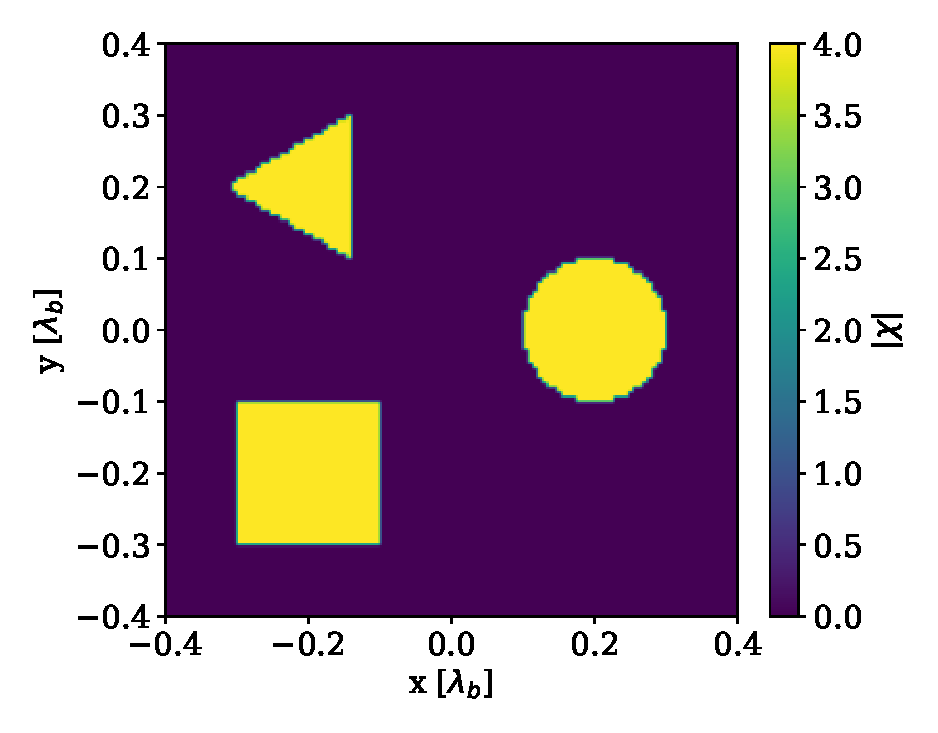
\includegraphics[width=.25\textwidth]{./figuras/casestudy/multiple/groundtruth}\label{fig:results:casestudy:multiple:reconstruction:groundtruth}}
				\subfloat[SAEA1]{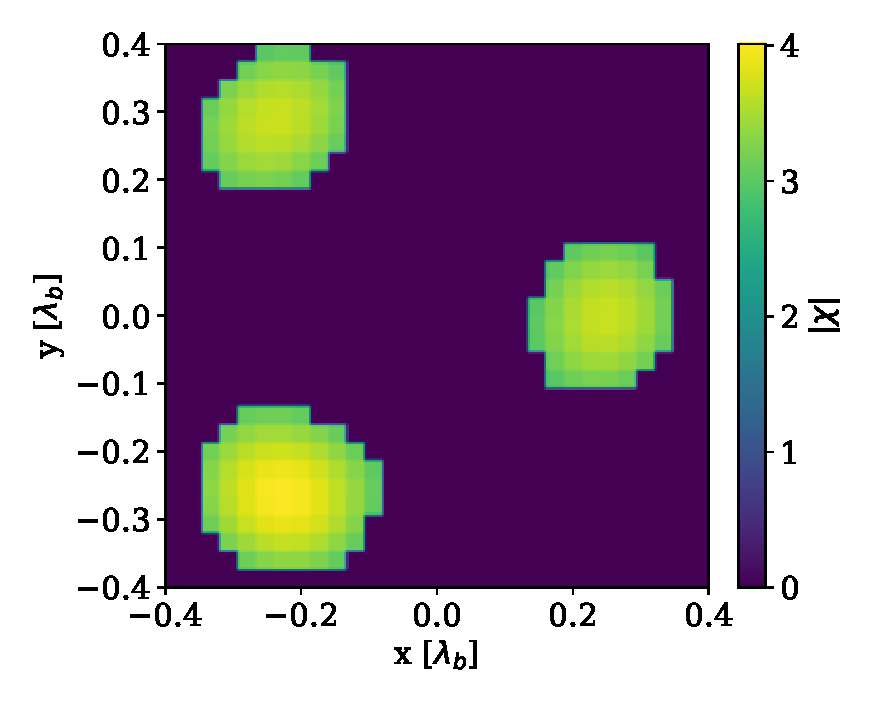
\includegraphics[width=.25\textwidth]{./figuras/casestudy/multiple/reconstruction_saea1}\label{fig:results:casestudy:multiple:reconstruction:saea1}}
				\subfloat[SAEA2]{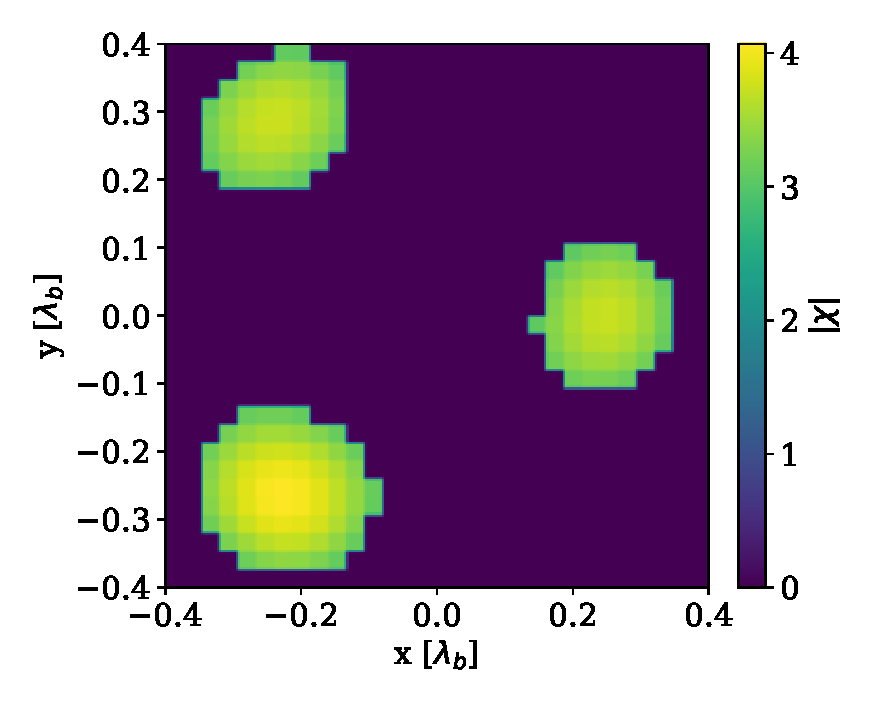
\includegraphics[width=.25\textwidth]{./figuras/casestudy/multiple/reconstruction_saea2}\label{fig:results:casestudy:multiple:reconstruction:saea2}}
				\subfloat[SAEA3]{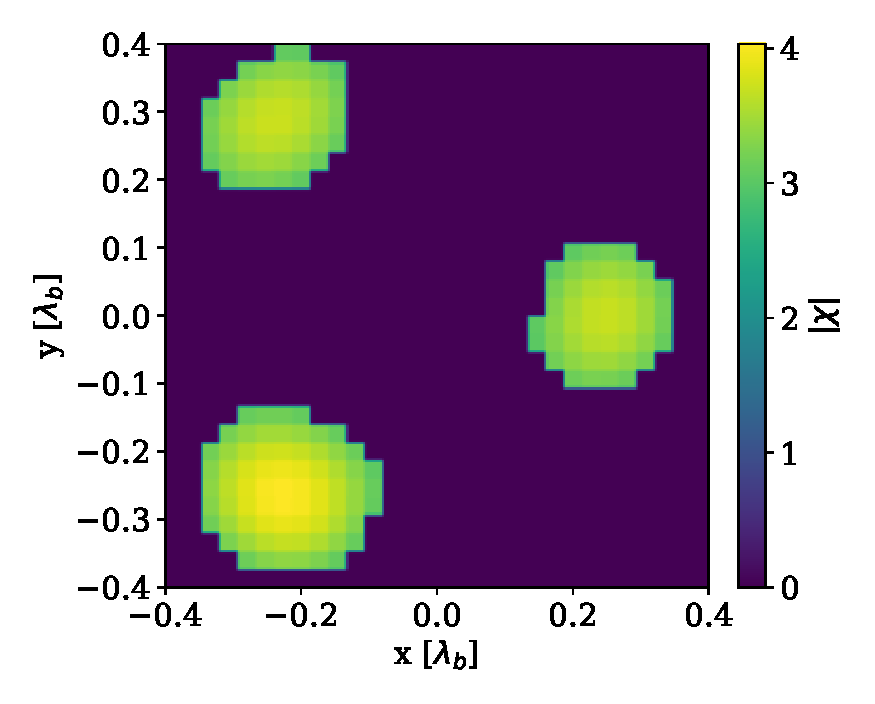
\includegraphics[width=.25\textwidth]{./figuras/casestudy/multiple/reconstruction_saea3}\label{fig:results:casestudy:multiple:reconstruction:saea3}} \\
				\subfloat[SADM1]{\includegraphics[width=.25\textwidth]{./figuras/casestudy/multiple/reconstruction_sadm1}\label{fig:results:casestudy:multiple:reconstruction:sadm1}}
				\subfloat[SADM2]{\includegraphics[width=.25\textwidth]{./figuras/casestudy/multiple/reconstruction_sadm2}\label{fig:results:casestudy:multiple:reconstruction:sadm2}}
				\subfloat[EA]{\includegraphics[width=.25\textwidth]{./figuras/casestudy/multiple/reconstruction_ea}\label{fig:results:casestudy:multiple:reconstruction:ea}}
				\subfloat[BIM]{\includegraphics[width=.25\textwidth]{./figuras/casestudy/multiple/reconstruction_bim}\label{fig:results:casestudy:multiple:reconstruction:bim}} \\
				\subfloat[DBIM]{\includegraphics[width=.25\textwidth]{./figuras/casestudy/multiple/reconstruction_dbim}\label{fig:results:casestudy:multiple:reconstruction:dbim}}
				\subfloat[CGM]{\includegraphics[width=.25\textwidth]{./figuras/casestudy/multiple/reconstruction_cgm}\label{fig:results:casestudy:multiple:reconstruction:cgm}}
				\subfloat[ECSI]{\includegraphics[width=.25\textwidth]{./figuras/casestudy/multiple/reconstruction_ecsi}\label{fig:results:casestudy:multiple:reconstruction:ecsi}}
				\subfloat[SOM]{\includegraphics[width=.25\textwidth]{./figuras/casestudy/multiple/reconstruction_som}\label{fig:results:casestudy:multiple:reconstruction:som}} 
				\caption[Multiple scatterers case study: Comparison of image reconstructions using surrogate model-assisted algorithms and deterministic methods.]{Comparison of image reconstructions using surrogate model-assisted algorithms and deterministic methods considering the multiple scatterers case study: (a) shows the ground-truth image; (b), (c), and (d) depict the best image recovered by SAEA1, SAEA2, and SAEA3, respectively, in 30 execution according to $\zeta_{\epsilon OE}$ indicator; (e), (f) and (g) show the best image recovered by SADM1, SADM2, and EA, respectively, in 30 execution according to $\zeta_{\epsilon OE}$ indicator; (g) shows the image recovered by BIM, and (h) shows the image recovered by DBIM; finally, (i), (k), and (l) show the image recovered by CGM, ECSI, and SOM, respectively.}
				\label{fig:results:casestudy:multiple:reconstruction}
			\end{figure}
		
			% * A Fig. 5.7 apresenta as melhores reconstruções dos algoritmos que foram executados múltiplas vezes seguindo o mesmo critério do estudo de caso passado, assim como as imagens dos métodos determinísticos.
			% * No caso dos algoritmos baseados na transformação do problema, os espalhadores pareceram um pouco mais espaçados em relação ao centro da imagem reconstruída. Tanto é que os espalhadores ficaram muito próximos das bordas da imagem. Mas as melhores estimativas do contraste foram muito boas.
			% * O BIM não teve sucesso detectar os espalhadores.
			% * Na imagem do DBIM parece até haver três espalhadores. Porém, ainda há ondulações muito significativas na região de fundo.
			% * CGM, ECSI e SOM conseguiram fazer detecção de três espalhadores com valores bem próximos do exato. O CGM teve um pouco mais de dificuldade em relação às ondulações no meio de fundo.
			
			The results are presented in Fig. \ref{fig:results:casestudy:multiple:reconstruction}, which displays the best reconstructions of the algorithms that were executed multiple times following the same criteria as the previous case study, along with images of the deterministic methods. In the case of algorithms based on the transformation of the problem (Figs. \ref{fig:results:casestudy:multiple:reconstruction:saea1}-\ref{fig:results:casestudy:multiple:reconstruction:ea}), the scatterers appeared a little more displaced from the center of the reconstructed image, and they were very close to the edges of the image. However, the best estimates of the contrast were excellent. BIM (Fig. \ref{fig:results:casestudy:multiple:reconstruction:bim}) was not successful in detecting the scatterers, while DBIM (Fig. \ref{fig:results:casestudy:multiple:reconstruction:dbim}) displayed significant noise in the background region, even though it might look like there are three scatterers in the image. CGM, ECSI, and SOM (Figs. \ref{fig:results:casestudy:multiple:reconstruction:cgm}-\ref{fig:results:casestudy:multiple:reconstruction:som}) were able to detect three scatterers with values less close to the exact one than the proposed algorithms, although CGM had more difficulty with background noise.
		
			\begin{figure}[!h]
				\centering
				\subfloat[SAEA1]{\includegraphics[width=.25\textwidth]{./figuras/casestudy/multiple/convergence_saea1}\label{fig:results:casestudy:multiple:convergence:saea1}}
				\subfloat[SAEA2]{\includegraphics[width=.25\textwidth]{./figuras/casestudy/multiple/convergence_saea2}\label{fig:results:casestudy:multiple:convergence:saea2}}
				\subfloat[SAEA3]{\includegraphics[width=.25\textwidth]{./figuras/casestudy/multiple/convergence_saea3}\label{fig:results:casestudy:multiple:convergence:saea3}}
				\subfloat[SADM1]{\includegraphics[width=.25\textwidth]{./figuras/casestudy/multiple/convergence_sadm1}\label{fig:results:casestudy:multiple:convergence:sadm1}} \\
				\subfloat[SADM2]{\includegraphics[width=.25\textwidth]{./figuras/casestudy/multiple/convergence_sadm2}\label{fig:results:casestudy:multiple:convergence:sadm2}}
				\subfloat[EA]{\includegraphics[width=.25\textwidth]{./figuras/casestudy/multiple/convergence_ea}\label{fig:results:casestudy:multiple:convergence:ea}}
				\subfloat[BIM]{\includegraphics[width=.25\textwidth]{./figuras/casestudy/multiple/convergence_bim}\label{fig:results:casestudy:multiple:convergence:bim}}
				\subfloat[DBIM]{\includegraphics[width=.25\textwidth]{./figuras/casestudy/multiple/convergence_dbim}\label{fig:results:casestudy:multiple:convergence:dbim}} \\
				\subfloat[CGM]{\includegraphics[width=.25\textwidth]{./figuras/casestudy/multiple/convergence_cgm}\label{fig:results:casestudy:multiple:convergence:cgm}}
				\subfloat[ECSI]{\includegraphics[width=.25\textwidth]{./figuras/casestudy/multiple/convergence_ecsi}\label{fig:results:casestudy:multiple:convergence:ecsi}}
				\subfloat[SOM]{\includegraphics[width=.25\textwidth]{./figuras/casestudy/multiple/convergence_som}\label{fig:results:casestudy:multiple:convergence:som}} 
				\caption[Convergence of the objective function for the multiple scatterers case obtained by the stochastic and deterministic algorithms.]{Convergence of the objective function for the multiple scatterers case obtained by the stochastic and deterministic algorithms. (a) to (k) show the curves obtained by SAEA1, SAEA2, SAEA3, SADM1, SADM2, EA, BIM, DBIM, CGM, ECSI, and SOM algorithms, respectively. The x-axis represents the number of iterations, and the y-axis represents the value of the objective function of the correspondent algorithm.}
				\label{fig:results:casestudy:multiple:convergence}
			\end{figure}
		
			% * A Fig 5.8 mostra a convergência da função objetivo para cada um dos algoritmos.
			% * A convergência dos algoritmos SADM1 e SADM2 foi muito menos homogênea neste estudo de caso. Desta vez, o comportamento foi mais parecido com um algoritmo estocástico, como os SAEAs. Embora as decisões dentro do processo iterativo dos SADMs seja determinísticas, a hipótese é que os processos dentro do treinamento do modelo substituto sejam a causa para as diferenças nas curvas de convergência entre as execuções. E isso se torna mais acentuado em cenários de espalhadores com alto contraste.
			% * As curvas de convergência dos algoritmos SAEAs foram semelhantes às do estudo de caso passado. Nota-se que o SAEA1 tende a ter curvas um pouco mais homogêneas do que o SAEA3 e que, embora o SAEA2 tenha tido apenas 3 gerações, algumas das execuções encontraram soluções com o mesmo valor da função objetivo que as melhores soluções encontradas pelos os outros dois algoritmos.
			% * A convergência dos algoritmos CGM, ECSI e SOM mostram que eles terminaram suas execuções com soluções estáveis. Logo, mesmo se mais iterações fossem dadas, as imagens reconstruídas não iriam diferir significativamente daquelas mostradas nas Figs. 5.7 (j)-(l). Logo, nesta instância, esses algoritmos não iriam conseguir uma reconstrução melhor.
			
			Figure \ref{fig:results:casestudy:multiple:convergence} presents the convergence of the objective function for each algorithm. Interestingly, the convergence of the SADM1 and SADM2 algorithms (Figs. \ref{fig:results:casestudy:multiple:convergence:sadm1}-\ref{fig:results:casestudy:multiple:convergence:sadm2}) was less homogeneous in this case study, behaving more like a stochastic algorithm such as SAEAs. Although the decisions within the iterative process of SADMs are deterministic, the differences in the convergence curves between runs could be due to the processes within the surrogate model training, which can be more complex in high-contrast scattering scenarios.
			
			On the other hand, the convergence curves of the SAEAs algorithms were similar to those of the previous case study. SAEA1 (Fig. \ref{fig:results:casestudy:multiple:convergence:saea1}) had slightly more homogeneous curves than SAEA3 (Fig. \ref{fig:results:casestudy:multiple:convergence:saea3}), and even though SAEA2 (Fig. \ref{fig:results:casestudy:multiple:convergence:saea2}) had only 3 generations, some of the runs found solutions with the same objective function value as the best solutions found by the other two algorithms.
			
			Finally, the convergence of the CGM, ECSI, and SOM algorithms (Figs. \ref{fig:results:casestudy:multiple:convergence:cgm}-\ref{fig:results:casestudy:multiple:convergence:som}) indicates that they finished their runs with stable solutions. Therefore, even if more iterations were given, the reconstructed images would not significantly differ from those shown in Figures \ref{fig:results:casestudy:multiple:reconstruction:cgm}-\ref{fig:results:casestudy:multiple:reconstruction:som}. In this scenario, these algorithms would not obtain a better reconstruction.
		
			\begin{figure}
				\centering
				\includegraphics[width=.9\textwidth]{./figuras/casestudy/multiple/boxplot_zeta_eoe}
				\caption[Performance of $\zeta_{\epsilon OE}$ indicator for various algorithms in the multiple scatterers case study.]{Performance of $\zeta_{\epsilon OE}$ indicator for various algorithms in the multiple scatterers case study. Boxplots show quartiles of 30 executions for stochastic algorithms, and the solid line represents the deterministic algorithms.}
				\label{fig:results:casestudy:multiple:boxplot:zeta_eoe}
			\end{figure}
		
			% * A Fig. 5.9 apresenta os resultados do indicador $\zeta_{\epsilon OE}$ para cada algoritmo.
			% * O CGM foi o algoritmo com menor erro na estimativa do contraste dos objetos, embora a imagem reconstruída como um todo não tenha sido tão boa (Fig. \ref{fig:results:casestudy:multiple:reconstruction:cgm}). Mesmo superestimando o contraste ligeiramente mais que os algoritmos assistidos por modelos substitutos, o erro pode ter sido menor por não exibir o comportamento de afastamento, o que acaba influenciando muito na medida do erro.
			% * Embora a posição da mediana do algoritmo SAEA1 esteja acima das demais dos outros algoritmos assistidos por modelos substitutos, o Kruskal-Wallis H-Test não detecta diferenças na mediana da performance entre todos esses algoritmos (p-valor = 0.655). Logo, não é possível afirmar que alguns desses algoritmos teve uma performance mediana melhor.
			% * Embora as medianas dos algoritmos assistidos por modelos substitutos estejam acima dos valores encontrados pelos métodos SOM, CGM e ECSI, a diferença não chega a ser mais que 20 [\%/pixel].
		
			In Figure \ref{fig:results:casestudy:multiple:boxplot:zeta_eoe}, the results of indicator $\zeta_{\epsilon OE}$ for each algorithm are presented. The CGM algorithm had the lowest error in estimating the contrast of objects, but its reconstructed image was not as satisfactory as the other algorithms (Fig. \ref{fig:results:casestudy:multiple:reconstruction:cgm}). However, even with a slight overestimation of the contrast compared to the surrogate model-assisted algorithms, the error may have been smaller due to the lack of distancing behavior observed for the proposed algorithm and that influences the error measure. The Kruskal-Wallis H-Test did not detect any differences in the median performance between the surrogate model-assisted algorithms, despite SAEA1 having a higher median position. The algorithms assisted by surrogate models had higher medians than the SOM, CGM, and ECSI methods, but the difference did not exceed 20 [\%/pixel].
		
			\begin{figure}
				\centering
				\includegraphics[width=.9\textwidth]{./figuras/casestudy/multiple/boxplot_zeta_s}
				\caption[Performance of shape error estimation quantified by the $\zeta_S$ indicator obtained by the set of algorithms considering the multiple scatterers case study.]{Performance of shape error estimation quantified by the $\zeta_S$ indicator obtained by the set of algorithms considering the multiple scatterers case study. The boxes represent the quartiles of the 30 executions of the stochastic algorithms, while the other points indicate the obtained values by the deterministic ones. The shape error is calculated based on the ground-truth image and the reconstructed image obtained by each algorithm.}
				\label{fig:results:casestudy:multiple:boxplot:zeta_s}
			\end{figure}
			
			% * A Fig. 5.10 apresenta os resultados do indicador X que quantifica a recuperação de forma dos espalhadores pelos algoritmos.
			% * Da mesma maneira como no indicador de erro de estimativa de contraste, o CGM teve o menor erro de recuperação de forma. No entanto, dessa vez, a diferença foi mais significativa chegando a, aproximadamente, 50 [\%] de diferença entre o segundo algoritmo. Ainda assim, vale lembrar que nenhum algoritmo conseguiu reconstruir formas que efetivamente se parecessem com os espalhadores, conforme mostrado na Fig. \ref{fig:results:casestudy:multiple:reconstruction}.
			% * A mediana dos algoritmos assistidos por modelo substituto são bem próximas. No entanto, se compararmos as medianas dos algoritmos SAEA2, SAEA3, SADM1 e SADM2, nenhuma diferença será detectada pelo Kruskal-Wallis H-Test a um nível de significância de 5\% (valor-p = 0.065). No entanto, quando adicionamos o SAEA1 nessa comparação, a performance mediana desse algoritmo será melhor que a dos outros algoritmos (valor-p $<0.001$ em todas as comparações post-hoc). Portanto, o SAEA1 teve uma performance mediana melhor, mas a diferença também não é tão grande e significativa do ponto de vista da imagem reconstruída.
			
			The results of the $\zeta_S$ indicator that evaluates the shape recovery of the scatterers by the algorithms is presented in Fig. \ref{fig:results:casestudy:multiple:boxplot:zeta_s}. The CGM algorithm had the lowest shape recovery error, with a significant difference of around 50 [\%] compared to the second-best algorithm. However, none of the algorithms were able to reconstruct shapes that resembled the scatterers.
			
			Regarding the surrogate model-assisted algorithms, the medians were very close to each other. When comparing the medians of SAEA2, SAEA3, SADM1, and SADM2 algorithms, the Kruskal-Wallis H-Test did not detect any difference at a significance level of 5\% (p-value $= 0.065$). However, when including SAEA1 in the comparison, it showed a better median performance than the other algorithms (p-value $< 0.001$ in all post-hoc comparisons). Nonetheless, the difference is not significant enough from the point of view of the reconstructed image.
			
			\begin{figure}
				\centering
				\includegraphics[width=.9\textwidth]{./figuras/casestudy/multiple/boxplot_time}
				\caption[Box plot showing the execution time distribution of the set of algorithms considered for the multiple scatterers case study.]{Box plot showing the execution time distribution of the set of algorithms considered for the multiple scatterers case study. The boxes represent the quartiles of the 30 executions of the stochastic algorithms, and the whiskers represent the minimum and maximum values. The deterministic algorithms are represented by individual points. The execution time results are presented in seconds.}
				\label{fig:results:casestudy:multiple:boxplot:time}
			\end{figure}
		
			% * A Fig. 5.11 apresenta os resultados do tempo de execução dos algoritmos.
			% * O tempo de execução do BIM e do DBIM foi menor tendo em vista que poucas iterações foram necessárias, e assim, o cálculo mais custoso foi menos vezes acionado durante a execução do algoritmo.
			% * A performance mediana dos algoritmos SADM2 e EA foram muito semelhantes, de modo que não foi detectada diferença segundo o Welch Two Sample T-Test (valor-p = 0.203). No entanto, a mediana destes dois estão abaixo dos demais algoritmos.
			% * Levando em consideração este indicador junto com os indicadores $\zeta_{\epsilon OE}$ e $\zeta_S$, a escolha entre SADM2 e o CGM nesta instância pode ser entendida como uma troca entre qualidade da reconstrução e tempo de execução. Em outras palavras, o SADM2 pode não alcançar a mesma performance que o CGM nos indicadores de forma e estimativa de contraste, mas consegue alcançar valores não tão maiores por um tempo bem menor.
			
			Figure \ref{fig:results:casestudy:multiple:boxplot:time} displays the results of the execution time of the algorithms. BIM and DBIM had shorter execution times since fewer iterations were needed, which means the most expensive calculation was called fewer times during the algorithm execution. The median performances of the SADM2 and EA algorithms were quite similar, and no significant difference was detected based on the Welch Two Sample T-Test (p-value = 0.203). However, the medians of these two algorithms were below that of the other algorithms. By considering this indicator along with the $\zeta_{\epsilon OE}$ and $\zeta_S$ indicators, choosing between SADM2 and CGM in this case could be seen as a trade-off between reconstruction quality and execution time. In other words, while SADM2 may not achieve the same performance as CGM in shape and contrast estimation indicators, it can achieve slightly higher values in a much shorter time.
		
			\begin{figure}
				\centering
				\subfloat[]{\includegraphics[width=.45\textwidth]{./figuras/casestudy/multiple/surface1}\label{fig:results:casestudy:multiple:boxplot:surface:1}} \hspace{.05\textwidth}
				\subfloat[]{\includegraphics[width=.45\textwidth]{./figuras/casestudy/multiple/surface2}\label{fig:results:casestudy:multiple:boxplot:surface:2}}
				\caption[Surface of the two-dimensional optimization problem obtained from the transformation of the multiple scatterers case study and the final solutions obtained by different algorithms.]{Surface of the two-dimensional optimization problem obtained from the transformation of the multiple scatterers case study and the final solutions obtained by different algorithms. Subfigure (a) shows the final solutions obtained by SAEA1, SAEA2, and SADM1 algorithms, while subfigure (b) shows the final solutions obtained by EA, SAEA3, and SADM2 algorithms.}
				\label{fig:results:casestudy:multiple:surface}
			\end{figure}
		
			% * A Fig. 5.12 exibe a superfície da função objetivo resultante da transformação em um problema de otimização bidimensional e a localização das soluções finais encontradas pelos algoritmos nas múltiplas execuções.
			% * Com o aumento da não-linearidade do problema, a superfície ficou menos convexa.
			% * Além disso, a imagem também mostra um certo agrupamento de soluções em torno do ponto ($T$, $\chi$) $=$ (0.75, 4) e outro menor em torno de (0.8, 5). Pode ser que este último seja um mínimo local onde algumas das execuções poderiam ter ficado presas. A ocorrência de mínimos locais mais difíceis de escapar pode ser mais comum a medida que o problema vai ficando mais não-linear ou o contraste dos espalhadores vai subindo.
			% * As soluções finais encontradas de todos algoritmos ficaram espalhadas sendo que apenas no caso do EA é que houveram soluções fora da região de subnível mais baixa.
		
			Figure \ref{fig:results:casestudy:multiple:surface} presents the surface of the objective function resulting from the transformation in a two-dimensional optimization problem, along with the location of the final solutions found by the algorithms in multiple runs. As the nonlinearity of the problem increased, the surface became less convex, and there was a certain grouping of solutions around the point $T$, $\chi$) $=$ (0.75, 4) and a smaller one around (0.8, 5). It is possible that the latter is a local minimum where some of the runs may have gotten stuck. The occurrence of more difficult to escape local minima may be more common as the problem becomes more non-linear or the contrast of the scatterers increases. The final solutions found for all algorithms were scattered, and only in the case of EA that solutions outside the lowest sublevel region were returned.
		
		\subsection{Non-Homogeneous Scatterer}\label{chap:results:casestudy:nonhomogeneous}
		
			% * The thrid case study considers a nonhomogeneous scatterer.
			% * This scenario is relevant since OSM is qualitative method that allows to identify different levels of contrast.
			% * The case study is inspired in an experiment presented in \citep{bevacqua2021effective}.
			% * The scatterer is a square which side is $\lambda_b$. Within the square, there are three regions where the contrast is 0.4, 0.9, and 1.25.
			% * Further information regarding the scatterer specification can be found in the mentioned reference.
			% * The Table 3 shows the specifications for measurement and imaging domains.
			% * The Degree of Non-Linearity for this case is 1.396, which is above the threshold for cases that the Born Approximation may be applied.
			% * The scatterer is illustrated in Figure 5.13 (a).
			% * All settings for synthesizing the scattered field data are the same as in the previous case study.
			
			The third case study presented in this work focuses on the imaging of a nonhomogeneous scatterer, which is a square of side length equals to $\lambda_b$ with three different regions of contrast (0.4, 0.9, and 1.25) inside it. This scenario is relevant because it allows the qualitative identification of different levels of contrast using the OSM method. The inspiration for this study comes from a similar experiment presented by \cite{bevacqua2020physical}. The scatterer's detailed specifications can be found in the reference. Table \ref{tab:results:casestudy:nonhomogeneous:configuration} provides the specifications for measurement and imaging domains. Figure \ref{fig:results:casestudy:nonhomogeneous:reconstruction:groundtruth} illustrates the scatterer. The degree of non-linearity for this case is 1.396, which is above the threshold for cases where the Born Approximation can be applied. All settings for synthesizing the scattered field data are the same as in the previous case study.
			
			\begin{table}[!h]
				\centering
				\caption[Parameters for the nonhomogeneous scatterer case study.]{Parameters for problem specification of the nonhomogeneous scatterer case study.}
				\rowcolors{1}{gray2}{gray1}
				\begin{tabular}{cccccc}
					$N_M$ & $N_S$ & $\lambda_b$ & $R_O$ & $L_X$, $L_Y$ & $\epsilon_{rb}$ \\
					16 & 16 & 1 [m] & 3.33 [$\lambda_b$] & 1.67 [$\lambda_b$] & 1
				\end{tabular}
				\label{tab:results:casestudy:nonhomogeneous:configuration}
			\end{table}
			
			For this case study, adjustments were made to the algorithm configurations to more effectively explore their behavior. For the problem transformation-based algorithms, the maximum limit for the contrast variable was reduced to 3 since the maximum contrast in the true image is now 1.25. The stopping criterion was set to 60 evaluations. SAEA2 and EA utilized populations of 20 individuals as in the previous case study. Deterministic methods also underwent some modifications, such as CGM and ECSI using 50 iterations, DBIM using 3 iterations, BIM using 15 iterations, and SOM using 500 iterations with a cut-off index of 5.
		
			\begin{figure}[!h]
				\centering
				\subfloat[Ground-Truth]{\includegraphics[width=.25\textwidth]{./figuras/casestudy/nonhomogeneous/groundtruth}\label{fig:results:casestudy:nonhomogeneous:reconstruction:groundtruth}}
				\subfloat[SAEA1]{\includegraphics[width=.25\textwidth]{./figuras/casestudy/nonhomogeneous/reconstruction_saea1}\label{fig:results:casestudy:nonhomogeneous:reconstruction:saea1}}
				\subfloat[SAEA2]{\includegraphics[width=.25\textwidth]{./figuras/casestudy/nonhomogeneous/reconstruction_saea2}\label{fig:results:casestudy:nonhomogeneous:reconstruction:saea2}}
				\subfloat[SAEA3]{\includegraphics[width=.25\textwidth]{./figuras/casestudy/nonhomogeneous/reconstruction_saea3}\label{fig:results:casestudy:nonhomogeneous:reconstruction:saea3}} \\
				\subfloat[SADM1]{\includegraphics[width=.25\textwidth]{./figuras/casestudy/nonhomogeneous/reconstruction_sadm1}\label{fig:results:casestudy:nonhomogeneous:reconstruction:sadm1}}
				\subfloat[SADM2]{\includegraphics[width=.25\textwidth]{./figuras/casestudy/nonhomogeneous/reconstruction_sadm2}\label{fig:results:casestudy:nonhomogeneous:reconstruction:sadm2}}
				\subfloat[EA]{\includegraphics[width=.25\textwidth]{./figuras/casestudy/nonhomogeneous/reconstruction_ea}\label{fig:results:casestudy:nonhomogeneous:reconstruction:ea}}
				\subfloat[BIM]{\includegraphics[width=.25\textwidth]{./figuras/casestudy/nonhomogeneous/reconstruction_bim}\label{fig:results:casestudy:nonhomogeneous:reconstruction:bim}} \\
				\subfloat[DBIM]{\includegraphics[width=.25\textwidth]{./figuras/casestudy/nonhomogeneous/reconstruction_dbim}\label{fig:results:casestudy:nonhomogeneous:reconstruction:dbim}}
				\subfloat[CGM]{\includegraphics[width=.25\textwidth]{./figuras/casestudy/nonhomogeneous/reconstruction_cgm}\label{fig:results:casestudy:nonhomogeneous:reconstruction:cgm}}
				\subfloat[ECSI]{\includegraphics[width=.25\textwidth]{./figuras/casestudy/nonhomogeneous/reconstruction_ecsi}\label{fig:results:casestudy:nonhomogeneous:reconstruction:ecsi}}
				\subfloat[SOM]{\includegraphics[width=.25\textwidth]{./figuras/casestudy/nonhomogeneous/reconstruction_som}\label{fig:results:casestudy:nonhomogeneous:reconstruction:som}} 
				\caption[Nonhomogeneous scatterer case study: Comparison of image reconstructions using surrogate model-assisted algorithms and deterministic methods.]{Comparison of image reconstructions using surrogate model-assisted algorithms and deterministic methods considering the nonhomogeneous scatterer case study: (a) shows the ground-truth image; (b), (c), and (d) depict the best image recovered by SAEA1, SAEA2, and SAEA3, respectively, in 30 execution according to $\zeta_{\epsilon OE}$ indicator; (e), (f) and (g) show the best image recovered by SADM1, SADM2, and EA, respectively, in 30 execution according to $\zeta_{\epsilon OE}$ indicator; (g) shows the image recovered by BIM, and (h) shows the image recovered by DBIM; finally, (i), (k), and (l) show the image recovered by CGM, ECSI, and SOM, respectively.}
				\label{fig:results:casestudy:nonhomogeneous:reconstruction}
			\end{figure}
		
			% * A Fig. 5.13 apresenta as melhores reconstruções dos algoritmos que foram executados múltiplas vezes seguindo o mesmo critério do estudo de caso passado, assim como as imagens dos métodos determinísticos.
			% * As imagens reconstruídas pelos algoritmos propostos são bem semelhantes entre si, i.e., parecem ser reconstruídas a partir do mesmo nível de limiar e de estimativa de contraste. O nível mais baixo de contraste do espalhador parece estar proporcionalmente mais alto do que na imagem original, que modo que este nível se confunde um pouco com o segundo. Isto tem a ver com a performance do método qualitativo neste tipo de cenário, i.e., o OSM pode ter uma certa dificuldade de estimar bem as diferenças quando essas começam a ficar distante uma das outras. Possivelmente por causa disso é que o contraste ficou subestimado em todos os resultados, uma vez que o erro da equação de dados poderia crescer muito se a média de contraste no espalhador subisse para que o máximo valor alcançasse o valor verdadeiro.
			% * O BIM fez uma boa reconstrução. No resultado obtido por ele, o contorno do espalhador ficou levemente destacado e os níveis de contraste bem estimados. Já o DBIM não teve uma resultado tão bom assim.
			% * CGM e ECSI até realizaram reconstruções cujo o formato do espalhador até se assemelha ao verdadeiro. No entanto, no CGM, o contraste foi superestimado e, no ECSI, a região de contraste mais alto ficou um pouco distorcida.
			% * O SOM não realizou uma boa reconstrução. Possivelmente porque o nível de ruído pode ter afetado muito o desempenho do método nesse tipo de cenário.
			
			Figure \ref{fig:results:casestudy:nonhomogeneous:reconstruction} presents the best reconstructions of the algorithms executed multiple times under the same criteria as the previous case study, as well as the images of the deterministic methods. The reconstructed images by the proposed algorithms (Figs. \ref{fig:results:casestudy:nonhomogeneous:reconstruction:saea1}-\ref{fig:results:casestudy:nonhomogeneous:reconstruction:ea}) were very similar to each other, suggesting that they were reconstructed from the same threshold level and contrast estimation. However, the lowest level of contrast in the scatterer appeared to be proportionately higher than in the original image, resulting in a relatively blurred image with the second level. This may be attributed to the difficulty of the OSM method in estimating differences when they become distant from each other. As a result, the contrast was underestimated in all results since the increment in the contrast multiplication factor would represent an object with a higher average contrast and a higher erro in the data equation.
			
			BIM had a satisfactory reconstruction with a notable contour of the scatterer and well-estimated contrast levels. On the other hand, DBIM did not perform well. CGM and ECSI performed reconstructions that resembled the real scatterer, but with some distortions. In CGM, the contrast was overestimated, and in ECSI, the highest contrast region was slightly distorted. Finally, SOM did not perform well, possibly because the noise level greatly affected its performance in this scenario.
		
			\begin{figure}[!h]
				\centering
				\subfloat[SAEA1]{\includegraphics[width=.25\textwidth]{./figuras/casestudy/nonhomogeneous/convergence_saea1}\label{fig:results:casestudy:nonhomogeneous:convergence:saea1}}
				\subfloat[SAEA2]{\includegraphics[width=.25\textwidth]{./figuras/casestudy/nonhomogeneous/convergence_saea2}\label{fig:results:casestudy:nonhomogeneous:convergence:saea2}}
				\subfloat[SAEA3]{\includegraphics[width=.25\textwidth]{./figuras/casestudy/nonhomogeneous/convergence_saea3}\label{fig:results:casestudy:nonhomogeneous:convergence:saea3}}
				\subfloat[SADM1]{\includegraphics[width=.25\textwidth]{./figuras/casestudy/nonhomogeneous/convergence_sadm1}\label{fig:results:casestudy:nonhomogeneous:convergence:sadm1}} \\
				\subfloat[SADM2]{\includegraphics[width=.25\textwidth]{./figuras/casestudy/nonhomogeneous/convergence_sadm2}\label{fig:results:casestudy:nonhomogeneous:convergence:sadm2}}
				\subfloat[EA]{\includegraphics[width=.25\textwidth]{./figuras/casestudy/nonhomogeneous/convergence_ea}\label{fig:results:casestudy:nonhomogeneous:convergence:ea}}
				\subfloat[BIM]{\includegraphics[width=.25\textwidth]{./figuras/casestudy/nonhomogeneous/convergence_bim}\label{fig:results:casestudy:nonhomogeneous:convergence:bim}}
				\subfloat[DBIM]{\includegraphics[width=.25\textwidth]{./figuras/casestudy/nonhomogeneous/convergence_dbim}\label{fig:results:casestudy:nonhomogeneous:convergence:dbim}} \\
				\subfloat[CGM]{\includegraphics[width=.25\textwidth]{./figuras/casestudy/nonhomogeneous/convergence_cgm}\label{fig:results:casestudy:nonhomogeneous:convergence:cgm}}
				\subfloat[ECSI]{\includegraphics[width=.25\textwidth]{./figuras/casestudy/nonhomogeneous/convergence_ecsi}\label{fig:results:casestudy:nonhomogeneous:convergence:ecsi}}
				\subfloat[SOM]{\includegraphics[width=.25\textwidth]{./figuras/casestudy/nonhomogeneous/convergence_som}\label{fig:results:casestudy:nonhomogeneous:convergence:som}} 
				\caption[Convergence of the objective function for the nonhomogeneous scatterer case obtained by the stochastic and deterministic algorithms.]{Convergence of the objective function for the nonhomogeneous scatterer case obtained by the stochastic and deterministic algorithms. (a) to (k) show the curves obtained by SAEA1, SAEA2, SAEA3, SADM1, SADM2, EA, BIM, DBIM, CGM, ECSI, and SOM algorithms, respectively. The x-axis represents the number of iterations, and the y-axis represents the value of the objective function of the correspondent algorithm.}
				\label{fig:results:casestudy:nonhomogeneous:convergence}
			\end{figure}
		
			% * A Fig. 5.14 mostra as curvas de convergência da função objetivo para os algoritmos considerados.
			% * Os algoritmos SADM1 e SADM2 tiveram leves variações entre as execuções.
			% * Embora o SAEA2 tenha tido 3 gerações, algumas das execuções conseguiram a chegar em soluções com valores de função objetivo baixos como as soluções finais de SAEA1 e SAEA3.
			% * BIM, CGM, ECSI e SOM terminaram suas execuções após alcançarem um nível razoável de estabilidade no processo de convergência. Portanto, mais iterações não iriam mudar muito em a qualidade das imagens reconstruídas.
			
			Figure \ref{fig:results:casestudy:nonhomogeneous:convergence} presents the convergence curves of the considered algorithms in this study. The figure shows that BIM, CGM, ECSI, and SOM reached a reasonable level of stability in the convergence process and ended their executions, indicating that further iterations would not significantly improve the quality of the reconstructed images. Meanwhile, SADM1 and SADM2 had slight variations between runs, and although SAEA2 had 3 generations, some of the runs were able to arrive at solutions with low objective function values like the final solutions of SAEA1 and SAEA3.
		
			\begin{figure}
				\centering
				\includegraphics[width=.9\textwidth]{./figuras/casestudy/nonhomogeneous/boxplot_zeta_eoe}
				\caption[Performance of $\zeta_{\epsilon OE}$ indicator for various algorithms in the nonhomogeneous scatterer case study.]{Performance of $\zeta_{\epsilon OE}$ indicator for various algorithms in the nonhomogeneous scatterer case study. Boxplots show quartiles of 30 executions for stochastic algorithms, and the solid line represents the deterministic algorithms.}
				\label{fig:results:casestudy:nonhomogeneous:boxplot:zeta_eoe}
			\end{figure}
		
			% * A Figura 5.15 mostra os resultados do indicador X obtidos pelos algoritmos.
			% * Embora a imagem reconstruída pelo BIM tenha sido a mais satisfatória, o menor erro de estimativa de contraste foi obtido pelo ECSI. Embora a forma tenha ficado um pouco distorcida, a estimativa em cada píxel pelo ECSI foi melhor.
			% * As medianas da performance dos algoritmos propostos foram bem similares e o Kruskal-Wallis H-Test falha em rejeitar a hipótese de igualdade entre elas (valor-p = 0.08). A diferença entre a performance deles e o ECSI foi, aproximadamente, 3 [%/pixel], o que não é tão ruim.
			
			The performance of the algorithms regarding the contrast estimation in the scatterer area was analyzed based on the results of indicator $\zeta_{\epsilon OE}$ presented in Figure \ref{fig:results:casestudy:nonhomogeneous:boxplot:zeta_eoe}. Despite the fact that the image reconstructed by BIM was the most satisfactory, with a well-estimated contrast and reasonably clear scatterer contour, ECSI was the algorithm with the lowest contrast estimation error, although the shape was slightly distorted. Nevertheless, the difference in performance between BIM and ECSI was not significant, with approximately 1 [\%/pixel]. The performance medians of the proposed algorithms were very similar, and the Kruskal-Wallis H-Test failed to reject the hypothesis of equality between them (p-value $= 0.08$). The performance difference between the proposed algorithms and ECSI was not too large, at around 3 [\%/pixel].
		
			\begin{figure}
				\centering
				\includegraphics[width=.9\textwidth]{./figuras/casestudy/nonhomogeneous/boxplot_zeta_s}
				\caption[Performance of shape error estimation quantified by the $\zeta_S$ indicator obtained by the set of algorithms considering the nonhomogeneous scatterer case study.]{Performance of shape error estimation quantified by the $\zeta_S$ indicator obtained by the set of algorithms considering the nonhomogeneous scatterer study. The boxes represent the quartiles of the 30 executions of the stochastic algorithms, while the other points indicate the obtained values by the deterministic ones. The shape error is calculated based on the ground-truth image and the reconstructed image obtained by each algorithm.}
				\label{fig:results:casestudy:nonhomogeneous:boxplot:zeta_s}
			\end{figure}
		
			% * A Figura 5.15 mostra os resultados do indicador X obtidos pelos algoritmos.
			% * Os algoritmos propostos tiveram uma performance melhor que os métodos determinísticos.
			% * O desempenho ruim do BIM neste indicador pode estar relacionado à dificuldade da aplicação do indicador em imagens muito heterogêneas. Para os algoritmos propostos, este indicador pode ter sido mais baixo por causa da menor heterogeneidade do espalhador e diferença em relação ao meio de fundo.
			% * Entre os algoritmos assistidos por modelos substituto, não há evidências para diferença na performance mediana do indicador, conforme o Kruskal-Wallis H-Test (valor-p = 0.088).
			
			Figure \ref{fig:results:casestudy:nonhomogeneous:boxplot:zeta_s} shows the results obtained by the algorithms considering the $\zeta_S$ indicator. It was observed that the proposed algorithms outperformed the deterministic methods in terms of this indicator. However, it is interesting to note that BIM performed relatively worse than the other proposed algorithms, and this may be related to the difficulty of applying the indicator to significantly heterogeneous images. On the other hand, the proposed algorithms performed better possibly due to the smaller heterogeneity of the scatterer and the difference in respect to the background medium. Among the surrogate model-assisted algorithms, there was no evidence of a significant difference in the median performance of the indicator, as confirmed by the Kruskal-Wallis H-Test (p-value $= 0.088$). This suggests that the performance of the proposed algorithms in terms of this indicator is similar, and none of them stands out significantly from the others.
		
			\begin{figure}
				\centering
				\includegraphics[width=.9\textwidth]{./figuras/casestudy/nonhomogeneous/boxplot_time}
				\caption[Box plot showing the execution time distribution of the set of algorithms considered for the nonhomogeneous scatterer case study.]{Box plot showing the execution time distribution of the set of algorithms considered for the nonhomogeneous scatterer case study. The boxes represent the quartiles of the 30 executions of the stochastic algorithms, and the whiskers represent the minimum and maximum values. The deterministic algorithms are represented by individual points. The execution time results are presented in seconds.}
				\label{fig:results:casestudy:nonhomogeneous:boxplot:time}
			\end{figure}
		
			% * A Figura 5.17 mostra os resultados para o tempo de execução dos algoritmos.
			% * O DBIM teve o menor tempo, uma vez que o número de iterações foi bem baixo.
			% * Em seguida, o BIM obteve o segundo menor tempo. Logo, o BIM consegue em um tempo razoavelmente pequeno, reconstruir a imagem adequadamente.
			% * Alguns dos algoritmos propostos (SAEA2, SADM1, SADM2 e EA) tiveram tempos de execução menor que algoritmos com o SOM e o CGM.
			
			Figure \ref{fig:results:casestudy:nonhomogeneous:boxplot:time} displays the running time of the algorithms analyzed in the study. As expected, some of the deterministic methods required less computational time than the proposed algorithms that use surrogate models. Among them, DBIM had the shortest time, thanks to the low number of iterations in which it can run without diverging. The second shortest time was taken by BIM, which was able to reconstruct the image adequately in a reasonably short time. Among the proposed algorithms, some executions had shorter times than others. Specifically, SAEA2, SADM1, SADM2, and EA required less time than SOM and CGM.
		
			\begin{figure}
				\centering
				\subfloat[]{\includegraphics[width=.45\textwidth]{./figuras/casestudy/nonhomogeneous/surface1}\label{fig:results:casestudy:nonhomogeneous:boxplot:surface:1}} \hspace{.05\textwidth}
				\subfloat[]{\includegraphics[width=.45\textwidth]{./figuras/casestudy/nonhomogeneous/surface2}\label{fig:results:casestudy:nonhomogeneous:boxplot:surface:2}}
				\caption[Surface of the two-dimensional optimization problem obtained from the transformation of the nonhomogeneous scatterer case study and the final solutions obtained by different algorithms.]{Surface of the two-dimensional optimization problem obtained from the transformation of the nonhomogeneous scatterer case study and the final solutions obtained by different algorithms. Subfigure (a) shows the final solutions obtained by SAEA1, SAEA2, and SADM1 algorithms, while subfigure (b) shows the final solutions obtained by EA, SAEA3, and SADM2 algorithms.}
				\label{fig:results:casestudy:nonhomogeneous:surface}
			\end{figure}
			
			% * Figure \ref{fig:results:casestudy:nonhomogeneous:surface} presents the surface of the objective function resulting from the transformation in a two-dimensional optimization problem, along with the location of the final solutions found by the algorithms in multiple runs.
			% * A superfície da função objetivo é semelhante à obtida no estudo de caso do perfil Austria.
			% * Somente o algoritmo EA não teve todas as soluções finais dentro da região de subnível com menor valor no gráfico.
			% * As soluçõe finais dos SADMs ficaram mais concentradas, como era de se esperar por causa dos seus respectivos gráficos de convergência.
			
			Figure \ref{fig:results:casestudy:nonhomogeneous:surface} shows the surface of the objective function along with the location of the final solutions found by the algorithms in multiple runs. The surface of the objective function is similar to that obtained in the Austria profile case study (Fig. \ref{fig:results:casestudy:austria:surface}). The figure shows that only EA did not have all the final solutions within the sublevel region with the lowest value in the graph. This suggests that the EA algorithm may not be as efficient as the other algorithms in finding the optimal solutions. In contrast, the final solutions of the SADMs were more concentrated, as expected because of their respective convergence graphs.
		
		\subsection{Strong Scatterer}\label{chap:results:casestudy:strong}
		
			% 1. O último estudo de caso é a reconstrução de um espalhador forte.
			% 2. O objetivo é demonstrar a aplicabilidade da metodologia proposta em um cenário mais difícil onde geralmente os métodos tradicionais não são capazes de reconstruir.
			% 3. O espalhador considerado é um estrela de 5 pontas cujo o raio do centro até o vértice mais distante vale, aproximadamente, 0.4$\lambda_b$.
			% 4. O contraste do objeto foi definido em 4.
			% 5. As informações sobre os domínios de medição e imageamento estão na Tabela \ref{tab:results:casestudy:strong:configuration}.
			% 6. A resolução da imagem utilizada para sintetização dos dados foi 120$\times$120.
			% 7. O aumento da resolução foi definido para diminuir erros na sintetização do campo espalhado do problema.
			% 8. Outros parâmetros para sintetização dos dados foram os mesmos dos estudos de caso anteriores.
			% 9. O Grau de Não-Linearidade (DNL) para este problema vale 7.39, o que é bem alto.
			
			In the final case study, we explore the reconstruction of a strong scatterer, aiming to showcase the applicability of the proposed methodology in a more challenging scenario where traditional methods often struggle. The scatterer in focus is a 5-pointed star with a radius from the center to the farthest vertex approximately 0.4$\lambda_b$ (see Fig. \ref{fig:results:casestudy:strong:reconstruction:groundtruth}). To emphasize the difficulty, the object contrast has been set to 4, making it even more challenging to accurately reconstruct. Detailed information about the measurement and imaging domains can be found in Table \ref{tab:results:casestudy:strong:configuration}, providing essential specifications for the experimental setup.
			
			To ensure higher precision in data synthesis, we increased the image resolution to 120$\times$120. This resolution enhancement was chosen to minimize errors during the synthesis of the scattered field, considering the complexity of the problem at hand. Other parameters for data synthesis remained consistent with those used in the previous case studies.
			
			The DNL for this particular problem is notably high, measuring 7.39. Such a high DNL value indicates the significant nonlinearity of the problem, further accentuating the challenge in accurately reconstructing the strong scatterer. The combination of the intricate scatterer shape and the high object contrast poses a substantial test for the proposed methodology.
		
			\begin{table}[!h]
				\centering
				\caption[Parameters for the strong scatterer case study.]{Parameters for problem specification of the strong scatterer case study.}
				\rowcolors{1}{gray2}{gray1}
				\begin{tabular}{cccccc}
					$N_M$ & $N_S$ & $\lambda_b$ & $R_O$ & $L_X$, $L_Y$ & $\epsilon_{rb}$ \\
					50 & 50 & 1 [m] & 5 [$\lambda_b$] & 1 [$\lambda_b$] & 1
				\end{tabular}
				\label{tab:results:casestudy:strong:configuration}
			\end{table}
			
			% * Alguns ajustes nos parâmetros de funcionamento dos algoritmos assistidos por modelo substituto foram necessários. Essa mudanças contemplam o aumento da dificuldade do problema por este ser mais não-linear.
			% * O limite máximo da variável de contraste foi ajustado para 7.
			% * O número máximo de iterações do MoM-CG-FFT na avaliação de soluções foi mantido em 20, mesmo que neste cenário isso represente um erro maior na aproximação do campo. Esse número foi mantido para demonstrar que a metodologia não precisa de um cálculo de campo tão preciso mesmo nos cenários mais difíceis.
			% * O número máximo de avaliações, o qual funciona como critério de parada, foi aumentado para 80.
			% * O número de soluções na amostra inicial foi aumentado para 36.
			% * Todas essas mudanças aumentam o custo computacional mas são um reflexo do aumento da complexidade do problema.
			% * Outros parâmetros permanecem como no estudo anterior.
			% * Em relação aos métodos determinísticos, alguns ajustes também foram necessários.
			% * O número máximo de iterações do SOM e do CGM foi ajustado para 1000.
			% * O número máximo de iterações do ECSI foi ajustado para 50.
			% * O número de iterações do BIM foi 4.
			% * O número  de iterações do DBIM foi 2.
			% * Outros parâmetros permanecem como no estudo anterior.
			
			In order to tackle the increased complexity of the problem, several adjustments were made to the operating parameters of both the surrogate model-assisted algorithms and the deterministic methods. These modifications aimed to enhance the performance and adaptability of the algorithms to the more nonlinear nature of the scenario.
			
			For the surrogate model-assisted algorithms, the upper bound of the contrast variable was set to 7, reflecting the higher contrast range present in the problem. Additionally, the maximum number of iterations for the MoM-CG-FFT in the evaluation of solutions remained at 20, despite this representing a greater error in the field approximation. This choice was deliberate to showcase the methodology's robustness even in challenging scenarios, where highly precise field calculations are not necessary. Furthermore, the maximum number of evaluations, serving as a stopping criterion, was increased to 80. To provide a more comprehensive initial sample, the number of solutions was increased to 36. These adjustments, while increasing the computational cost, were essential to address the growing complexity of the problem and obtain accurate results.
			
			The remaining parameters for the surrogate model-assisted algorithms remained consistent with the previous study, ensuring continuity and comparability. Similarly, adjustments were made to the deterministic methods. For SOM and CGM, the maximum number of iterations was extended to 1000, allowing for more comprehensive convergence. ECSI iterations were adjusted to 50. BIM iterations were set to 4, while DBIM iterations were limited to 2, considering the nature of the problem and the desired accuracy of the reconstructions. The number of iterations of the last three algorithms were chosen according to their own limitation in this scenario.
		
			\begin{figure}[!h]
				\centering
				\subfloat[Ground-Truth]{\includegraphics[width=.25\textwidth]{./figuras/casestudy/strong/groundtruth}\label{fig:results:casestudy:strong:reconstruction:groundtruth}}
				\subfloat[SAEA1]{\includegraphics[width=.25\textwidth]{./figuras/casestudy/strong/reconstruction_saea1}\label{fig:results:casestudy:strong:reconstruction:saea1}}
				\subfloat[SAEA2]{\includegraphics[width=.25\textwidth]{./figuras/casestudy/strong/reconstruction_saea2}\label{fig:results:casestudy:strong:reconstruction:saea2}}
				\subfloat[SAEA3]{\includegraphics[width=.25\textwidth]{./figuras/casestudy/strong/reconstruction_saea3}\label{fig:results:casestudy:strong:reconstruction:saea3}} \\
				\subfloat[SADM1]{\includegraphics[width=.25\textwidth]{./figuras/casestudy/strong/reconstruction_sadm1}\label{fig:results:casestudy:strong:reconstruction:sadm1}}
				\subfloat[SADM2]{\includegraphics[width=.25\textwidth]{./figuras/casestudy/strong/reconstruction_sadm2}\label{fig:results:casestudy:strong:reconstruction:sadm2}}
				\subfloat[EA]{\includegraphics[width=.25\textwidth]{./figuras/casestudy/strong/reconstruction_ea}\label{fig:results:casestudy:strong:reconstruction:ea}}
				\subfloat[BIM]{\includegraphics[width=.25\textwidth]{./figuras/casestudy/strong/reconstruction_bim}\label{fig:results:casestudy:strong:reconstruction:bim}} \\
				\subfloat[DBIM]{\includegraphics[width=.25\textwidth]{./figuras/casestudy/strong/reconstruction_dbim}\label{fig:results:casestudy:strong:reconstruction:dbim}}
				\subfloat[CGM]{\includegraphics[width=.25\textwidth]{./figuras/casestudy/strong/reconstruction_cgm}\label{fig:results:casestudy:strong:reconstruction:cgm}}
				\subfloat[ECSI]{\includegraphics[width=.25\textwidth]{./figuras/casestudy/strong/reconstruction_ecsi}\label{fig:results:casestudy:strong:reconstruction:ecsi}}
				\subfloat[SOM]{\includegraphics[width=.25\textwidth]{./figuras/casestudy/strong/reconstruction_som}\label{fig:results:casestudy:strong:reconstruction:som}} 
				\caption[Strong scatterer case study: Comparison of image reconstructions using surrogate model-assisted algorithms and deterministic methods.]{Comparison of image reconstructions using surrogate model-assisted algorithms and deterministic methods considering the strong scatterer case study: (a) shows the ground-truth image; (b), (c), and (d) depict the best image recovered by SAEA1, SAEA2, and SAEA3, respectively, in 30 execution according to $\zeta_{\epsilon OE}$ indicator; (e), (f) and (g) show the best image recovered by SADM1, SADM2, and EA, respectively, in 30 execution according to $\zeta_{\epsilon OE}$ indicator; (g) shows the image recovered by BIM, and (h) shows the image recovered by DBIM; finally, (i), (k), and (l) show the image recovered by CGM, ECSI, and SOM, respectively.}
				\label{fig:results:casestudy:strong:reconstruction}
			\end{figure}
		
			% * A Fig. 5.19 mostra as melhores reconstruções dos algoritmos estocásticos de acordo com o indicador X e as reconstruções dos algoritmos determinísticos.
			% * As melhores imagens de cada algoritmo baseado na transformação do problema variaram tanto em termos da estimativa do contraste quanto da aplicação do operador de limiarização.
			% * No entanto, as imagens ainda conservam uma certa semelhança com a geometria da imagem original.
			% * Nenhum dos algoritmos determinísticos foi capaz de fazer uma reconstrução adequada da imagem.
			
			The Fig. \ref{fig:results:casestudy:strong:reconstruction} provides a visual representation of the best reconstructions obtained from the stochastic algorithms, as evaluated by the $\zeta_{\epsilon OE}$ indicator, alongside the reconstructions produced by the deterministic algorithms. It is noteworthy that the best images generated by the algorithms based on problem transformation exhibited variations in both contrast estimation and the application of the thresholding operator. Despite these variations, the reconstructed images still bear some resemblance to the geometry of the original image. This suggests that the qualitative method was able to capture certain structural characteristics despite the challenges posed by the problem. However, the contrast was underestimated in some cases. On the other hand, the deterministic algorithms failed to achieve satisfactory image reconstructions, although CGM was able to detect a region similar to a star with reasonable contrast estimation close to the boundaries and considerable overestimation at the center. 
		
			\begin{figure}[!h]
				\centering
				\subfloat[SAEA1]{\includegraphics[width=.25\textwidth]{./figuras/casestudy/strong/convergence_saea1}\label{fig:results:casestudy:strong:convergence:saea1}}
				\subfloat[SAEA2]{\includegraphics[width=.25\textwidth]{./figuras/casestudy/strong/convergence_saea2}\label{fig:results:casestudy:strong:convergence:saea2}}
				\subfloat[SAEA3]{\includegraphics[width=.25\textwidth]{./figuras/casestudy/strong/convergence_saea3}\label{fig:results:casestudy:strong:convergence:saea3}}
				\subfloat[SADM1]{\includegraphics[width=.25\textwidth]{./figuras/casestudy/strong/convergence_sadm1}\label{fig:results:casestudy:strong:convergence:sadm1}} \\
				\subfloat[SADM2]{\includegraphics[width=.25\textwidth]{./figuras/casestudy/strong/convergence_sadm2}\label{fig:results:casestudy:strong:convergence:sadm2}}
				\subfloat[EA]{\includegraphics[width=.25\textwidth]{./figuras/casestudy/strong/convergence_ea}\label{fig:results:casestudy:strong:convergence:ea}}
				\subfloat[BIM]{\includegraphics[width=.25\textwidth]{./figuras/casestudy/strong/convergence_bim}\label{fig:results:casestudy:strong:convergence:bim}}
				\subfloat[DBIM]{\includegraphics[width=.25\textwidth]{./figuras/casestudy/strong/convergence_dbim}\label{fig:results:casestudy:strong:convergence:dbim}} \\
				\subfloat[CGM]{\includegraphics[width=.25\textwidth]{./figuras/casestudy/strong/convergence_cgm}\label{fig:results:casestudy:strong:convergence:cgm}}
				\subfloat[ECSI]{\includegraphics[width=.25\textwidth]{./figuras/casestudy/strong/convergence_ecsi}\label{fig:results:casestudy:strong:convergence:ecsi}}
				\subfloat[SOM]{\includegraphics[width=.25\textwidth]{./figuras/casestudy/strong/convergence_som}\label{fig:results:casestudy:strong:convergence:som}} 
				\caption[Convergence of the objective function for the strong scatterer case obtained by the stochastic and deterministic algorithms.]{Convergence of the objective function for the strong scatterer case obtained by the stochastic and deterministic algorithms. (a) to (k) show the curves obtained by SAEA1, SAEA2, SAEA3, SADM1, SADM2, EA, BIM, DBIM, CGM, ECSI, and SOM algorithms, respectively. The x-axis represents the number of iterations, and the y-axis represents the value of the objective function of the correspondent algorithm.}
				\label{fig:results:casestudy:strong:convergence}
			\end{figure}
		
			% * A Fig. 5.20 mostra as curvas de convergência da função objetivo para os todos os algoritmos.
			% * Assim como no estudo de caso dos múltiplos espalhadores, neste também é possível observar diferenças na convergência dos algoritmos SADMs entre as múltiplas execuções. Isto sugere que, quanto mais não-linear o problema é, mais o comportamento desses algoritmos tende a ser estocástico.
			% * O comportamento do ECSI foi bem atípico apresentações oscilações. Isto reflete a limitação do algoritmo para cenários muito não-lineares.
			% * As curvas dos algoritmos CGM e SOM mostram que os algoritmos se estabilizaram no final da execução, o que indica que as Figs. 5.19(j) e 5.19(l) não mudariam muito caso mais iterações fossem consideradas.
			
			Figure \ref{fig:results:casestudy:strong:convergence} provides a visual representation of the convergence behavior of the objective function for all algorithms employed in the study. Similar to the observations made in the case study involving multiple scatterers, this analysis reveals notable differences in the convergence patterns of the SADMs algorithms across multiple executions. This finding suggests that as the problem becomes more non-linear, the behavior of these algorithms tends to exhibit stochastic characteristics.
			
			Notably, ECSI exhibits an atypical behavior characterized by oscillations in its convergence curve. This observation highlights the algorithm's limitation when confronted with highly non-linear scenarios. The oscillatory nature of the convergence indicates the algorithm's struggle to converge to a stable and accurate solution, impairing its performance in such challenging scenarios.
			
			On the other hand, the convergence curves of the CGM and SOM algorithms exhibit a different pattern. These algorithms demonstrate a stabilized behavior towards the end of the run, suggesting that further iterations would have minimal impact on the reconstructed images depicted in Figs. \ref{fig:results:casestudy:strong:reconstruction:cgm} and \ref{fig:results:casestudy:strong:convergence:som}. This stabilization indicates that the algorithms have reached a reasonably stable state, and additional iterations would not significantly enhance the quality of the reconstructions.
			
			\begin{figure}
				\centering
				\subfloat[BIM]{\includegraphics[width=.25\textwidth]{./figuras/casestudy/strong/initialguess_bim_reconstruction}\label{fig:results:casestudy:strong:initialguess:reconstruction:bim}}
				\subfloat[BIM]{\includegraphics[width=.25\textwidth]{./figuras/casestudy/strong/initialguess_bim_convergence}\label{fig:results:casestudy:strong:initialguess:convergence:bim}}
				\subfloat[DBIM]{\includegraphics[width=.25\textwidth]{./figuras/casestudy/strong/initialguess_dbim_reconstruction}\label{fig:results:casestudy:strong:initialguess:reconstruction:dbim}}
				\subfloat[DBIM]{\includegraphics[width=.25\textwidth]{./figuras/casestudy/strong/initialguess_dbim_convergence}\label{fig:results:casestudy:strong:initialguess:convergence:dbim}} \\
				\subfloat[CGM]{\includegraphics[width=.25\textwidth]{./figuras/casestudy/strong/initialguess_cgm_reconstruction}\label{fig:results:casestudy:strong:initialguess:reconstruction:cgm}}
				\subfloat[CGM]{\includegraphics[width=.25\textwidth]{./figuras/casestudy/strong/initialguess_cgm_convergence}\label{fig:results:casestudy:strong:initialguess:convergence:cgm}}
				\subfloat[ECSI]{\includegraphics[width=.25\textwidth]{./figuras/casestudy/strong/initialguess_ecsi_reconstruction}\label{fig:results:casestudy:strong:initialguess:reconstruction:ecsi}}
				\subfloat[ECSI]{\includegraphics[width=.25\textwidth]{./figuras/casestudy/strong/initialguess_ecsi_convergence}\label{fig:results:casestudy:strong:initialguess:convergence:ecsi}} \\
				\subfloat[SOM]{\includegraphics[width=.25\textwidth]{./figuras/casestudy/strong/initialguess_som_reconstruction}\label{fig:results:casestudy:strong:initialguess:reconstruction:som}}
				\subfloat[SOM]{\includegraphics[width=.25\textwidth]{./figuras/casestudy/strong/initialguess_som_convergence}\label{fig:results:casestudy:strong:initialguess:convergence:som}}
				\caption[Reconstruction and convergence of BIM, DBIM, CGM, ECSI, and SOM algorithms with initial guess from OSM.]{Reconstruction and convergence of the objective function for BIM (a)-(b), DBIM (c)-(d), CGM (e)-(f), ECSI (g)-(h), and SOM (i)-(j) algorithms with initial guess from the qualitative method.}
				\label{fig:results:casestudy:strong:initialguess}
			\end{figure}
		
			% * A inicialização pelo algoritmo do Backpropagation e pela Aproximação de Born pode ser muito ruim nos cenários de espalhadores fortes, o que pode comprometer toda convergência dos algoritmos determinísticos.
			% * Logo, um dos questionamentos que podem surgir a partir dos resultados é o impacto da inicialização pela solução do método qualitativo OSM. Em outras palavras, se os algoritmos determinísticos recebessem também a imagem obtida pelo OSM, eles teriam um desempenho melhor?
			% * A Fig. 5.21 mostra os resultados de reconstrução e convergência dos algoritmos determinísticos quando são inicializados pela imagem normalizadda do método qualitativo.
			% * Esta estratégia não melhora o desempenho do algoritmos BIM, ECSI e SOM. Logo, só essa estratégia de inicialização não é suficiente para garantir a aplicabilidade desses métodos nesse tipo de cenário.
			% * Já os algoritmos DBIM e CGM tiveram imagens semelhantes e que cujo aspecto lembra uma estrela menor com uma estimativa de contraste que é similar a os dos métodos assistidos por modelo substituto. Pelo respectivo gráfico de convergência, a imagem do CGM tenderia a não mudar significativamente se mais iterações além das 1000 fossem consideradas. Logo, os ruídos de meio de fundo não seriam eliminados adequadamente. Já para o DBIM, mais iterações levariam à divergência.
			% * Logo, a transformação em um problema de otimização de duas variáveis pode ser a maneira mais eficiente de aproveitar a imagem reconstruída pelo método qualitativo.
		
			Initialization by the Backpropagation algorithm and the Born Approximation can be very bad in strong scattering scenarios, which can compromise all convergence of the deterministic algorithms. Therefore, one of the questions that may arise from the results is the impact of starting with the OSM qualitative method solution, i.e., how the deterministic algorithms would perform if they also received the image obtained by OSM as initial guess.
		
			Figure \ref{fig:results:casestudy:strong:initialguess} showcases the reconstructions and convergence behavior of the deterministic algorithms when initialized with the normalized image from the qualitative method. Interestingly, the initialization strategy does not yield improvements for BIM, ECSI, and SOM algorithms. This indicates that relying solely on the qualitative method's image is insufficient to ensure better performance of these methods in such challenging scenarios. However, the DBIM and CGM algorithms demonstrate similar images resembling a smaller star, with a contrast estimate comparable to the surrogate model-assisted methods.
			
			Analyzing the respective convergence graphs, it can be observed that the CGM image would not undergo significant changes beyond 1000 iterations, suggesting limited improvement in eliminating middle background noises. On the other hand, DBIM exhibits divergence with additional iterations. These findings highlight the importance of transforming the problem into a two-variable optimization framework, which proves to be the most effective approach for leveraging the reconstructed image provided by the qualitative method.
		
			\begin{figure}
				\centering
				\includegraphics[width=.9\textwidth]{./figuras/casestudy/strong/boxplot_zeta_eoe}
				\caption[Performance of $\zeta_{\epsilon OE}$ indicator for various algorithms in the strong scatterer case study.]{Performance of $\zeta_{\epsilon OE}$ indicator for various algorithms in the strong scatterer case study. Boxplots show quartiles of 30 executions for stochastic algorithms, and the solid line represents the deterministic algorithms.}
				\label{fig:results:casestudy:strong:boxplot:zeta_eoe}
			\end{figure}
		
			% * A Figura 5.21 mostra os resultados do indicador X obtidos pelos algoritmos.
			% * Embora o CGM não tenha realizado uma reconstrução tão clara como a dos algoritmos propostos, o indicador de erro de constraste foi bem foi bem semelhante ao valor mediano da maioria dos algoritmos assistidos por modelos substitutos. Isso se deve ao fato que o CGM conseguiu fazer uma aproximação razoável do valor de contraste na região do objeto, mesmo que a imagem do objeto não tenha ficado tão clara.
			% * Comparando estatisticamente a mediana dos algoritmos SAEAs e SADM2, existe evidência para diferença de performance (valor-p $=0.034$) e comparações posthoc detectaram diferença somente entre os algoritmos SAEA2 e SADM2 (valor-p $=0.0012$), i.e., o SAEA2 superando o SADM2.
			
			In Fig. \ref{fig:results:casestudy:strong:boxplot:zeta_eoe}, we can observe the results of the $\zeta_{\epsilon OE}$ indicator obtained by the different algorithms. Although the CGM algorithm did not produce reconstructions as visually clear as the proposed algorithms, its performance in terms of the contrast error indicator was comparable to the median value of most surrogate model-assisted algorithms. Despite the slightly blurred nature of its reconstructions, CGM was able to provide a reasonable estimation of the contrast value in the object region.
			
			To further analyze the performance of the algorithms, a statistical comparison was conducted through Kruskal-Wallis H-Test. Comparing the median performance of the SAEAs and SADM2, evidence of a difference in performance was found (p-value $< 10^{-6}$). Post-hoc comparisons revealed that the difference in performance is found when each SAEA is compared against SADM2 (p-value $< 0.001$ in each case). In each case, the performance of the corresponding SAEA formulation overcame SADM2's performance.
		
			\begin{figure}
				\centering
				\includegraphics[width=.9\textwidth]{./figuras/casestudy/strong/boxplot_zeta_s}
				\caption[Performance of shape error estimation quantified by the $\zeta_S$ indicator obtained by the set of algorithms considering the strong scatterer case study.]{Performance of shape error estimation quantified by the $\zeta_S$ indicator obtained by the set of algorithms considering the strong scatterer study. The boxes represent the quartiles of the 30 executions of the stochastic algorithms, while the other points indicate the obtained values by the deterministic ones. The shape error is calculated based on the ground-truth image and the reconstructed image obtained by each algorithm.}
				\label{fig:results:casestudy:strong:boxplot:zeta_s}
			\end{figure}
		
			% * A Figura 5.15 mostra os resultados do indicador X obtidos pelos algoritmos.
			% * Para esse indicador, as medianas dos SAEAs e do SADM2 ficaram abaixo do valor alcançado pelo CGM.
			% * Comparando estatisticamente a mediana dos algoritmos SAEAs e SADM2, existe novamente evidência para diferença de performance (valor-p $=0.0041$) e comparações posthoc detectaram novamente a mesma diferença somente entre os algoritmos SAEA2 e SADM2 (valor-p $<10^{-5}$), i.e., o SAEA2 superando o SADM2.
			
			In Fig. \ref{fig:results:casestudy:strong:boxplot:zeta_s}, it is observed the results of the $\zeta_S$ indicator obtained by the algorithms. The median values of the SAEAs were now found to be lower than the median value achieved by the CGM algorithm. No evidence for differences in the median performance among the SAEAs formulation was found according to the Kruskal-Wallis H-Test (p-value $=0.1983$). Furthermore, the Wilcoxon signed-rank test detected evidence for a worst median performance of SADM2 when compared against CGM.
			
			% To further analyze the performance differences among the algorithms, a statistical comparison was conducted by Kruskal-Wallis H-Test. Comparing the median performance of the SAEAs and SADM2, strong evidence of a difference in performance was found (p-value = 0.0041). Posthoc comparisons were then performed, and they revealed that the same difference in performance was detected between the SAEA2 and SADM2 algorithms (p-value $<10^{-5}$), with SAEA2 demonstrating superior performance compared to SADM2.
		
			\begin{figure}
				\centering
				\includegraphics[width=.9\textwidth]{./figuras/casestudy/strong/boxplot_time}
				\caption[Box plot showing the execution time distribution of the set of algorithms considered for the strong scatterer case study.]{Box plot showing the execution time distribution of the set of algorithms considered for the strong scatterer case study. The boxes represent the quartiles of the 30 executions of the stochastic algorithms, and the whiskers represent the minimum and maximum values. The deterministic algorithms are represented by individual points. The execution time results are presented in seconds.}
				\label{fig:results:casestudy:strong:boxplot:time}
			\end{figure}
		
			% * A Figura 5.23 mostra os resultados do tempo de execução dos algoritmos.
			% * O algoritmos ECSI, DBIM e BIM registraram os menores tempos devido à convergência ruim, o que resultou no baixo número de iterações.
			% * A diferença entre os algoritmos SAEA2 e SADM2 em relação ao CGM foi de cerca de 10 vezes. Logo, embora o CGM retorne um valor melhor para o indicador X, os outros dois algoritmos são também são capazes de fazer boas reconstruções com muito menos tempo.
			
			Figure \ref{fig:results:casestudy:strong:boxplot:time} displays the running time results of the algorithms used in the study. Among the algorithms, ECSI, DBIM, and BIM exhibited the lowest running times. This can be attributed to their poor convergence, which led to a lower number of iterations required for completion.
			
			Notably, there is a significant difference in running time between the SAEA2 and SADM2 algorithms when compared against CGM. It is important to note that although CGM achieved a better value for the $\zeta_{\epsilon OE}$ indicator, the other two algorithms, SAEA2 and SADM2, demonstrated the ability to produce satisfactory reconstructions within a significantly shorter time frame.
		
			\begin{figure}
				\centering
				\subfloat[]{\includegraphics[width=.45\textwidth]{./figuras/casestudy/strong/surface1}\label{fig:results:casestudy:strong:boxplot:surface:1}} \hspace{.05\textwidth}
				\subfloat[]{\includegraphics[width=.45\textwidth]{./figuras/casestudy/strong/surface2}\label{fig:results:casestudy:strong:boxplot:surface:2}}
				\caption[Surface of the two-dimensional optimization problem obtained from the transformation of the strong scatterer case study and the final solutions obtained by different algorithms.]{Surface of the two-dimensional optimization problem obtained from the transformation of the strong scatterer case study and the final solutions obtained by different algorithms. Subfigure (a) shows the final solutions obtained by SAEA1, SAEA2, and SADM1 algorithms, while subfigure (b) shows the final solutions obtained by EA, SAEA3, and SADM2 algorithms.}
				\label{fig:results:casestudy:strong:surface}
			\end{figure}
		
			% * Figure 5.24 presents the surface of the objective function resulting from the transformation in a two-dimensional optimization problem, along with the location of the final solutions found by the algorithms in multiple runs.
			% * A função-objetivo possui duas bacias de atração.
			% * A região perto do ótimo global é bem estreita.
			% * O espalhamento de soluções finais podem também indicar pequenas bacias de atração com mínimos locais.
			% * Os algoritmos tiveram mais dificuldade de convergir para o mesmo ponto nesta instância.
			% * Considerando que a região onde se mais conscentrou soluções dos algoritmos SAEAs e SADMs, está possivelmente contém o ótimo global. Nesse caso, o valor do contraste é significativamente subestimado. Isso é esperado dada a performance do método qualitativo para fazer a reconstrução da forma de espalhadores fortes como o caso.
			
			Figure \ref{fig:results:casestudy:strong:surface} showcases the surface of the objective function resulting from the transformation in a two-dimensional optimization problem, providing insights into the behavior of the algorithms and the location of their final solutions in multiple runs. Upon observing the surface, it becomes apparent that the objective function exhibits two macro basins of attraction. 
			
			The distribution of the final solutions found by the algorithms reveals a scattering pattern, suggesting the location of the global optimum and the presence of small basins of attraction associated with local minima. Notably, such region appears to be very narrow, indicating a challenging optimization scenario. Therefore, the algorithms encountered greater difficulty converging to a single point in this particular instance. Furthermore, it is important to consider that the contrast value in the region of the global optimum is significantly underestimated. This outcome aligns with the expected behavior of qualitative methods when reconstructing the shape of strong scatterers, as demonstrated in this case study.
	
	\section{Benchmarking}\label{chap:results:benchmark}
		
		% * Se por um lado estudar instâncias específicas pode ajudar a observar e compreender efeitos relevantes nos experimentos, por outro lado, um estudo mais amplo com um número maior de instâncias pode contribuir para uma avaliação mais geral de desempenho.
		% * Quando se pretende analisar o desempenho de métodos, é necessário identificar fatores que podem influenciar nos resultados e levá-los em consideração na hora de produzir um experimento que se propõe a analisar os método de forma um pouco mais geral.
		% * Um experimento assim irá isolar alguns fatores e variar outros de interesse para observar o desempenho num universo de testes que são representados pela amostra de problemas selecionados. 
		% * A partir disso, com um conjunto de indicadores de qualidade, é possível medir o desempenho de técnicas e compará-las com mais rigor metodológico.
		% * Esta seção se propõe a descrever um experimento de benchmarking para medição do desempenho dos algoritmos propostos na tese.
		% * A partir do controle de características de espalhadores que podem influenciar no resultado final e na escolha de indicadores de interesse, os algoritmos propostos serão avaliados e serão feitas observações sobre a evolução do desempenho na variação de alguns fatores.
		% * Um estudo assim é importante para poder comparar as diferentes técnicas propostas e identificar com mais solidez suas vantagens e desvantagens.
		% * O objetivo do estudo é avaliar a qualidade da estimativa do contraste e da recuperação de forma ao variar o nível de contraste dos objetos.
		% * Além desse tipo de avaliação, também será estudo o número de avaliações necessárias para cada algoritmo. Isto permite identificar algoritmos mais eficientes.
		% * Ao invés de considerar casos específicos nos estudos de caso, serão considerados múltiplos conjuntos de testes.
		% * Em cada instância de cada conjunto, o espalhador terá um valor de contraste fixo. A posição e a geometria desses objetos são características que variam dentro do conjunto de testes. Logo, cada conjunto refletirá um universo de espalhadores de mesmo valor de contraste que podem assumir diferentes geometrias e posições dentro das imagens.
		% * Através da análise estatística do comportamento mediano, conclusões sobre performance poderão ser desenhadas.
	
		This section presents a benchmarking experiment designed to evaluate the performance of the algorithms proposed in this thesis. While studying specific instances can provide valuable insights into experimental effects, a broader study with a larger number of instances enables a more comprehensive evaluation. To ensure a thorough analysis of the methods' performance, it is crucial to identify and consider influential factors when designing the experiment.
		
		The experiment aims to isolate certain factors while varying others of interest, creating a diverse range of test scenarios represented by the selected problem samples. By employing a set of quality indicators, the performance of the techniques can be objectively measured and rigorously compared. The study focuses on evaluating the quality of contrast estimation and shape recovery while varying the contrast level of objects. Additionally, the number of evaluations required by each algorithm will be investigated to identify the most efficient approaches.
		
		Unlike the case studies that examine specific instances, this benchmarking experiment encompasses multiple test sets. Within each set, scatterers possess a fixed contrast value, while their position and geometry vary. As a result, each set represents a collection of scatterers with the same contrast value but different configurations and positions within the images.
		
		By analyzing the median behavior through statistical analysis, valuable insights into performance can be derived. This approach enables the identification of the strengths and weaknesses of the proposed techniques in a more robust and comparative manner, facilitating informed conclusions about their efficacy.
		
		\subsection{Test Sets  and Algorithms Parameters Considerations}\label{chap:results:benchmark:considerations}
		
			% * A descrição das configurações gerais dos conjuntos de testes estão descritas a seguir.
			% * A formulação e a geração dos conjuntos de testes foram realizadas baseadas na estrutura da classe TestSet da biblioteca implementada \textit{eispy2d}.
			% * Foram considerados 5 conjuntos de teste onde todas as instâncias de cada conjunto possuem um único espalhador com o mesmo valor de contraste.
			% * Os níveis de contrastes selecionados foram 0.5, 1, 2, 3 e 4.
			% * Os espalhadores se diferem na geometria e na suas posições dentro da imagem.
			% * O tamanho dos espalhadores também é controlado. A distância do centro do espalhador até seu vértice mais distante é o parâmetro de tamanho. Para cada nível de contraste, um tamanho foi especificado. Seguindo a ordem crescente de contraste entre os conjuntos, os valores de tamanho dos objetos foram: 1.06, 0.8, 0.41, 0.33 e 0.27 [$\lambda_b$].
			% * Os valores de tamanho dos objetos foram escolhidos após um exaustivo estudo preliminar sobre a precisão da reconstrução do método qualitativo em função do tamanho dos espalhadores para um dado valor de contraste. Portanto, esta escolha representa, aproximadamente, o melhor cenário para aplicação do OSM para cada valor de contraste, do ponto de vista da qualidade da forma recuperada pelo algoritmo.
			% * As especificações dos domínios de medição e imageamento estão presentes na Tabela \ref{tab:results:benchmark:configuration}.
			% * Seguindo a ordem crescente de valores de contraste entre os conjuntos, o tamanho do domínio de imageamento ($L_X$, $L_Y$) em cada caso foi: 4$\times$4,  4$\times$4, 2$\times$2, 2$\times$2 e 1$\times$1 [$\lambda_b^2$].
			% * O número de testes por conjunto foi 30.
			% * Para gerar os dados do campo espalhado, o resolvedor direto MoM-CG-FFT foi utilizado com 5000 iterações e nível de tolerância de 0.001.
			% * Em todos os dados sintetizados foram adicionados ruído ao nível 20 [\%/sample].
			% * A resolução das imagens originais de cada teste foi 120$\times$120.
			
			The overview of the general settings and parameters used in the generation of the test sets is presented as follows. The formulation and generation process followed the \textit{TestSet} class structure implemented in the \textit{eispy2d} library. Five test sets have been created where each set consisted of instances with a single scatterer, all sharing the same contrast value.
			
			The selected contrast levels for the test sets were 0.5, 1, 2, 3, and 4, representing a range of different scattering strengths. The scatterers are random polygons that varied in geometry and position within the image, ensuring diversity in the test scenarios. Additionally, the size of the scatterers was controlled, with the size parameter defined as the distance from the center of the scatterer to its farthest vertex. For each contrast level, a specific size value was assigned. The size values for each contrast level, in increasing order of contrast, were 1.06, 0.8, 0.41, 0.33, and 0.27 [$\lambda_b$].
			
			The choice of object size values was based on an extensive preliminary study that examined the accuracy of the shape reconstruction by the qualitative method for different scatterer sizes at a given contrast value. The selected sizes represent the optimal scenarios for applying OSM in terms of shape quality.
			
			\begin{table}[!h]
				\centering
				\caption[Parameters for benchmark study.]{Parameters for measurement and imaging domains specification of benchmark study.}
				\rowcolors{1}{gray2}{gray1}
				\begin{tabular}{ccccc}
					$N_M$ & $N_S$ & $R_O$                & $\lambda_b$ & $\epsilon_{rb}$ \\
					20        & 20       & 5 [$\lambda_b$] & 1 [m]            &  1                      
				\end{tabular}
				\label{tab:results:benchmark:configuration}
			\end{table}
		
			Table \ref{tab:results:benchmark:configuration} presents specifications of the measurement and imaging domains used in the test sets. The size of the imaging domain ($L_X$, $L_Y$) varied depending on the contrast value, with smaller domain size corresponding to higher contrast levels. The specific imaging domain sizes for each set, in ascending order of contrast values, were 4$\times$4,  4$\times$4, 2$\times$2, 2$\times$2, and 1$\times$1 [$\lambda_b^2$].
			
			Each test set consisted of 30 individual tests. To generate the scattered field data, we employed the MoM-CG-FFT forward solver with 5000 iterations and a tolerance level of 0.001. Additionally, a noise level of 20 [\%/sample] was added to all synthesized data to simulate realistic measurement conditions. Finally, the original images of each test had a resolution of 120$\times$120 pixels, ensuring sufficient detail for accurate analysis and evaluation.
		
			\begin{figure}
				\centering
				\includegraphics[width=.5\textwidth]{./figuras/benchmark/dnl}
				\caption[Box plot depicting the Degree of Non-:inearity across test sets in benchmark study.]{Box plot depicting the DNL across test sets: Test Set 1 (Contrast: 0.5), Test Set 2 (Contrast: 1), Test Set 3 (Contrast: 2), Test Set 4 (Contrast: 3), and Test Set 5 (Contrast: 4). The box plots showcase the distribution of non-linearity values, with the notches roughly indicating differences between medians. Non-overlapping notches mean significant differences between the medians.}
				\label{fig:results:benchmark:dnl}
			\end{figure}
		
			% * A Fig. 5.26 mostra a distribuição do Grau de Não-Linearidade para cada conjunto de teste.
			% * O intervalo de confiança para a mediana em cada caso é mostrado.
			% * Embora o nível de contraste seja o mesmo para cada teste, o DNL varia em cada conjunto. A variabilidade do DNL em cada conjunto pode ser explicada pela diversidade de geometria entre os espalhadores.
			% * O DNL mediano cresce conforme o contraste até o nível $\chi=3$. Já o DNL mediano do conjunto de contraste $\chi=4$ é bem menor que o anterior. A razão para isso é que, nesse nível, foi necessário uma diminuição muito significativa do tamanho dos espalhadores para uma reconstrução razoável pelo método qualitativo. Isso reduziu o nível do DNL. O que também não significa que o problema seja tão fácil visto que o DNL é ainda maior que 1.
			% * Na Fig. 5.27 também é possível conferir as instâncias de menor e maior DNL para cada conjunto de teste.
			
			Fig. \ref{fig:results:benchmark:dnl} presents the distribution of the DNL for each test set, showcasing the variability in DNL despite the same contrast level across tests. The confidence interval for the median in each case is also displayed. The diversity in scatterer geometry within each set contributes to the observed variability in DNL. Notably, the median DNL increases with contrast level up to $\chi=3$, after which a significant decrease in scatterer size for the $\chi=4$ contrast set leads to a smaller median DNL. However, it is important to note that even in this case, the DNL remains above 1, indicating the challenging nature of the problem. To further explore the range of DNL values, Fig. \ref{fig:results:benchmark:instances} showcases the instances with the smallest and largest DNL within each test set.
			
			\begin{figure}
				\centering
				\subfloat[Test Set 1, lowest DNL.]{\includegraphics[width=.17\textwidth]{./figuras/benchmark/testset0_min}} \hspace{.01\textwidth}
				\subfloat[Test Set 2, lowest DNL.]{\includegraphics[width=.17\textwidth]{./figuras/benchmark/testset1_min}} \hspace{.01\textwidth}
				\subfloat[Test Set 3, lowest DNL.]{\includegraphics[width=.17\textwidth]{./figuras/benchmark/testset2_min}} \hspace{.01\textwidth}
				\subfloat[Test Set 4, lowest DNL.]{\includegraphics[width=.17\textwidth]{./figuras/benchmark/testset3_min}} \hspace{.01\textwidth}
				\subfloat[Test Set 5, lowest DNL.]{\includegraphics[width=.17\textwidth]{./figuras/benchmark/testset4_min}} \\
				\subfloat[Test Set 1, largest DNL.]{\includegraphics[width=.17\textwidth]{./figuras/benchmark/testset0_max}} \hspace{.01\textwidth}
				\subfloat[Test Set 2, largest DNL.]{\includegraphics[width=.17\textwidth]{./figuras/benchmark/testset1_max}} \hspace{.01\textwidth}
				\subfloat[Test Set 3, largest DNL.]{\includegraphics[width=.17\textwidth]{./figuras/benchmark/testset2_max}} \hspace{.01\textwidth}
				\subfloat[Test Set 4, largest DNL.]{\includegraphics[width=.17\textwidth]{./figuras/benchmark/testset3_max}} \hspace{.01\textwidth}
				\subfloat[Test Set 5, largest DNL.]{\includegraphics[width=.17\textwidth]{./figuras/benchmark/testset4_max}}
				\caption[Instances with the lowest and largest degree of non-linearity for each test set.]{Instances with the lowest and largest DNL for each test set. Figures (a) to (e) display the instances with the lowest DNL for Test Sets 1 to 5, respectively. Conversely, figures (f) to (j) showcase the instances with the largest DNL for the corresponding test sets.}
				\label{fig:results:benchmark:instances}
			\end{figure}
		
			%* Nesta avaliação comparativa, só serão considerados os algoritmos assistidos por modelos substitutos.
			% * O objetivo é reduzir o estudo para uma comparação mais focada na diferenças entre os mesmos.
			% * A configuração dos algoritmos será a mesma em todos os conjuntos de testes para que permitir uma avaliação mais justa.
			% * O valor máximo da variável de contraste foi ajustada para sete em todos os casos.
			% * O critério de parada para os algoritmos será 10 iterações sem melhora ou 1000 iterações no máximo.
			% * Em todos os conjuntos de teste, o número de amostras iniciais para geração do modelo será 36.
			% * O tamanho da população para os SAEAs foi ajustado em 20 indivíduos.
			
			For this comparative evaluation, only algorithms assisted by surrogate models will be considered. By narrowing down the scope to these specific methods, we can delve deeper into understanding their unique characteristics and distinguishing features. This selection allows us to explore the differences between the proposed algorithms and observe their effectiveness and suitability.
			
			To ensure a fair evaluation, the algorithms will be configured with identical parameters across all test sets. The maximum value of the contrast variable has been set to 7 in all cases, providing a wide range of contrast levels that covers each test set adequately. Additionally, the stopping criterion for the algorithms will be based on either a lack of improvement for 10 iterations or a maximum of 1000 evaluations. This criterion ensures that the algorithms have a reasonable time frame to converge or identify a lack of progress.
			
			In all test sets, the number of initial samples used for model generation will be fixed at 36. This choice ensures a reasonable number of samples to train the surrogate models accurately in the hardest scenario. Furthermore, for SAEAs, a population size of 20 individuals has been determined. This population size was chosen aiming a balance between exploration and exploitation within the evolutionary search process.
		
		\subsection{Discussion}\label{chap:results:benchmark:discussion}
		
			% * Nesta subseção serão apresentados e discutidos os resultados do estudo de benchmarking.
			% * Os dados dos indicadores de desempenho coletados ao final das execuções dos algoritmos serão organizados no formato boxplot e, para cada algoritmo, será mostrado a evolução do desempenho conforme o valor de contraste que define cada conjunto de teste.
			% * Uma reta obtida pela regressão linear considerando as médias nos conjuntos de teste de um algoritmo será também mostrado, representando uma estimativa da expectativa da média do desempenho ao longo do crescimento do contraste.
			% * Lembrando que, para cada teste em cada conjunto, cada algoritmo foi executado 30 vezes. Por isso, o desempenho final de um algoritmo em um teste será considerado como a média do respectivo indicador em 30 execuções.
			
			In this subsection, the results of the benchmarking study will be presented and discussed. The study aimed to evaluate the performance of different algorithms based on diverse performance indicator data. These indicators were obtained at the end of the algorithm executions and will be organized in a boxplot format.
			
			For each algorithm, it is showcased the performance evolution based on the contrast value that defines each test set. To better understand the performance evolution, a straight line obtained through linear regression will be displayed. This line represents an estimate of the expectation of the average performance as the contrast value increases. By considering the averages in the test sets of an algorithm, we can approximate the average performance along the growth of the contrast.
			
			It's important to note that each algorithm was executed 30 times for each test in each set. This approach was taken to ensure reliable and consistent results. To determine the final performance of an algorithm in a specific test, we will consider the average of the respective indicator based on these 30 executions. This averaging process helps mitigate the impact of any outliers or random variations that might occur during individual executions. In the same fashion, 30 executions will return 30 recovered images for each test and the final one will be chosen as the one which has the median value according to $\zeta_{\epsilon OE}$ indicator. 
		
			\begin{figure}
				\centering
				\subfloat[SAEA1]{\includegraphics[width=.45\textwidth]{./figuras/benchmark/zetaeoe_saea1}\label{fig:results:benchmark:zetaeoe:saea1}}  \hspace{0.02\textwidth}
				\subfloat[SAEA2]{\includegraphics[width=.45\textwidth]{./figuras/benchmark/zetaeoe_saea2}\label{fig:results:benchmark:zetaeoe:saea2}} \\
				\subfloat[SAEA3]{\includegraphics[width=.45\textwidth]{./figuras/benchmark/zetaeoe_saea3}\label{fig:results:benchmark:zetaeoe:saea3}}  \hspace{0.02\textwidth}
				\subfloat[SADM1]{\includegraphics[width=.45\textwidth]{./figuras/benchmark/zetaeoe_sadm1}\label{fig:results:benchmark:zetaeoe:sadm1}} \\ 
				\subfloat[SADM2]{\includegraphics[width=.45\textwidth]{./figuras/benchmark/zetaeoe_sadm2}\label{fig:results:benchmark:zetaeoe:sadm2}}
				\caption[Evolution of contrast estimation error in the object region for the proposed algorithms in benchmark study.]{Evolution of the contrast estimation error ($\zeta_{\epsilon OE}$) in the object region for the proposed algorithms (a)-(e): SAEA1, SAEA2, SAEA3, SADM1, and SADM2, respectively. Additionally, a straight line obtained through linear regression is overlaid on each subfigure. This line represents the estimated evolution of the average performance, based on the means of each test set.}
				\label{fig:results:benchmark:zetaeoe}
			\end{figure}
		
			Figure \ref{fig:results:benchmark:zetaeoe} displays the contrast estimation error indicator in the object region for each algorithm. The $y$-axis range is consistent among all algorithms, except for SADM1. Due to significantly larger errors obtained by SADM1, the range had to be increased for this particular algorithm.
		
			\begin{figure}
				\centering
				\subfloat[Ground-Truth]{\includegraphics[width=.49\textwidth]{./figuras/benchmark/reconstruction_bench10_0}} \hspace{0.01\textwidth}
				\subfloat[SADM1]{\includegraphics[width=.49\textwidth]{./figuras/benchmark/reconstruction_sadm1}}
				\caption[Ground-truth and recovered images by SADM1 in test 1 for Test Set $\chi=1$.]{(a) Ground-truth and (b) recovered images by SADM1 in test 1 for Test Set $\chi=1$. It is evident from the figure that SADM1 has overestimated the contrast of the object in its reconstruction.}
				\label{fig:results:benchmark:reconstruction}
			\end{figure}
		
			The distinctive performance of SADM1, specially on the test set $\chi=1$, raises curiosity. To investigate this occurrence, the reconstructed images generated by SADM1 for each test in the set were analyzed. Figure \ref{fig:results:benchmark:reconstruction} provides visual evidence, presenting the true image from the first test set alongside the corresponding reconstruction by the method. It is apparent that the contrast estimate in SADM1's reconstruction is much higher than the true value, nearing the maximum limit of the contrast variable. This effect persists across all reconstructions of the algorithm in the same test set. Thus, these results suggest that the algorithm had a tendency to become trapped in a local minimum region, unlike the other algorithms. This behavior may be associated with the performance of the Differential Evolution (DE) as a solution initialization strategy.
		
			% \begin{table}[]
			% 	\centering
			% 	\caption[P-values for posthoc multiple pairwise comparisons considering the $\zeta_{\epsilon OE}$ indicator.]{P-values for posthoc multiple pairwise comparisons considering the $\zeta_{\epsilon OE}$ indicator, with the compatible statistical test for each test set. The significance level has been corrected using the Bonferroni method, resulting in a significance threshold of 0.0083. Detected differences are indicated in bold format.}
			% 	\rowcolors{3}{gray2}{gray1}
			% 	\begin{tabular}{ccccc}
			% 		\multirow{-2}{*}{Pairs} & \begin{tabular}[c]{@{}c@{}}$\chi=0.5$\\ Wilcoxon\\ Signed-Rank\\ test\end{tabular} & \begin{tabular}[c]{@{}c@{}}$\chi=1$\\ Paired\\ T-Test\end{tabular} & \begin{tabular}[c]{@{}c@{}}$\chi=2$\\ Wilcoxon\\ Signed-Rank\\ test\end{tabular} & \begin{tabular}[c]{@{}c@{}}$\chi=3$\\ Wilcoxon\\ Signed-Rank\\ test\end{tabular} \\ \hline
			% 		SAEA1-SAEA2             & 0.2988              & $\mathbf{<0.0001}$        & $\mathbf{<0.0001}$       & $\mathbf{<0.0001}$                                             \\
			% 		SAEA1-SAEA3             & 0.1706              & $\mathbf{<0.0001}$      & $\mathbf{<0.0001}$       &$\mathbf{<0.0001}$                                              \\
			% 		SAEA1-SADM2             & 0.05769           & \textbf{0.003}                & 0.6702                          & 0.2054                                                                           \\
			% 		SAEA2-SAEA3             & 0.2988              & $\mathbf{<0.0001}$     & $\mathbf{<0.0001}$      & $\mathbf{<0.0001}$                                              \\
			% 		SAEA2-SADM2             & 0.0164             & $\mathbf{<0.0001}$        & \textbf{0.0008}             & \textbf{0.0015}                                                   \\
			% 		SAEA3-SADM2             & 0.1347              & 0.023                           & 0.0113                            & 0.1642                                                                 
			% 	\end{tabular}
			% 	\label{tab:results:benchmark:zetaeoe:pvalues}
			% \end{table}
		
			\begin{landscape}
				\begin{table}[]
					 \footnotesize
					\centering
					\caption[P-values for posthoc multiple pairwise comparisons considering the $\zeta_{\epsilon OE}$ indicator.]{P-values for posthoc multiple pairwise comparisons considering the $\zeta_{\epsilon OE}$ indicator, with the compatible statistical test for each test set. The significance level has been corrected using the Bonferroni method, resulting in 0.0083. Detected differences are indicated in bold format. Confidence intervals are compute for means when Paired T-Test are evaluated and for medians when the Wilcoxon Signed-Rank Test is evaluated.}
					% \rowcolors{4}{gray2}{gray1}
					\begin{tabular}{ccccccccc}
						\multirow{2}{*}{Pairs} & \multicolumn{2}{c}{\begin{tabular}[c]{@{}c@{}}$\chi=0.5$\\ Wilcoxon\\ Signed-Rank test\end{tabular}} & \multicolumn{2}{c}{\begin{tabular}[c]{@{}c@{}}$\chi=1$\\ Paired T-Test\end{tabular}} & \multicolumn{2}{c}{\begin{tabular}[c]{@{}c@{}}$\chi=2$\\ Wilcoxon\\ Signed-Rank test\end{tabular}} & \multicolumn{2}{c}{\begin{tabular}[c]{@{}c@{}}$\chi=3$\\ Wilcoxon\\ Signed-Rank test\end{tabular}} \\ \cmidrule(rl){2-3} \cmidrule(rl){4-5} \cmidrule(rl){6-7} \cmidrule(rl){8-9} % \cline{2-9} 
						& p-value & Confi. In. & p-value & Confi. In. & p-value & Confi. In. & p-value & Confi. In. \\ \hline \rowcolor{gray1}
						SAEA1-SAEA2 & 0.2988 & (-0.031, 0.034) & $\boldsymbol{<}$\textbf{0.0001}  & (0.322, 0.895) & $\boldsymbol{<}$\textbf{0.0001} & (0.675, 1.576) & $\boldsymbol{<}$\textbf{0.0001} & (0.4, 1.484) \\\rowcolor{gray2}
						SAEA1-SAEA3 & 0.1706 & (0.012, 0.124) & $\boldsymbol{<}$\textbf{0.0001}  & (-2.5, -1.33) & $\boldsymbol{<}$\textbf{0.0001} & (-2.165, -0.916) & $\boldsymbol{<}$\textbf{0.0001} & (-2.574, -1.019) \\\rowcolor{gray1}
						SAEA1-SADM2 & 0.0577 & (-0.089, 0.002) & \textbf{0.003} & (-1.99, -0.132) &  0.6702  & (-0.804, 0.842) & 0.2054  & (-1.35, 0.862) \\\rowcolor{gray2}
						SAEA2-SAEA3 & 0.2988 & (-0.017, 0.148) & $\boldsymbol{<}$\textbf{0.0001} & (-3.18, -1.87) & $\boldsymbol{<}$\textbf{0.0001} & (-4.152, -2.3) & $\boldsymbol{<}$\textbf{0.0001} & (-4.301, -2.237) \\\rowcolor{gray1}
						SAEA2-SADM2 & 0.0164 & (-0.109, -0.009) & $\boldsymbol{<}$\textbf{0.0001} & (-2.71, -0.634) & \textbf{0.0008} & (-1.542, -0.063) & \textbf{0.0015} & (-2.494, 0.137) \\\rowcolor{gray2}
						SAEA3-SADM2 & 0.1347 & (-0.21, -0.023) & 0.023 & (-0.153, 1.86) & 0.0113 & (0.912, 3.128) & 0.1642 & (-0.886, 2.103)
					\end{tabular}
					\label{tab:results:benchmark:zetaeoe:pvalues}
				\end{table}
			
				\begin{table}[]
					\centering
					\footnotesize
					\caption[P-values for posthoc multiple pairwise comparisons considering the $\zeta_{S}$ indicator.]{P-values for posthoc multiple pairwise comparisons obtained by Wilcoxon Signed-Rank tests considering the $\zeta_S$ indicator. The significance level has been corrected using the Bonferroni method, resulting in 0.0083. Detected differences are indicated in bold format. The confidence interval for medians is also presented.}
					% \rowcolors{3}{gray2}{gray1}
					\begin{tabular}{ccccccccccc}
						\multirow{2}{*}{Pairs} & \multicolumn{2}{c}{\begin{tabular}[c]{@{}c@{}}$\chi=0.5$\end{tabular}} & \multicolumn{2}{c}{\begin{tabular}[c]{@{}c@{}}$\chi=1$\end{tabular}} & \multicolumn{2}{c}{\begin{tabular}[c]{@{}c@{}}$\chi=2$\end{tabular}} & \multicolumn{2}{c}{\begin{tabular}[c]{@{}c@{}}$\chi=3$\end{tabular}} & \multicolumn{2}{c}{\begin{tabular}[c]{@{}c@{}}$\chi=4$\end{tabular}} \\ \cmidrule(rl){2-3} \cmidrule(rl){4-5} \cmidrule(rl){6-7} \cmidrule(rl){8-9} \cmidrule(rl){10-11} % \cline{2-11} 
						& p-value & Confi. In. & p-value & Confi. In. & p-value & Confi. In. & p-value & Confi. In. & p-value & Confi. In. \\ \hline \rowcolor{gray1}
						SAEA1-SAEA2             & $\boldsymbol{<}$\textbf{0.0001} & (0.34, 0.92)   & $\boldsymbol{<}$\textbf{0.0001} & (0.49, 1.09)     & $\boldsymbol{<}$\textbf{0.0001} & (1.02, 2.04)   & \textbf{0.0002}        & (0.67, 2.01)   & 0.0145                 &  (0.2, 2)                                      \\\rowcolor{gray2}
						SAEA1-SAEA3             & \textbf{0.0002}        & (-1.32, -0.49) & $\boldsymbol{<}$\textbf{0.0001} & (-5.38, -3.52) & $\boldsymbol{<}$\textbf{0.0001} & (-2.46, -1.34) & $\boldsymbol{<}$\textbf{0.0001} & (-3.16, -1.28)   & \textbf{0.0066} & (-3.08, -0.92)                                       \\\rowcolor{gray1}
						SAEA1-SADM2             & \textbf{0.0012}        & (0.02, 0.69)    & \textbf{0.0081}        & (-2.38, 0.37)   & 0.3931                      & (-0.85, 0.59) & 0.1706                     & (-1.72, 1.16)   & 0.9515                & (-1.70, 1.58)                                        \\\rowcolor{gray2}
						SAEA2-SAEA3             & $\boldsymbol{<}$\textbf{0.0001} & (-2.15, -0.97) & $\boldsymbol{<}$\textbf{0.0001} & (-5.80, -3.40) & $\boldsymbol{<}$\textbf{0.0001} & (-4.69, -1.97) & $\boldsymbol{<}$\textbf{0.0001} & (-5.73, -2.71) & \textbf{0.0028} &(-4.79, -1.37)                                        \\\rowcolor{gray1}
						SAEA2-SADM2             & 0.1996                     & (-0.20, 0.15)  & $\boldsymbol{<}$\textbf{0.0001} & (-2.64, -0.17)  & $\boldsymbol{<}$\textbf{0.0001} & (-2.70, -0.66) & \textbf{0.0007}       & (-3.61, 0.08)   & 0.1059             & (-2.17, 0.72)                                        \\\rowcolor{gray2}
						SAEA3-SADM2             & $\boldsymbol{<}$\textbf{0.0001} & (0.51, 1.82)    & \textbf{0.0081}        & (0.91, 3.32)     & 0.0087                       & (0.83, 2.88)   & 0.2801                    & (-0.62, 1.93)   & 0.1094             & (0.67, 4.32)                                                         
					\end{tabular}
					\label{tab:results:benchmark:zetas:pvalues}
				\end{table}
			\end{landscape}
		
			% * A Figura 5.28 mostra o resultado do indicador de erro da estimativa de contraste na região do objeto para cada algoritmo.
			% * O intervalo do eixo y é o mesmo para todos os algoritmos, exceto para o SAEA2. Neste caso, o intervalo foi aumentado uma vez que este algoritmo obteve erros muito maiores que os outros algoritmos.
			% * Esta diferença de desempenho neste conjunto de teste para este algoritmo exclusivamente é muito singular. Para investigar esta ocorrência, foram analisados as imagens das reconstruções do algoritmo para cada teste do conjunto considerado. A Figura 5.29 mostra a imagem verdadeira do primeiro teste do conjunto e a reconstruída pelo SAEA2. É possível observar que a estimativa do contraste é muito mais alta do que a verdadeira, bem próximo do limite máximo da variável de contraste. Este mesmo efeito é observado em todas as outras reconstruções do algoritmo no mesmo conjunto de teste. Logo, esses resultados sugere que este algoritmo tendeu a ficar preso numa região de mínimo local diferentemente dos outros algoritmos. Este comportamento pode estar relacionado com a performance do DE como estratégia de inicialização de solução.
			% * Todos os outros algoritmos possuem um desempenho médio muito próximos analisando as curvas obtidas pela regressão considerando as médias de cada conjunto. Conforme o esperado, o erro vai aumento conforme o aumento do contraste. O erro médio varia de 5 a 25 [\%/pixel], aproximadamente, no intervalo de contraste considerado.
			% * No entanto, testes estatísticos de comparação pareada de detectaram algumas diferenças. Somente no conjunto de teste de contraste mais alto ($\chi=4$) é que não foram encontradas nenhuma evidência de diferença (valor-p do Friedman Rank Sum Test $=0.0693$).
			% * A Tabela 5.6 mostra os valores-p para todas comparações posthoc com seus respectivos testes. Considerando o nível de significância corrigido pelo método de Bonferroni (alpha = 0.0083), não tem nenhuma diferença detectada no primeiro conjunto de teste. Então pode ser que tenha havido um erro do tipo I no teste com as múltiplas amostras. Em segundo lugar, nota-se que o SAEA2 tem diferença em desempenho em relação aos outros SAEAs e, através de uma análise mais profunda, constatou-se que essas diferenças apontavam para uma superioridade do SAEA2. Mas o SAEA2 não superou o SADM2 no terceiro e quarto conjunto de teste.
			% * Ou seja, considerando o indicador X, o SAEA2 tende a ter um desempenho equivalente ou melhor que os outros em todos os casos.
			
			On the other hand, the remaining algorithms exhibit similar average performances when analyzing the regression curves based on the averages of each set. As expected, the error increases with higher contrasts. The average error ranges from approximately 5 to 25 [\%/pixel] within the considered contrast range.
			
			However, statistical pairwise comparison tests have revealed some differences. Only in the highest contrast test set ($\chi=4$) there was no evidence of a significant difference (Friedman Rank Sum Test p-value $= 0.0693$).
			
			Table \ref{fig:results:benchmark:zetas} provides the p-values for all post-hoc comparisons, along with their respective tests. Considering the significance level corrected by the Bonferroni method ($=0.0083$), no difference was detected in the first test set. Therefore, it is possible that a Type I error occurred during the test with multiple samples. The confidence intervals for means (in case of Paired T-Test) and for medians (in case of Wilcoxon Signed-Rank Test) are also shown in Table \ref{fig:results:benchmark:zetas}. It is worth noting that SAEA2 exhibits superior performance compared to other SAEAs. However, SAEA2 did not outperform SADM2 in the third and fourth test sets. Summarizing, when considering indicator $\zeta_{\epsilon OE}$, SAEA2 tends to perform at an equivalent or superior level compared to the other algorithms in all cases.
		
			\begin{figure}
				\centering
				\subfloat[SAEA1]{\includegraphics[width=.45\textwidth]{./figuras/benchmark/zetas_saea1}\label{fig:results:benchmark:zetas:saea1}} \hspace{0.02\textwidth}
				\subfloat[SAEA2]{\includegraphics[width=.45\textwidth]{./figuras/benchmark/zetas_saea2}\label{fig:results:benchmark:zetas:saea2}} \\
				\subfloat[SAEA3]{\includegraphics[width=.45\textwidth]{./figuras/benchmark/zetas_saea3}\label{fig:results:benchmark:zetas:saea3}} \hspace{0.02\textwidth}
				\subfloat[SADM1]{\includegraphics[width=.45\textwidth]{./figuras/benchmark/zetas_sadm1}\label{fig:results:benchmark:zetas:sadm1}} \\
				\subfloat[SADM2]{\includegraphics[width=.45\textwidth]{./figuras/benchmark/zetas_sadm2}\label{fig:results:benchmark:zetas:sadm2}}
				\caption[Evolution of shape recovering error for the proposed algorithms in benchmark study.]{Evolution of the shape recovering error ($\zeta_S$) for the proposed algorithms (a)-(e): SAEA1, SAEA2, SAEA3, SADM1, and SADM2, respectively. Additionally, a straight line obtained through linear regression is overlaid on each subfigure. This line represents the estimated evolution of the average performance, based on the means of each test set.}
				\label{fig:results:benchmark:zetas}
			\end{figure}
		
			% * A Figura 5.30 apresenta os resultados do indicador de recuperação de forma.
			% * O comportamento anômalo do método SADM1 é observado novamente no conjunto de teste 2, embora de maneira muito mais atenuada.
			% * Todos os algoritmos apresentam um aumento do erro com o aumento do nível de contraste. Isto é esperado, visto que o método qualitativo que gera a imagem inicial tende a ter mais dificuldade com o aumento da contraste.
			% * As amostras do indicador para os conjunto de teste 2 e 3 são bem similares para cada algoritmo, exceto no caso do SADM1. As medianas são bem próximas.
			% * As retas obtidas pela regressão das médias são muito similares entre os algoritmos.
			
			Figure \ref{fig:results:benchmark:zetas} showcases the results of the shape recovery indicator ($\zeta_S$). Anomalous behavior in the test set $\chi=1$, similar to what was observed previously, is once again apparent in the SADM1 method. However, this behavior is significantly attenuated compared to previous indicator. It is notable that all algorithms exhibit an increase in error as the contrast level rises. This outcome is expected since the qualitative method employed to generate the initial image tends to loose performance with higher contrast levels. In terms of indicator samples, test sets $\chi=1$ and $\chi=2$ demonstrate considerable similarity across all algorithms, with the exception of SADM1.
		
			% \begin{table}[]
			% 	\centering
			% 	\caption[P-values for posthoc multiple pairwise comparisons considering the $\zeta_{S}$ indicator.]{P-values for posthoc multiple pairwise comparisons obtained by Wilcoxon Signed-Rank tests considering the $\zeta_S$ indicator. The significance level has been corrected using the Bonferroni method, resulting in a significance threshold of 0.0083. Detected differences are indicated in bold format.}
			% 	\rowcolors{3}{gray2}{gray1}
			% 	\begin{tabular}{cccccc}
			% 		Pairs & $\chi=0.5$ &$\chi=1$ & $\chi=2$ & $\chi=3$ & $\chi=4$ \\ \hline
			% 		SAEA1-SAEA2             & $\mathbf{<0.0001}$          & $\mathbf{<0.0001}$       & $\mathbf{<0.0001}$        & \textbf{0.0002}     & 0.0145                                         \\
			% 		SAEA1-SAEA3             & \textbf{0.0002}           & $\mathbf{<0.0001}$        & $\mathbf{<0.0001}$        &$\mathbf{<0.0001}$     & \textbf{0.0066}                                         \\
			% 		SAEA1-SADM2             & \textbf{0.0012}           & \textbf{0.0081}         & 0.3931         & 0.1706     & 0.9515                                          \\
			% 		SAEA2-SAEA3             & $\mathbf{<0.0001}$          & $\mathbf{<0.0001}$        & $\mathbf{<0.0001}$        & $\mathbf{<0.0001}$    & \textbf{0.0028}                                          \\
			% 		SAEA2-SADM2             & 0.1996          & $\mathbf{<0.0001}$       & $\mathbf{<0.0001}$        & \textbf{0.0007}     & 0.1059                                          \\
			% 		SAEA3-SADM2             & $\mathbf{<0.0001}$          & \textbf{0.0081}        & 0.0087         & 0.2801     & 0.1094                                                           
			% 	\end{tabular}
			% 	\label{tab:results:benchmark:zetas:pvalues}
			% \end{table}
		
			% \begin{landscape}
			% 	\begin{table}[]
			% 		\centering
			% 		\footnotesize
			% 		\caption[P-values for posthoc multiple pairwise comparisons considering the $\zeta_{S}$ indicator.]{P-values for posthoc multiple pairwise comparisons obtained by Wilcoxon Signed-Rank tests considering the $\zeta_S$ indicator. The significance level has been corrected using the Bonferroni method, resulting in 0.0083. Detected differences are indicated in bold format. The confidence interval for medians is also presented.}
			% 		% \rowcolors{3}{gray2}{gray1}
			% 		\begin{tabular}{ccccccccccc}
			% 			\multirow{2}{*}{Pairs} & \multicolumn{2}{c}{\begin{tabular}[c]{@{}c@{}}$\chi=0.5$\end{tabular}} & \multicolumn{2}{c}{\begin{tabular}[c]{@{}c@{}}$\chi=1$\end{tabular}} & \multicolumn{2}{c}{\begin{tabular}[c]{@{}c@{}}$\chi=2$\end{tabular}} & \multicolumn{2}{c}{\begin{tabular}[c]{@{}c@{}}$\chi=3$\end{tabular}} & \multicolumn{2}{c}{\begin{tabular}[c]{@{}c@{}}$\chi=4$\end{tabular}} \\ \cmidrule(rl){2-3} \cmidrule(rl){4-5} \cmidrule(rl){6-7} \cmidrule(rl){8-9} \cmidrule(rl){10-11} % \cline{2-11} 
			% 			 & p-value & Confi. In. & p-value & Confi. In. & p-value & Confi. In. & p-value & Confi. In. & p-value & Confi. In. \\ \hline \rowcolor{gray1}
			% 			SAEA1-SAEA2             & $\boldsymbol{<}$\textbf{0.0001} & (0.34, 0.92)   & $\boldsymbol{<}$\textbf{0.0001} & (0.49, 1.09)     & $\boldsymbol{<}$\textbf{0.0001} & (1.02, 2.04)   & \textbf{0.0002}        & (0.67, 2.01)   & 0.0145                 &  (0.2, 2)                                      \\\rowcolor{gray2}
			% 			SAEA1-SAEA3             & \textbf{0.0002}        & (-1.32, -0.49) & $\boldsymbol{<}$\textbf{0.0001} & (-5.38, -3.52) & $\boldsymbol{<}$\textbf{0.0001} & (-2.46, -1.34) & $\boldsymbol{<}$\textbf{0.0001} & (-3.16, -1.28)   & \textbf{0.0066} & (-3.08, -0.92)                                       \\\rowcolor{gray1}
			% 			SAEA1-SADM2             & \textbf{0.0012}        & (0.02, 0.69)    & \textbf{0.0081}        & (-2.38, 0.37)   & 0.3931                      & (-0.85, 0.59) & 0.1706                     & (-1.72, 1.16)   & 0.9515                & (-1.70, 1.58)                                        \\\rowcolor{gray2}
			% 			SAEA2-SAEA3             & $\boldsymbol{<}$\textbf{0.0001} & (-2.15, -0.97) & $\boldsymbol{<}$\textbf{0.0001} & (-5.80, -3.40) & $\boldsymbol{<}$\textbf{0.0001} & (-4.69, -1.97) & $\boldsymbol{<}$\textbf{0.0001} & (-5.73, -2.71) & \textbf{0.0028} &(-4.79, -1.37)                                        \\\rowcolor{gray1}
			% 			SAEA2-SADM2             & 0.1996                     & (-0.20, 0.15)  & $\boldsymbol{<}$\textbf{0.0001} & (-2.64, -0.17)  & $\boldsymbol{<}$\textbf{0.0001} & (-2.70, -0.66) & \textbf{0.0007}       & (-3.61, 0.08)   & 0.1059             & (-2.17, 0.72)                                        \\\rowcolor{gray2}
			% 			SAEA3-SADM2             & $\boldsymbol{<}$\textbf{0.0001} & (0.51, 1.82)    & \textbf{0.0081}        & (0.91, 3.32)     & 0.0087                       & (0.83, 2.88)   & 0.2801                    & (-0.62, 1.93)   & 0.1094             & (0.67, 4.32)                                                         
			% 		\end{tabular}
			% 		\label{tab:results:benchmark:zetas:pvalues}
			% 	\end{table}
			% \end{landscape}
			
			% * As retas obtidas pela regressão das médias em cada conjunto de teste são muito similares entre os algoritmos, exceto o SADM1.
			% * No entanto, ao aplicar-se comparações estatísticas pareadas pelo Friedman Rank Sum Test, são constatadas diferenças entre os algoritmos SAEA1, SAEA2, SAEA3 e SADM2 em cada conjunto de teste.
			% * Nos 4 primeiros conjuntos de teste, a hipótese de igualdade de performance foi rejeitada com um valor-p menor que 0.00001 a um nível de confiança de 95%. No quinto, o valor-p foi um pouco mais alto (0.001546), mas ainda sim levando a rejeição da hipótese nula.
			% * A Tabela 5.7 mostra a análise posthoc através do valor-p das comparações múltiplas pareadas.
			% * A tabela mostra que as diferenças são mais detectadas nos primeiros conjuntos de teste. Já no último, é possível notar que não há evidências suficientes para diferença em performance na maioria dos casos.
			% * Analisando o intervalo de confiança das medianas em cada caso, é possível identificar que o SAEA2 possui uma performance melhor que os outros SAEA's e que, no segundo e no terceiro conjunto de testes, apresenta uma performance melhor que o SADM2. 
			
			Regarding the lines obtained through regression analysis for the means in each test set, they demonstrate high similarity between the algorithms, with the exception of SADM1. However, when applying pairwise statistical comparisons using the Friedman Rank Sum Test, differences are found between the SAEA1, SAEA2, SAEA3, and SADM2 algorithms in each test set. In the first four test sets, the hypothesis of equal performance was rejected with a p-value less than 0.0001 at a 95\% confidence level. Even in the fifth test set, where the p-value was slightly higher (0.0015), the null hypothesis was still rejected.
			
			Table \ref{tab:results:benchmark:zetas:pvalues} displays the results of the post-hoc analysis, presenting the p-values for multiple pairwise comparisons obtained by Wilcoxon Signed-Rank Test in all cases. The table reveals that differences in performance are more frequently detected in the first four test sets. As for the latter test set, the difference is detected in only two of the six cases. An examination of the confidence interval of the medians for each pairwise comparison was accomplished and showed that SAEA2 demonstrates better performance in the first four test sets compared to the other SAEAs. Furthermore, in the second, third, and fourth test sets, SAEA2 outperforms SADM2 as well.
		
			\begin{figure}
				\centering
				\subfloat[SAEA1]{\includegraphics[width=.45\textwidth]{./figuras/benchmark/time_saea1}\label{fig:results:benchmark:time:saea1}} \hspace{0.02\textwidth}
				\subfloat[SAEA2]{\includegraphics[width=.45\textwidth]{./figuras/benchmark/time_saea2}\label{fig:results:benchmark:time:saea2}} \\
				\subfloat[SAEA3]{\includegraphics[width=.45\textwidth]{./figuras/benchmark/time_saea3}\label{fig:results:benchmark:time:saea3}} \hspace{0.02\textwidth}
				\subfloat[SADM1]{\includegraphics[width=.45\textwidth]{./figuras/benchmark/time_sadm1}\label{fig:results:benchmark:time:sadm1}} \\
				\subfloat[SADM2]{\includegraphics[width=.45\textwidth]{./figuras/benchmark/time_sadm2}\label{fig:results:benchmark:time:sadm2}}
				\caption[Evolution of execution time for the proposed algorithms in benchmark study.]{Evolution of execution time for the proposed algorithms (a)-(e): SAEA1, SAEA2, SAEA3, SADM1, and SADM2, respectively. Additionally, a straight line obtained through linear regression is overlaid on each subfigure. This line represents the estimated evolution of the average performance, based on the means of each test set.}
				\label{fig:results:benchmark:time}
			\end{figure}
		
			% * A Figura 5.31 mostra o tempo de execução dos algoritmos em cada conjunto de teste.
			% * A curva obtida pela regressão linear das médias mostra pouca variação no tempo de execução dos algoritmos conforme o aumento do contraste. Isto sugere que o crescimento do contraste não tem um impacto tão grande no tempo de execução dos algoritmos.
			% * Um caso peculiar é o resultado do terceiro conjunto de teste para o algoritmo SAEA2. O tempo de execução destoou muito dos outros conjuntos. Não há uma explicação para tal comportamento.
			% * O tempo de execução do SADM1 e do SADM2 são menores que dos outros algoritmos. E o tempo do SAEA2 costuma ser o maior.
			
			Figure \ref{fig:results:benchmark:time} displays the running time of the algorithms for each test set. The curve obtained through linear regression of the means reveals that the execution time of the algorithms exhibits minimal variation as the contrast increases. This finding suggests that the growth of contrast does not have a significant impact on the running time of the algorithms. A notable exception is observed in the results of the third test set for the SAEA2 algorithm. In this case, the running time differs significantly from the other test sets. There is no clear reason for this anomalous behavior and an unexpected process in the used computer might be a hypothesis. Comparatively, the execution time of the SADM1 and SADM2 algorithms tends to be shorter than that of the other algorithms. On the other hand, the SAEA2 algorithm generally exhibits the longest execution time among the tested algorithms.
		
			\begin{figure}
				\centering
				\subfloat[SAEA1]{\includegraphics[width=.45\textwidth]{./figuras/benchmark/evaluations_saea1}\label{fig:results:benchmark:evaluations:saea1}} \hspace{0.02\textwidth}
				\subfloat[SAEA2]{\includegraphics[width=.45\textwidth]{./figuras/benchmark/evaluations_saea2}\label{fig:results:benchmark:evaluations:saea2}} \\
				\subfloat[SAEA3]{\includegraphics[width=.45\textwidth]{./figuras/benchmark/evaluations_saea3}\label{fig:results:benchmark:evaluations:saea3}} \hspace{0.02\textwidth}
				\subfloat[SADM1]{\includegraphics[width=.45\textwidth]{./figuras/benchmark/evaluations_sadm1}\label{fig:results:benchmark:evaluations:sadm1}} \\
				\subfloat[SADM2]{\includegraphics[width=.45\textwidth]{./figuras/benchmark/evaluations_sadm2}\label{fig:results:benchmark:evaluations:sadm2}}
				\caption[Evolution of the number of evaluations for the proposed algorithms in benchmark study.]{Evolution of the number of evaluations for the proposed algorithms (a)-(e): SAEA1, SAEA2, SAEA3, SADM1, and SADM2, respectively. Additionally, a straight line obtained through linear regression is overlaid on each subfigure. This line represents the estimated evolution of the average performance, based on the means of each test set.}
				\label{fig:results:benchmark:evaluations}
			\end{figure}
	
			% * A Figura 5.32 mostra o número de avaliações de cada algoritmo em cada conjunto de teste.
			% * De maneira similar aos resultados do tempo de execução, o número de avaliações varia muito pouco conforme o aumento do contraste. Isto sugere que o aumento de contraste tem pouco efeito na capacidade de convergência dos algoritmos.
			% * O SAEA2 teve os maiores números de avaliações, praticamente 10 vezes mais que os outros algoritmos. Isto era esperado porque ele precisa de mais iterações para convergir.
			% * Diferentemente dos resultados do tempo de execução, o SAEA2 tem um resultado para o terceiro conjunto de testes que é similar com os outros conjuntos. Logo, o aumento inesperado do tempo de execução não teve a ver com o número de avaliações. Isto pode reforçar a hipótese de que a causa para esse aumento inesperado tenha sido algum processo inesperado no computador que executava os experimentos.
			% * O SAEA3, SADM1 e SADM2 possuem os menores números de avaliações. Para todos os conjuntos de testes, são rejeitadas as hipóteses de igualdade de performance entre esses três algoritmos com valores-p muito menores que 0.0001, seja através do Randomized Complete Block Design como do Friedman Rank Sum Test. Uma análise posthoc de comparações pareadas múltiplas mostra que o SADM1 e o SADM2 possuem um número menor de avaliações que o SAEA3 em todos os casos. Só foi detectada diferença entre o SADM1 e o SADM2 no último conjunto de teste. Nesse caso, o SADM2 pode ter de 3 a 10 avaliações a menos.
			
			Figure \ref{fig:results:benchmark:evaluations} illustrates the number of evaluations performed by each algorithm in each test set. Similar to the runtime results, the number of evaluations shows minimal variation as the contrast increases. This indicates that the algorithms' ability to converge is largely unaffected by increasing contrast levels.
			
			Among the algorithms, SAEA2 exhibits the highest number of evaluations, approximately 10 times more than the other algorithms. This outcome was expected since SAEA2 requires more iterations to converge. Interestingly, in contrast to the runtime results, the number of evaluations for SAEA2 in the third test set aligns with the other sets. This suggests that the unexpected increase in execution time observed in the third set was unrelated to the number of evaluations. This finding can support the hypothesis that an external factor, such as an unexpected process on the computer running the experiments, might have influenced the execution time.
			
			% \begin{table}[]
			% 	\centering
			% 	\caption[P-values for posthoc multiple pairwise comparisons considering the number of evaluations.]{P-values for posthoc multiple pairwise comparisons considering the number of evaluations, with the compatible statistical test for each test set. The significance level has been corrected using the Bonferroni method, resulting in a significance threshold of 0.0167. Detected differences are indicated in bold format.}
			% 	\rowcolors{3}{gray2}{gray1}
			% 	\begin{tabular}{cccccc}
			% 		\multirow{-2}{*}{Pairs} & \begin{tabular}[c]{@{}c@{}}$\chi=0.5$\\ Paired\\ T-Test\end{tabular} & \begin{tabular}[c]{@{}c@{}}$\chi=1$\\ Paired\\ T-Test\end{tabular} & \begin{tabular}[c]{@{}c@{}}$\chi=2$\\ Paired\\ T-Test\end{tabular} & \begin{tabular}[c]{@{}c@{}}$\chi=3$\\ Wilcoxon\\ Signed-Rank\\ test\end{tabular}  & \begin{tabular}[c]{@{}c@{}}$\chi=4$\\ Paired\\ T-Test\end{tabular} \\ \hline
			% 		SAEA3-SADM1             & $\boldsymbol{<}$\textbf{0.0001}    & $\boldsymbol{<}$\textbf{0.0001}   & $\boldsymbol{<}$\textbf{0.0001}    & $\boldsymbol{<}$\textbf{0.0001} &  $\boldsymbol{<}$\textbf{0.0001}  \\
			% 		SAEA3-SADM2            &  $\boldsymbol{<}$\textbf{0.0001}    & $\boldsymbol{<}$\textbf{0.0001}  &  $\boldsymbol{<}$\textbf{0.0001}   & $\boldsymbol{<}$\textbf{0.0001}  & $\boldsymbol{<}$\textbf{0.0001}  \\
			% 		SADM1-SADM2            &  0.0192      & 0.4974   & 0.0198       & 0.1772  &  $\boldsymbol{<}$\textbf{0.0001}                                                  
			% 	\end{tabular}
			% 	\label{tab:results:benchmark:evaluations:pvalues}
			% \end{table}
		
			\begin{table}[]
				\centering
				\caption[P-values for post-hoc multiple pairwise comparisons considering the number of evaluations.]{P-values for post-hoc multiple pairwise comparisons considering the number of evaluations, with the compatible statistical test for each test set. The significance level has been corrected using the Bonferroni method, resulting in a significance threshold of 0.0167. Detected differences are indicated in bold format. Confidence intervals for means are also available.}
				%\rowcolors{3}{gray2}{gray1}
				\begin{tabular}{ccccc}
					\multirow{2}{*}{Pairs} & \multicolumn{2}{c}{\begin{tabular}[c]{@{}c@{}}$\chi=0.5$\end{tabular}} &  \multicolumn{2}{c}{\begin{tabular}[c]{@{}c@{}}$\chi=4$\end{tabular}} \\  \cmidrule(rl){2-3} \cmidrule(rl){4-5} % \cline{2-11} 
					& p-value & Confi. In. & p-value & Confi. In. \\ \hline \rowcolor{gray1}
					SAEA3-SADM1             & $\boldsymbol{<}$\textbf{0.0001} & (-11.1, -6.27) & \textbf{0.0004} & (-12.7, -2.84) \\ \rowcolor{gray2}
					SAEA3-SADM2            &  $\boldsymbol{<}$\textbf{0.0001} & (-10.3, -4.62) & 0.6238  & (-3.75, 2.53) \\ \rowcolor{gray1}
					SADM1-SADM2            &  0.2693  & (-1.52, 3.95) & \textbf{0.0005} & (2.48, 11.8)                                             
				\end{tabular}
				\label{tab:results:benchmark:evaluations:pvalues}
			\end{table}
			
			In terms of the algorithms with the lowest number of evaluations, SAEA3, SADM1, and SADM2 stand out. Statistical tests rejected the hypothesis of equal performance among these three algorithms under the 95\% confidence level only in the test sets $\chi=0.5$ and $\chi=4$, with p-values smaller than 0.0001 obtained by the Randomized Complete Block Design. Subsequent post hoc analysis through multiple pairwise comparisons (Table \ref{tab:results:benchmark:evaluations:pvalues}) reveals that, for $\chi=0.5$, SAEA3 had from 4 to 11 fewer evaluations than SADM1 or SADM2, in average. For $\chi=4.0$, SAEA3 had from 3 to 13 fewer evaluations than SADM1, in average, and SADM1 had from 2 to 12 more evaluations than SADM2, in average. Therefore, there is no clear tendency of superiority among these three algorithms.

    % ------------------------------------------------------------------------------
% Conclusion
% ------------------------------------------------------------------------------

\chapter{Conclusion}\label{chap:final}
	
	%Por fim, gostaríamos de fazer algumas considerações finais sobre o trabalho. Um resumo do conteúdo do trabalho é escrito na Seção \ref{chap:final:recap}. Na Seção \ref{chap:final:selfcriticism} é realizada uma auto-crítica da pesquisa feita até aqui, destacando-se os principais problemas. Por fim, os próximos passos, as expectativas sobre a pesquisa e as possíveis publicações produzidas são descritas na Seção \ref{chap:final:future}.
	%Finally, we would like to make some final remarks. A summary of the work's content is written in Section \ref{chap:final:recap}. In Section \ref{chap:final:selfcriticism}, a self-criticism of the research performed so far is carried out, highlighting the main problems. Finally, the next steps, expectations about the research, and possible publications are described in Section \ref{chap:final:future}.
	
	This chapter concludes the thesis. Firstly, a recapitulation of the main topics explored in the thesis is presented in Section \ref{chap:final:recap}. This serves as a concise summary, highlighting the main ideas, proposals, key findings, and their significance within the research context. By revisiting the main research questions and objectives, the recapitulation provides a holistic view of the thesis's scope and accomplishments.
	
	Following the recapitulation, a critical analysis of the research methodology, limitations, and potential biases is presented in Section \ref{chap:final:selfcriticism}. Self-criticism plays a crucial role in research as it allows for a reflective assessment of the strengths and weaknesses of the study. By acknowledging any limitations or areas for improvement, this section contributes to the overall integrity and maturity of the research project.
	
	Next, the chapter discusses the proposal continuity in Section \ref{chap:final:future}. In the continuity proposals, different ideas are described that can be addressed after this project. The topics are developments of subjects that were part of the work, which could receive more attention and could contribute to the literature. Lastly, the chapter concludes with a list of the bibliographic production generated during the project (Section \ref{chap:final:production}). 
	
	\section{Recapitulation}\label{chap:final:recap}
	
		%* Imageamento em Micro-ondas é um problema inverso importante com aplicações em diversas áreas como identificação de falhas em estruturas, imageamento-através-de-parede, detecção de câncer, entre outros.
		%* A partir de medições de campo na frequência de micro-ondas, o interior de regiões inacessíveis é reconstruído por meio de imagens que se baseiam nas propriedades elétricas dos materiais no espaço investigado.
		%* Esta tese se propôs a revisar de uma maneira ampla os aspectos mais importantes na definição matemática do problema.
		%* O Imageamento em Micro-ondas é um Problema Inverso de Espalhamento Eletromagnético. Neste caso, o objetivo é determinar a causa, i.e., um ou mais espalhadores, do efeito observado, i.e., o campo espalhado observado.
		%* A partir das Equações de Maxwell, é possível obter integrais que relacionam o campo espalhado observado no exterior da região investigada com as propriedades eletromagnéticas dentro da região de interesse.
		%* No entanto, essa relação é não-linear uma vez que o campo eletromagnético dentro da região da região de interesse também é desconhecido e também depende do mapeamento das propriedades elétricas do meio. Logo, ambas as variáveis precisam resolvidas simultaneamente.
		%* Este problema inverso é mal-posto, uma vez que, no geral, não existe solução única nem continuidade na relação entre campo espalhado e meio imageado.
		%* Por causa disso, além das fórmulas integrais tracionais, outras fórmulas também são possíveis para amenizar a má-posição do problema.
		%* Além de mal-posto, o grau de não-linearidade do problema cresce a medida que mais espalhadores ou o contraste dos mesmos sobe. O que dificulta ainda mais a solução.
		%* Esta tese se propôs a revisar de maneira ampla todo arcabouço de metodologias numéricas para resolver o problema, incluindo discussões sobre formas de discretizações, aproximações lineares e métodos de regularização de sistema de equações mal-postas.
		%* Na literatura, os métodos números para o problema inverso de espalhamento eletromagnético se dividem em métodos qualitativos e quantitativos. Enquanto os qualitativos se propõem a obter imagens que evidenciam o formato dos espalhadores, os quantitativos estimam as propriedades elétricas além de recuperar suas geometrias.
		%* Dentro os métodos qualitativos, está o Orthogonality Sampling Method (OSM) que, além de recuperar a geometria dos espalhadores, também é capaz de detectar diferentes níveis de contraste.
		%* Os métodos quantitativos podem ser divididos em determinísticos, i.e., que são baseados em sequências passos bem definidos que produzem sempre a mesma saída para uma mesma entrada, e em métodos qualitativos, i.e., que são baseados em processos estocásticos e podem produzir diferentes saídas para uma mesma entrada.
		%* Destacam-se na literatura atualmente várias abordagens empregando técnicas de Aprendizado Profundo de Máquina. Essas técnicas têm ganhado muito atenção por terem o potencial de viabilizar o imageamento em tempo real.
		%* Além disso, uma outra técnica ainda pouco explorada na literatura é a aplicação de Modelos Substitutos para assistir algoritmos para o problema que dependem da simulação do problema direto para avaliação de potenciais soluções. Esse tipo de técnica tem o potencial de reduzir o custo computacional dos algoritmos ao passo que necessita de boa formas de representação das soluções.
		%* Além disso, outra lacuna é uma plataforma integrada para desenvolvimento e testagem de algoritmos para o problema que integrem o conjunto de indicadores de performance já utilizados na literatura. Ainda mais, falta ainda indicadores para a qualidade da recuperação da geometria de objetos além de que os planejamentos experimentais na literatura são mais orientados a estudos de caso, os quais podem ter pouca capacidade de generalização.
		%* Neste sentido, esta tese tem duas proposições principais que levam em consideração o caso bidimensional do problema inverso eletromagnético.
		%* A primeira proposta é aplicação de Modelos Substitutos para assistir Algoritmos Evolutivos e Métodos de Descida. Diferentemente da outra abordagem proposta na literatura, a representação de soluções é baseada nas imagens geradas pelo método qualitativo OSM. A partir da imagem com a informação da geometria e de possíveis níveis de contraste, é possível transformar o problema inverso em um problema de otimização bidimensional cuja as variáveis de decisão é a atribuição de contraste dos espalhadores e o operador de limiarização que poder refinar a geometria e melhorar a qualidade final da imagem obtida. Em contraste com a metodologia já proposta na literatura, a vantagem é que o número menor de variáveis é muito mais facilmente tratado pelos modelos substitutos e são capazes de obter maior precisão. A desvantagem é que a aplicação do método como um todo fica restrito a problemas que o OSM consegue abordar adequadamente. 
		%* Foram propostos 5 formulações possíveis para algoritmos assistidos por modelos substitutos: três baseados em algoritmos evolutivos e dois baseados em algoritmos de descida.
		%* A segunda proposta é a implementação de uma estrutura de desenvolvimento e testagem de algoritmos que amplo suporte para planejamento experimental, quantificação e comparação de desempenho dos algoritmos para o problema. Através de uma estrutura orientada-a-objeto, foi implementado um software que pode realizar estudos de caso bem como benchmarking, o que ainda não é muito abordado na literatura. Através do benchmarking, o desempenho médio de algoritmos num determinado universo de problemas pode ser avaliado com muito mais robustez que nas metodologias mais tradicionais de estudo de caso. A ferramenta possui amplas funções para explorar diferentes características do problema e medir diferentes aspectos das imagens obtidas pelos algoritmos. O software também conta com rotinas de comparações estatística para uma avaliação mais sólida dos resultados.
		%* Nesta tese, foram considerados experimentos computacionais baseados em estudos de caso e de benchmarking.
		%* O planejamento experimental dos estudos de caso considerou quatro problemas que exploram diferentes cenários para o problema, os quais são espalhadores: simples, múltiplos, não-homogêneos e fortes. Nestes estudos, os métodos propostos foram comparados com métodos determinísticos tradicionais.
		%* O planejamento experimental do estudo de benchmarking focou na comparação de desempenho dos algoritmos propostos. Os conjuntos de testes foram planejados de modo a permitir a avaliação do desempenho do algoritmos com o aumentar do nível de contraste de objetos. 
		%* De uma maneira geral, os resultados apontaram que os algoritmos assistidos por modelos substitutos propostos nesta tese tem a capacidade de, nos casos mais simples, obter imagens com qualidades comparáveis ou ligeiramente melhores por um custo computacional ligeiramente mais alto em alguns casos. Nos casos de alto contraste, a metodologia é capaz de reconstruir objetos que os métodos tradicionais não são capazes por um custo computacional razoável. Foi observado também que as próprias limitações do OSM são um fator que restringe a aplicação da metodologia proposta, principalmente quando se tem muitos espalhadores e muitos níveis de contrastes diferentes. Também foi constatado que uma das versões evolutivas da metodologia proposta possuía um melhor desempenho nos indicadores de qualidades da imagem final, ao passo que seu custo computacional era mais elevado. No entanto, uma das versões baseadas em método de descida apresentou resultados comparavelmente bons em termos dos indicadores de qualidade de imagem final e com um custo computacional muito mais baixo.
		%* Os resultados sugerem que a aplicação dos modelos substitutos a partir da transformação em um problema de otimização bidimensional é muito viável uma vez que a função-objetivo fica muito mais fácil de ser predita pelo modelo substituto e que isso permite a aplicação em situações que métodos tradicionais não são capazes de reconstruir as imagens. Se por um lado o baixo número de variáveis é uma das vantagens, por outro lado, as limitações do OSM para alguns tipos de cenário inviabilizam uma aplicação um pouco mais geral da metodologia proposta, como seria viável com a que já é disponível na literatura.
		%* Estes resultados encorajam o posterior desenvolvimento da técnica de aplicação de modelos substitutos para o modelo de modo a encontrar melhores balanços entre a quantidade de variáveis que o modelo substituto deve lidar com a capacidade de generalização para mais cenários de espalhadores.
		
		Microwave imaging is a significant inverse problem with applications in various fields such as defect identification in structures, through-wall imaging, cancer detection, among others. It involves reconstructing the interior of inaccessible regions based on field measurements at microwave frequencies and images derived from the electrical properties of the materials within the investigated space.
		
		This thesis aimed to comprehensively review the mathematical aspects of the problem, recognizing that microwave imaging is an electromagnetic inverse scattering problem. The objective is to determine the cause, i.e., one or more scatterers, of the observed effect, i.e., the scattered field. Maxwell's Equations provide integral equations that relate the observed scattered field outside the region of interest with the unknown electromagnetic field and the mapping of electrical properties inside the region. However, this relationship is nonlinear due to the unknown nature of the electromagnetic field and the mapping of electrical properties, requiring simultaneous resolution of both variables.
		
		The inverse problem is known to be ill-posed, lacking a unique solution or continuity in the relationship between the scattered field and the imaged medium. To address this, various formulas, including traditional integral formulas, have been developed to mitigate the inherent challenges of the problem. The degree of nonlinearity increases with the number of scatterers or their contrast, further complicating the solution process.
		
		The thesis also presented an extensive overview of numerical methodologies to solve the problem, covering topics such as discretization, linear approximations, and regularization methods for ill-posed systems of equations. In the literature, numerical methods for the inverse electromagnetic scattering problem are classified into qualitative and quantitative methods. Qualitative methods focus on reconstructing the shape of scatterers, while quantitative methods aim to estimate the electrical properties in addition to recovering their geometries.
		
		Noteworthy within qualitative methods is the Orthogonality Sampling Method (OSM), capable of recovering scatterer geometry and detecting different contrast levels. On the other hand, quantitative methods can be further categorized as deterministic or stochastic, depending on whether they rely on well-defined sequences of steps or stochastic processes. Deep Learning techniques have gained attention for their potential in enabling real-time imaging. Additionally, the application of Surrogate Models to assist algorithms for the problem, particularly those dependent on forward problem simulations, is an emerging area that holds promise in reducing computational costs while requiring effective representation methods.
		
		The thesis also identified others shortcomings in the field, such as the lack of an integrated platform for algorithm development and testing, the need for standardized performance indicators, and limited generalization capacity in experimental designs. To address these issues, the thesis proposed two main propositions in the two-dimensional case of the electromagnetic inverse problem.
		
		The first proposal involved applying Surrogate Models to assist Evolutionary Algorithms and Descent Methods, utilizing images generated by the OSM qualitative method for representing solutions. Such approach implies in transforming the inverse problem into a two-dimensional optimization problem, allowing for efficient treatment by Surrogate Models and achieving greater precision than similar proposals in the literature \citep{salucci2022learned}. Five formulations for surrogate model-assisted algorithms were proposed, utilizing both evolutionary and descent algorithms.
		
		The second proposal focused on implementing a comprehensive algorithm development and testing structure that supports experimental design, quantification, and performance comparison of algorithms for the problem. This structure included software with object-oriented features capable of conducting case studies and benchmarking, a less explored area in the literature. The software facilitated exploring different problem characteristics, measuring various aspects of obtained images, and performing statistical comparisons to evaluate results more robustly.
		
		The computational experiments conducted in the thesis included both case studies and benchmarking. The case studies covered four problem scenarios: simple, multiple, nonhomogeneous, and strong scatterers. In these studies, the proposed methods were compared against traditional deterministic methods. The benchmarking study focused on evaluating the performance of the proposed algorithms, specifically considering increasing object contrast levels.
		
		The computational experiments conducted in this thesis provided valuable insights into the performance of algorithms assisted by surrogate models for microwave imaging. In general, the results indicated that these proposed algorithms have the capability to obtain images with comparable or slightly better qualities than traditional methods in the simplest cases. However, this improvement comes at a slightly higher computational cost in some instances.
		
		One of the notable findings was that in high-contrast scenarios, the methodology assisted by surrogate models was able to reconstruct objects that traditional methods struggled with, all while maintaining a reasonable computational cost. This suggests that the surrogate models have the potential to address the limitations of traditional techniques and enable the imaging of challenging objects. It was also observed that the limitations of OSM posed restrictions on the application of the proposed methodology, particularly when dealing with numerous scatterers and varying levels of contrast. This highlights the need to consider the limitations of the qualitative method when applying the proposed approach.
		
		In terms of the performance comparison between different algorithm versions, one of the evolutionary versions (SAEA2) demonstrated better image quality indicators but at a higher computational cost. On the other hand, a version based on the descent method (SADM2) showed comparable results in terms of image quality indicators while requiring significantly fewer computational resources. This finding suggests that a descent-based approach may offer a good balance between performance and computational efficiency.
		
		Based on these results, it is evident that the application of surrogate models in the transformation of the inverse problem into a two-dimensional optimization problem is highly feasible. The objective function becomes much easier to predict using surrogate models, enabling the solution of scenarios where traditional techniques struggle to reconstruct images. The advantage of the approach lies in the reduced number of variables, which can be effectively handled by surrogate models. However, it is important to acknowledge that the limitations of OSM in certain scenarios prevent a more general application of the proposed methodology, unlike what is achievable with existing techniques in the literature \citep{salucci2022learned}.
		
		These promising results encourage further development of the technique of applying surrogate models to strike a better balance between the number of variables that the surrogate model must handle and the ability to generalize to more complex scattering scenarios. By refining the application of surrogate models, it may be possible to overcome current limitations and expand the scope of microwave imaging, opening new avenues for improved imaging performance in challenging environments.
		
	\section{Self-Criticism}\label{chap:final:selfcriticism}
	
		%Alguns pontos críticos na condução desta pesquisa podem são comentados a seguir:
		Some critical points in conducting this research are commented below:
		
		%* Um estudo de caso que é muito comum na literatura são os dados obtidos a partir de medições reais pelo Instituto Fresnel. É muito comum que os autores incluam nas suas pesquisas este estudo de caso uma vez que o sucesso nele pode fornecer mais argumentos em prol de uma aplicação real da metodologia proposta. No entanto, isto não foi considerado neste trabalho uma vez o modelo de propagação eletromagnético desses dados é ligeiramente diferente, uma vez que se trata de um outro tipo de campo incidente e de configuração das antenas de medição e transmissão. Isso demandaria toda uma adaptação no modelo que não seria viável a tempo de conclusão deste trabalho.
		%* O métodos determinísticos tradicionais poderiam ser adicionados no estudo de benchmarking, e assim, seria possível uma análise mais profunda de comparação dos métodos propostos com essas metodologias. No entanto, a opção foi por ser mais sucinto, uma vez que mais algoritmos no estudo resultaria num número maior de gráficos e dados para analisar.
		%* A metodologia proposta por Salucci et al. (2022) é a única referência de aplicação de modelos substitutos no problema e citadas diversas vezes para situar a contribuição deste trabalho. No entanto, esta metodologia não foi implementada e seria muito interessante que isto foi realizado para poder comparar melhor a eficiência da escolha pela transformação em um problema de otimização bidimensional e verificar exemplos onde o método proposto neste trabalho não alcançaria resultados satisfatórios enquanto o proposto por Salucci et al. (2022) poderia ser reconstruir adequadamente.
		%* Nos resultados, as formulações SAEAs levaram mais tempo de execução mesmo quando às vezes tinham o mesmo limite de número de avaliações. Isto sugere que as operações evolutivas no algoritmo podem estar tendo um impacto significativo no custo computacional total. Seria necessário investigar mais afundo a implementar e encontrar otimizações que melhorassem o desempenho desses algoritmos neste indicador.
		
		\begin{itemize}
			\item In this work, a case study based on real measurements from the Fresnel Institute \citep{geffrin2005free}, which is commonly used in the literature, was not considered. Although including this case study could provide additional support for the real-world applicability of the proposed methodology, it was not feasible due to the slight differences in the electromagnetic propagation model used in the data. Adapting the model would require substantial time and effort, which was not available during the completion of this work.
			\item Regarding the benchmark study, the option was made to be more succinct and focus on the proposed methods. Therefore, the traditional deterministic methods were not included in the analysis. While including these methods would have allowed for a more comprehensive comparison, it would have increased the number of graphs and data to analyze, which was not the primary objective of this study.
			\item \cite{salucci2022learned} presented the only methodology available in the literature that applied surrogate models to the problem, and this work frequently cites their contribution to contextualize its own. However, the methodology proposed by them was not implemented in this study. It would have been interesting to include their methodology in the comparison to evaluate the efficiency of the transformation into a two-dimensional optimization problem and identify scenarios where their approach may outperform the one proposed in this work.
			\item In the obtained results, it was observed that the formulations based on the SAEAs took longer to run, even when the number of evaluations had the same limit than SADMs. This suggests that the evolutionary operations employed in the algorithm may have a significant impact on the overall computational cost. Further investigation would be necessary to implement optimizations and improve the performance of these algorithms in terms of computational efficiency.
		\end{itemize}
		
	\section{Continuity Proposals}\label{chap:final:future}
		
		%* Melhoramentos na abordagem de construção da imagem inicial
		
			%Uma das necessidades mais evidentes neste trabalho é ampliar o escopo de aplicação o OSM para poder abordar adequadamente cenários mais difíceis. Para isso, seria necessário pesquisar formas de modificar as equações \eqref{eq:3:qualitative:osm:farfield:equation}-\eqref{eq:3:qualitative:osm:nearfield:indicator} com o objetivo de aumentar a robustez do método frente a problemas com maior grau de não-linearidade. Poderiam ser investigadas formas de aplicação das novas equações integrais \citep{bevacqua2021quantitative} ou formas de decomposição de domínio eficientes \citep{zhang2022iterative}. Outra alternativa mais radical seria formas mais eficientes de obter uma imagem inicial controlando o custo computacional. 
		
		%* Um estudo comparativo mais bem elaborado abordando os métodos determinísticos tradicionais
		
			%Tendo em vista a implementação da ferramenta de benchmark, seria possível fazer um planejamento experimental mais bem elaborado afim de descrever quantitativamente o desempenho médio dos métodos determinísticos tradicionais utilizando os indicadores propostos. Este tipo de estudo ainda não está disponível na literatura e poderia ser útil para detectar possíveis diferenças entre esses algoritmos quando uma comparação mais ampla é realizada. 
			
		%* Criação de conjuntos de testes padrão
		
			%Além da possibilidade de gerar conjuntos aleatórios para avaliação do desempenho, também pode ser interessante elaborar um conjunto de testes padrão que possam ser mais utilizados na literatura e que explorem cenários com significados específicos ou gerais. Tal elaboração poderia facilitar comparações em trabalhos futuros de diversos autores que estudam o problema.
		
		%* Criação de conjuntos de teste baseados no valor de DNL
		
			% de criar um conjuntos de testes padrão, também poderia ser interessante elaborar um mecanismo de geração de problemas baseados num valor alvo de DNL. Isto poderia facilitar estudos que se propõem a analisar a variação dos indicadores de performance dos algoritmos com a variação do DNL. Tal investigação poderia envolver a utilização de técnicas de aprendizagem de máquina que fossem capazes de prever o DNL apenas com as características do problema desejado.
		
		%* Limites de aplicação dos métodos
		
			%Uma observação durante os experimentos deste trabalho foi que nem sempre o DNL é suficiente para quantificar o quão difícil é para um algoritmo resolver um determinado tipo de problema. Em outras palavras, às vezes um mesmo algoritmo pode não conseguir resolver problemas de DNL mais baixo do que alguns que são resolvidos. Além disso, seria interessante elaborar uma forma de quantificar os limites de aplicação do algoritmo levando em conta características do problema. Desta maneira, poderia ser mais eficiente a descrição dos limites de funcionamento de cada método.
		
		%* Implementação do problema 3D
			
			%Uma forma de dar continuidade ao trabalho é formular uma definição padrão para o problema tridimensional e implementar uma biblioteca capaz de dar suporte e seja adaptado para desenvolvimento e testagem de algoritmos nesta situação. Além disso, também implementar a metodologia proposta neste trabalho na versão tridimensional.
		
		There are some topics that can be further explored in a future work:
		
		\begin{itemize}
			\item\textbf{Improvements to the initial image approach}: In this work, one of the evident needs is to expand the scope of application of OSM to address more challenging scenarios effectively. This requires modifying equations \eqref{eq:3:qualitative:osm:farfield:equation}-\eqref{eq:3:qualitative:osm:nearfield:indicator} to enhance the method's robustness against highly nonlinear problems. One approach could be exploring new integral equations \citep{bevacqua2021quantitative} or investigating efficient domain decomposition techniques \citep{zhang2022iterative}. Another alternative could be developing more efficient ways to obtain an initial image while controlling the computational cost.
			\item\textbf{A better elaborated comparative study addressing traditional deterministic methods}: The implementation of a benchmark tool opens up possibilities for a more elaborate experimental design to quantitatively describe the average performance of traditional deterministic methods using the proposed indicators. This type of study is currently lacking in the literature and could provide valuable insights into the differences between these algorithms when subjected to a comprehensive comparison.
			\item\textbf{Creation of standard test sets}: Creating a standard test suite would be beneficial to the field, as it would enable researchers to compare their algorithms using well-defined and meaningful scenarios. This standardized approach would facilitate future studies by multiple authors, ensuring consistency and facilitating comparisons.
			\item\textbf{Creation of test sets based on DNL value}: Furthermore, it would be advantageous to design a problem generation mechanism based on a DNL target value. This mechanism would enable studies analyzing the variation of performance indicators of algorithms with varying DNL. Machine learning techniques could be employed to predict the DNL using only the characteristics of the desired problem, further enhancing the efficiency of these investigations.
			\item\textbf{Limits of application of the methods}: During the experiments in this work, it was observed that DNL alone is not always sufficient to quantify the difficulty of solving a particular problem for an algorithm. In some cases, algorithms may struggle to solve problems with lower DNL while being able to solve higher DNL problems. It would be valuable to develop a way to quantify the application limits of an algorithm, taking into account the problem's specific characteristics. This approach would provide a more comprehensive description of the operating limits of each method.
			\item\textbf{Implementation of the 3D model}: To continue this work, formulating a standard definition for the three-dimensional problem and implementing a library capable of supporting and adapting the development and testing of algorithms in this context would be valuable. Additionally, implementing the methodology proposed in this work in its three-dimensional version would further extend its applicability and provide insights into its performance in more complex scenarios.
		\end{itemize}
	
	\section{Bibliographic Production}\label{chap:final:production}
	
		\noindent\textbf{Journals}:
		\vspace{5mm}
		\begin{itemize}
			\item Batista, A. C., Batista, L. S., \& Adriano, R. (2021). A quadratic programming approach for microwave imaging. \textit{IEEE Transactions on Antennas and Propagation, 69(8)}, 4923-4934.
			\item Vargas, J. O., Batista, A. C., Batista, L. S., \& Adriano, R. (2021). On the computational complexity of the conjugate-gradient method for solving inverse scattering problems. \textit{Journal of Electromagnetic Waves and Applications, 35(17)}, 2323-2334.
			\item Batista, A. C., Adriano, R., \& Batista, L. S. (2021). EISPY2D: An Open-Source Python Library for the Development and Comparison of Algorithms in Two-Dimensional Electromagnetic Inverse Scattering Problems. \textit{arXiv preprint arXiv:2111.02185}. \textbf{Under review}.		
		\end{itemize}
		\vspace{5mm}
		\noindent\textbf{Conferences}:
		\vspace{5mm}
		\begin{itemize}
			\item Vargas, J. O., Batista, A. C. ; Batista, L. S., Adriano, R. A Fast Conjugate Gradient Method for Solving Two-Dimensional Electromagnetic Inverse Scattering Problems. \textit{XX Simpósio Brasileiro de Micro-Ondas e Optoeletrônica, 2022, Natal, RN}. Anais do XX Simpósio Brasileiro de Micro-Ondas e Optoeletrônica, 2022. 
		\end{itemize}
		


    \bibliographystyle{apalike}
    \bibliography{mybib}
    
    \appendix
    % ------------------------------------------------------------------------------
% Apêndices
% ------------------------------------------------------------------------------

	\chapter{Como fazer citações}

		Você pode fazer uma citação de diversas formas. Se você quiser fazer uma citação entre parênteses, você pode fazer assim: \citep{milgram1969note}. Se você quiser mencionar o número da página, você pode fazer assim: \citep[p. 10]{deb2002fast}. Agora, se você quiser fazer uma citação onde o autor é parte da sentença, você pode fazer assim: \cite{maxwell1865viii} afirma que... Se você quiser fazer uma citação com mais de um autor, você pode fazer assim: \citep{van2019fantastic,maxwell1865viii}.
	
	\chapter{Como escrever equações}

		Um exemplo básico de equação:
		\begin{equation}
			\boldsymbol{\mathcal{F}}(\mathbf{r}, t) = \mathfrak{Re}\{\mathbf{F}(\mathbf{r})e^{j\omega t}\} \label{eq:2:fourier}
		\end{equation}

		Um exemplo sobre como escrever múltiplas equações e o uso de fonte cursiva nas letras:
		\begin{eqnarray}
			\nabla\times\boldsymbol{\mathcal{E}}(\mathbf{r}, t) &=& - \frac{\partial\boldsymbol{ \mathcal{B}}}{\partial t}(\mathbf{r}, t) \label{eq:2:maxwell:time:1} \\
			\nabla\times\boldsymbol{\mathcal{H}}(\mathbf{r}, t) &=& \frac{\partial\boldsymbol{ \mathcal{D}}}{\partial t}(\mathbf{r}, t) + \boldsymbol{\mathcal{J}}(\mathbf{r}, t) \label{eq:2:maxwell:time:2} \\
			\nabla\cdot\boldsymbol{\mathcal{D}}(\mathbf{r}, t) &=& \rho(\mathbf{r}, t) \label{eq:2:maxwell:time:3} \\
			\nabla\cdot\boldsymbol{\mathcal{B}}(\mathbf{r}, t) &=& 0 \label{eq:2:maxwell:time:4}
		\end{eqnarray}

		Um exemplo de desenvolvimento de equação:
		\begin{eqnarray}
			\nabla\times\mathbf{H}(\mathbf{r}) &=&  j\omega\epsilon_0\epsilon_r\mathbf{E}(\mathbf{r}) + \sigma(\mathbf{r})\mathbf{E}(\mathbf{r})+ \mathbf{J}_i(\mathbf{r}) \label{eq:2:complexmedia:1} \\
			 &=&  j\omega\epsilon_0\left(\epsilon_r(\mathbf{r}) -j\frac{\sigma(\mathbf{r})}{\omega\epsilon_0}\right)\mathbf{E}(\mathbf{r}) +  \mathbf{J}_i(\mathbf{r}) \label{eq:2:complexmedia:2} \\
			&=&  j\omega\epsilon(\mathbf{r})\mathbf{E}(\mathbf{r}) +  \mathbf{J}_i(\mathbf{r}) \label{eq:2:complexmedia:3}
		\end{eqnarray}

		Um exemplo de equação quebrada em mais de uma linha:
		\begin{multline}
			\chi(\brho)E_{z_i}(\brho) = J_{z_{eq}}(\brho) + \frac{jk_b^2}{4} \chi(\brho) \int_S dS^\prime J_0(k_b|\brho-\brhop|) J_{z_{eq}}(\brhop) \\ + \frac{jk_b^2}{4} \chi(\brho) \int_S dS^\prime Y_0(k_b|\brho-\brhop|) J_{z_{eq}}(\brhop)  \label{eq:2:2d:greendecomp:csie}
		\end{multline}

		Um exemplo de equação com somatórios e integrais:
		\begin{multline}
			\iint_D E_{z_s}(\theta,\phi) w^{(\theta)}_u(\theta) w^{(\phi)}_v(\phi) d\theta d\phi = \\ -\frac{jk_b^2}{4} \sum\limits_{i=1}^{N_I}\sum\limits_{j=1}^{N_J} \sum\limits_{p=1}^{N_P}\sum\limits_{q=1}^{N_Q}\sum\limits_{r=1}^{N_R} a_{ij} b_{pqr} \iint\limits_{D} \iint\limits_{S} d\theta d\phi dxdy~ \bigg[ G^D_{2D}(\theta,x,y) \\ f^{(x)}_i(x) f^{(y)}_j(y) g^{(x)}_{p}(x) g^{(y)}_{q}(y) g^{(\phi)}_r(\phi)w^{(\theta)}_u(\theta) w^{(\phi)}_v(\phi)  \bigg], \\ u = 1,\cdots, N_U,~ v = 1,\cdots,N_V \label{eq:3:discretization:6}
		\end{multline}

		Um exemplo de definição de matriz:
		\begin{equation}
			\boldsymbol{\bar{\Lambda}} = \begin{bmatrix}
																\Lambda_{11} & \Lambda_{12} & \cdots & \Lambda_{1N_V} \\
															   \Lambda_{21} & \Lambda_{22} & \cdots & \Lambda_{2N_V} \\
															   \vdots & \vdots & \vdots & \vdots \\
															   \Lambda_{u1} & \Lambda_{u2} & \cdots & \Lambda_{uN_V} \\
															   \vdots & \vdots & \vdots & \vdots \\
															   \Lambda_{N_U1} & \Lambda_{N_U2} & \cdots & \Lambda_{N_UN_V}
															  \end{bmatrix} \label{eq:discretization:9}
	   \end{equation}

	   Um exemplo de definição de casos:
	   \begin{equation}
		w_{uv} = \begin{cases}
						  1,& \mathrm{in} ~D_{uv}, \\
						  0,& \mathrm{outside}, ~D_{uv}
					  \end{cases} \label{eq:3:discretization:subdomain}
		\end{equation}

		Um exemplo para organização de três matrizes em uma mesma linha:
		\begin{align}
			\boldsymbol{\bar{\chi}} &=	\begin{bmatrix}
														 \chi_{11} & 0 & \cdots & 0 \\
														 0 & \chi_{12} & \cdots & 0 \\
														 \vdots & \vdots & \ddots & \vdots \\
														  0 & 0 & \cdots & \chi_{N_IN_J}
													 \end{bmatrix}
			&\boldsymbol{\bar{\beta}} &=	\begin{bmatrix}
																\beta_{11} & 0 & \cdots & 0 \\
																0 & \beta_{12} & \cdots & 0 \\
																\vdots & \vdots & \ddots & \vdots \\
																0 & 0 & \cdots & \beta_{N_IN_J}
															\end{bmatrix}
			&\mathbf{\bar{R}} &=	\begin{bmatrix}
													R_{11} & 0 & \cdots & 0 \\
													0 & R_{12} & \cdots & 0 \\
													\vdots & \vdots & \ddots & \vdots \\
													0 & 0 & \cdots & R_{N_IN_J}
												\end{bmatrix} \label{eq:3:discretization:collocation:18}
		\end{align}

		Note que você pode referenciar equações das seguintes formas:
		\begin{itemize}
			\item Quando ela estiver no meio da frase, você pode usar simplesmente o comando \verb|\eqref{}|. Por exemplo: ``...como mostrado em \eqref{eq:2:maxwell:time:1}, ...''
			\item Quando você estiver no início da frase, você pode escrever: ``A Eq. \eqref{eq:2:maxwell:time:1} mostra que...''
		\end{itemize}
	
	\chapter{Como inserir figuras}

		Um exemplo sobre como inserir figuras simples pode ser visto em \ref{fig:2:scattering}. Você pode referenciar figuras através do comando \verb|\ref{}| ou do comando \verb|\autoref{}|. O primeiro comando apenas referencia o número da figura, enquanto o segundo comando referencia o número da figura e o nome dela. Por exemplo, você pode escrever: ``...como mostrado na \autoref{fig:2:scattering}, ...''.
		\begin{figure}[!tb]
			\centering
			\includegraphics[width=0.5\textwidth]{./figuras/scattering}
			\caption{General scattering problem.}
			\label{fig:2:scattering}
		\end{figure}

		Um exemplo de múltiplas figuras pode ser visto na \autoref{fig:3:lcurve}.
		\begin{figure}[!htb]
			\centering
			\subfloat[]{\includegraphics[width=.5\textwidth]{figuras/lcurve_input}}
			\subfloat[]{\includegraphics[width=.5\textwidth]{figuras/lcurve}} \\
			\subfloat[]{\includegraphics[width=.5\textwidth]{figuras/lcurve_result}}
			\caption[Exemplo de aplicação do Método da Curva-L.]{Example of applying the L-curve Method to a linear problem where it presupposes knowledge of the total field. (a) A simple instance of a contrast dielectric circle $\chi=0.25$ and radius $0.8\lambda_b$. Respecting the degrees of freedom, the scattered field was sampled in 45 positions for 45 incidence angles at a distance of $10\lambda_b$ from the center of the image. (b) L-curve considering 20 values of $\alpha_T$ in a range of $10^{-5}$ a $10^{-2}$. The red dot represents the solution with the shortest normalized distance to the origin. Its $\alpha_T$ value is approximately $2.3357 \times10^{-3}$. (c) Reconstruction of the image using the $\alpha_T$ value from the red dot. No inverse crime was committed since the data were obtained from the analytical solution.}
			\label{fig:3:lcurve}
		\end{figure}


		Um outro exemplode múltiplas figuras pode ser visto na \autoref{fig:proposed-methodology:surrogate:optimization:objfun}.
		\begin{figure}[!h]
			\centering
			\subfloat[]{\includegraphics[width=.4\textwidth]{./figuras/objfun_groundtruth}\label{fig:proposed-methodology:surrogate:optimization:objfun:groundtruth}} \hspace{.05\textwidth}
			\subfloat[]{\includegraphics[width=.4\textwidth]{./figuras/objfun_qualitative}\label{fig:proposed-methodology:surrogate:optimization:objfun:qualitative}} \\
			\subfloat[]{\includegraphics[width=.4\textwidth]{./figuras/objfun_surface}\label{fig:proposed-methodology:surrogate:optimization:objfun:surface}} \hspace{.05\textwidth}
			\subfloat[]{\includegraphics[width=.4\textwidth]{./figuras/objfun_nearoptimum}\label{fig:proposed-methodology:surrogate:optimization:objfun:nearoptimum}}
			\caption[Example of an objective function resulting from the transformation of the inversion problem into a two-dimensional optimization one.]{Example of an objective function resulting from the transformation of the inversion problem into a two-dimensional optimization one: (a) the ground-truth image; (b) the image obtained by OSM; (c) the surface obtained by the transformation of the inversion problem into a two-dimensional optimization one; and (d) a zoom over the region close to the optimum.}
			\label{fig:proposed-methodology:surrogate:optimization:objfun}
		\end{figure}

		Exemplo para inserir duas figuras horizontais \ref{fig:results:casestudy:austria:boxplot:zeta_eoe}:
		\begin{figure}
			\centering
			\subfloat[]{\includegraphics[width=.9\textwidth]{./figuras/casestudy/austria/boxplot_zeta_eoe_ea}\label{fig:results:casestudy:austria:boxplot:zeta_eoe:withea}} \\
			\subfloat[]{\includegraphics[width=.9\textwidth]{./figuras/casestudy/austria/boxplot_zeta_eoe}\label{fig:results:casestudy:austria:boxplot:zeta_eoe:noea}}
			\caption[Performance of $\zeta_{\epsilon OE}$ indicator for various algorithms in the Austria profile.]{Performance of $\zeta_{\epsilon OE}$ indicator for various algorithms in the Austria profile. (a) Boxplots show quartiles of 30 executions for stochastic algorithms, and the solid line represents the deterministic algorithms. (b) Exclusion of the EA algorithm for better visualization of differences among algorithms.}
			\label{fig:results:casestudy:austria:boxplot:zeta_eoe}
		\end{figure}
	
	\chapter{Como inserir tabelas}

		\renewcommand{\arraystretch}{1.3}

		Um exemplo de tabela simples é a \ref{tab:results:casestudy:austria:configuration}.
		\begin{table}[!h]
			\centering
			\caption[Parameters for Austria profile case study.]{Parameters for problem specification of Austria profile case study.}
			\rowcolors{1}{gray2}{gray1}
			\begin{tabular}{cccccc}
				$N_M$ & $N_S$ & $R_O$ & $f$ & $L_X$, $L_Y$ & $\epsilon_{rb}$ \\
				32 & 16 & 6 [m] & 400 [MHz] & 2 [m] & 1
			\end{tabular}
			\label{tab:results:casestudy:austria:configuration}
		\end{table}

		Um exemplo de tabela simples pode ser visto em \ref{tab:methods:conclusion}. Você pode referenciar tabelas da mesma forma que você referencia figuras. Por exemplo, você pode escrever: ``...como mostrado na \autoref{tab:methods:conclusion}, ...''.

		\begin{table}[]
			\setstretch{1.5}
			\caption{Classification of methods by their properties.}
			\label{tab:methods:conclusion}
			\begin{tabular}{clm{2cm}m{2cm}m{6cm}}
				\hline
				Classes & \multicolumn{4}{c}{Methods} \\ \hline
				\multirow{2}{*}{Qualitative} & \multicolumn{4}{l}{Linear Sampling Method} \\
				& \multicolumn{4}{l}{Orthogonality Sampling Method} \\ \hline
				\multirow{26}{*}{Quantitative} & \multirow{15}{*}{Deterministic} & \multirow{4}{*}{Linear} & \multicolumn{2}{l}{Born Approximation} \\
				&  &  & \multicolumn{2}{l}{Rytov Approximation} \\
				&  &  & \multicolumn{2}{l}{Back-Propagation Method} \\
				&  &  & \multicolumn{2}{l}{Dominant Current Scheme} \\ \cline{3-5} 
				&  & \multirow{11}{*}{Nonlinear} & \multirow{4}{*}{\makecell[l]{Forward\\and\\inverse\\subproblems}} & Born Iterative Method \\
				&  &  &  & Distorted Born Iterative Method \\
				&  &  &  & Variational Born Iterative Method \\
				&  &  &  & Level-Set Method \\ \cline{4-5} 
				&  &  & \multirow{3}{*}{\makecell[l]{Gradient-\\based}} & Conjugated-Gradient Method \\
				&  &  &  & Contrast Source Inversion \\
				&  &  &  & Subspace-based Optimization Method \\ \cline{4-5} 
				&  &  & \multirow{4}{*}{Other} & Compressive Sensing \\
				&  &  &  & Regularization on Lp Banach Spaces \\
				&  &  &  & Virtual Experiments \\
				&  &  &  & Deep learning methods \\ \cline{2-5} 
				& \multirow{11}{*}{Stochatisc} & Components & \multicolumn{2}{l}{Types} \\ \cline{3-5} 
				&  & \multirow{3}{*}{\makecell[l]{Representa-\\tion}} & \multicolumn{2}{l}{Known geometries} \\
				&  &  & \multicolumn{2}{l}{Contours} \\
				&  &  & \multicolumn{2}{l}{Pixel-based} \\ \cline{3-5} 
				&  & \multirow{2}{*}{\makecell[l]{Objective\\function}} & \multicolumn{2}{l}{Data equation residual} \\
				&  &  & \multicolumn{2}{l}{Data and state equation residual} \\ \cline{3-5} 
				&  & \multirow{3}{*}{Mechanism} & \multicolumn{2}{l}{GA} \\
				&  &  & \multicolumn{2}{l}{DE} \\
				&  &  & \multicolumn{2}{l}{PSO} \\ \cline{3-5} 
				&  & \multirow{2}{*}{\makecell[l]{Population\\Initialization}} & \multicolumn{2}{l}{Random} \\
				&  &  & \multicolumn{2}{l}{Born Approximation} \\\hline
			\end{tabular}
		\end{table}

		Exemplo de tabelas em landscape:

		\begin{landscape}
			\begin{table}[]
				 \footnotesize
				\centering
				\caption[P-values for posthoc multiple pairwise comparisons considering the $\zeta_{\epsilon OE}$ indicator.]{P-values for posthoc multiple pairwise comparisons considering the $\zeta_{\epsilon OE}$ indicator, with the compatible statistical test for each test set. The significance level has been corrected using the Bonferroni method, resulting in 0.0083. Detected differences are indicated in bold format. Confidence intervals are compute for means when Paired T-Test are evaluated and for medians when the Wilcoxon Signed-Rank Test is evaluated.}
				% \rowcolors{4}{gray2}{gray1}
				\begin{tabular}{ccccccccc}
					\multirow{2}{*}{Pairs} & \multicolumn{2}{c}{\begin{tabular}[c]{@{}c@{}}$\chi=0.5$\\ Wilcoxon\\ Signed-Rank test\end{tabular}} & \multicolumn{2}{c}{\begin{tabular}[c]{@{}c@{}}$\chi=1$\\ Paired T-Test\end{tabular}} & \multicolumn{2}{c}{\begin{tabular}[c]{@{}c@{}}$\chi=2$\\ Wilcoxon\\ Signed-Rank test\end{tabular}} & \multicolumn{2}{c}{\begin{tabular}[c]{@{}c@{}}$\chi=3$\\ Wilcoxon\\ Signed-Rank test\end{tabular}} \\ \cmidrule(rl){2-3} \cmidrule(rl){4-5} \cmidrule(rl){6-7} \cmidrule(rl){8-9} % \cline{2-9} 
					& p-value & Confi. In. & p-value & Confi. In. & p-value & Confi. In. & p-value & Confi. In. \\ \hline \rowcolor{gray1}
					SAEA1-SAEA2 & 0.2988 & (-0.031, 0.034) & $\boldsymbol{<}$\textbf{0.0001}  & (0.322, 0.895) & $\boldsymbol{<}$\textbf{0.0001} & (0.675, 1.576) & $\boldsymbol{<}$\textbf{0.0001} & (0.4, 1.484) \\\rowcolor{gray2}
					SAEA1-SAEA3 & 0.1706 & (0.012, 0.124) & $\boldsymbol{<}$\textbf{0.0001}  & (-2.5, -1.33) & $\boldsymbol{<}$\textbf{0.0001} & (-2.165, -0.916) & $\boldsymbol{<}$\textbf{0.0001} & (-2.574, -1.019) \\\rowcolor{gray1}
					SAEA1-SADM2 & 0.0577 & (-0.089, 0.002) & \textbf{0.003} & (-1.99, -0.132) &  0.6702  & (-0.804, 0.842) & 0.2054  & (-1.35, 0.862) \\\rowcolor{gray2}
					SAEA2-SAEA3 & 0.2988 & (-0.017, 0.148) & $\boldsymbol{<}$\textbf{0.0001} & (-3.18, -1.87) & $\boldsymbol{<}$\textbf{0.0001} & (-4.152, -2.3) & $\boldsymbol{<}$\textbf{0.0001} & (-4.301, -2.237) \\\rowcolor{gray1}
					SAEA2-SADM2 & 0.0164 & (-0.109, -0.009) & $\boldsymbol{<}$\textbf{0.0001} & (-2.71, -0.634) & \textbf{0.0008} & (-1.542, -0.063) & \textbf{0.0015} & (-2.494, 0.137) \\\rowcolor{gray2}
					SAEA3-SADM2 & 0.1347 & (-0.21, -0.023) & 0.023 & (-0.153, 1.86) & 0.0113 & (0.912, 3.128) & 0.1642 & (-0.886, 2.103)
				\end{tabular}
				\label{tab:results:benchmark:zetaeoe:pvalues}
			\end{table}
		
			\begin{table}[]
				\centering
				\footnotesize
				\caption[P-values for posthoc multiple pairwise comparisons considering the $\zeta_{S}$ indicator.]{P-values for posthoc multiple pairwise comparisons obtained by Wilcoxon Signed-Rank tests considering the $\zeta_S$ indicator. The significance level has been corrected using the Bonferroni method, resulting in 0.0083. Detected differences are indicated in bold format. The confidence interval for medians is also presented.}
				% \rowcolors{3}{gray2}{gray1}
				\begin{tabular}{ccccccccccc}
					\multirow{2}{*}{Pairs} & \multicolumn{2}{c}{\begin{tabular}[c]{@{}c@{}}$\chi=0.5$\end{tabular}} & \multicolumn{2}{c}{\begin{tabular}[c]{@{}c@{}}$\chi=1$\end{tabular}} & \multicolumn{2}{c}{\begin{tabular}[c]{@{}c@{}}$\chi=2$\end{tabular}} & \multicolumn{2}{c}{\begin{tabular}[c]{@{}c@{}}$\chi=3$\end{tabular}} & \multicolumn{2}{c}{\begin{tabular}[c]{@{}c@{}}$\chi=4$\end{tabular}} \\ \cmidrule(rl){2-3} \cmidrule(rl){4-5} \cmidrule(rl){6-7} \cmidrule(rl){8-9} \cmidrule(rl){10-11} % \cline{2-11} 
					& p-value & Confi. In. & p-value & Confi. In. & p-value & Confi. In. & p-value & Confi. In. & p-value & Confi. In. \\ \hline \rowcolor{gray1}
					SAEA1-SAEA2             & $\boldsymbol{<}$\textbf{0.0001} & (0.34, 0.92)   & $\boldsymbol{<}$\textbf{0.0001} & (0.49, 1.09)     & $\boldsymbol{<}$\textbf{0.0001} & (1.02, 2.04)   & \textbf{0.0002}        & (0.67, 2.01)   & 0.0145                 &  (0.2, 2)                                      \\\rowcolor{gray2}
					SAEA1-SAEA3             & \textbf{0.0002}        & (-1.32, -0.49) & $\boldsymbol{<}$\textbf{0.0001} & (-5.38, -3.52) & $\boldsymbol{<}$\textbf{0.0001} & (-2.46, -1.34) & $\boldsymbol{<}$\textbf{0.0001} & (-3.16, -1.28)   & \textbf{0.0066} & (-3.08, -0.92)                                       \\\rowcolor{gray1}
					SAEA1-SADM2             & \textbf{0.0012}        & (0.02, 0.69)    & \textbf{0.0081}        & (-2.38, 0.37)   & 0.3931                      & (-0.85, 0.59) & 0.1706                     & (-1.72, 1.16)   & 0.9515                & (-1.70, 1.58)                                        \\\rowcolor{gray2}
					SAEA2-SAEA3             & $\boldsymbol{<}$\textbf{0.0001} & (-2.15, -0.97) & $\boldsymbol{<}$\textbf{0.0001} & (-5.80, -3.40) & $\boldsymbol{<}$\textbf{0.0001} & (-4.69, -1.97) & $\boldsymbol{<}$\textbf{0.0001} & (-5.73, -2.71) & \textbf{0.0028} &(-4.79, -1.37)                                        \\\rowcolor{gray1}
					SAEA2-SADM2             & 0.1996                     & (-0.20, 0.15)  & $\boldsymbol{<}$\textbf{0.0001} & (-2.64, -0.17)  & $\boldsymbol{<}$\textbf{0.0001} & (-2.70, -0.66) & \textbf{0.0007}       & (-3.61, 0.08)   & 0.1059             & (-2.17, 0.72)                                        \\\rowcolor{gray2}
					SAEA3-SADM2             & $\boldsymbol{<}$\textbf{0.0001} & (0.51, 1.82)    & \textbf{0.0081}        & (0.91, 3.32)     & 0.0087                       & (0.83, 2.88)   & 0.2801                    & (-0.62, 1.93)   & 0.1094             & (0.67, 4.32)                                                         
				\end{tabular}
				\label{tab:results:benchmark:zetas:pvalues}
			\end{table}
		\end{landscape}
	
	\chapter{Como inserir algoritmos}

		Um exemplo de algoritmo é o seguinte:
		\begin{algorithm}[!htb]
			\caption{Distorted Born Iterative Method.}
			\label{alg:dbim}
			\KwIn{$\mathbf{\bar{E}^s}$, $\mathbf{\bar{G}^{2D}}$, $\mathbf{\bar{G}^S}$}
			\KwOut{$\boldsymbol{\bar{\chi}}$, $\mathbf{\bar{E}}$}
			Compute an initial guess $\boldsymbol{\bar{\chi}^0}$ based on available information \\
			$t\leftarrow0$ \\
			\While{some criterion is not reached} {
				Solve $\left(\mathbf{\bar{I}} - \mathbf{\bar{G}^S}\boldsymbol{\bar{\chi}}^t\right)\mathbf{\bar{G}}^{\mathbf{in},t} = \mathbf{\bar{G}^{2D}}$ for $\mathbf{\bar{G}}^{\mathbf{in},t}$ \\
				Solve the direct problem for $\mathbf{\bar{E}}^t$ and $\mathbf{\bar{E}}^{\mathbf{s},t}$ \\
				$\Delta\mathbf{\bar{E}^s} = \mathbf{\bar{E}}^s - \mathbf{\bar{E}}^{\mathbf{s},t}$ \\
				Solve the inverse linear problem $\Delta\mathbf{\bar{E}^s} = \mathbf{\bar{G}}^{\mathbf{in},t}\Delta\boldsymbol{\bar{\chi}}\mathbf{\bar{E}}^t$ for $\Delta\boldsymbol{\bar{\chi}}$\\
				$\boldsymbol{\bar{\chi}}^t \leftarrow \boldsymbol{\bar{\chi}}^{t-1} + \Delta\boldsymbol{\bar{\chi}}^t$ \\
				$t\leftarrow t+1$\\
			}
		\end{algorithm}
	
	\chapter{Como inserir definições e outras coisas especiais}

		Um exemplo de definição:
		\begin{definition}\label{def:3:projection}
			Projection Operator\\
			Let $X$ be a normed space over the field $\mathbb{K}=\mathbb{R}$ or $\mathbb{K}=\mathbb{C}$. Let $U\subset X$ be a closed subspace. A linear bounded operator $\mathcal{P} : X\rightarrow X$ is called a projection operator on $U$ if
			\begin{itemize}
				\item $\mathcal{P}\{x\} \in U, ~\forall x\in X$ and
				\item $\mathcal{P}\{x\} = x,~ \forall x\in U$.
			\end{itemize}
		\end{definition}

	\chapter{Dyadic Green's Function}\label{app:green}
	
		The dyadic Green's function is an important tool for solving electromagnetic problems that include the radiation phenomenon. For this reason, this appendix aims to briefly discuss its definition and singularity. This text is based on chapter 7 of the book written by \cite{chew1995}, which deepens the discussion and provides a better bibliographical reference on the topic.
		%A função diádica de Green é uma importante ferramenta para a solução de problemas eletromagnéticos que incluem o fenômeno da radiação. Por isso, este apêndice tem o objetivo de fazer uma breve discussão sobre sua definição e valores singulares. Esse texto é baseado no capítulo 7 do livro escrito por \cite{chew1995}, o qual aprofunda a discussão do tema e traz uma referência bibliográfica mais completa sobre tema.

		\section{Dyadic Green's Function for Homogeneous Medium}\label{app:green:1}

			%Um problema muito comum e importante para a teoria eletromagnética é o de radiação de uma fonte pontual. Este problema é fundamental para equações integrais dado que a radiação de uma distribuição de corrente é baseado na contribuição de todos os pontos em que a corrente está definida. Isto é, considerando um problema escalar genérico como:
			A very general and essential problem for electromagnetic theory is that of radiation from a point source. This problem is fundamental for integral equations since the radiation of a current distribution is based on the contribution of all points at which the current is defined. That is, considering a generic scalar problem such as:
			\begin{equation}
				(\nabla^2+k^2)\phi(\mathbf{r}) = s(\mathbf{r}) \label{eq:app:green:1}
			\end{equation}

			%\noindent definida numa região homogênea $V$, a solução pode ser obtida através de:
			\noindent defined in a homogeneous region $V$, the solution can be obtained through:
			\begin{equation}
				\psi(\mathbf{r}) = - \int_V d\mathbf{r^\prime} g(\mathbf{r}, \mathbf{r^\prime})s(\mathbf{r^\prime}) \label{eq:app:green:2}
			\end{equation}

			%\noindent onde $g(\mathbf{r}, \mathbf{r^\prime})$ é a função de Green que é a solução para equação:
			\noindent where $g(\mathbf{r}, \mathbf{r^\prime})$ is the Green's function which is the solution to the equation:
			\begin{equation}
					(\nabla^2+k^2)g(\mathbf{r},\mathbf{r^\prime}) = -\delta(\mathbf{r}-\mathbf{r^\prime}) \label{eq:app:green:3}
			\end{equation}
	
			%Em outras palavras, essa solução decorre da interpretação que $s(\mathbf{r})$ é uma superposição linear de fontes pontuais.
			Particularly, this solution follows from the interpretation that $s(\mathbf{r})$ is a linear superposition of point sources.

			%Para obtermos a função de Green para um meio homogêneo e infinito, mudaremos a posição da fonte no prolema da eq.\eqref{eq:app:green:3} para a origem de coordenadas esféricas:
			To obtain Green's function for a homogeneous and infinite medium, we will change the source position in the problem of eq.\eqref{eq:app:green:3} to the origin of spherical coordinates:
			\begin{equation}
				(\nabla^2+k^2)g(\mathbf{r}) = -\delta(\mathbf{r}) = -\delta(x)\delta(y)\delta(z) \label{eq:app:green:4}
			\end{equation}
		
			%Para $\mathbf{r}\neq0$, a solução de \eqref{eq:app:green:4} é dado por:
			For $\mathbf{r}\neq0$, the solution of \eqref{eq:app:green:4} is given by:
			\begin{equation}
				g(\mathbf{r}) = C\frac{e^{jkr}}{r} + D\frac{e^{-jkr}}{r} \label{eq:app:green:5}
				\end{equation}
   
   			%\noindent onde $r = |\mathbf{r}|$. Pressupondo que não existem fontes no infinito, apenas o primeiro termo do lado direito de \eqref{eq:app:green:5} é solução:
   			\noindent where $r = |\mathbf{r}|$. Assuming that there are no sources at infinity, only the first term on the right-hand side of \eqref{eq:app:green:5} is a solution:
   			\begin{equation}
   				g(\mathbf{r}) = C\frac{e^{jkr}}{r} \label{eq:app:green:6}
   			\end{equation}

			%A constante $C$ é determinada ao calcularmos ambos os lados de \eqref{eq:app:green:4} na singularidade. Para fazermos isso, nós combinados \eqref{eq:app:green:6} em \eqref{eq:app:green:4} e integramos em um pequeno volume ao redor da origem:
			The constant $C$ is determined by calculating both sides of \eqref{eq:app:green:4} in the singularity. To do this, we combine \eqref{eq:app:green:6} into \eqref{eq:app:green:4} and integrated into a small volume around the origin:
			\begin{equation}
				\int_{\Delta V} dV \nabla\cdot\nabla\frac{Ce^{jkr}}{r} + \int_{\Delta V} dVk^2\frac{Ce^{jkr}}{r} = -1 \label{eq:app:green:7}
			\end{equation}
   
   			%A segunda integral de \eqref{eq:app:green:7} tende a zero se $\Delta V \rightarrow 0$, uma vez que $dV = 4\pi r^2dr$. Além disso, o teorema de Gauss pode ser utilizado para transformar a primeira integral em uma de superfície, e com isso, obtermos:
   			The second integral of \eqref{eq:app:green:7} tends to zero if $\Delta V \rightarrow 0$, since $dV = 4\pi r^2dr$. Besides, Gauss' theorem can be used to transform the first integral into a surface one, and with that, we obtain:
   			\begin{equation}
   				\lim\limits_{r\rightarrow0} 4\pi r^2\frac{d}{dr}C\frac{e^{jkr}}{r} = -1 \label{eq:app:green:8}
   			\end{equation} 

			%\noindent or $C=1/4\pi$. Além disso, a solução \eqref{eq:app:green:6} pode ser generalizado para o caso da fonte posicionada num ponto $\mathbf{r^\prime}$. Neste caso, a eq.\eqref{eq:app:green:6} pode ser reescrita como:
			\noindent or $C=1/4\pi$. Also, the solution \eqref{eq:app:green:6} can be generalized for the case in which the source is shifted to a point $\mathbf{r^\prime}$. In this case, eq.\eqref{eq:app:green:6} can be rewritten as:
			\begin{equation}
				g(\mathbf{r},\mathbf{r^\prime}) = g(\mathbf{r}-\mathbf{r^\prime}) = \frac{e^{jk|\mathbf{r}-\mathbf{r^\prime}|}}{4\pi |\mathbf{r}-\mathbf{r^\prime}|} \label{eq:app:green:9}
			\end{equation}
	
			%A solução \eqref{eq:app:green:6} pode ser utilizada para obtermos a função diádica\footnote{Dyads é um exemplo de um tensor de segundo rank, formado a partir de dois vetores e que mapeia um campo vetorial em um outro. Além disso, possuem a propriedade de terem espaço nulo de rank dois. Para um discussão mais profunda sobre tensores e suas propriedades matemáticas, recomendamos a leitura do Anexo B de \citep{chew1995}.} de Green para a equação vetorial de onda em um meio homogêneo e isotrópico:
			Solution (32) can be used to obtain Green's dyadic\footnote{Dyad is an example of a second rank tensor, formed from two vectors and maps one vector field to another. Besides, they have the property of having nullspace of rank two. For a deeper discussion of tensors and their mathematical properties, we recommend reading Appendix B of \citep{chew1995}.} function for the vector wave equation in a homogeneous and isotropic medium:
			\begin{equation}
				\nabla\times\nabla\times\mathbf{E}(\mathbf{r})-k^2\mathbf{E}(\mathbf{r}) = -j\omega\mu\mathbf{J}(\mathbf{r}) \label{eq:app:green:10}
			\end{equation}
	
			%Uma vez que $\nabla\times\nabla\times\mathbf{E} = -\nabla^2\mathbf{E} + \nabla\nabla\cdot\mathbf{E}$ e que, conforme a equação de continuidade, $\nabla\cdot\mathbf{E} = \varrho/\epsilon = \nabla\cdot\mathbf{J}/j\omega\epsilon$, a eq.\eqref{eq:app:green:10} pode ser reescrita como:
			Since $\nabla\times\nabla\times\mathbf{E} = -\nabla^2\mathbf{E} + \nabla\nabla\cdot\mathbf{E}$ and that, according to the continuity equation, $\nabla\cdot\mathbf{E} = \varrho/\epsilon = \nabla\cdot\mathbf{J}/j\omega\epsilon$, eq.\eqref{eq:app:green:10} can be rewritten as:
			\begin{equation}
				\nabla^2\mathbf{E}(\mathbf{r}) + k^2\mathbf{E}(\mathbf{r}) = j\omega\mu\left[\mathbf{\bar{I}}+\frac{\nabla\nabla}{k^2}\right]\cdot\mathbf{J}(\mathbf{r}) \label{eq:app:green:11}
			\end{equation}
	
			%\noindent onde $\mathbf{\bar{I}}$ é o operador identidade. Em coordenadas cartesianas, a eq.\eqref{eq:app:green:11} é na verdade três equações as quais podem ser resolvidas tal qual foi feito para a equação escalar. Desta forma, a solução para \eqref{eq:app:green:11} é:
			\noindent where $\mathbf{\bar{I}}$ is the identity operator. In Cartesian coordinates, eq.\eqref{eq:app:green:11} is actually three equations that can be solved just as it was done for the scalar equation. Thus, the solution for \eqref{eq:app:green:11} is:
			\begin{equation}
				\mathbf{E}(\mathbf{r}) = -j\omega\mu\int_V d\mathbf{r^\prime} g(\mathbf{r^\prime}-\mathbf{r})\left[\mathbf{\bar{I}}+\frac{\nabla^\prime\nabla^\prime}{k^2}\right]\cdot\mathbf{J}(\mathbf{r^\prime}) \label{eq:app:green:12}
			\end{equation}
	
			%Levando em consideração as identidades vetoriais $\nabla gf = f\nabla g + g\nabla f$ e $\nabla\cdot g\mathbf{F} = g\nabla\cdot\mathbf{F} + (\nabla g)\cdot\mathbf{F}$, as seguintes integrais podem ser reescritas como:
			Taking into account the vector identities $\nabla gf = f\nabla g + g\nabla f$ and $\nabla\cdot g\mathbf{F} = g\nabla\cdot\mathbf{F} + (\nabla g)\cdot\mathbf{F}$, the following integrals can be rewritten as:
			\begin{eqnarray}
				\int_V d\mathbf{r^\prime} g(\mathbf{r^\prime}-\mathbf{r})\nabla^\prime f(\mathbf{r^\prime}) &=& - \int_V \left[\nabla^\prime g(\mathbf{r^\prime}-\mathbf{r})\right]f(\mathbf{r^\prime}) \label{eq:app:green:13} \\
				 \int_V d\mathbf{r^\prime} \left[\nabla^\prime g(\mathbf{r^\prime}-\mathbf{r})\right]\nabla^\prime\cdot\mathbf{J}(\mathbf{r^\prime}) &=& -\int_V d\mathbf{r}^\prime\mathbf{J}(\mathbf{r^\prime})\cdot\nabla^\prime\nabla^\prime g(\mathbf{r^\prime}-\mathbf{r}) \label{eq:app:green:14}
			\end{eqnarray}
	
			%\noindent o que permite reescrever \eqref{eq:app:green:12} como:
			\noindent which allows us to rewrite \eqref{eq:app:green:12} as:
			\begin{equation}
				\mathbf{E}(\mathbf{r}) = -j\omega\mu\int_V d\mathbf{r^\prime} \mathbf{J}(\mathbf{r^\prime})\cdot\left[\mathbf{\bar{I}}+\frac{\nabla^\prime\nabla^\prime}{k^2}\right]g(\mathbf{r^\prime},\mathbf{r}) \label{eq:app:green:15}
			\end{equation}
		
			%No entanto, conforme demonstrado no capítulo 7 de \citep{chew1995}, também é possível escrever a eq.\eqref{eq:app:green:15} da seguinte forma:
			However, as demonstrated in chapter 7 of \citep{chew1995}, it is also possible to write eq.\eqref{eq:app:green:15} as follows:
			\begin{equation}
				\mathbf{E}(\mathbf{r}) = j\omega\mu\int_V d\mathbf{r^\prime} \mathbf{J}(\mathbf{r^\prime})\cdot\mathbf{\bar{G}}(\mathbf{r},\mathbf{r^\prime}) \label{eq:app:green:16}
			\end{equation}
		
			%\noindent onde:
			\noindent where:
			\begin{equation}
				\mathbf{\bar{G}}(\mathbf{r},\mathbf{r^\prime}) = -\left[\mathbf{\bar{I}}+\frac{\nabla\nabla}{k^2}\right]\frac{e^{jk|\mathbf{\mathbf{r}-\mathbf{r^\prime}}|}}{4\pi|\mathbf{\mathbf{r}-\mathbf{r^\prime}}|} \label{eq:app:green:17}
			\end{equation}
		
		\section{The Singularity of the Dyadic Green's Function}\label{app:green:2}
		
			%Conforme pode ser observado na equação \eqref{eq:app:green:13}, a função diádica de Green tem singularidade para $\mathbf{r}=\mathbf{r^\prime}$. Ou seja, para calcular o campo em um ponto dentro da região da fonte $\mathbf{J}$, é necessário reescrever a equação integral \eqref{eq:app:green:16} com o suporte do volume de exclusão $V_\delta$ em torno do ponto de singularidade:
			As can be seen in equation \eqref{eq:app:green:13}, Green's dyadic function has singularity for $\mathbf{r}=\mathbf{r^\prime}$. That is, to calculate the field at a point within the region of the source $\mathbf{J}$, it is necessary to rewrite the integral equation \eqref{eq:app:green:16} with the support of the exclusion volume $V_\delta$ around the singularity point:
			\begin{equation}
				\mathbf{E}(\mathbf{r}) = \lim\limits_{V_\delta\rightarrow0} j\omega\mu\int\limits_{V-V_\delta} d\mathbf{r^\prime} \mathbf{J}(\mathbf{r^\prime})\cdot\mathbf{\bar{G}}(\mathbf{r^\prime},\mathbf{r}) \label{eq:app:green:18}
			\end{equation}
		
			%Desta forma, a equação é definida em termos de uma integral imprópria. Geralmente, as integrais impróprias convergem se existir um limite fixo independente da forma de $V_\delta$. No entanto, no caso de \eqref{eq:app:green:18}, uma condição necessária para que integral convirja é que $\mathbf{J}$ satisfaça a condição de Holder \citep{kellogg1953foundations} em $\mathbf{r}=\mathbf{r^\prime}$, na qual deve haver constantes $c$, $A$ e $\alpha$ tal que $|\mathbf{J}(\mathbf{r})-\mathbf{J}(\mathbf{r^\prime})\le A|\mathbf{r^\prime}-\mathbf{r}|^{\alpha}$ para $|\mathbf{r^\prime}-\mathbf{r}| < c$. Essa condição é ligeiramente mais forte que continuidade normal. Além disso, as derivadas de \eqref{eq:app:green:17} não permitem que a integral convirja de maneira tradicional, i.e., o valor principal da integral existe mas depende da forma escolhida para $V_\delta$.
			In this way, the equation is defined in terms of an improper integral. Generally, improper integrals converge if there is a fixed limit regardless the shape of $V_\delta$. However, in the case of \eqref{eq:app:green:18}, a necessary condition for convergence is that $\mathbf{J}$ must satisfy Holder's condition \citep{kellogg1953foundations} in $\mathbf{r}=\mathbf{r^\prime}$, in which there must be constants $c$, $A$, and $\alpha$ such that $|\mathbf{J}(\mathbf{r})-\mathbf{J}(\mathbf{r^\prime})\le A|\mathbf{r^\prime}-\mathbf{r}|^{\alpha}$ for $|\mathbf{r^\prime}-\mathbf{r}| < c$. This condition is slightly stronger than general continuity. In addition, the derivatives of \eqref{eq:app:green:17} do not allow the integral to converge in a traditional fashion, i.e., the principal value of the integral exists but depends on the chosen shape for $V_\delta$.
			
			%Para cacularmos o limite do termo que inclui as derivadas na eq.\eqref{eq:app:green:18}, precisamos levar em consideração tanto a integral sobre a região sem a singularidade como a região com a singularidade:
			To calculate the limit of the term that includes those derived in eq.\eqref{eq:app:green:18}, we need to take into account both the integral over the region without the singularity and the region with the singularity:
			\begin{eqnarray}
				\nabla\nabla\cdot\int_V d\mathbf{r^\prime} g(\mathbf{r},\mathbf{r^\prime})\mathbf{J}(\mathbf{r^\prime}) &=& \lim\limits_{V_\delta\rightarrow0} \left[\nabla\nabla\cdot\int\limits_{V-V_\delta} d\mathbf{r^\prime} g(\mathbf{r},\mathbf{r^\prime})\mathbf{J}(\mathbf{r^\prime})\right.\nonumber \\ &&\left.~~~~~~~~~~~~~+~\nabla\nabla\cdot\int\limits_{V_\delta} d\mathbf{r^\prime} g(\mathbf{r},\mathbf{r^\prime})\mathbf{J}(\mathbf{r^\prime})\right] \label{eq:app:green:19}
			\end{eqnarray}
		
			%\noindent onde $\mathbf{r}\in V_{\delta}$. A primeira integral do lado direito da integral não contém $\mathbf{r}$, por isso, o operador $\nabla\nabla\cdot$ pode entrar na integral. Já a segunda integral converge somente se um operador $\nabla$ for introduzido na integral. Desta forma, a eq.\eqref{eq:app:green:19} pode ser reescrita como:
			\noindent where $\mathbf{r}\in V_{\delta}$. The first integral on the right-hand side of the equation does not contain $\mathbf{r}$, so the operator $\nabla\nabla\cdot$ might enter into the integral. The second integral converges only if an operator $\nabla$ is introduced in the integral. In this way, eq.\eqref{eq:app:green:19} can be rewritten as:
			\begin{eqnarray}
				\nabla\nabla\cdot\int_V d\mathbf{r^\prime} g(\mathbf{r},\mathbf{r^\prime})\mathbf{J}(\mathbf{r^\prime}) &=& \lim\limits_{V_\delta\rightarrow0} \left[\int\limits_{V-V_\delta} d\mathbf{r^\prime} \nabla\nabla\cdot g(\mathbf{r},\mathbf{r^\prime})\mathbf{J}(\mathbf{r^\prime})\right.\nonumber \\ &&\left.~~~~~~~~~~~~~-~\nabla\int\limits_{V_\delta} d\mathbf{r^\prime} \nabla^\prime g(\mathbf{r},\mathbf{r^\prime})\cdot\mathbf{J}(\mathbf{r^\prime})\right] \label{eq:app:green:20}
			\end{eqnarray}
		
			%Portanto, as duas integrais no lado direito de \eqref{eq:app:green:20} convergem a um valor que depende da forma de $V_\delta$. No entanto, a soma das duas integrais tem que ser igual ao lado esquerdo o qual independe da forma escolhida para $V_\delta$. 
			Therefore, the two integrals on the right-hand side of \eqref{eq:app:green:20} converge to a value that depends on the shape of $V_\delta$. However, the sum of the two integrals must be equal to the left-hand side, which does not depend on the shape chosen for $V_\delta$.
			
			%Se utilizarmos a integração por partes e utilizarmos a relação $\nabla\cdot\mathbf{J}=j\omega\varrho$, a segunda integral de \eqref{eq:app:green:20} pode ser reescrita como:
			If we use the integration by parts and the relation $\nabla\cdot\mathbf{J}=j\omega\varrho$, the second integral of (46) can be rewritten as:
			\begin{eqnarray}
				\nabla\int\limits_{V_\delta} d\mathbf{r^\prime} \nabla^\prime g(\mathbf{r},\mathbf{r^\prime})\cdot\mathbf{J}(\mathbf{r^\prime}) = \int_{S_\delta} dS^\prime \mathbf{n}\cdot\mathbf{J}(\mathbf{r^\prime})g(\mathbf{r},\mathbf{r^\prime}) - j\omega\int_{V_\delta} g(\mathbf{r},\mathbf{r^\prime})\varrho(\mathbf{r^\prime}) \label{eq:app:green:21}
			\end{eqnarray}
		
			%A segunda integral de \eqref{eq:app:green:21} tenderá a zero quando $V_\delta\rightarrow0$ assumindo que, para uma corrente volumétrica, $\varrho(\mathbf{r})$ é contínua. Já a primeira integral tem o termo $\mathbf{n}\cdot\mathbf{J}(\mathbf{r^\prime})$ o qual é a carga superficial em $S_{\delta}$, a superfície de $V_\delta$. Por causa dessa carga superficial, a primeira integral é proporcional ao campo em $\mathbf{r}$ e não varia conforme a escala. Em outras palavras, ela não desaparece quando $V_\delta\rightarrow0$, mas depende da forma de $V_\delta$. No limite, a eq.\eqref{eq:app:green:21} é linearmente proporcional a $\mathbf{J}(\mathbf{r})$. Portanto, com o auxílio de uma dyad $\mathbf{\bar{L}}$ dependente da forma de $V_\delta$, podemos reescrever \eqref{eq:app:green:20} como:
			The second integral of \eqref{eq:app:green:21} will tend to zero when $V_\delta\rightarrow0$ assuming that, for a volumetric current, $\varrho(\mathbf{r})$ is continuous. The first integral, on the other hand, has the term $\mathbf{n}\cdot\mathbf{J}(\mathbf{r^\prime})$ which is the surface charge on $S_{\delta}$, the surface of $V_\delta$. Because of this surface charge, the first integral is proportional to the field in $\mathbf{r}$ and does not vary depending on the scale. In other words, it does not disappear when $V_\delta\rightarrow0$, but depends on the shape of $V_\delta$. At the limit, eq.\eqref{eq:app:green:21} is linearly proportional to $\mathbf{J}(\mathbf{r})$. Therefore, with the aid of $\mathbf{\bar{L}}$, a dyad which depends on the shape of $V_\delta$, we can rewrite \eqref{eq:app:green:20} as:
			\begin{equation}
				\nabla\nabla\cdot\int_V d\mathbf{r^\prime} g(\mathbf{r},\mathbf{r^\prime})\mathbf{J}(\mathbf{r^\prime}) = \lim\limits_{V_\delta\rightarrow0}\int\limits_{V-V_\delta}d\mathbf{r^\prime}\nabla\nabla(\mathbf{r},\mathbf{r^\prime})\cdot\mathbf{J}(\mathbf{r^\prime})-\mathbf{\bar{L}}\cdot\mathbf{J}(\mathbf{r}) \label{eq:app:green:22}
			\end{equation}
		
			%Usando este resultado em \eqref{eq:app:green:16}, obteremos:
			Using this result in \eqref{eq:app:green:16}, we will obtain:
			\begin{equation}
				\mathbf{E}(\mathbf{r}) = j\omega\mu\lim\limits_{V_\delta\rightarrow0}\int\limits_{V-V_\delta}d\mathbf{r^\prime}\mathbf{\bar{G}}(\mathbf{r}, \mathbf{r^\prime})\cdot\mathbf{J}(\mathbf{r^\prime}) + \frac{\mathbf{\bar{L}}\cdot\mathbf{J}(\mathbf{r})}{j\omega\epsilon} \label{eq:app:green:23}
			\end{equation}
		
			%A integral de \eqref{eq:app:green:23} é equivalente ao operador de integral de valor principal cuja notação é expressa por $P.V.\int_V$, ou seja:
			The integral of \eqref{eq:app:green:23} is equivalent to the principal value integral operator whose notation is expressed by $P.V.\int_V$, that is:
			\begin{equation}
				\mathbf{E}(\mathbf{r}) = j\omega\mu P.V.\int_V d\mathbf{r^\prime}\mathbf{\bar{G}}(\mathbf{r}, \mathbf{r^\prime})\cdot\mathbf{J}(\mathbf{r^\prime}) + \frac{\mathbf{\bar{L}}\cdot\mathbf{J}(\mathbf{r})}{j\omega\epsilon},~~~\forall\mathbf{r}\in V \label{eq:app:green:24}
			\end{equation}
			
			%Portanto, embora os dois termos do lado direito de \eqref{eq:app:green:24} sejam dependentes da escolha de $V_\delta$, o campo $\mathbf{E}$ é único. Este método para determinar o valor campo na região de singularidade é conhecido como Método do Volume Principal \citep{vanbladel1961some}.
			Therefore, although the two terms on the right-hand side of \eqref{eq:app:green:24} are dependent on the choice of $V_\delta$, the $\mathbf{E}$ field is unique. This method for determining the field value in the region of singularity is known as the Principal Volume Method \citep{vanbladel1961some}.
			
			%Fisicamente, este método de solução corresponde a abrir um espaço ao redor do ponto de observação dentro região da corrente. Uma vez que essa corrente é discontínua na superfície desse espaço, a superfície acumula cargas as quais, ao diminuir o espaço para um volume infinitesimal, têm natureza eletrostática. Esse campo eletrostático satisfaz a equação de Laplace e está em função da forma desse espaço não importando qual pequeno ele seja. Portanto, o segundo termo da eq.\eqref{eq:app:green:24} tem o objetivo de remover a contribuição desse campo eletrostático, uma vez que ele não faz parte do problema mas foi adicionado como um recurso matemático.
			Physically, this method of solution corresponds to opening a space around the observation point within the current region. Since this current is discontinuous on the surface of that space, the surface accumulates charges which, when decreasing the space to an infinitesimal volume, have an electrostatic nature. This electrostatic field satisfies the Laplace equation and depends on the shape of that space, no matter how small it is. Therefore, the second term in eq.\eqref{eq:app:green:24} aims to remove the contribution from this electrostatic field, since it is not part of the problem but has been added as a mathematical resource.
			
			%Por fim, alguns valores de $\mathbf{\bar{L}}$ para determinados tipos de volumes de exclusão já foram determinados na literatura \citep{yaghjian1980electric, lee1980singularity}. Além disso, geralmente, o traço $\left[\mathbf{\bar{L}}\right] = 1$ \citep{yaghjian1980electric}. O quadro \ref{board:Lvalues} mostra alguns valores de $\mathbf{\bar{L}}$ para algumas formas geométricas:
			Finally, some values for $\mathbf{\bar{L}}$ for certain types of exclusion volumes have already been determined in the literature \citep{yaghjian1980electric, lee1980singularity}. In addition, generally, the trace $\left[\mathbf{\bar{L}}\right]=1$ \citep{yaghjian1980electric}. Board \ref{board:Lvalues} shows some values for $\mathbf{\bar{L}}$ considering some geometric shapes:
			
			\begin{table}[!htb]
				\centering
				\caption{Dyad $\mathbf{\bar{L}}$ values for different shapes of exclusion volume applied to the singularity of dyadic Green's function. Sources: \citep{yaghjian1980electric,lee1980singularity}.}
				\renewcommand{\arraystretch}{2.0}
				\begin{tabular}{cc}
					\textbf{Geometric shape} & $\mathbf{\bar{L}}$  \\\hline\hline
					Spheres or cubes & $\frac{\mathbf{\bar{I}}}{3}$ \\
					Disks & $\mathbf{z}\mathbf{z}$ \\
					Needles & $\frac{\mathbf{x}\mathbf{x}+\mathbf{y}\mathbf{y}}{2}$ \\
				\end{tabular}
				\label{board:Lvalues}
			\end{table}
			
		
		\section{Dyadic Green's Function for Inhomogeneous Medium}\label{app:green:3}
			
			%Para determinarmos a função diádica de Green para um meio não-homogêneo, vamos supor uma região $V_1$ e outra $V_2\subset V_1$. Os contrastes desses meios em relação ao vácuo serão denominados $\chi_{1}$ e $\chi_{2}$, respectivamente. Podemos escrever $\chi_{2}$ como:
			To determine the dyadic Green function for a non-homogeneous medium, we will assume a region $V_1$  and another $V_2\subset V_1$. The contrasts of these media in relation to the vacuum will be denominated $\chi_{1}$ and $\chi_{2}$, respectively. We can write $\chi_{2}$ as:
			\begin{equation}
				\chi_{2}(\mathbf{r}) = \chi_{1}(\mathbf{r}) + \Delta\chi(\mathbf{r}) \label{eq:app:green:25}
			\end{equation}
		
			%Deste modo, a equação integral para o campo elétrico em qualquer ponto do espaço pode ser escrita como:
			Consequently, the integral equation for the electric field at any point in space can be written as:
			\begin{equation}
				\mathbf{E}(\mathbf{r}) = \mathbf{E_i}(\mathbf{r}) + k_0^2\int_{V_1}d\mathbf{r^\prime}~\mathbf{\bar{G}}(\mathbf{r},\mathbf{r^\prime})\cdot\chi_1(\mathbf{r^\prime})\mathbf{E}(\mathbf{r^\prime}) + k_0^2\int_{V_1}d\mathbf{r^\prime}~\mathbf{\bar{G}}(\mathbf{r},\mathbf{r^\prime})\cdot\chi_2(\mathbf{r^\prime})\mathbf{E}(\mathbf{r^\prime}) \label{eq:app:green:26}
			\end{equation}
   
   			%No entanto, o campo $\mathbf{E}$ pode ser interpretado como a soma entre o campo espalhado causado pelo \textit{excesso} de contraste em $V_2$ quando o campo incidente é o campo que propaga num meio não-homogêneo caracterizado por $\epsilon_0$ para $\mathbf{r}\notin V_1$ e por $\chi_1$ para $\mathbf{r}\in V_1$. Matematicamente, isto equivale a:
   			However, $\mathbf{E}$ can be interpreted as the sum of the scattered field and by $\chi_1$ for $\mathbf{r}\in V_1$. The former is due to the \textit{excess} of contrast in $V_2$ when the incident field is the field that propagates in an inhomogeneous medium characterized by $\epsilon_0$ for $\mathbf{r}\notin V_1$. Mathematically, this is equivalent to:
   			\begin{equation}
   				\mathbf{E}(\mathbf{r}) = \mathbf{E_1}(\mathbf{r}) + k_0^2\int_{V_2} d\mathbf{r^\prime}~ \mathbf{\bar{G}_{in}}(\mathbf{r},\mathbf{r^\prime})\cdot\chi_2(\mathbf{r^\prime})\mathbf{E}(\mathbf{r^\prime}) \label{eq:app:green:27}
   			\end{equation}
   		
   			%\noindent onde $\mathbf{E_1}$ é dado por:
   			\noindent where $\mathbf{E_1}$ is given by:
   			\begin{equation}
   				\mathbf{E_1}(\mathbf{r}) = \mathbf{E_i}(\mathbf{r}) + k_0^2\int_{V_1} d\mathbf{r^\prime}~ \mathbf{\bar{G}}(\mathbf{r},\mathbf{r^\prime})\cdot\chi_1(\mathbf{r^\prime})\mathbf{E}(\mathbf{r^\prime}) \label{eq:app:green:28}
   			\end{equation}
   			
   			%\noindent e a função de Green para o meio não-homogêneo satisfaz:
   			\noindent and the Green's function for the inhomogeneous medium satisfies:
   			\begin{equation}
   				\mathbf{\bar{G}_{in}}(\mathbf{r},\mathbf{r^\prime}) = \mathbf{\bar{G}}(\mathbf{r},\mathbf{r^\prime}) + k_0^2 \int_{V_1}d\mathbf{r^{\prime\prime}} \mathbf{\bar{G}}(\mathbf{r},\mathbf{r^{\prime\prime}})\cdot\chi_{1}(\mathbf{r^{\prime\prime}})\mathbf{\bar{G}_{in}}(\mathbf{r^{\prime\prime}},\mathbf{r^\prime}) \label{eq:app:green:29}
   			\end{equation}
   		
   			%Soluções analíticas para \eqref{eq:app:green:29} são raramente disponíveis. Na maior parte das vezes em que uma modelagem não-homogenêa para a função de Green é necessária, métodos numéricos são empregados para estimar essa função.
   			Analytical solutions for \eqref{eq:app:green:29} are rarely available. Frequently, when inhomogeneous modeling for Green's function is necessary, numerical methods are employed to estimate this function.
   
    \chapter{Integral Equation Formulation}\label{app:integral}
    
   		Integral equations are an important method for electromagnetic theory. In this appendix, the derivation of the Electric Field Integral Equation from wave equation and dyadic Green's function will be discussed. The text is based on section 3.4 of \citep{chew2009}.

		Let us suppose a volume $V_ {inf}$ whose surface is $S_{inf}$ in which there is a source $J_2$ within a region $V_2$ and another source $J_1$ for a region $V_1$ separate from $V_2$ for a closed surface $S$ (see Figure \ref{fig:app:integral:integralequation}). Assuming that the medium in $V_1$ is homogeneous with properties $\epsilon_1$ and $\mu_1$, the relationship between electric field $\mathbf{E}(\mathbf{r}$) and a current distribution $\mathbf{J}(\mathbf{r}) $ representing currents $J_1$ and $J_2$ is given by the wave equation:
    	\begin{equation}
    		\nabla\times\nabla\times\mathbf{E}(\mathbf{r}) - \omega^2\epsilon_1\mu_1\mathbf{E}(\mathbf{r}) = -j\omega\mu_1\mathbf{J}(\mathbf{r}) \label{eq:app:integral:1}
   	 	\end{equation}
   	 	\begin{figure}[!htb]
			\centering
			\includegraphics[width=0.4\textwidth]{./figuras/integralequation}
			\caption{Derivation of integral equation.}
			\label{fig:app:integral:integralequation}
		\end{figure}

		The solution to this equation is obtained with the support of the dyadic Green's function $\mathbf{\bar{G}}(\mathbf{r},\mathbf{r^\prime})$ for a homogeneous and isotropic medium, where $\mathbf{r^\prime}$ is an observation point in the source region. Under these conditions, the Green's function is a solution to the following equation:
		\begin{equation}
			\nabla\times\nabla\times\mathbf{\bar{G}}(\mathbf{r}, \mathbf{r^\prime}) - \omega^2\epsilon_1\mu_1\mathbf{\bar{G}}(\mathbf{r}, \mathbf{r^\prime}) = -\mathbf{\bar{I}}\delta(\mathbf{r}-\mathbf{r^\prime}) \label{eq:app:integral:2}
		\end{equation}

		Postmultiplying \eqref{eq:app:integral:1} by $\mathbf{\bar{G}}(\mathbf{r}, \mathbf{r^\prime})$, premultiplying \eqref{eq:app:integral:2} by $\mathbf{E}(\mathbf{r})$, and then subtracting the resultant equations, we will obtain:
		\begin{eqnarray}
			\mathbf{E}(\mathbf{r})\cdot\nabla\times\nabla\times\mathbf{\bar{G}}(\mathbf{r},\mathbf{r^\prime}) - 	\nabla\times\nabla\times\mathbf{E}(\mathbf{r})\cdot\mathbf{\bar{G}}(\mathbf{r},\mathbf{r^\prime}) \nonumber \\ = j\omega\mu_1\mathbf{J}(\mathbf{r})\cdot\mathbf{\bar{G}}(\mathbf{r},\mathbf{r^\prime}) - \mathbf{E}(\mathbf{r})\delta(\mathbf{r}-\mathbf{r^\prime}) \label{eq:app:integral:4}
		\end{eqnarray}

		If we integrate both sides of the equation \eqref{eq:app:integral:4}  in the volume $V_1$, we get:
		\begin{equation}
			\int_{V_1} dV\left[\mathbf{E}(\mathbf{r})\cdot\nabla\times\nabla\times\mathbf{\bar{G}}(\mathbf{r},\mathbf{r^\prime})-\nabla\times\nabla\times\mathbf{E}(\mathbf{r})\cdot\mathbf{\bar{G}}(\mathbf{r},\mathbf{r^\prime})\right] \nonumber \\ = \mathbf{E}_1(\mathbf{r^\prime}) - \mathbf{E}(\mathbf{r^\prime}) \label{eq:app:integral:5}
		\end{equation}

		\noindent in which:
		\begin{eqnarray}
			\mathbf{E}(\mathbf{r^\prime}) &=& \int_{V_1} d\mathbf{r}~\delta(\mathbf{r}-\mathbf{r^\prime})\mathbf{E}(\mathbf{r}) \label{eq:app:integral:6} \\
			\mathbf{E}_1(\mathbf{r^\prime}) &=& j\omega\mu_1\int_{V_1} d\mathbf{r}~\mathbf{J}_1(\mathbf{r})\cdot\mathbf{G}(\mathbf{r},\mathbf{r^\prime}) \label{eq:app:integral:7} 
		\end{eqnarray}
	
		The field $\mathbf{E}_1$ is produced by the source $\mathbf{J}_1$ in $V_1$. Since $\mathbf{J}_2$ is not in $V_1$, it does not contribute to the integral.
	
		Through the identity:
		\begin{multline}
			-\nabla\cdot\left[\mathbf{E}(\mathbf{r})\times\nabla\times\mathbf{\bar{G}}(\mathbf{r},\mathbf{r^\prime}) + \nabla\times\mathbf{E}(\mathbf{r}\times)\mathbf{\bar{G}}(\mathbf{r},\mathbf{r^\prime})\right] \\
			= \mathbf{E}(\mathbf{r})\cdot\nabla\times\nabla\times\mathbf{\bar{G}}(\mathbf{r},\mathbf{r^\prime}) - \nabla\times\nabla\times\mathbf{E}(\mathbf{r})\cdot\mathbf{\bar{G}}(\mathbf{r},\mathbf{r^\prime}) \label{eq:app:integral:8}
		\end{multline}

		\noindent we can apply Gauss' theorem and rewrite eq. \eqref{eq:app:integral:5} as:
		\begin{eqnarray}
			\mathbf{E}_1(\mathbf{r}^\prime)-\mathbf{E}(\mathbf{r}^\prime) &=& \oint_{S+S_{inf}} dS\mathbf{n}\cdot \left[\mathbf{E}(\mathbf{r})\times\nabla\times\mathbf{\bar{G}}(\mathbf{r},\mathbf{r^\prime})+\nabla\times\mathbf{E}(\mathbf{r})\times\mathbf{\bar{G}}(\mathbf{r},\mathbf{r^\prime})\right] \label{eq:app:integral:9} \\
			&=& \oint_{S+S_{inf}} dS\cdot \left[\mathbf{n}\times\mathbf{E}(\mathbf{r})\cdot\nabla\times\mathbf{\bar{G}}(\mathbf{r},\mathbf{r^\prime}) \right.\nonumber \\
			&& ~~~~~~~~~~~~~~~~~~~~~~~~~~~~~~~~~~~~~~~~~~~~~~ \left. -j\omega\mu_1\mathbf{n}\times\mathbf{H}(\mathbf{r})\cdot\mathbf{\bar{G}}(\mathbf{r},\mathbf{r^\prime})\right] \label{eq:app:integral:10}
		\end{eqnarray}

		\noindent where $\mathbf{n}$ is the normal vector on the surface $S$ which points outwards. Depending on the position of $\mathbf{r^\prime}$, we have different results for eq.\eqref{eq:app:integral:10}:
		\begin{equation}
			 \mathbf{E}_1(\mathbf{r^\prime}) - \oint_{S+S_{inf}} dS \left[\mathbf{n}\times\mathbf{E}(\mathbf{r})\cdot\nabla\times\mathbf{\bar{G}}(\mathbf{r},\mathbf{r^\prime}) 	-j\omega\mu_1\mathbf{n}\times\mathbf{H}(\mathbf{r})\cdot\mathbf{\bar{G}}(\mathbf{r},\mathbf{r^\prime})\right]  = \begin{cases}
				\mathbf{E}(\mathbf{r}^\prime), &\mathbf{r^\prime}\in V_1 \\
				0, &\mathbf{r^\prime}\notin V_1
			\end{cases} \label{eq:app:integral:11}
		\end{equation}

		As the distance between the field observation point and the source point increases, the integral over $S_{inf}$ vanishes. Although the surface of $S_ {inf}$ increases with this distance, the two terms on the left-hand side of the eq.\eqref{eq:app:integral:11} will cancel each other out so that the integrator decays.

		Swapping the observations points $\mathbf{r}$ and $\mathbf{r^\prime}$, we get:
		\begin{equation}
			\mathbf{E}_1(\mathbf{r}) - \oint_S dS^\prime  \left[\mathbf{n^\prime}\times\mathbf{E}(\mathbf{r^\prime})\cdot\nabla^\prime\times\mathbf{\bar{G}}(\mathbf{r^\prime},\mathbf{r}) -j\omega\mu_1\mathbf{n^\prime}\times\mathbf{H}(\mathbf{r^\prime})\cdot\mathbf{\bar{G}}(\mathbf{r^\prime},\mathbf{r})\right] = \begin{cases}
				\mathbf{E}(\mathbf{r}), &\mathbf{r}\in V_1 \\
				0, &\mathbf{r}\in V_2
			\end{cases} \label{eq:app:integral:12}
		\end{equation}

		From the following transposition properties:
		\begin{eqnarray}
			\nabla\times\mathbf{\bar{G}}(\mathbf{r},\mathbf{r^\prime}) = \left[\nabla^\prime\times\mathbf{\bar{G}}(\mathbf{r^\prime},\mathbf{r})\right]^t \label{eq:app:integral:13} \\
			\mathbf{\bar{G}}(\mathbf{r},\mathbf{r^\prime}) = \left[\mathbf{\bar{G}}(\mathbf{r^\prime},\mathbf{r})\right]^t \label{eq:app:integral:14}
		\end{eqnarray}

		\noindent we can calculate the transpose of eq.\eqref{eq:app:integral:12} by:
		\begin{equation}
			 \mathbf{E}_1(\mathbf{r}) - \oint_S dS^\prime  \left[\nabla\times\mathbf{\bar{G}}(\mathbf{r^\prime},\mathbf{r})\cdot\mathbf{n^\prime}\times\mathbf{E}(\mathbf{r^\prime}) -j\omega\mu_1\mathbf{\bar{G}}(\mathbf{r^\prime},\mathbf{r})\cdot\mathbf{n^\prime}\times\mathbf{H}(\mathbf{r^\prime})\right] = \begin{cases}
				\mathbf{E}(\mathbf{r}), &\mathbf{r}\in V_1 \\
				0, &\mathbf{r}\in V_2
			\end{cases} \label{eq:app:integral:15}
		\end{equation}

		Letting $\mathbf{M}_s(\mathbf{r^\prime}) = - \mathbf{n^\prime}\times\mathbf{E}(\mathbf{r^\prime})$ and $\mathbf{J}_s(\mathbf{r^\prime}) = \mathbf{n^\prime}\times\mathbf{H}(\mathbf{r^\prime})$, we may write the eq.\eqref{eq:app:integral:15} in terms of equivalent surface electric and magnetic currents imposed on the $S$ surface. Thus, the equation becomes:
		\begin{equation}
			\mathbf{E}_1(\mathbf{r}) + \oint_S dS^\prime  \left[\mathbf{\bar{G}}(\mathbf{r^\prime},\mathbf{r})\cdot\mathbf{M}_s(\mathbf{r^\prime}) +j\omega\mu_1\mathbf{\bar{G}}(\mathbf{r^\prime},\mathbf{r})\cdot\mathbf{J}_s(\mathbf{r^\prime})\right] = \begin{cases}
				\mathbf{E}(\mathbf{r}), &\mathbf{r}\in V_1 \\
				0, &\mathbf{r}\in V_2
			\end{cases} \label{eq:app:integral:16}
		\end{equation}

		In other words, the field observed at a point in the region $V_1$ is due to the source $\mathbf {J_1}$ in $V_1$ and the equivalent currents $\mathbf{M}_s$ and $\mathbf{J}_s$ on the surface of $S$ which has the same effect as $\mathbf{J}_2$. It is also worth noting that \eqref{eq:app:integral:16} also applies to other types of equivalent currents, such as induction currents due to the penetration of an incident field in a dielectric material. In these cases, eq.\eqref{eq:app:integral:16} can simply be written as:
		\begin{equation}
			\mathbf{E}(\mathbf{r}) = \mathbf{E}^i(\mathbf{r}) + j\omega\mu\oint_S dS^\prime\mathbf{\bar{G}}(\mathbf{r^\prime},\mathbf{r})\cdot\mathbf{J}(\mathbf{r^\prime}) \label{eq:app:integral:final}
		\end{equation}

	\chapter{Functional Analysis}\label{app:functional}
	
		%Um importante assunto dentro do escopo de equações integrais é a análise funcional, uma vez que se trata de um problema composto por um operador aplicado a funções de um espaço vetorial. Por isso, este capítulo faz uma abordagem básica sobre os conceitos espaços normais e operadores os quais serão uma referência para discussões encontradas na dissertação. Esse texto foi escrito baseado no apêndice A de \citep{kirsch2011introduction}. Portanto, mais informações podem ser encontradas nessa referência e um estudo com mais profundidade pode ser encontrado também em \citep{lebedev1996functional}.
		An important issue within the scope of integral equations is functional analysis since it is a problem composed of an operator applied to functions of a vector space. Therefore, this chapter is a brief approach to the concepts of normed spaces and operators which will be a reference for discussions found in the dissertation. This text was written based on Appendix A of  \citep{kirsch2011introduction}. Therefore, more information can be found in this reference and a more in-depth study can also be found in \citep{lebedev1996functional}.

		\section{Normed and Hilbert Spaces}
			
			Let us start with some basic definitions:
			\begin{definition}\label{def:app:functional:1}
				Inner Product \\
				%Seja $X$ um espaço vetorial definido sobre $\mathbb{K}=\mathbb{R}$ ou $\mathbb{K}=\mathbb{C}$. O produto escalar é um mapeador $$\langle\cdot,\cdot\rangle : X\times X \rightarrow \mathbb{K}$$ com as seguinte propriedades:
				Let $X$ be a vector space defined on $\mathbb{K}=\mathbb{R}$ or $\mathbb{K}=\mathbb{C}$. The scalar product is a mapping $$\langle\cdot,\cdot\rangle : X\times X \rightarrow \mathbb{K}$$ with the following properties:
				\begin{enumerate}
					\item $\langle x+y,z \rangle = \langle x,z \rangle + \langle y,z\rangle, ~ \forall x, y, z \in X$;
					\item $\langle x,y+z \rangle = \langle x,y \rangle + \langle x,z\rangle, ~ \forall x, y, z \in X$;
					\item $\langle \alpha x, y\rangle = \alpha\langle x, y\rangle,~ \forall x, y \in X$ and $\alpha \in \mathbb{K}$;
					\item $\langle x, y \rangle = \overline{\langle y,x \rangle},~\forall x,y\in X$;
					\item $\langle x,x\rangle\in\mathbb{R}$ and $\langle x,x \rangle \ge 0,~\forall x \in X$;
					\item $\langle x,x \rangle > 0$ if $x\neq0$;
					\item $\langle x,\alpha y\rangle = \bar{\alpha}\langle x,y \rangle,~\forall x,y\in X$ and $\alpha\in\mathbb{K}$.
				\end{enumerate}
			\end{definition}
		
			\begin{definition}\label{def:app:functional:2}
				Pre-Hilbert space\\
				A vector space $X$ over $\mathbb{K}$ with inner product $\langle\cdot,\cdot\rangle$ is called a pre-Hilbert space over $\mathbb{K}$.
			\end{definition}
		
			\begin{definition}\label{def:app:functional:3}
				Norm \\
				Let $X$ be a vector space over the field $\mathbb{K}=\mathbb{R}$ or $\mathbb{K}=\mathbb{C}$. A norm on $X$ is a mapping $$||\cdot|| : X\rightarrow\mathbb{R}$$ with the following properties:
				\begin{enumerate}
					\item $||x||>0,~\forall x\in X$ with $x\neq0$;
					\item $||\alpha x|| = |\alpha|~||x||,~\forall x\in X$ and $\alpha\in\mathbb{K}$;
					\item $||x+y|| \le ||x||+||y||$ and $||x-y|| \ge \Big| ||x||-||y||\Big| ,~\forall x,y,\in X$ (Triangle Inequality).
				\end{enumerate}
				A vector space $X$ over $\mathbb{K}$ with norm $||\cdot||$ is called normed space over $\mathbb{K}$
			\end{definition}
			
			Now, the following theorem is introduced:
			\begin{theorem}\label{the:app:functional:1}
				Let $X$ be a pre-Hilbert space. The mapping $||\cdot|| : X\rightarrow\mathbb{R}$ defined by $$||x||\coloneqq\sqrt{\langle x,x\rangle},~x\in X$$ is a norm. Futhermore:
				\begin{enumerate}
					\item $|(x,y)|\le||x||||y||,~\forall x,y\in X$ (Cauchy-Schwarz inequality);
					\item $||x\pm y||^2 = ||x||^2+||y||^2\pm 2\mathfrak{Re}\{\langle x,y\rangle\}\forall x,y\in X$ (binomial formula);
					\item  $||x+y||^2 + ||x-y||^2 = 2||x||^2+2||y||^2\forall x,y\in X$.
				\end{enumerate}
			\end{theorem}
		
			%Um exemplo de um espaço Pré-Hilbert sobre $\mathbb{R}$ é o espaço de funções contínuas reais ou complexas sobre o intervalo $[a,b]$, denotado por $C[a,b]$ cujo produto interno é:
			An example of a pre-Hilbert space over $\mathbb{R}$ is the space of real or complex continuous functions over the interval $[a,b]$, denoted by $C[a,b]$, whose internal product is:
			\begin{equation}
				(x,y)_{L^2} \coloneqq\int_a^b x(t)\overline{y(t)}dt,~~~x,y\in C[a,b] \label{eq:app:functional:1}
			\end{equation}
		
			\noindent and whose norm is Euclidean, i.e.:
			\begin{equation}
				||x||_{L^2}\coloneqq\sqrt{\langle x,x\rangle} = \sqrt{\int_a^b |x(t)|^2dt},~~~ x\in C[a,b] \label{eq:app:functional:2}
			\end{equation}
		
			%A norma de um espaço introduz uma topologia para o mesmo e, através disso, é possível definir conjuntos abertos, fechados e compactos, entre outros. Introduziremos a definição de uma bola de raio $r$ e centro $x\in X$ a qual será útil para as próximas definições: $$K(x, r) \coloneqq \{y\in X : ||y-x|| <r\},~~~ K[x,r] \coloneqq \{y\in X : ||y-x|| \le r\}$$
			When a norm is defined for a vector space, it introduces as well a topology. Based on the norm definition, it is also possible to define open, closed, compact sets, and others features. Firstly, we will introduce the definition of a ball with radius $r$  and center $x\in X$ which will be useful for the next definitions: $$K(x, r) \coloneqq \{y\in X : ||y-x|| <r\},~~~ K[x,r] \coloneqq \{y\in X : ||y-x|| \le r\}$$
			\begin{definition}\label{def:app:functional:4}
				Let $X$ be a normed space over the field $\mathbb{K}=\mathbb{R}$ or $\mathbb{C}$.
				\begin{enumerate}
					\item A subset $M\subset X$ is called bounded if there exists $r>0$ with $M\subset K(x,r)$. The set $M\subset X$ is called open if for every $x\in M$ there exists $\epsilon>0$ such that $K(x,\epsilon)\subset M$. The set $M\subset X$ is called closed if the complement $X\setminus M$ is open.
					\item A sequence $(x_k)_k\subset X$ is called bounded if there exists $c>0$ such that $||x_k||<c$ for all $k$. The sequence $(x_k)_k\subset X$ is called convergent if there exist $x\in X$ such that $||x-x_k||$ converges to zero in $\mathbb{R}$. We denote the limit by $x=\lim_{k\rightarrow\infty}x_k$, or we write $x_k\rightarrow x$ as $k\rightarrow\infty$. The sequence $(x_k)_k\subset X$ is called a Cauchy sequence if for every $\epsilon > 0$ there exists $N\in\mathbb{N}$ with $||x_m-x_k|| < \epsilon$ for all $m,k\ge N$.
					\item Let $(x_k)_k\subset X$ be a sequence. $x\in X$ is called an accumulation point if there exists a subsequence $(a_{k_n})_n$ that converges to $x$.
					\item A set $M\subset X$ is called compact if every sequence in $M$ has an accumulation point in $M$.
				\end{enumerate}
			\end{definition} 
		
			%Uma propriedade derivada destes conceitos é que um conjunto $M$ é fechado se e somente se o limite de cada sequência convergente $(x_k)_k\subset M$ também pertence a $M$. Além disso, denominamos os conjuntos $M^o \coloneqq \{x\in M : $ there exists $\epsilon>0$ with $K(x,\epsilon)\subset M t\}$ e $\overline{M} \coloneqq \{x\in X:$ there exists $(x_k)_k\subset M$ with $x=\lim_{k\rightarrow\infty}x_k\}$ de interior e fecho de $M$, respectivamente. Ademais, o conjunto $M\subset X$ é dito denso em $X$ se $\overline{M}=X$.
			A property derived from these concepts is that a set $M$ is closed if and only if the limit of each convergent sequence $(x_k)_k\subset M$  also belongs to $M$. Furthermore, we call the sets $M^o \coloneqq \{x\in M : $ there exists $\epsilon>0$ with $K(x,\epsilon)\subset M t\}$  and $\overline{M} \coloneqq \{x\in X:$ there exists $(x_k)_k\subset M$ with $x=\lim_{k\rightarrow\infty}x_k\}$ interior and closure of $M$, respectively. In addition, the set $M\subset X$ is said to be dense in $X$ if $\overline{M}=X$.
			
			%Podemos exemplificar alguns destes conceitos definidos através do conjunto $X=C[0,1]$ sobre $\mathbb{R}$ e $x_k(t)=t^k$, $t\in[0,1]$, $k\in\mathbb{N}$ com norma $||\cdot||_{L^2}$. Neste caso, a sequência $(x_k)$ converge a zero. A dependência das propriedades topológicas sobre a definição da norma de um conjunto é comum; no entanto, isso não acontece com espaços de dimensão finita nos quais as propriedades são independentes.
			We can exemplify some of these concepts defined through the set $X=C[0,1]$ on $\mathbb{R}$ and $x_k(t)=t^k$, $t\in[0,1]$, $k\in\mathbb{N}$ with norm $||\cdot||_{L^2}$. In this case, the sequence $(x_k)$ converges to zero. The dependence between topological properties and the definition of the norm of a set is usual; however, this is not the case with finite-dimensional spaces in which the properties are independent.
			\begin{theorem}\label{the:app:functional:2}
				Let $X$ be a finite-dimensional space with norms $||\cdot||_1$ and $||\cdot||_2$. Then both norms are equivalent, i.e., there exist constants $c_2\ge c_1>0$ with $$c_1||x||_1\le ||x||_2\le c_2||x||_1,~~ \forall x\in X.$$
			\end{theorem}
	
			%Portanto, cada bola definida sobre $||\cdot||_1$ contém uma bola definida sobre $||\cdot||_2$ e vice-versa.
			Therefore, each ball defined on $||\cdot||_1$  contains a ball defined on $||\cdot||_2$ and vice versa.
			\begin{theorem}\label{the:app:functional:3}
				Let $X$ be a normed space over $\mathbb{K}$ and $M\subset X$ be a subset.
				\begin{enumerate}
					\item $M$ is closed if and only if $M=\overline{M}$, and $M$ is open if and only if $M=M^o$.
					\item If $M\neq X$ is a linear subspace, then $M^o=\o$, and $\overline{M}$ is also a linear subspace.
					\item In finite-dimensional spaces, every subspace is closed.
					\item Every compact set is closed and bounded. In finite-dimensional spaces, the reverse is also true (Theorem of Bolzano-Weierstrass): In a finite-dimensional normed space, every closed and bounded set is compact.
				\end{enumerate}
			\end{theorem}
		
			%A partir de agora, podemos introduzir um conceito importante na análise funcional que é a completude, o qual é, por exemplo, uma característica crucial do conjunto de números reais.
			From now on, we can introduce an important concept in functional analysis, which is completeness. This concept is a crucial feature of the set of real numbers, for example.
			\begin{definition}\label{def:app:functional:5}
				Banach Space, Hilbert Space\\
				A normed space $X$ over $\mathbb{K}$ is called complete or a Banach Space if every Cauchy sequence converges in $X$. A complete pre-Hilbert space is called a Hilbert space.
			\end{definition}
		
			%Os espaços $\mathbb{C}^n$ e $\mathbb{R}^n$ com seus produtos internos canônicos são exemplos de espaços de Hilbert. Já o espaço $C[a,b]$ de produto interno $\langle\cdot,\cdot\rangle_{L^2}$ não é um exemplo. No entanto, todo espaço normal ou pre-Hilbert pode ser ``completado'', i.e., pode ser definido um menor espaço Banach ou Hilbert que extende $X$. Vejamos no próximo teorema:
			The spaces $\mathbb{C}^n$ and $\mathbb{R}^n$ with their canonical inner products are examples of Hilbert spaces. The space $C[a,b]$  with inner product $\langle\cdot,\cdot\rangle_{L^2}$ is not an example. However, any normed or pre-Hilbert space can be ``completed'', i.e., a smaller Banach or Hilbert space that extends $X$ can be defined. Let us see in the next theorem:
			\begin{theorem}\label{the:app:functional:4}
				Let $X$ be a normed space with norm $||\cdot||_X$. There exist a Banach space $(\tilde{X},||\cdot||_{\tilde{X}})$ and a injective linear operator $\mathcal{J}:X\rightarrow\tilde{X}$ such that
				\begin{enumerate}
					\item The range $J(X)\subset\tilde{X}$ is dense in $\tilde{X}$, and
					\item $||\mathcal{J}\{x\}||_{\tilde{X}} = ||x||_{X},~~\forall x\in X$, i.e., $\mathcal{J}$ preserves the norm.
				\end{enumerate}
				Furthermore, $\tilde{X}$ is uniquely determined in the sense that if $\tilde{X}$ is a second space with properties 1 and 2 with respect to a linear injective operator $\mathcal{\hat{J}}$, then the operator $\mathcal{\hat{J}}\mathcal{J}^{-1} : \mathcal{J}(X)\rightarrow\mathcal{\hat{J}}(X)$ has an extension to a norm-preserving isomorphism from $\tilde{X}$ onto $\hat{X}$. In other words, $\tilde{X}$ and $\hat{X}$ can be identified. 
			\end{theorem}
		
			%Para que o espaço pre-HIlbert ($C[a,b],\langle\cdot,\cdot\rangle_{L^2}$) seja completo, é necessário recorrer à teoria de integração de Lebesgue \citep{bartle1995elements}. A partir da medida de Lebesgue e suas definições de mensurabilidade e integrabilidade, o espaço completo de ($C[a,b],\langle\cdot,\cdot\rangle_{L^2}$) será denotado como $L^2(a,b)$. Para isso, definimos primeiramente o espaço vetorial $\mathcal{L}^2(a,b) \coloneqq \{x : (a,b)\rightarrow\mathbb{C} : x$ is measurable and $|x|^2$ integrable $\}$, no qual adição e multiplicação escalar são definas pontualmente em quase todo lugar. A partir disso, $\mathcal{L}^2(a,b)$ is a vector space since for $x,y\in\mathcal{L}^2(a,b)$ and $\alpha\in\mathbb{C}$, $x+y$ and $\alpha x$ are also measurable and $\alpha x$, $x+y \in \mathcal{L}^2(a,b)$. We define a sesquilinear form on $\mathcal{L}^2(a,b)$ by:
			For the pre-Hilbert space ($C[a,b],\langle\cdot,\cdot\rangle_{L^2}$) to be complete, it is necessary to make use of Lebesgue's integration theory \citep{bartle1995elements}. From the Lebesgue measure and its definitions of measurability and integrability, the complete space of ($C[a,b],\langle\cdot,\cdot\rangle_{L^2}$) will be denoted as $L^2(a,b)$. For this, we first define the vector space $\mathcal{L}^2(a,b) \coloneqq \{x : (a,b)\rightarrow\mathbb{C} : x$ is measurable and $|x|^2$ integrable$\}$, in which scalar addition and multiplication are defined pointwise in almost everywhere. From this, $\mathcal{L}^2(a,b)$ is a vector space since for $x,y\in\mathcal{L}^2(a,b)$ and $\alpha\in\mathbb{C}$, $x+y$ and $\alpha x$ are also measurable and $\alpha x$, $x+y \in \mathcal{L}^2(a,b)$. We define a sesquilinear form on $\mathcal{L}^2(a,b)$ by:
			\begin{equation}
				\langle x,y \rangle\coloneqq\int_a^bx(t)\overline{y(t)}dt,~~~x,y\in\mathcal{L}^2(a,b) \label{eq:app:functional:3}
			\end{equation} 
		
			However, \eqref{eq:app:functional:3} is not an inner product on $\mathcal{L}^(a,b)$ since $\langle x,y \rangle = 0$ only implies that $x$ vanishes almost everywhere, i.e., that $x\in\mathcal{N}$, where $\mathcal{N}\coloneqq\{x\in\mathcal{L}^2(a,b):x(t)=0$ almost everywhere on $(a,b)\}$. Now, we define $L^2(a,b)$ as the factor space
			\begin{equation}
				L^(a,b)\coloneqq\mathcal{L}^2(a,b)\setminus\mathcal{N} \label{eq:app:functional:L2}
			\end{equation}
	
			\noindent and equip $L^2(a,b)$ with the inner product $$\langle[x],[y]\rangle_{L^2}\coloneqq\int_a^bx(t)\overline{y(t)}dt,~~~x\in[x], y\in[y]$$ where $[x],[y]\in L^2(a,b)$ are equivalence classes of functions in $\mathcal{L}^2(a,b)$. From now on, we will write $x\in L^2(a,b)$ instead of $x\in[x]\in L^2(a,b)$. Finally, $L^2(a,b)$ is a Hilbert space and contains $C[a,b]$ as a dense subspace.

		\section{Linear Bounded and Compact Operators}

			%Nesta seção, para todas definições e teoremas, assumiremos que $X$ e $Y$ são espaços normais e $\mathcal{A}:X\rightarrow Y$ é um operador linear.
			In this section, for all definitions and theorems, we will assume that $X$ and $Y$ are normed spaces and $\mathcal{A}:X\rightarrow Y$ is a linear operator.
			\begin{definition}\label{def:app:functional:6}
				Boundedness, Norm of $\mathcal{A}$\\
				The linear operator $\mathcal{A}$ is called bounded if there exists $c>0$ such that $$||\mathcal{A}\{x\}||\le c||x||, ~~\forall x\in X.$$ The smallest of theses contants is called the norm of $\mathcal{A}$, i.e., $$||\mathcal{A}|| \coloneqq \sup\limits_{x\neq0}\frac{||\mathcal{A}\{x\}||}{||x||}.$$
			\end{definition}
		
			\begin{theorem}\label{the:app:functional:5}
				The following assertions are equivalent:
				\begin{enumerate}
					\item $\mathcal{A}$ is bounded.
					\item  $\mathcal{A}$ is continuous at $x=0$, i.e, $x_j\rightarrow0$ implies that $\mathcal{A}\{x_j\}\rightarrow0$.
					\item $\mathcal{A}$ is continuous for every $x\in X$.
				\end{enumerate}
			\end{theorem}
			
			%Desta forma, $\mathcal{L}(X,Y)$ pode ser entendido como todos os mapeadores lineares limitados de $X$ em $Y$ no qual o operador norma é um espaço normal.
			Hence, $\mathcal{L}(X,Y)$ can be understood as all bounded linear mappings from $X$ to $Y$ in which the operator norm is a normed space.
			\begin{theorem}\label{the:app:functional:6}
				\begin{enumerate}
					\item Let $k\in L^2((c,d)\times(a,b))$. The operator
					\begin{equation}
						\mathcal{A}\{x(t)\} \coloneqq \int_a^b k(t,s)x(s) ds,~~ t\in(c,d),~~x\in L^2(a,b) \label{eq:app:functional:4}
					\end{equation}
					\noindent is well-defined, linear, and bounded from $L^2(a,b)$ into $L^2(c,d)$. Furthermore, $$||\mathcal{A}||_{L^2} \le \int\limits_c^d\int\limits_a^b |k(t,s)|dsdt. $$
					\item Let $k$ be continuous on $[c,d]\times[a,b]$. Then $\mathcal{A}$ is also well-defined, linear, and bounded from $C[a,b]$ into $C[c,d]$ and $$||\mathcal{A}||_{\infty} = \max\limits_{t\in[c,d]} \int_a^b|k(t,s)|ds.$$
				\end{enumerate}
			\end{theorem}
		
			%Dentro do contexto de operadores integrais, também são de interesse aqueles que cujo o kernel $k$ é fracamente singular. Matematicamente, um kernel $k$ é fracamente singular em $[a,b]\times[a,b]$ se $k$ é definido e contínuo para todo $t,s\in[a,b]$, $t\neq s$, e existe uma constante $c>0$ e $\alpha\in[0,1)$ tal que $$|k(t,s)|\le c|t-s|^{-\alpha},~~\forall t,s,\in[a,b], t\neq s.$$
			Within the context of integral operators, those whose kernel is weakly singular are also of interest. Mathematically, a kernel $k$ is weakly singular in$[a,b]\times[a,b]$ if $k$ is defined and continuous for every $t,s\in[a,b]$, $t\neq s$, and there is a $c>0$ and $\alpha\in[0,1)$ such that $$|k(t,s)|\le c|t-s|^{-\alpha},~~\forall t,s,\in[a,b], t\neq s.$$
			\begin{theorem}\label{the:app:functional:7}
				Let $k$ be weakly singular on $[a,b]$. Then the integral operator $\mathcal{A}$ defined by \eqref{eq:app:functional:4} for $[c,d]=[a,b]$, is well-defined and bounded as an operator in $L^2(a,b)$ as well as in $C[a,b]$.
			\end{theorem} 
		
			%Outra definição importante para o estudo é o operador adjunto:
			Another important definition for the study is the adjunct operator:
			\begin{theorem}\label{the:app:functional:8}
				Adjoint Operator\\
				Let $\mathcal{A}:X\rightarrow Y$ be a linear and bounded operator between Hilbert spaces. Then there exists one and only linear bounded operator $\mathcal{A}^*:Y\rightarrow X$ with the property $$ \langle \mathcal{A}\{x\},y \rangle = \langle x, \mathcal{A}^*\{y\} \rangle ~~~\forall x \in X, y \in Y. $$ This operator $\mathcal{A}^* : Y \rightarrow X$ is called the adjoint operator to $\mathcal{A}$. For $X = Y$, the operator $\mathcal{A}$ is called self-adjoint if $\mathcal{A}^*=\mathcal{A}$. 
			\end{theorem}
		
			%Para exemplificar os operadores adjuntos, seja $X = L^2(a,b)$, $Y=L^2(c,d)$ e $k\in L^2((c,d)\times(a,b))$. O operador adjunto $\mathcal{A}^*$ do operador integral $$ \mathcal{A}\{x(t)\} = \int_a^b k(t,s)x(s)ds,~~~ t\in(c,d),~ x\in L^2(a,b) $$ é dado por $$\mathcal{A}^*\{y(t)\} = \int_c^d \overline{k(s,t)}y(s)ds,~~~ t\in(a,b),~y\in L^2(c,d).$$
			To exemplify the adjunct operators, let $X = L^2(a,b)$, $Y=L^2(c,d)$, and $k\in L^2((c,d)\times(a,b))$. The adjoint operator $\mathcal{A}^*$ of the integral operator $$ \mathcal{A}\{x(t)\} = \int_a^b k(t,s)x(s)ds,~~~ t\in(c,d),~ x\in L^2(a,b) $$ which is given by $$\mathcal{A}^*\{y(t)\} = \int_c^d \overline{k(s,t)}y(s)ds,~~~ t\in(a,b),~y\in L^2(c,d).$$
			
			%Por fim, uma última definição importante são os operadores compactos:
			Finally, a final important definition is the compact operators:
			\begin{definition}\label{def:app:functional:7}
				Compact Operator\\
				The operator $\mathcal{K}:X\rightarrow Y$ is called compact if it maps every bounded set S into a relatively compact set $\mathcal{K}(S)$.
			\end{definition}

			A set $M\subset Y$  is called relatively compact if every bounded sequence $(y_j)\subset M$ has an accumulation point in $\overline{M}$, i.e., if the closure $\overline{M}$ is compact. The set of all compact operators from $X$ to $Y$ is a closed subspace of $\mathcal{L}(X,Y)$. In respect to integral operators:
			\begin{theorem}\label{the:app:functional:9}
				Compactness of integral operators
				\begin{enumerate}
					\item Let $k \in L^((c,d)\times(a,b))$. The operator $\mathcal{K} : L^2(a,b) \rightarrow L^2(c,d)$, defined by
					\begin{equation}
						\mathcal{K}\{x(t)\} \coloneqq \int_a^b k(t,s)x(s)ds, ~~~ t \in (c,d), ~ x \in L^2(a,b) \label{eq:app:functional:5}
					\end{equation}
					\noindent is compact from $L^2(a,b)$ into $L^2(c,d)$.
					\item Let $k$ be continuous on $[c,d]\times[a,b]$ or weakly singular on $[a,b]\times[a,b]$ (in this case $[c,d]=[a,b]$). Then $\mathcal{K}$ defined by \eqref{eq:app:functional:5} is also compact as an operator from $C[a,b]$ into $C[c,d]$.
				\end{enumerate}
			\end{theorem}

	\chapter{Shape metrics}\label{annex:zetas}

		In an Electromagnetic Inverse Scattering (EISP) problem, we are interested in detecting objects in an image. These objects have three characteristics: position, shape and contrast value. In the literature of this problem, there are measures to evaluate the error of a method when estimating the contrast of an object. However, up to the date of this thesis, there is no reference for measuring position and shape. This appendix aims to investigate and develop ways to measure the quality of an algorithm in recovering shapes. In addition, this annex is dedicated to analyzing the case of reconstructing a single object within the image.
		
		The identification of objects in an image is a classic problem in the area of Image Processing. Traditionally, the goal is to recognize patterns in figures and to identify those patterns. In EISP, identifying the object is not the purpose, in the sense of comparing it with a database, but only to retrieve shapes. This kind of problem can be addressed with methods known as Marching Squares, which generate contours from a threshold process.
		
		Suppose an algorithm designed to recover an image. The original and the recovered images are show in Figure \ref{fig:annex:zetas:example}. If we apply the Marching Squares algorithm do obtain the contours using the same threshold for the recovered image as in Algorithm \ref{alg:zetap}, we will obtain the results which are in \ref{fig:annex:zetas:contours}.
		\begin{figure}[!htb]
			\centering
			\subfloat[Original]{\includegraphics[width=0.4\textwidth]{./figuras/annex/02_zetas/output_2_0.png}}
			\subfloat[Recovered]{\includegraphics[width=0.4\textwidth]{./figuras/annex/02_zetas/output_4_0.png}}
			\caption{Example images for shape metrics.}
			\label{fig:annex:zetas:example}
		\end{figure}
		\begin{figure}[!htb]
			\centering
			\includegraphics[width=.7\textwidth]{./figuras/annex/02_zetas/output_8_1.png}
			\caption{Contours of original and recovered images.}
			\label{fig:annex:zetas:contours}
		\end{figure}
		
		The main ideia is to calculate the difference area of the two contours. Of course, the area of one minus the area of the other would not work because the two forms might have equal areas but completely different forms. The following algorithm calculates the area of the difference:
		\begin{enumerate}
			\item Calculate the contours;
			\item Correct the scale of the recovered contour to be equivalent to the size of the original image;
			\item Center the image to isolate the object's position effect;
			\item Check which pixels of the image are on each of the objects;
			\item Separate those pixels that are in one of the objects and not in the other;
			\item Calculate the quantity and multiply by an area element considering the limits equal to 0 and 1.
		\end{enumerate}
		
		This algorithm is implemented in the following Python3 code: {\footnotesize
		\begin{lstlisting}[language=Python]
# Evaluate contourns
co = measure.find_contours(original, 1.0, fully_connected='high')
cr = measure.find_contours(recovered, threshold)

# Converting scale of recovered contourn
for i in range(len(cr)):
cr[i][:, 1] = original.shape[1]*cr[i][:, 1]/recovered.shape[1]
cr[i][:, 0] = original.shape[0]*cr[i][:, 0]/recovered.shape[0]

# Thresholding
masko = np.zeros(original.shape, dtype=bool)
maskr = np.zeros(recovered.shape, dtype=bool)
masko[original > 1] = True
maskr[recovered >= threshold] = True

# Evaluate centers
xo, yo = np.meshgrid(np.arange(0, original.shape[1]),
                     np.arange(0, original.shape[0]))
xr, yr = np.meshgrid(np.linspace(0, original.shape[1]-1, recovered.shape[1]),
                     np.linspace(0, original.shape[0]-1, recovered.shape[0]))
xco = np.sum(masko*xo)/np.sum(masko)
yco = np.sum(masko*yo)/np.sum(masko)
xcr = np.sum(maskr*xr)/np.sum(maskr)
ycr = np.sum(maskr*yr)/np.sum(maskr)

# Centralization
for i in range(len(co)):
co[i][:, 0] = co[i][:, 0]-yco+original.shape[0]/2
co[i][:, 1] = co[i][:, 1]-xco+original.shape[1]/2

# Centralization
for i in range(len(cr)):
cr[i][:, 0] = cr[i][:, 0]-ycr+original.shape[0]/2
cr[i][:, 1] = cr[i][:, 1]-xcr+original.shape[1]/2

# Verify points
masko = np.zeros(original.shape, dtype=bool)
counter = np.zeros(original.shape)
for i in range(len(co)):
maskt = measure.grid_points_in_poly(original.shape, co[i])
counter[maskt] += 1
masko[np.mod(counter, 2) == 1] = True

# Verify points
maskr = np.zeros(original.shape, dtype=bool)
counter = np.zeros(original.shape)
for i in range(len(cr)):
maskt = measure.grid_points_in_poly(original.shape, cr[i])
counter[maskt] += 1
maskr[np.mod(counter, 2) == 1] = True

# Xor operation
diff = np.logical_xor(masko, maskr)

# Area of the difference
zeta_s = np.sum(diff)/np.sum(masko)*100

# Figure
fig, axis = plt.subplots(ncols=3, figsize=[3*6.4,4.8])
fig.subplots_adjust(wspace=.5)
axis[0].imshow(masko, origin='lower')
axis[0].set_title('Original')
axis[1].imshow(maskr, origin='lower')
axis[1].set_title('Recovered')
axis[2].imshow(diff, origin='lower')
axis[2].set_title('Difference')

plt.show()
		\end{lstlisting}}
		
		This code yields results in \autoref{fig:annex:zetas:results}. The $\zeta_S$ measure in this case was 20.68\%.
		\begin{figure}[!htb]
			\centering
			\includegraphics[width=\textwidth]{./figuras/annex/02_zetas/output_20_0.png}
			\caption{Original, recovered and difference area.}
			\label{fig:annex:zetas:results}
		\end{figure}



\end{document}
